\documentclass[phd,tocprelim]{cornell}
%
% tocprelim option must be included to put the roman numeral pages in the
% table of contents
%
% The gskheadings option will make headings completely consistent with
% guidelines.
%
% This sample document was originally provided by Blake Jacquot, and
% fixed up by Andrew Myers.
%
%Some possible packages to include
\PassOptionsToPackage{table}{xcolor}
\usepackage{tocloft}
\usepackage{epsfig}
\usepackage{txfonts}
\usepackage{palatino}
\usepackage{graphicx}
\usepackage{rotating}
\usepackage{helvet}
\usepackage{tabularx}
\usepackage{threeparttablex} % for "ThreePartTable" environment
\usepackage{booktabs}  
\usepackage[colorinlistoftodos,prependcaption,textsize=tiny]{todonotes}
\usepackage{color, colortbl}
\definecolor{forestgreen}{RGB}{10, 67, 28}
\usepackage{soul}
\usepackage{siunitx}
\usepackage{booktabs}
\renewcommand{\FIG}[1]{\autoref{fig:#1}}
\renewcommand{\TABLE}[1]{\autoref{tab:#1}}
\renewcommand{\EQ}[1]{\autoref{eq:#1}}
\renewcommand{\BOX}[1]{\autoref{box:#1}}
\usepackage{booktabs}
\definecolor{forestgreen}{RGB}{10, 67, 28}
\usepackage{natbib}
\usepackage{url}
\usepackage{amstext}
\usepackage{amssymb}
\usepackage{pdflscape}
\usepackage{longtable}


%if you're having problems with overfull boxes, you may need to increase
%the tolerance to 9999
\tolerance=9999

%\renewcommand{\caption}[1]{\singlespacing\hangcaption{#1}\normalspacing}
\renewcommand{\topfraction}{0.85}
\renewcommand{\textfraction}{0.1}
\renewcommand{\floatpagefraction}{0.75}

\usepackage[left=1.5in,top=1in,right=1in,bottom=1in]{geometry}
%\DeclareOption{final}

\title {Predicting selectivity and the functional impact of clinical cancer mutations for small molecule kinase inhibitors using physical modeling}
\author {Steven K. Albanese}
\conferraldate {February}{2019}
\degreefield {Ph.D.}
\copyrightholder{Steven K. Albanese}
\copyrightyear{2019}

\begin{document}
\maketitle
\makecopyright

\begin{abstract}
Small molecule kinase inhibitors have become a major focus of drug development for treating cancer, which accounted for 610,000 deaths and 1.7 million diagnoses in the United States in 2018 alone. Currently, there are 44 FDA approved small-molecule kinase inhibitors. The dominant paradigm for designing such inhibitors has been to optimize maximally selective ligands for a single target. Unfortunately, many such inhibitors fail in clinical trials due to a lack of efficacy and clinical safety. Tumors can evade inhibitors through multiple routes of resistance, including upregulation of a second kinase, mutations in the target kinase, or amplification of the target kinase. On the other hand, toxicity arises from on-target inhibition of the wild type kinase or off-target effects of promiscuous small molecules or their metabolites. ATP-competitive kinase inhibitors have great potential for promiscuity, as there are over 520 kinases in the human kinome that each bind a common substrate, ATP.  Further, advances in sequencing technology have enabled the generation of datasets of disease associated alterations rich in missense mutations in kinases. While this technology has been particularly transformative in the field of oncology, where many patients are treated with kinase targeted therapies, most kinase missense mutations are rare, making it difficult to assess their functional impact. 
Physical modeling can provide a route for predicting small molecule kinase inhibitor selectivity, and the impact that missense mutations have on kinase structure and inhibitor binding. To assess the utility of free energy calculations for predicting selectivity, we performed relative free energy calculations on publicly available congeneric series of ligands on multiple kinase targets. We built a Bayesian graphical model to quantitate the correlation of errors for a given ligand on both target, to interrogate whether any fortuitous cancellation of errors makes selectivity predictions more accurate than expected. To understand the functional impact of mutations on protein kinase structure and inhibitor binding, we performed massively parallel molecular dynamics simulations of clinically observed hyperactivating mTOR mutations and alchemical free energy calculations on clinical Abl mutations. To rigorously test our predictions, we have developed a panel of kinase expression constructs (now available through AddGene) appropriate for automated, high-throughput expression protocol in E. coli. We have demonstrated the utility of these constructs for engineering and expressing clinically observed missense mutations, testing a panel of 96 mutations in Src and Abl kinases gathered from publicly available cancer genomics datasets as well as the MSK-IMPACT clinical sequencing panel, and further expressed a separate panel of 95 clinically relevant Abl mutations. We measured the binding free energies for these clinically relevant Abl mutations for a panel of FDA-approved small molecule kinase inhibitors. Using this dataset as a benchmark, we tested the sensitivity and accuracy of absolute free energy calculations to predict the impact of mutations on inhibitor binding. Taken together, this works provides an assessment of physical modeling for predicting selectivity and resistance in drug design of small molecule kinase inhibitors. 
\end{abstract}

\begin{biosketch}
Steven was born to Eileen and Joseph Albanese in Wayne, New Jersey in 1991, where he would spend the rest of his childhood. Steven graduated from Wayne Hills High School in 2010, and began college at Cornell University that fall. Steven would graduate \emph{cum laude} with a Bachelor of Arts in Cell Biology and Chemistry in 2014. During his time at Cornell, Steven worked in and completed an honors thesis in the laboratory of Holger Sondermann in the Department of Molecular Medicine, studying the molecular binding partners of Atlastin, a commonly mutated gene in spastic paraplegia. Steven spent two years working as a study group leader for Intro Biology with the Biology Scholars Program. In July 2014, Steven began his first year at Louis V. Gerstner Jr. Graduate School of Biomedical Sciences, achieving a life-long goal of working at Memorial Sloan Kettering Cancer Center. 
\end{biosketch}

\begin{dedication}
To my father, whose unwavering support and love inspired me and kept me going. He is terribly missed. 
\end{dedication}

\begin{acknowledgements}
There are so many people to whom I owe so much for their help on my journey to producing this dissertation, that I hardly know where to begin. It has been a long and fulfilling journey to this point, and I am so grateful to everyone that I have met, worked with, and spent time with along the way. I will do my best to remember everyone, and beg forgiveness from anyone whom I have mistakenly left out. 

I should start with my parents, whose love and support has enabled everything that I have accomplished. My mom, who instilled in me the importance and joy of learning, who always pushed me to be the best that I could be, and who fought to give me the best chance to succeed. My dad, who taught me the value of a hard day's work, family, and laughter while he was with us. I miss him terribly. Without their loving guidance, I would not be the person I am today. To my sister Caitie, who has been my best friend and biggest fan, and to my crazy Aunt Maureen and Uncle Bob: thank you for always being there for me. 

I would like to thank the following people from my time at Cornell, not in order of importance but order of chronology: Jeff McCaffrey, my undergraduate biology advisor; Colleen Kearns, the research advisor in the Office of Undergraduate Biology at the time; Holger Sondermann, my undergraduate thesis advisor who took a chance on a freshman looking for a summer job and introduced me to protein structure and biophysics; Debashree Chatterjee and John O'Donnell, the graduate students in the Sondermann lab that taught me all of the basics of wetlab biology; and Neil Lewis, my friend and mentor who helped me navigate the graduate school application process. The time I spent on the Hill was a truly formative experience, where I discovered my love for research and developed the courage to chase down fields of study I could never have dreamed of prior. 

They say it takes a village to raise a child, and it feels like it took a village to shepherd me through graduate school. I have been so fortunate to be surrounded by a wonderful community of administrators and friends during my time at Gerstner Sloan Kettering. Maria Torres, Ivan Gerena, and Iwona Abramek - the original GSK office crew. Thank you for all of the help, fun and encouragement during my early years in graduate school. I cannot overstate how important it was to have so many supportive members of the graduate school to rely on as I acclimated to a new city and program. Thank you to the current administrators at GSK: Dean Ken Marians, Associate Deans Linda Burnley and Thomas Magaldi, David McDonagh, Stacy De La Cruz and Julie Masen - I hope you know how much the students appreciate your hard work!  My classmates, Michelle Riegmann, Chris Hulton, and Ben Tischler in particular, who made the core course and first year in general so much fun. 

Finally, I have been truly humbled to work alongside an amazing array of scientists, many of whom made substantial contributions to the work in this dissertation and deserve my thanks: John Chodera, for being an outstanding mentor, who has guided and taught me so much throughout my graduate career; Patrick Grinaway, for teaching me so much about statistical mechanics and coding; Andrea Rizzi, Josh Fass, and Mehtap Isik, whose help and advice I appreciate so much; Sonya Hanson and Danny Parton, who have contributed greatly to this work; Lucelenie Rodr\'{i}guez-Laureano and Erin Grundy, for being excellent lab technicians and a joy to work with; the rest of the Chodera Lab group, whose enthusiasm for science and willingness to help created an excellent environment to learn and grow as a scientist. And to the collaborators whose expertise made my science better and gave me the opportunity to work on exciting problems: Michael Kharas and Gerard Minuesa; James Hsieh and Jianing Xu; Lingle Wang and Kevin Hauser; Robert Benezra and Paulina Wojnarowicz; Andy Intlekofer; Nicholas Levinson; and Marcus Seeliger. 

My thesis committee, consisting of Christina Leslie (chair), John Chodera (advisor), Robert Abel, Sarat Chandarlapaty and Daniel Heller, deserves special thanks for reviewing this dissertation as well as providing sound scientific and career advice over the last few years. The text of Chapter 2 contains work in preparation for submission. Chapter 3 contains work building on a manuscript published in \emph{The Journal of Clinical Investigation}, which was primarily the work Jianing Xu and James Hsieh.  Chapter 4 contains material published in \emph{Communications Biology}. In this chapter, Kevin Hauser primarily carried out the calculations, under the supervision of Lingle Wang and John Chodera. I was fortunate to be involved in shaping the experiments and identifying sources of data, as well as helping Kevin write and edit the paper, and analyze some of the outliers. Chapter 5 contains work that was published in \emph{Biochemistry}, and was the culmination of years of work by a huge number of people. Daniel Parton wrote the structural informatics code and helped plan some of the experiments in the paper; Scott Gradia and Chris Jeans carried out the high throughput expression at the MacroLab at UC Berkeley; Nicholas Levinson and Markus Seeliger helped interpret the data and lent their considerable expertise with kinase structural biology to the effort; Mehtap Işık and Lucelenie Rodr\'{i}guez-Laureano designed with me and carried them out ; John Chodera helped me write and edit the manuscript. 





\end{acknowledgements}

\contentspage
\tablelistpage
\figurelistpage


\normalspacing \setcounter{page}{1} \pagenumbering{arabic}
\pagestyle{cornell} \addtolength{\parskip}{0.5\baselineskip}

\chapter{Introduction}

\section{Perspective}
In 2018, cancer accounted for 610,000 deaths and 1.7 million diagnoses in the United States alone~\citep{Siegel:2018cq}. Since the FDA approval of imatinib in 2001, therapeutics targeting kinases now account for over 50\% of current cancer drug discovery and close to 30\% of total drug discovery efforts~\citep{Cohen:2010fs}, with 44 FDA approved small molecule kinase inhibitors (SMKIs) on the market~\citep{fda-approved-kinase-inhibitors}. However, there has been a decrease in productivity using current design strategies, with many drugs failing in late stage clinical trials. By the time a drug fails in Phase III, a typical pharmaceutical company has spent 12 years and almost \$1 billion on development~\citep{Paul:2010ff}. SMKIs can fail late in the development pipeline for two main reasons: safety issues or lack of efficacy. Tumors have multiple routes to resistance, including target amplification~\citep{SanchezVega:2018jg,Bose:2013gl}, effectively increasing the amount of drug required to get the same level of inhibition. Inhibitor resistance occurs through the presence or upregulation of a redundant pathway~\citep{Prahallad:2012iw,Engelman:2007ka}, mutation of the target kinase~\citep{Pao:2005dp,Drilon:2017gb}, activation of downstream kinases~\citep{Knight:Nat.Rev.Cancer:2010}, or relief of feedback inhibition~\citep{Chandarlapaty:CancerCell:2011}. On- target toxicity, from inhibition of wild type kinase, can cause efficacy issues by limiting the maximally tolerated dose (MTD). Safety issues arise from adverse events due off-target toxicity, such as gefitinib inhibiting CYP2D68 and causing hepatotoxicity in lung cancer patients, or from the on-target toxicity of inhibiting the wild type kinase~\citep{Rudmann2013-hi,Liu2014-yi}. 

Each kinase inhibitor has a certain selectivity profile, or group of biological targets a molecule binds to and inhibits strongly enough to produce a phenotype. Kinase inhibitors have potential for a great diversity of selectivity---the number of targets a molecule binds to below a certain Kd threshold. There are more than 520 members of the human kinome~\citep{Manning2002-cw}, each with a highly similar, druggable ATP-binding site~\citep{Cowan-Jacob2007-rn,Seeliger2007-jn,Huse2002-ml,Harrison2003-ct,Nagar:2003tu}, giving inhibitors targeted to them huge potential for promiscuity, like staurosporine, which inhibits a large percentage of the kinome with high affinity. Even FDA approved drugs have a wide range of selectivities. In a 2011 paper, Davis \emph{et al.}, characterized the interaction of 72 known kinase inhibitors against a panel of 442 kinases~\cite{Davis:Nat.Biotechnol.:2011} using a competitive binding assay. Of the 72 compounds screened, 70\% had a $K_d$ less than 3 $\mu$M for more than 10\% of the 442 distinct kinases screened. While this study confirmed that type II inhibitors, SMKIs that bind an active site adjacent pocket exposed in the ‘DFG-out’ conformation, are more likely to be selective than Type I inhibitors, those that can bind to either the ‘DFG-out’ or ‘DFG-in’ conformation, it also found that there are several type II inhibitors that have low selectivity. Conversely, several Type I inhibitors exhibited a high level of selectivity. This suggests that either binding mode is a viable option when seeking to design a selective inhibitor. Additionally, 17 of the 72 compounds bound to fewer than 5 off-target kinases with affinity comparable to their primary target and also had a $K_d$ less than 3 $\mu$M for less than 10\% of the assayed kinases. This suggests that it is possible to design compounds that are selective for multiple targets, a strategy that has been suggested as a possible design paradigm termed targeted polypharmacology~\citep{Knight:Nat.Rev.Cancer:2010,Apsel2008-it,Hopkins2006-qu,Hopkins2008-ij}. 

Current design efforts focus on achieving maximal selectivity for a single target by improving a weak inhibitor through analogue synthesis~\citep{Zhang2009-il}, which is not always rational, or through structure-informed design~\citep{Zhang2009-il,Huggins2012-hr}, which is difficult because kinases exist as nodes in complex signaling networks~\citep{Mendoza2011-bj,Tricker2015-xx}, with feedback inhibition and pathway cross-talk complicating the relationship between binding and signaling. This complicates the notion of inhibiting a single kinase to shutdown a pathway, as alleviating negative feedback can lead to re-activation of the target pathway~\citep{Chandarlapaty2011-cq,Mendoza2011-bj}, or lead to activation of a secondary pathway previously regulated by inhibitory cross- talk~\citep{Mendoza2011-bj,Bailey2014-pd}. Further, tumors can easily evade inhibition of a single target~\citep{Knight:Nat.Rev.Cancer:2010} by mutating the target to ablate inhibitor binding; mutating downstream effectors to bypass the inhibited node in the pathway; up-regulating a redundant signaling pathway or branch; or up-regulating the target kinase to increase the amount of drug needed for efficacious inhibition to occur. Rationally designing SMKIs for a given selectivity profile, or to overcome resistance will be essential to continue making advances in the treatment of cancer. Selectivity can be improved by antitargeting kinases closely related to the desired therapeutic target, such as positively designing an inhibitor for EGFR while antitargeting HER2. Multitarget design could also reduce on-target toxicity, thereby improving the therapeutic window, by targeting the oncogenic mutated kinase and antitargeting the wild type kinase. This could improve upon the success of certain EGFR inhibitors such as gefitinib and erlotinib~\citep{Littlefield:Chem.Biol.:2014,Yun:2007jz,Gajiwala:2013bn} or aid the development of second generation inhibitors for use in treating patients with clinically-acquired resistance mutations~\citep{Jia:2016di,Drilon:2017gb,Politi:2015fg}, such as the ALK inhibitor alectinib~\citep{Song:2015gu}

A further factor complicating the design of small molecule kinase inhibitors is the proliferation of mutations observed in the clinic. Next-generation sequencing has enabled generation of massive datasets rich with missense alterations in kinases observed directly in the clinic~\citep{Varghese:2014jw,Zehir:2017ib,Garraway:2013kn}, and has been particularly transformative in the field of oncology. While this technology has drastically advanced our understanding of disease, it presents a problem for rational drug design.  While some missense mutations are highly recurrent and have been characterized clinically or biochemically, a long tail of rare mutations accounts for the majority of clinically observed mutations, leaving clinicians, researchers, and chemists without an understanding of whether these mutations might be activating and drive cancer, or cause resistance to a previously-developed compound. Understanding the impact of these mutations will enable the development of next-generation inhibitors that overcome resistance and have lower-levels of on-target toxicity by sparing the wild-type form of the kinase in favor of the oncogenic mutant kinase. 

Physical modeling can be used to characterize the impact of these rare mutations, as well as enable the design of inhibitor selectivity. Molecular dynamics have been successfully applied to a number of drug discovery projects~\citep{Durrant:2011bm}, such as for identifying allosteric binding sites~\citep{Lin:2003im} or enabling more accurate virtual docking screens~\citep{Kitchen:2004hq} through the relaxed complex scheme (RCS)~\citep{Lin:2003im,Amaro:2008hk}. While these methods have lead to successful development of inhibitors for HIV integrase~\citep{Hazuda:2004ja} and FKBP~\citep{Lin:2003im} as well as some kinase~\citep{Norman:2012gwa},  docking scoring algorithms focus on enrichment~\citep{Shoichet:2004jha} and do not correlate well with ligand binding affinity~\cite{Warren:2006jh}. Alchemical free energy calculations allow for prediction of ligand binding free energies, including all enthalpic and entropic contributions~\citep{Chodera2011-jn,Aldeghi:2016et,Mikulskis:2014df}. Advances in atomistic molecular mechanics forcefields and free energy methodologies~\citep{Huang:J.Comput.Chem.:2013,Maier:J.Chem.TheoryComput.:2015,Harder:J.Chem.TheoryComput.:2016,Cournia:2017ip} have allowed free energy methods to reach high levels of accuracy for predicting ligand potencies~\citep{BROWN2009420}. Free energy methods have been applied prospectively to develop inhibitors for Tyk2~\citep{Abel2017-gw}, Syk~\citep{Lovering:2016fg}, BACE1~\citep{Ciordia:2016dn}, GPCRs~\citep{Lenselink:2016ip}, and HIV protease~\citep{Jorgensen:2016dv}. While predicting affinity with free energy calculations has been well-studied, the utility of these methods for predicting selectivity is understudied. Early work on using free energy calculations to understand the selectivity of imatinib for Abl over Src~\citep{Lin2013-ft,Lin2014-iv} and predicting the selectivity of three inhibitors within the bromodomain family~\citep{Aldeghi2017-ox} is promising that these methods can be used to design the selectivity of inhibitors. 

Physical models can also be used to understand the impact of clinical mutations on the structure and function of proteins, enabling the design and selection of inhibitors for the era of personalized medicine. Molecular Dynamics simulations have been applied to understanding the mechanism of mutations on the activity~\citep{Shan:2012bs,Sutto:2013gy} and ligand binding~\citep{Park:2016ip} of EGFR. They have also been applied to understanding missense mutations in p53~\citep{Demir:2011bc}, CLIC2~\citep{Witham:2011co}, and opsin~\citep{Tsukamoto:2013gr}. Alchemical free energy calculations have been applied to several widescale studies of protein thermostability~\citep{Seeliger:2010hn,Steinbrecher:2017ge,Ford:2017bn} as well as understanding how gatekeeper mutations impact inhibitor binding~\citep{Mondal:2016ju}.

As will be discussed at length in this work, physical modeling can enable the predicting of selectivity and understanding the impact mutations have on protein structure, function, and inhibitor binding. These methods can greatly aid the design of small molecule kinase inhibtors that will overcome the complex biology of kinases and overcome resistance, both of which limit the benefit patients treated with current compounds receive. 

 \section{Synopsis}
 This thesis is organized as follows. Chapter 2 contains a manuscript presenting a study of the utility of free energy methods to predict selectivity, using small molecule kinase inhibitors as a clinically-relevant and particularly challenging test system. It will present a numerical model for the speedup that can be expected when designing the selectivity of an inhibitor using free energy methods. Chapter 3 contains work done to understand the impact of clinical mTOR mutations on protein structure and understand the role these mutations play in activating the kinase, as well as the limitations of this type of analysis. Chapter 4 partially presents work from a manuscript published in \emph{Communications Biology} that uses alchemical free energy methods to calculate the impact of clinical mutations on inhibitor binding affinities for Abl kinase. This work highlights the benefit of using physical models to compute physically-meaningful and testable quantities, as well as highlights some of the challenges and limitations in using publically available data to benchmark free energy calculations. Finally, Chapter 5 contains a manuscript published in \emph{Biochemistry} that presents work done to enable the generation of high-quality binding affinity data, that is critical for testing the accuracy and utility of free energy methods in drug discovery. 
 
 
 
\chapter{Predicting the selectivity of small molecule kinase inhibitors}

The work in this chapter is in preparation, and will be submitted as follows. 
\realsinglespacing
\flushleft{\bf Is structure based drug design ready for selectivity optimization?}
\flushleft{{\bf Steven K. Albanese$^{1,2}$, John D. Chodera$^{2}$, Simon Peng$^3$, Robert Abel$^3$, Lingle Wang$^{3,*}$} \\
	\emph{\normalsize $^1$ Louis V. Gerstner, Jr. Graduate School of Biomedical Sciences, Memorial Sloan Kettering Cancer Center, New York, NY 10065 } \\
	\emph{\normalsize $^2$ Computational and Systems Biology Program, Sloan Kettering Institute, Memorial Sloan Kettering Cancer Center, New York, NY 10065}\\
	\emph{\normalsize $^3$ Schr\"{o}dinger, New York, NY 10036} \\
	\emph{\normalsize $^*$ Corresponding Author} \\
}

\realdoublespacing
\section{Abstract}
Alchemical free energy calculations are now widely used to drive or maintain potency in small molecule lead optimization, where the binding affinity to a protein target can be computed---in well-behaved cases---to roughly 1 kcal/mol inaccuracy, which is believed to primarily stem from force field errors.
Despite this, the potential to use free energy calculations to drive optimization of compound \emph{selectivity} among two similar targets has been relatively unexplored.
In the most optimistic scenario, the similarity of binding sites might lead to a fortuitous cancellation of force field errors and allow selectivity to be predicted more accurately than affinity.
Here, we assess the accuracy with which selectivity can be predicted in the context of small molecule kinase inhibitors, considering the very similar binding sites of human kinases CDK2 and CDK9, as well as another series of ligands attempting to achieve selectivity between the more distantly related kinases CDK2 and ERK2.
Using a novel Bayesian analysis approach, we separate force field error from statistical error and quantify the correlation in force field errors between selectivity targets.
We find that, in the closely related CDK2/CDK9 case, a high correlation in force field errors suggests free energy calculations can have significant impact in aiding chemists in achieving selectivity, while in more distantly related kinases (CDK2/ERK2), limited correlation in force field errors reduces the ability for free energy calculations to aid selectivity optimization.
In both cases, the correlation in force field error suggests that longer simulations are beneficial to properly balance statistical error with systematic error to take full advantage of the increase in accuracy in selectivity prediction possible due to fortuitous cancellation of error.

\section{Introduction}
\subsection{Free energy methods can aid structure-based drug design}
Free energy methods have proven useful in aiding structure-based drug design by driving the optimization or maintenance of potency in lead optimization. Alchemical free energy calculations allow for prediction of ligand binding free energies, including all enthalpic and entropic contributions~\citep{Chodera2011-jn}. Advances in atomistic molecular mechanics forcefields and free energy methodologies~\citep{Huang:J.Comput.Chem.:2013,Maier:J.Chem.TheoryComput.:2015,Harder:J.Chem.TheoryComput.:2016,Cournia:2017ip} have allowed free energy methods to reach a level of accuracy  sufficient for predicting ligand potencies~\citep{BROWN2009420}. Free energy methods have been applied prospectively to develop inhibitors for Tyk2~\citep{Abel2017-gw}, Syk~\citep{Lovering:2016fg}, BACE1~\citep{Ciordia:2016dn}, GPCRs~\citep{Lenselink:2016ip}, and HIV protease~\citep{Jorgensen:2016dv}. A recent large-scale review found that the use of FEP+~\citep{Wang:J.Am.Chem.Soc.:2015} to predicting potency for 92 different projects and 3021 compounds found a median RMSE of 1 kcal/mol~\citep{Abel:2017jt}. 

\subsection{Selectivity is an important consideration in drug design}
In addition to maintaining or optimizing potency, free energy methods can be applied to predicting the selectivity of a ligand between two or more targets. Selectivity is an important property to consider in drug development, either in the pursuit of a maximally selective inhibitor~\citep{Zhang2009-il,Huggins2012-hr} or in pursuit a polypharmacological agent~\citep{Fan2007-hm,Apsel2008-it,Knight:Nat.Rev.Cancer:2010,Hopkins2006-qu,Hopkins2008-ij}, to avoid on-target toxicity (arising from inhibition of the intended target)~\citep{Rudmann2013-hi}  and off-target toxicity (arising from inhibition of unintended targets)~\citep{Kijima2011-xs,Liu2014-yi}. In either paradigm, considering the selectivity of a compound is complicated by the biology of the target. For example, kinases exist as nodes in complex signaling networks~\citep{Mendoza2011-bj,Tricker2015-xx} with feedback inhibition and cross-talk between pathways. Careful consideration of which off-targets are being inhibited can avoid off-target toxicity due to alleviating feedback inhibition and inadvertently reactivating the targeted pathway~\citep{Mendoza2011-bj,Tricker2015-xx}, or the upregulation of a secondary pathway by alleviation of cross-talk inhibition~\citep{Bailey2014-pd,Chandarlapaty:CancerCell:2011}. Off-target toxicity can also be caused by inhibiting unrelated targets, such as gefitinib, an EGFR inhibitor, inhibiting CYP2D6~\citep{Kijima2011-xs} and causing hepatotoxicity in lung cancer patients. In a cancer setting, on-target toxicity can be avoided by considering the selectivity for the oncogenic mutant form of the kinase over the wild type form of the kinase~\citep{Pao2004-kx,Kim2012-mo,Juchum:DrugResist.Updat.:2015}, demonstrated by number of first generation EGFR inhibitors. Selectivity considerations can also lead to beneficial effects: Imatinib, intially developed to target BCR-Abl fusion proteins, is also approved for treating gastrointestinal stromal tumors (GIST)~\citep{Din2008-ag} due to its activity against receptor tyrosine kinase KIT. 

\subsection{Use of physical modeling to predict selectivity is relatively unexplored}
While predicting selectivity is important for drug discovery, but the utility of free energy methods for predicting this property is relatively unexplored. If there is fortuitous cancellation of errors for closely related systems, free energy methods may be much more accurate than expected given the errors made in predicting the potency for each individual target. The selectivity of Imatinib for Abl kinase over Src~\citep{Lin2013-ft,Lin2014-iv} and within a family of non-receptor tyrosine kinases~\citep{Lin2013-mu} has been studied extensively using molecular dynamics and free energy calculations. This work focuses on understanding the role reorganization energy plays in the exquisite selectivity of imatinib for Abl over Src despite high similarity between cocrystallized binding mode and kinase conformations, and does not touch on the evaluation of the accuracy of these methods, or their application to drug discovery on congeneric series of ligands. Previous work predicting the selectivity of three bromodomain inhibitors accross the bromodomain family achieved promising accuracy for single target potencies of roughly 1 kcal/mol, but does not explicitly evaluate any selectivity metrics~\citep{Aldeghi2017-ox} or look at correlation in the errors made for each bromodomain. 


\subsection{Kinases are an interesting and particularly challenging model system for selectivity predictions}
Kinases are a useful model system to work with for assesing the utility of free energy calculations to predict selectivity. With the approval of imatinib for the treatment of chronic myelogenous leukemia in 2001, targeted small molecule kinase inhibitors (SMKIs) have become a major class of therapeutics in treating cancer and other diseases. 
Currently, there are 44 FDA-approved SMKIs~\citep{fda-approved-kinase-inhibitors}, and it is estimated that kinase targeted therapies account for as much as 50\% of current drug development~\citep{Santos:Nat.Rev.DrugDiscov.:2016}, with many more compounds currently in clinical trials. 
While there have been a number of successes, the current stable of FDA-approved kinase inhibitors targets only a small number of kinases implicated in disease, and the design of new selective kinase inhibitors remains a significant challenge.
Achieving desired selectivity profiles is particularly difficult for kinase targets, making them a system where physical modelling has the potential for a large impact. Achieving selective inhibition of kinases is challenging as there are more than 518 protein kinases~\citep{Volkamer2015-jx,Manning2002-cw} with a highly conserved ATP binding site that is targeted by the majority of SMKIs~\citep{Wu2015-oq}.
While kinase inhibitors have been designed to target kinase-specific subpockets and binding modes to achieve selectivity~\citep{Cowan-Jacob2007-rn,Seeliger2007-jn,Huse2002-ml,Harrison2003-ct,Volkamer2016-sj,ChristmannFranck:2016gka}, previous work has shown that both Type I (binding to the active, DFG-in conformation) and Type II (binding to the inactive, DFG-out conformation) inhibitors display a wide variety of selectivities~\citep{Anastassiadis2011-sm,Davis:Nat.Biotechnol.:2011}, often exhibiting significant binding a number of other targets in addition to their primary target. 
Even FDA-approved inhibitors---often the result of extensive drug development programs---bind to a large number of off-target kinases~\citep{Klaeger2017-jr}. Kinases are also targets of interest for developing polypharmacological compounds, or inhibitors that are specifically designed to inhibit multiple kinase targets. Resistance to MEK inhibitors in KRAS-mutant lung and colon cancer has been shown to be driven by HER3 upregulation~\citep{Sun:2014kt}, providing rational for dual MEK/ERBB family inhibitors. Similarly, combined MEK and VEGFR1 inhibition has been proposed as a combinatorial approach to treat KRAS-mutant lung cancer~\citep{Manchado:2016fb}. Developing inhibitors with the desired polypharmacology means navigating more complex selectivity profiles. In well-behaved kinase systems, free energy calculations potency predictions have achieved mean unsigned errors of less than 1.0 kcal/mol~\citep{Wang:J.Am.Chem.Soc.:2015,Abel2017-gw}, suggesting that kinases can be computationally tractable as well as clinically interesting. 

\subsection{Assessing the ability of alchemical free energy methods to predict selectivity}
We anticipate difficulty in predicting selectivity if the errors in the alchemical free energy calculations for two targets are largely uncorrelated, or even anticorrelated. However, correlation in the forcefield errors of the free energies for the two targets could lead to a fortuitous cancellation of errors in predicting the selectivity between targets, making selectivity predictions \emph{more} accurate than potency predictions. Such correlation could occur because the same chemical elements appear in the ligand and in highly related binding sites. 
Here, we investigate the magnitude of this correlation ($\rho$) and the utility of alchemical free energy calculations for the prediction of selectivity, hereafter taken to mean the $\Delta \Delta$G in binding free energies of the same compound for two targets. We employed state of the art relative free energy calculations~\citep{Wang:J.Am.Chem.Soc.:2015,Abel:2017jt} to predict the selectivities of two different congeneric ligand series~\citep{Shao2013-oe, Blake2016-su}, as well as present a simple numerical model to quantify the potential speed up in selectivity optimization expected for different combinations of per target errors and correlation coefficient values. To tease out the effects of a limited number of experimental measurements, we develop a new Bayesian approach to quantify the uncertainty in the correlation coefficient in the predicted change in selectivity on ligand modification, incorporating all sources of uncertainty and correlation in the computation to separate statistical from force field error. We find that in the closely related systems of CDK2 and CDK9, a high correlation of force field errors suggests that free energy methods can have a significant impact on speeding up selectivity optimization. In the more distantly related case (CDK2/ERK2), limited correlation hampers the ability for free energy methods to speed up selectivity optimization. 

\section{Methods}

\subsection{Numerical model of selectivity}
To model the impact correlation would have on the expected uncertainty for selectivity predictions, $\sigma_{selectivity}$ was calculated using Equation~\ref{eq11} for 1000 evenly spaced values of the correlation coefficient ($\rho$) from 0 to 1, for a number of combinations of per target errors ($\sigma_{target1}$ and $\sigma_{target2}$) 

\begin{equation}\label{eq11}
\sigma_{selectivity} = \sqrt{\sigma_{target1}^2 + \sigma_{target2}^2 - 2\rho\sigma_{target1}\sigma_{target2}}
\end{equation}

The speed up in selectivity optimization that could be expected from using free energy calculations of a particular per target error ($\sigma_{selectivity}$) was quantify as follows using NumPy (v 1.14.2). An original, true distribution for the changed in selectivity of 200000000 new compounds proposed with respected to a reference compound was modeled as a normal distribution centered around 0 with a standard deviation of 1 kcal/mol. This assumption was made on the basis that the majority of selectivity is driven by the scaffold, and R group modifications will do little to drive changes in selectivity. The 1 kcal/mol distribution is supported by the standard deviations of the selectivity in the experimental datasets referenced in this work, which are all less than, but close, to 1 kcal/mol. 

Each of these proposed compounds were "screened" by a free energy calculation technique with a per target error ($\sigma_{target}$) of 1 kcal/mol~\citep{Wang:J.Am.Chem.Soc.:2015} and a specified correlation coefficient $\rho$. A $\sigma_{selectivity}$ was calculated according to Equation~\ref{eq11}. The noise of the computational method was modeled as a normal distribution centered around 0 with a standard deviation of $\sigma_{selectivity}$ and added to the "true" change in selectivity. Any compound predicted to have an improvement in selectivity of 1.4 kcal/mol (1 log unit) would then be made and have its selectivity experimental measured. The speedup value for each value of $\rho$ is calculated as the proportion of compounds made with a true selectivity gain of 1.4 kcal/mol divided by the proportion of compounds with a 1.4 kcal/mol improvement in the original distribution, where all of the compounds were made. 

Finally, this process was repeated for a 100x (2.8 kcal/mol, 2 log unit) selectivity optimization and 50 linearly spaced values of the correlation coefficient ($\rho$) between 0 and 1, for four values of $\sigma_{selectivity}$ and 40000000 compounds in the original distribution. 

\subsection{Structure Preparation}
Structures from the Shao~\citep{Shao2013-oe} and Hole~\citep{Hole2013-sr}, and Blake~\citep{Blake2016-su} papers were downloaded from the PDB~\citep{Berman2002-hg},selecting structures with the same co-ligand crystallized. For the Shao dataset, 4BCK (CDK2) and 4BCI (CDK9) were selected, which have ligand 12c cocrystallized. For the Blake dataset, 5K4J (CDK2) and 5K4I (ERK2) were selected, cocrystallized with ligand 21. The structures were prepared using Schrodinger’s Protein Preparation Wizard~\citep{Sastry2013-ax} (release 2017-3). This pipeline modeled in internal loops and missing atoms, added hydrogens at the reported experimental pH (7.0 for the Shao dataset, 7.3 for the Blake dataset) for both the protein and the ligand. All crystal waters were retained. The ligand was assigned protonation and tautomer states using Epik at the experimental pH$\pm2$, and hydrogen bonding was optimized using PROPKA at the experimental pH$\pm2$. Finally, the entire structure was minimized using OPLS3 with an RMSD cutoff of 0.3\AA.

\subsection{Ligand Pose Generation}
Ligands were extracted from the publication entries in the BindingDB as  2D SMILES strings. 3D conformations were generated using LigPrep with OPLS3~\citep{Harder2016-zn}. Ionization state was assigned using Epik at experimental pH$\pm2$. Stereoisomers were computed by retaining any specified chiralities and varying the rest. The tautomer and ionization state with the lowest epik state penalty was selected for use in the calculation. Ligand poses were generated by first aligning to the co-crystal ligand using the Largest Common Bemis-Murcko scaffold with fuzzy matching (Schrodinger 2017-4). Ligands that were poorly aligned or failed to align were then aligned using Maximum Common Substructure (MCSS). Finally, large R-groups were allowed to sample different conformations using MM-GBSA with a common core restrained. VSGB solvation model was used with the OPLS3 forcefield. No flexible residues were defined for the ligand. 

\subsection{Free Energy Calculations}
The FEP+ panel (Maestro release 2017-4) was used to generate perturbation maps. Neutral perturbations were run for 15ns per replica, using an NPT ensemble and water buffer size of 5\AA. A GCMC solvation protocol was used to sample buried water molecules in the binding pocket prior to the calculation, which discards any retained crystal waters. 

\subsection{Charge Change Free Energy Calculations} 
For ligands where a protonation state change was expected to be relevant to binding based on a small state penalty, Jaguar pKa prediction calculations~\citep{Bochevarov2013-bn} were run to identify protonation state changes with pKas within 1 log unit of the experimental pH. The predicted pKas for one ligand (Shao 12b, 7.84) was within this range. To account for this, a pKa correction was performed. For this ligand, a separate perturbation map containing ligands 12a, 12c, 12b (neutral) and 12b (charged) was run for 30ns per replica using a post-calculation Coulombic charge correction. Each charge change pertubation edge was run with a 150mM NaCl concentration. The pKa correction was performed using Equation~\ref{eq1}: 

\begin{equation}\label{eq1}
\Delta\Delta G_{corrected} = \Delta\Delta G_{uncorrected} - RT\log\Bigg(\frac{10^{pK_a -pH}+1}{e^{\frac{\Delta G_{neutral} - \Delta G_{charged}}{RT}} * \big(10^{pK_a - pH}+1\big)}\Bigg)
\end{equation}

$\Delta\Delta$G for each edge in perturbation map with 12a, 12c and 12b (neutral) was updated using the correction above and merged into the final map. 

 
\subsection{Statistical Analysis of FEP+ calculations}
Each FEP+ calculation has a reported mean unsigned error (MUE) and root mean squared error (RMSE) with a bootstrapped 95\% confidence interval. The MUE was calculated according Equation~\ref{eq2}, while the RMSE was calculated according to Equation~\ref{eq3}. 

\begin{equation}\label{eq2}
\text{MUE} = \frac{ \sum_{0}^{n} \mid \Delta G _{calc} - \Delta G _{exp} \mid}{n}
 \end{equation}
 
 \begin{equation}\label{eq3}
\text{RMSE} = \frac{ \sum_{0}^{n} \sqrt{\Delta~G_{calc}^2 - \Delta~G_{exp}^2}}{n} 
 \end{equation}
 
 Each RMSE and MUE is reported with a 95\% confidence interval calculated from 10000 replicates of a choose-one-replace bootstrap protocol on the $\Delta$G values reported to account for the finite sample size of the ligands. The code used to bootstrap these values is available on github: https://github.com/choderalab/selectivity
 
\subsection{Quantification of the correlation coefficient $\rho$}
 To quantify $\rho$, we built a Bayesian graphical model using pymc3 (v. 3.5) ~\citep{Salvatier:2016ki} and theano (v 1.0.3)~\citep{2016arXiv160502688full}, which has been made available on Github. For each phase (complex and solvent), the absolute free energy ($G$) of ligand $i$ was treated as a normal distribution (Equation~\ref{eq4}). For each set of calculations, one ligand was chosen as the reference, and pinned to 0, with a standard deviation of 1 kcal/mol in order to improve the efficiency of sampling from the model.
 
 \begin{equation}\label{eq4}
G^{phase}_{i,target} = \mathcal{N}(\mu=0,~sd=25.0~kcal/mol)
 \end{equation}
 
 For each edge of the FEP map (ligand $i$ --> ligand $j$), there is a contribution from dummy atoms, that was modeled as in Equation~\ref{eq5}.  
  \begin{equation}\label{eq5}
c_{i,j} = \mathcal{N}(\mu=0,~sd=25.0~kcal/mol)
 \end{equation}
 
 The model was restrained by including data from the FEP+ calculation. 
 
 \begin{equation}\label{eq6}
 \Delta G^{BAR}_{phase, ~ij, ~target} = \mathcal{N}(G^{phase}_{j, target} - G^{phase}_{i, target},~\delta^2\Delta G^{BAR}_{phase, ~ij, ~target}, ~observed = \Delta G^{calc}_{phase,~ij,~target})
 \end{equation}
 
 Where $~\delta^2\Delta G^{BAR}_{phase, ~ij, ~target}$ is the reported BAR uncertainty from the calculation, and $\Delta G^{calc}_{phase,~ij,~target}$ is the BAR estimate of the free energy for the perturbation between ligands $i$ and $j$ in a given phase. 
 
 From this, we can calculate the $\Delta \Delta G^{FEP}$ for each edge as in Equation~\ref{eq7}:
 
 \begin{equation}\label{eq7}
 \Delta\Delta G^{FEP}_{target,~ij} = \Delta G^{BAR}_{complex,~ij,~target} - \Delta G^{BAR}_{solvent,~ij,~target}
 \end{equation}
 
 To model the way an offset is calculated for the $\Delta~G$ reported by the FEP+ panel in Maestro: 
 
\begin{equation}\label{eq8}
\text{offset} =  \frac{\sum^n G^{complex}_{i,target} - G^{solvent}_{i,target}}{n} - \frac{\sum^n \Delta G^{exp}_{i}}{n}
\end{equation}

The offset was added to each $\Delta G^{BAR}_{i}$ to calculate $\Delta G^{sch}_{i}$. 

The experimental binding affinity was treated as a true value ($\Delta G^{true}_{i,target}$) corrupted by experimental uncertainty, which is assumed to be 0.3 kcal/mol~\citep{BROWN2009420}, with the values reported in the papers ($\Delta G^{obs}_{i,target}$) treated as observations from this distribution (Equation~\ref{eq12}) 

\begin{equation}\label{eq12}
\Delta G^{exp}_{i,target} = \mathcal{N}(\Delta G^{true}_{i,target}, 0.3 ~\text{kcal/mol},~observed = \Delta G^{obs}_{i,target})
\end{equation}

$\Delta G^{true}_{i,target}$ was assigned a weak normal prior, as in equation~\ref{eq13}. 

\begin{equation}\label{eq13}
\Delta G^{true}_{i,target} = \mathcal{N}(0, ~50~\text{kcal/mol})
\end{equation}

The error for a given ligand was calculated as in Equation~\ref{eq9}. 

\begin{equation}\label{eq9}
\epsilon_i = \Delta G^{sch}_i - \Delta G^{true}_i
\end{equation}

From these $\epsilon$ values, we calculated the correlation coefficient, $\rho$ as in Equation~\ref{eq10}. 
\begin{equation}\label{eq10}
\rho = \frac{cov(\epsilon_{target1}, \epsilon_{target2})}{\sigma_{target 1}\sigma_{target 2}}
\end{equation}
 
 Where $\sigma$ is the standard deviation of $\epsilon$. To quantify $\rho$ for the CDK2/ERK2 calculations, the default NUTS sampler with jitter+adapt\_diag initialization, 1000 tuning steps, and a target accept probability of 0.8 was used to draw 10000 samples from the model. The CDK2/CDK9 model was sampled 20000 times using default NUTS sampler with jitter+adapt\_diag initialization and 3000 tuning steps. 

\section{Results}

\subsection{Free energy methods can be used to predict the selectivity of a compound}
While ligand potency for a single target is often quantified as a free energy of binding ($\Delta G_{binding}$), there are a number of different metrics for quantifying the selectivity of a compound~\citep{Bosc:2017gs,Cheng2010-ip}. Here, we propose a more granular view of selectivity: the change in free energy of binding for a given ligand between two different targets ($\Delta \Delta G_{selectivity}$), which can be calculated as in Equation~\ref{selectivity}. $\Delta \Delta G_{selectivity}$ is a useful measure of compound selectivity once a single, or small panel, of off-targets have been identified. 

\begin{equation}\label{selectivity}
\Delta \Delta G_{selectivity} = \Delta G_{\text{binding, target 2}} - \Delta G_{\text{binding, target 1}}
\end{equation}

To predict the $\Delta \Delta G_{selectivity}$ of a compound, we developed a protocol that uses a relative free energy calculation (FEP+)~\citep{Wang:J.Am.Chem.Soc.:2015} to run a map of peturbations between ligands in a congeneric series, as described in depth in the methods section. The calculation is repeated for each target of interest, with identical perturbations (edges) between each ligand (nodes). Each edge represents a relative free energy calculation that quantifies the $\Delta \Delta G$ between the ligands, or nodes. By using provided experimental data, we can convert the $\Delta \Delta G$ from each edge to a single potency value for each value against that target ($\Delta G_{target}$). From this sets of calculations, we can calculate a $\Delta \Delta G_{selectivity}$ for each ligand given two targets of interest. Previous work shows that FEP+ can achieve an accuracy ($\sigma_{target}$) of roughly 1 kcal/mol when predicting potency, which is a combination of systematic forcefield and random stastistical error~\citep{Wang:J.Am.Chem.Soc.:2015}. However, it is possible that the forcefield component of that error may fortuitously cancel when computing $\Delta \Delta G_{selectivity}$, leading to a selectivity uncertainty ($\sigma_{selectivity}$) that is lower than would be expected. 

\subsection{Correlation of errors can make selectivity predictions more accurate and speed up ligand optimization}

To demonstrate the potential impact correlation has on the uncertainty of selectivity predictions ($\sigma_{selectivity}$) using alchemical free energy techniques, we created a simple numerical model following equation~\ref{eq11}, which takes into account each of the per target errors expected from the methodology as well as the correlation in those errors. As seen in Figure ~\ref{fig:figure-1}A, if the per target erorrs ($\sigma_1$ and $\sigma_2$) are the same, $\sigma_{selectivity}$ approaches 0 as the correlation coefficient ($\rho$) approaches 1. If the error for the free energy method is not the same, $\sigma_{selectivity}$ gets smaller but approachs a non-zero value as $\rho$ approaches 1. 
To quantify the expected speedup in selectivity optimization, we modeled the change in selectivity with respect to a reference compound for a number of compounds a medicinal chemist might suggest as a normal distribution centered around 0 with a standard deviation of 1 kcal/mol (Figure~\ref{fig:figure-1}B, black curve), reflecting that most proposed changes would not drive large changes in selectivity. Then, suppose that each compound is screened computationally with a method free energy methodology with a per target ($\sigma_{target}$) error of 1 kcal/mol, and all compounds predicted to have a 1.4 kcal/mol improvement in selectivity are synthesized and experimentally tested (Figure~\ref{fig:figure-1}B, colored curves). The fold-change in the proportion of compounds that are made that have a true 1.4 kcal/mol improvement in selectivty compared to the original distribution can be calculated as a surrogate for the expected speedup. For a 1.4 kcal/mol selectivity improvement threshold (1 log unit), a correlation of 0.5 gives an expected speed up of 4.1x, which can be interpreted as 4.1x fewer compounds needing to be made before achieving a 1 log unit improvement in selectivity. This process can be extended for the even more difficult proposition of achieving a 2 log unit improvement in selectivity (Figure~\ref{fig:figure-1}C), where 200-300x speedups can be expected, depending on $\sigma_{target}$ for the free energy methodology. 

\begin{landscape}
\begin{figure}[p]
\centering
  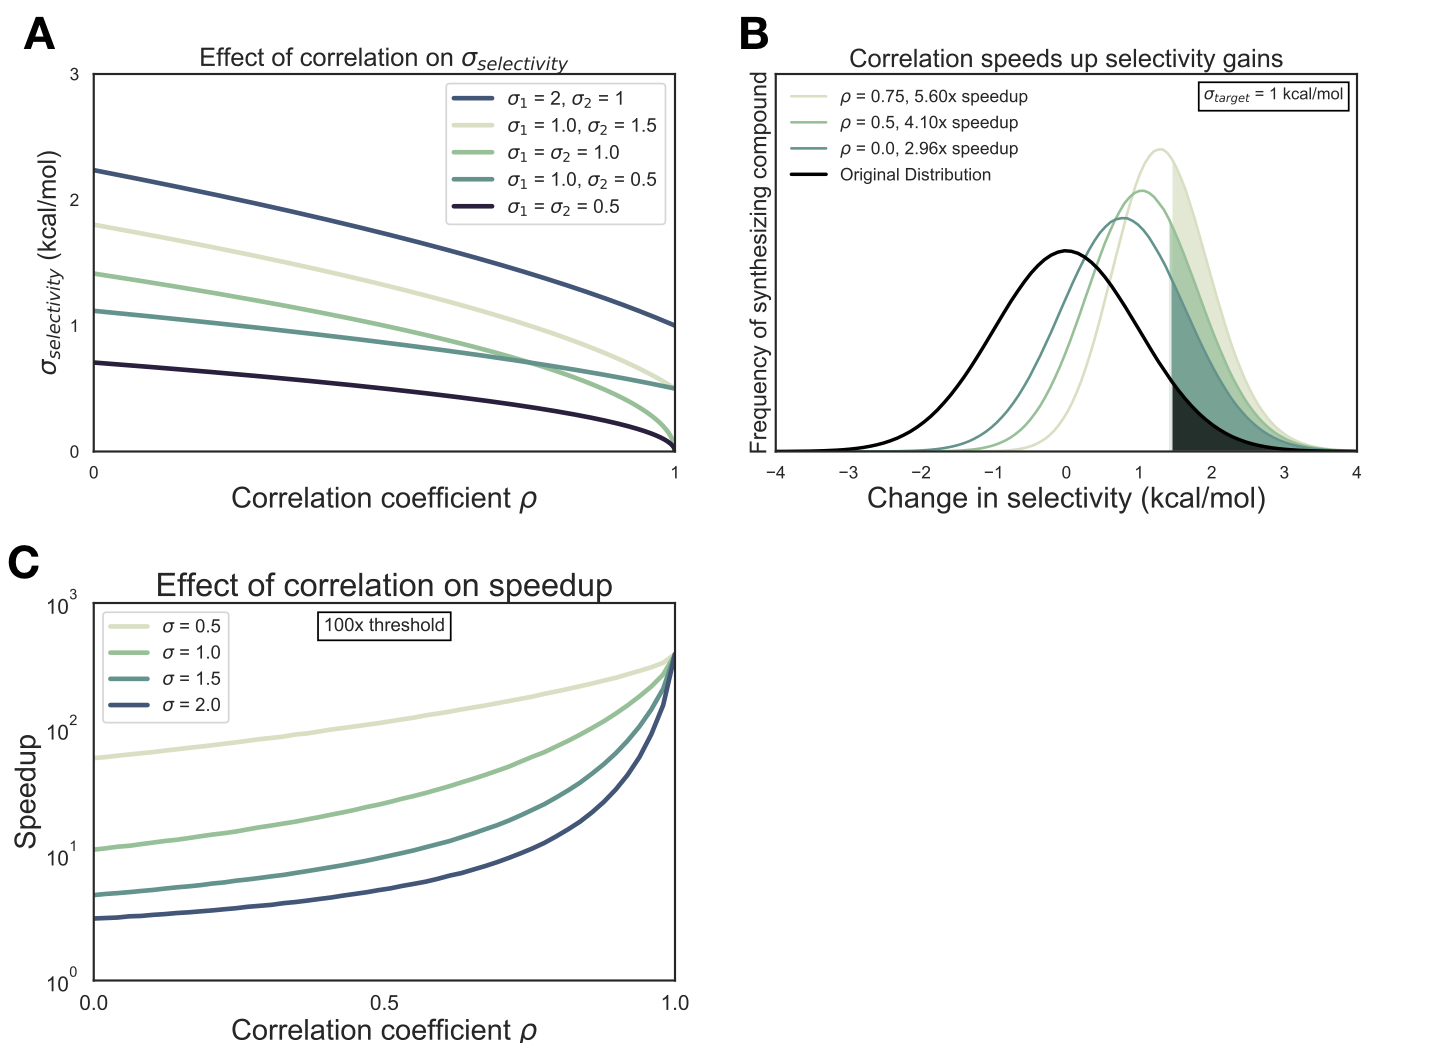
\includegraphics[width=0.9\textwidth]{figures/figure1.png}
  \caption[Free energy calculations speed up selectivity optimization]{{\bf Free energy calculations speed up selectivity optimization} ({\bf A})  The effect of correlation on expected errors for predicting selectivity ($\sigma_{selectivity}$) in kcal/mol. Each curve represents a different combination of target errors ($\sigma_1$ and $\sigma_2$). ({\bf B}) The change in selectivity for molecules proposed by medicinal chemists optimizing a lead candidate can be modeled by a normal distribution centered on 0 with a standard deviation of 1 kcal/mol (black curve). Each green curve corresponds to the distribution of compounds made after screening for a 1 log unit (1.4 kcal/mol) improvement in selectivity with a free energy methodology with a 1 kcal/mol per target error and a particular correlation. The shade region of each curve corresponds to the compounds with a real 1 log unit  improvement in selectivity. The speed up is calculated as the ratio of the percentage of compounds made with a real 1 log unit improvement to the percentage of compounds that would be expected in the original distribution.  ({\bf C}) The speedup (y-axis, log scale) expected for 100x (2 log units, 2.8 kcal/mol) selectivity optimization as a function of correlation coefficient $\rho$. Each curve corresponds to a different $\sigma_{target}$ value.
  }
 \label{fig:figure-1}
\end{figure}
\end{landscape}

\subsection{The CDK2 and CDK9 experimental dataset demonstrates the difficulty in achieving selectivity for closely related kinases}

To begin quantifying the correlation of errors in free energy predictions for selectivity, we set out to gather datasets that met a number of criteria. We looked for datasets that contained binding affinity data for a number of kinase targets and ligands, as well as having crystal structures for each target with the same co-crystallized ligand. For the CDK2/CDK9 datatset~\citep{Shao2013-oe}, ligand 12c was cocrystallized with CDK2/cylin A (Figure~\ref{fig:figure-2}A, left) and CDK9/cyclin T (Figure~\ref{fig:figure-2}B, left), work that was published in a companion paper~\citep{Hole2013-sr}. In both CDK2 and CDK9, ligand 12c forms relatively few hydrogen bond interactions with the kinase. Each kinase forms a set of hydrogen bonds between the ligand scaffold and a hinge residue (C106 in CDK9 and L83 in CDK2) that is conserved across all of the ligands in this series. CDK9, which has slightly lower affinity for ligand 12c (Figure~\ref{fig:figure-2}C, right), forms a lone interaction between the sulfonamide of ligand 12c and residue E107. On the other hand, CDK2 forms interactions between the sulfonamide of ligand 12c and residues K89 and H84. The congeneric series of ligands contains a number of challenging perturbations, particularly at substituent point R3 (Figure~\ref{fig:figure-2}C, left). Ligand 12i also presented a challenging perturbation, moving the 1-(piperazine-1-yl)ethanone from the \emph{meta} to \emph{para} location. 

This congeneric series of ligands also highlights two of the challenges of working from publicly available data. First, the dynamic range of selectivity is incredibly narrow, with a mean $\Delta \Delta G_{selectivity}$ (CDK9 - CDK2) of only -0.65 kcal/mol, and a standard deviation of 0.88 kcal/mol. Additionally, experimental uncertainties are not reported for the experimental measurements. Thus, for this and subsequent sets of ligands, the experimental uncertainty is assumed to be 0.3 kcal/mol based on previous work done to summarize uncertainty in experimental data~\citep{BROWN2009420,Hauser:2018vz}. 
\begin{landscape}
\begin{figure}[p]
\centering
	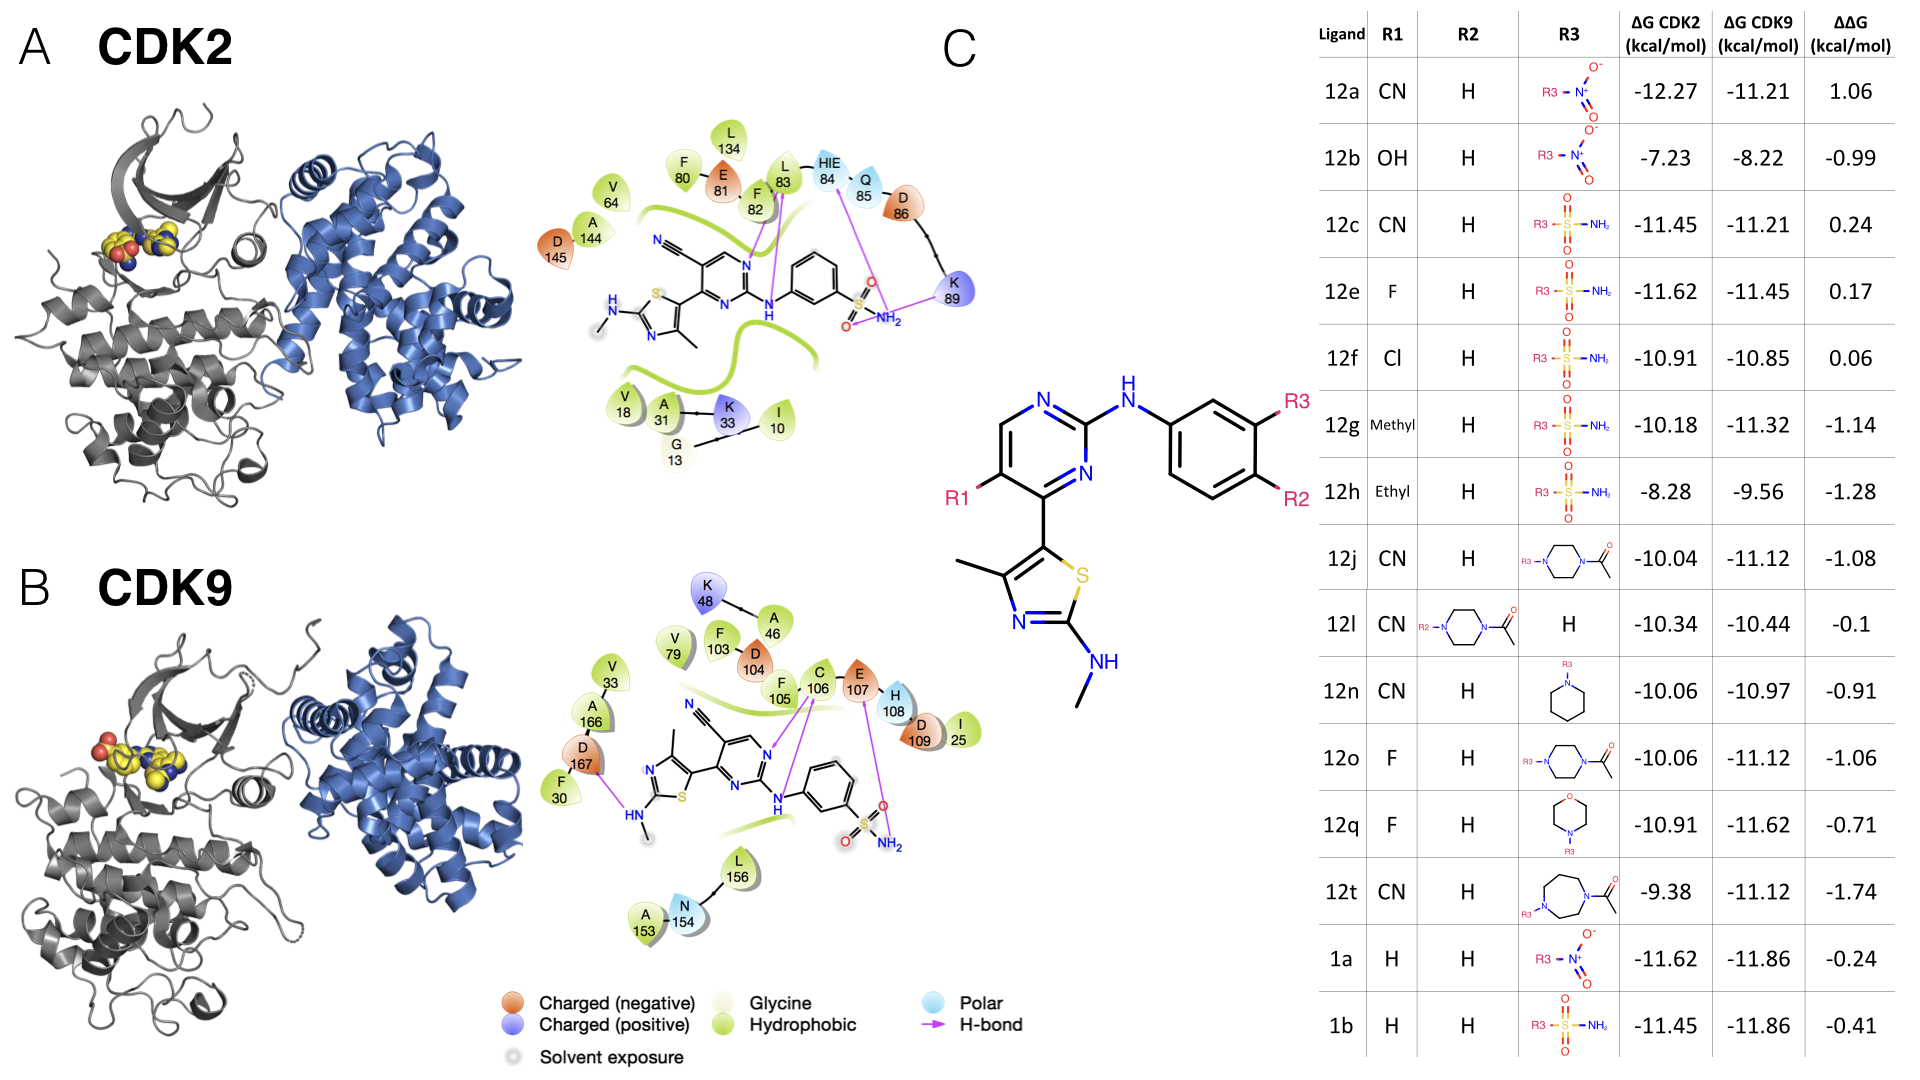
\includegraphics[width=1.0\linewidth]{figures/figure2.png}
	\caption[A CDK2/CDK9 selectivity dataset from Shao et \emph{al}., 2013]{{\bf A CDK2/CDK9 selectivity dataset from Shao \emph{et al.,} 2013}
({\bf A})  \emph{(left)} Crystal Structure (4BCK)\citep{Hole2013-sr} of CDK2 (gray ribbon)  bound to ligand 12c (yellow spheres). Cyclin A is shown in blue ribbon \emph{(right)} 2D ligand interaction map of ligand 12c in the CDK2 binding site. 
({\bf B}) \emph{(left)} Crystal structure of CDK9 (4BCI)\citep{Hole2013-sr} (gray ribbon) bound to ligand 12c (yellow spheres). Cyclin T is shown in blue ribbon. \emph{(right)} 2D ligand interaction map of ligand 12c in the CDK9 binding site.
({\bf C}) \emph{(left)} 2D structure of the common scaffold for all ligands in congeneric ligand series 12 from the publication \emph{(right)} A table summarizing all R group substitutions as well as the published experimental binding affinities and selectivities\citep{Shao2013-oe}. 
	}
	\label{fig:figure-2}
\end{figure}
\end{landscape}

\subsection{The CDK2 and ERK2 dataset achieves higher levels of selectivity for more distantly related kinases}
\todo{I probably need to either remove the reference to how closely related the kinases are, or come up with a way to quantify that - SKA}
The CDK2/ERK2 datatset from Blake \emph{et al.,} 2016 also met the criteria described above. Crystal structures for both CDK2 (Figure~\ref{fig:figure-3}A, top) and ERK2 (Figure~\ref{fig:figure-3}B, top) were available with ligand 22 co-crystallized. Of note, CDK2 was not crystallized with cyclin A, despite cyclin A being include in the affinity assay reported in the paper~\citep{Blake2016-su}. CDK2 adopts a DFG-in conformation with the $\alpha$C helix rotated out, away from the ATP binding site and breaking the conserved salt bridge between K33 and E51 (Supp. Figure~\ref{fig:sup-figure-1}A), indicative of an inactive kinase~\citep{Huse2002-ml,Hari:2013dp}. By comparison, the CDK2 structure from the CDK2/CDK9 dataset adopts a DFG-in conformation with the $\alpha$C helix rotated in, forming the ionic bond between K33 and E51 indicative of an active kinase, due to allosteric activation by cyclin A. While missing cyclins have caused problems for free energy calculations in prior work~\todo{is there a good citation for this?}, it is possible that the fully active conformation contributes equally to binding affinity for all of the ligands in the series, and the high accuracy of the potency predictions (Figure~\ref{fig:figure-4}, top left) is the result of fortutious cancellation of errors. The binding mode for this series is similar between both kinases. There is a set of conserved hydrogens bonds between the scaffold of the ligand and the backbone of one of the hinge residues (L83 for CDK2 and M108 for ERK2). The conserved lysine (K33 for CDK2 and K54 for ERK2), normally involved in the formation of a ionic bond with the $\alpha$C helix, forms a hydrogen bond with the scaffold (Figure~\ref{fig:figure-4}A and~\ref{fig:figure-4}B, bottom) in both CDK2 and ERK2. However, in the ERK2 structure, the hydroxyl engages a crystallographic water as well as N154 in a hydrogen bond network that is not present in the CDK2 structure. 
The congenric ligand series features a single subsituent point, with the R groups exposed to the solvent. This helps explain the extremely narrow distribution of selectivities, with a mean selectivity of -1.74 kcal/mol (ERK2 - CDK2) and standard deviation of 0.56 kcal/mol. This suggests that the selectivity is largely driven by the scaffold and unaffected by the R group substitutions.

\begin{landscape}
\begin{figure}[p]
\centering
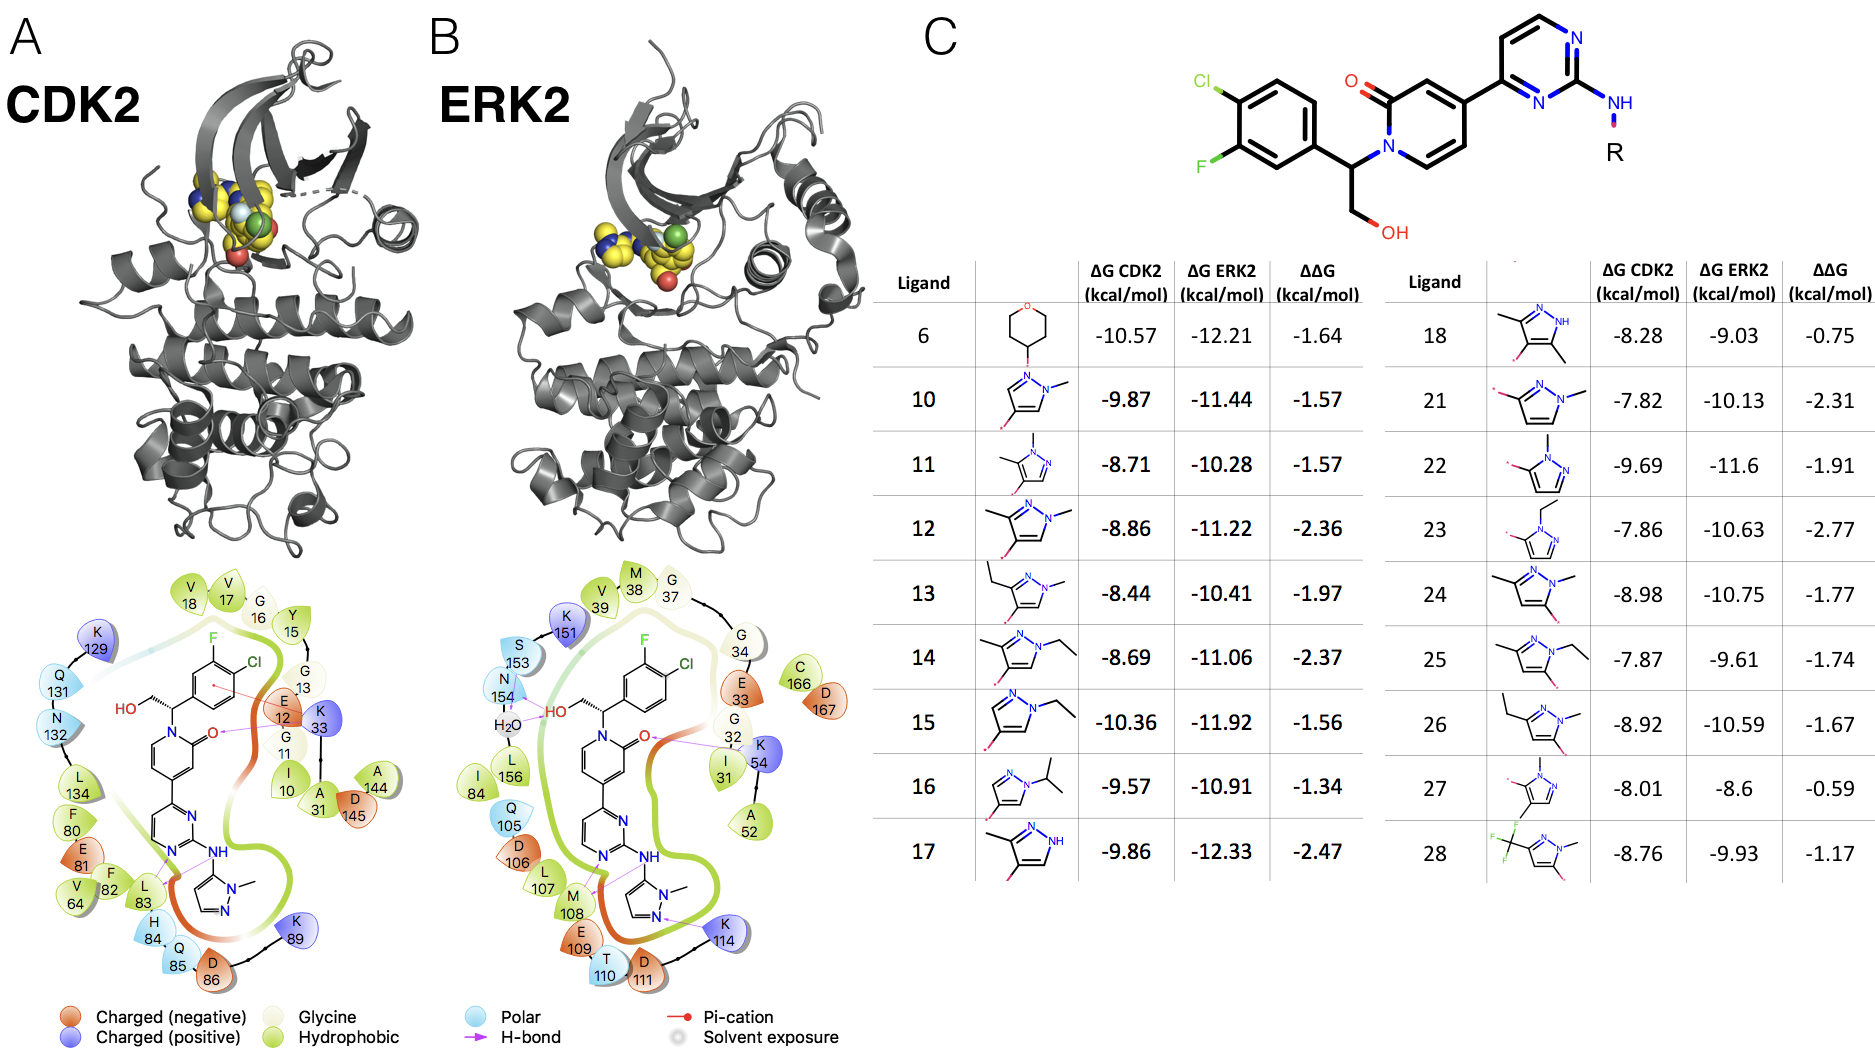
\includegraphics[width=1.0\linewidth]{figures/figure3.png}
\caption[CDK2 and ERK2 selectivity dataset from Blake et \emph{al}., 2016]{
{\bf CDK2 and ERK2 selectivity dataset from Blake et \emph{al}., 2016} \\
({\bf A})  \emph{(top)} Crystal structure of CDK2 (5K4J) shown in gray cartoon and ligand 22 shown in yellow spheres. \emph{(bot)} 2D interaction map of ligand 22 in the binding pocket of CDK2
({\bf B}) \emph{(top)} Crystal structure of ERK2 (5K4I) shown in gray cartoon with ligand 22 shown in yellow spheres. \emph{(bot)} 2D interaction map of ligand 22 in the binding pocket of ERK2.
({\bf C}) \emph{(top)} Common scaffold for all of the ligands in the Blake dataset, with R denoting attachment side for substitutions. \emph{(bot)} Table showing R group substitutions and experimentally measured binding affinities and selectivities. Ligand numbers correspond to those used in publication. 
}
\label{fig:figure-3}
\end{figure}
\end{landscape}

\subsection{FEP+ calculations show accurate potency predictions for ERK2/CDK2 and larger errors for CDK2/CDK9}
The FEP+ predictions of single target potencies ($\Delta G$) showed good accuracy for the CDK2 and ERK2 dataset (Figure~\ref{fig:figure-4}, top), with an RMSE of $0.37^{0.57}_{0.16}$ and $0.53^{0.81}_{0.22}$ kcal/mol, respectively. All of the CDK2 and ERK2 potencies were predicted within 1 log unit of the experimental value. Despite the high accuracy for the single target potency predictions, the selectivity ($\Delta \Delta G_{selectivity}$) predictions show an RMSE of $0.81^{1.26}_{0.37}$ kcal/mol, with all of the predictions falling within 1 log unit of the experimental values (Figure~\ref{fig:figure-4}, top right panel).\todo{this will change if we take of the ff uncertainty error bars}. Despite the high accuracy of the predictions, the narrow dynamic range and high uncertainty from experiment and calculation obscures any signal in the data. 
The CDK2 and CDK9 datasets show higher errors in the potency predictions, with an RMSE of $1.39^{2.05}_{0.58}$ and $1.71^{2.61}_{0.61}$ kcal/mol respectively. There are a number of outliers that fall outside of 1 log unit from the experimental value. While the higher per target errors make predicting potency more difficult, the selectivity predictions show a much lower RMSE of $0.74^{1.25}_{0.31}$ kcal/mol. This suggests that some correlation in the error is leading to fortuitous cancellation of systematic error, leading to more accurate than expected predictions of $\Delta \Delta G_{selectivity}$. 

\begin{landscape}
\begin{figure}
\centering
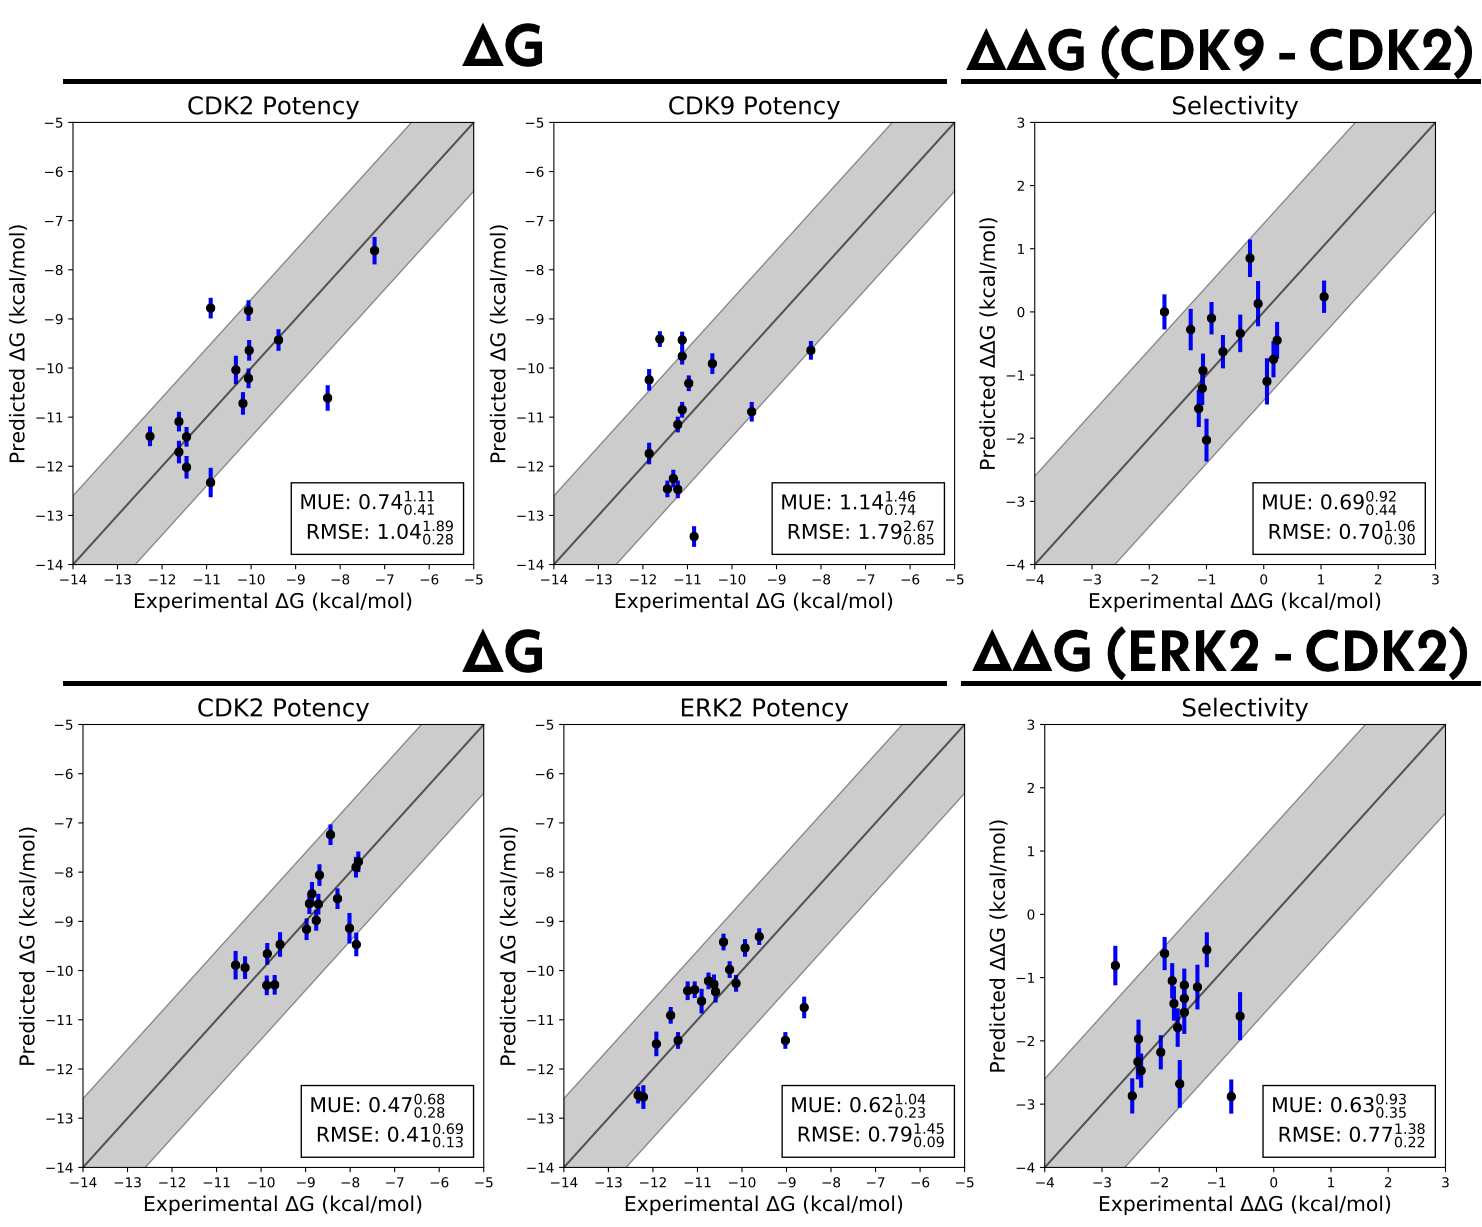
\includegraphics[width=0.6\linewidth]{figures/figure4.png}
\caption[Relative free energy calculations can accurately predict potency, but show larger errors for selectivity predictions.]{
{\bf Relative free energy calculations can accurately predict potency, but show larger errors for selectivity predictions.} \\
Single target potencies and selectivities for CDK2/ERK2 from the Blake datasets (\emph{top}), and CDK2/CDK9 (\emph{bottom}) from the Shao datasets. The experimental values are shown on the X-axis and calculated values on the Y-axis. Each data point corresponds to a ligand for a given target. All values are shown in units of kcal/mol. The horizontal error bars show the assumed experimental uncertainty of 0.3 kcal/mol\citep{BROWN2009420}. To better highlight outliers that are unlikely due simply to forcefield errors, we presume the forcefield error ($\sigma_\mathrm{FF} \approx$ 0.9 kcal mol$^{-1}$~\cite{Harder:J.Chem.TheoryComput.:2016}) also behaves as a random error. We show the total estimated statistical and forcefield error ($\sqrt{\sigma_\mathrm{FF}^2 + \sigma_\mathrm{calc}^2}$) as vertical blue error bars. The black vertical error bars correspond to the statistical error ($\sigma_{calc}$). The black line indicates agreement between calculation and experiment, while the gray shaded region represent 1.36 kcal/mol (or 1 log unit) error. The MUE and RMSE are shown on each plot with bootstrapped 95$\%$ confidence intervals.
}
\label{fig:figure-4}
\end{figure}
\end{landscape}

\subsection{Free energy calculation errors are correlated, accelerating selectivity optimization}
To quantify the correlation coefficient ($
\rho$) of the errors in our calculations, we built a Bayesian graphical model, as described in the methods section. Briefly, we modeled the absolute free energy ($G$) of each ligand in each phase (complex and solvent) as in equation~\ref{eq4}. The model was chained to the FEP+ calculations by providing the $\Delta G^{calc}_{phase,ij,target}$ as observed data, as in equation~\ref{eq6}. As in equation, the experimental data was modeled as a normal distribution centered around the true free energy of binding ($\Delta G^{true}_{i,target}$) corrupted by experimental error, which is assumed to be 0.3 kcal/mol from previous work done to quantify the uncertainty in publicly available data~\citep{BROWN2009420}. The reported IC50 values from each dataset were treated as data observations (Equation~\ref{eq12}) and the $\Delta G^{true}_{i,target}$ was assigned a weak normal prior (Equation~\ref{eq13}). The correlation coefficient was calculated for each sample according to equation~\ref{eq9}. 
The correlation coefficient $\rho$ for the CDK2/ERK2 calculations was quantified to be $0.5^{0.33}_{-0.23}$, indicating that the errors are largely uncorrelated between ERK2 and CDK2 (Figure~\ref{fig:figure-5}A, right). The joint marginal distribution of the error ($\epsilon$) for each target is symmetric, which is expected for cases in which $\rho$ is 0 (Supp. Figure~\ref{fig:sup-figure-2}). Despite the weak correlation in errors, the high per target accuracy of these calculations should have a 2-3x speed up for 1 log unit selectivity optimization, and a 20-30x speed up for 2 log unit selectivity optimization (Figure~\ref{fig:figure-5}A, right). 
The CDK2/CDK9 calculations show strong evidence of correlation, with a correlation coefficient of $0.70^{0.82}_{0.57}$ (Figure~\ref{fig:figure-5}B, right). The joint marginal distribution of errors is strongly diagonal, which is expected based on the value for $\rho$ (Figure~\ref{fig:figure-5}B, left). The high correlation in errors leads to a speed up of 4-5 for 1 log unit selectivity optimization and 30-40x for 2 log unit selectivity optimization (Figure~\ref{fig:figure-5}B, right), despite the much higher per target errors.
Quantifying $\rho$ for these calculations enables estimation of $\sigma_{selectivity}$, which is useful for estimating expected error for prospective studies, where the experimental values for $\Delta \Delta G_{selectivity}$ are not yet known. Based on the distribution quantified for $\rho$, the expected $\sigma_{selectivity}$ for the CDK2/CDK9 calculations is between 0.76 and 1.16 kcal/mol (Supp. Figure~\ref{fig:sup-figure-3}), which is in good agreement with the bootstrapped RMSE (Figure~\ref{fig:figure-4}, bottom). For the CDK2/ERK2 calculations, $\sigma_{selectivity}$ is expected to fall between 0.82 kcal/mol and 1.10 kcal/mol (Supp. Figure~\ref{fig:sup-figure-3}), which is also in good agreement with the bootstrapped RMSE (Figure~\ref{fig:figure-4}, top). 

\begin{landscape}
\begin{figure}
\centering
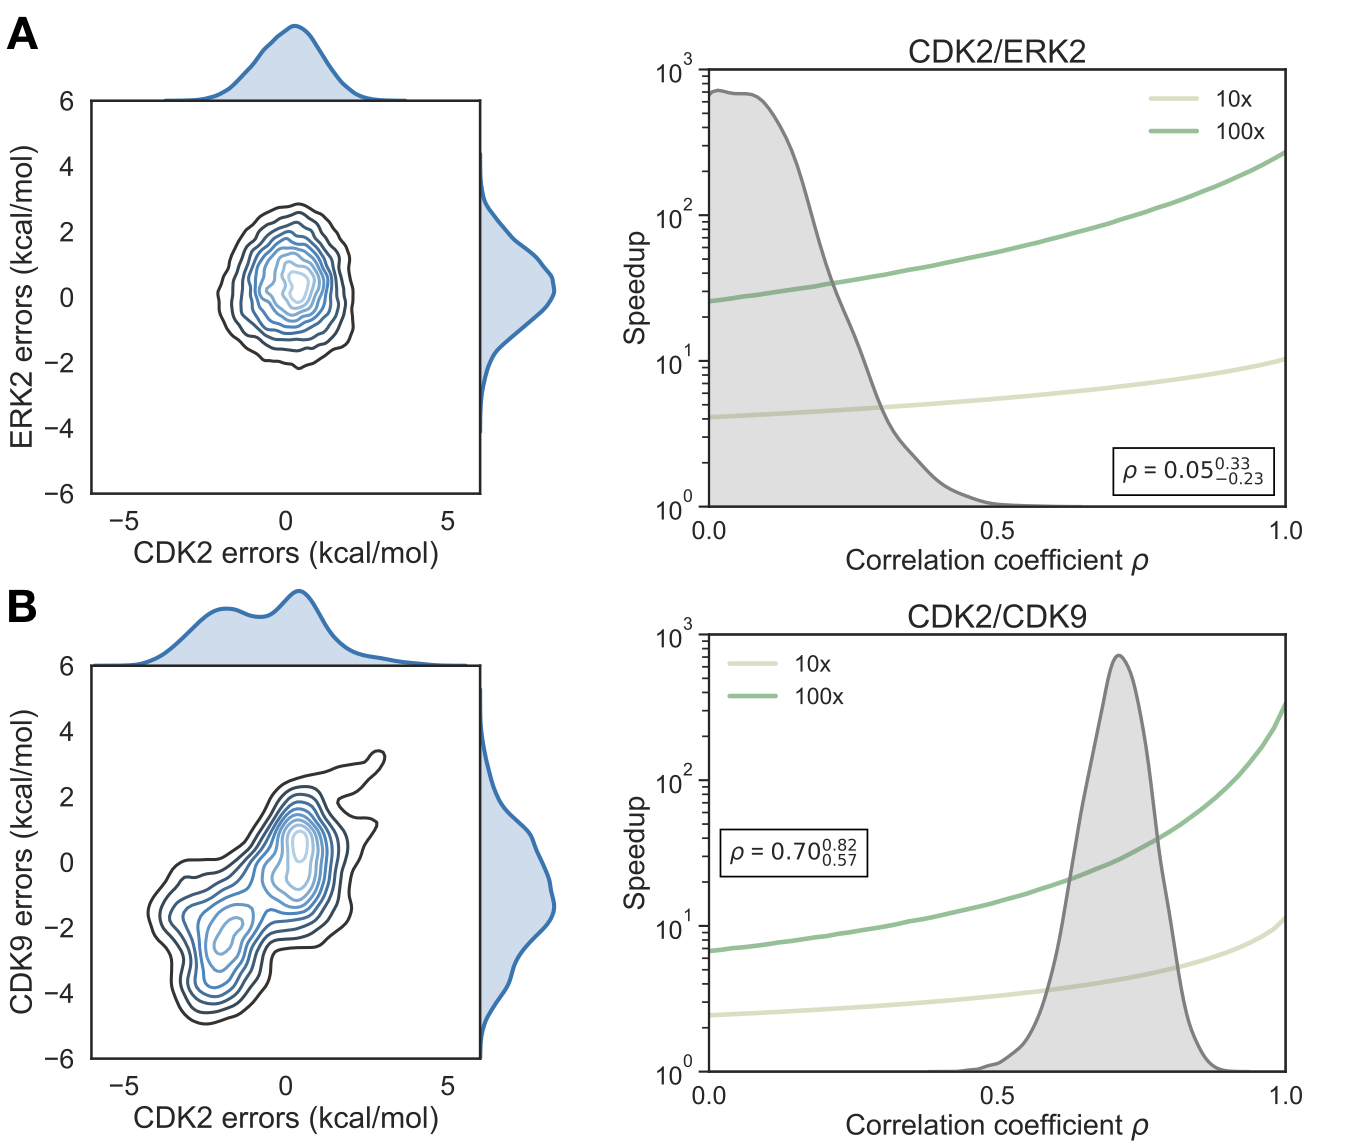
\includegraphics[width=0.7\linewidth]{figures/figure5.png}
\caption[Correlation in selectivity prediction errors can be used to accelerate selectivity optimization]{
{\bf Correlation in selectivity prediction errors can be used to accelerate selectivity optimization} \\
({\bf A}) (\emph{left}) The joint posterior distribution of the prediction errors for CDK2 (X-axis) and ERK2 (Y-axis) from the Bayesian graphical model. (\emph{right}) Speedup in selectivity optimization (Y-axis) as a function of correlation coefficient (X-axis). The posterior marginal distribution of the correlation coefficient ($\rho$) is shown in gray, while the expected speed up is shown for 100x (green curve) and 10x (yellow curve) selectivity optimization. The inserted box shows the mean and 95\% confidence interval for the correlation coefficient. 
({\bf B}) (\emph{left}) The same as above, with CDK2 (X-axis) and CDK9 (Y-axis). (\emph{right}) As above, for the CDK2/CDK9 calculations.
}
\label{fig:figure-5}
\end{figure}
\end{landscape}

\section{Discussion and Conclusions}
We have demonstrated, using a simple numerical model, the impact that free energy calculations with even weakly correlated errors can have on speeding up the optimization of selectivity in small molecule kinase inhibitors. While the expected speed up is dependent on the per target error of the method ($\sigma_{target}$), the speedup is also highly dependent on the correlation of errors made for both targets. Unsurprisingly, free energy methods have greater impact as the threshold for selectivity optimization goes from 10x to 100x. While 100x selectivity optimization is difficult to achieve, the expected benefit from free energy calculations is also quite high, with 1 and 2 order of magnitude speedups possible. 
To quantify the correlation of errors in two example systems, we gathered experimental data for two congeneric ligand series with experimental data for CDK2 and ERK2, as well as CDK2 and CDK9. These datasets, which had crystal structures for both targets with the same ligand co-crystallized, are exemplify the difficulty in predicting selectivity. The dynamic range of selectivity for both systems is incredibly narrow, with most of the perturbations not having a major impact on the overall selectivity achieved. Furhter, the data was reported with unrelaible experimental uncertainties, which makes quantifying the errors made by the free energy calculations difficult. This issue is common when considering selectivity, as many kinase-oriented high throughput screens are carried out at a single concentration and not highly quantitative. Work is being done to increase the availability of publicly available, high quality biophysical data for selectivity measurements, which will benefit future work on predicting selectivity using physical models and machine learning techniques. 
\todo[inline]{insert a discussion of outliers in the FEP+ calculations here?}
\todo[inline]{discuss quantification of rho (is there a way to know a priori what rho might be?)}
\todo[inline]{discussion of the expected speedup and sigma based on the quantification of rho}
\todo[inline]{extensions include: separating statistical error (unless this gets added into the results section}
\todo[inline]{Do we want to mention protein mutation FEP+ to enable cycle closure analysis for certain highly related targets?}

\begin{landscape}
\begin{figure}[p]
\centering
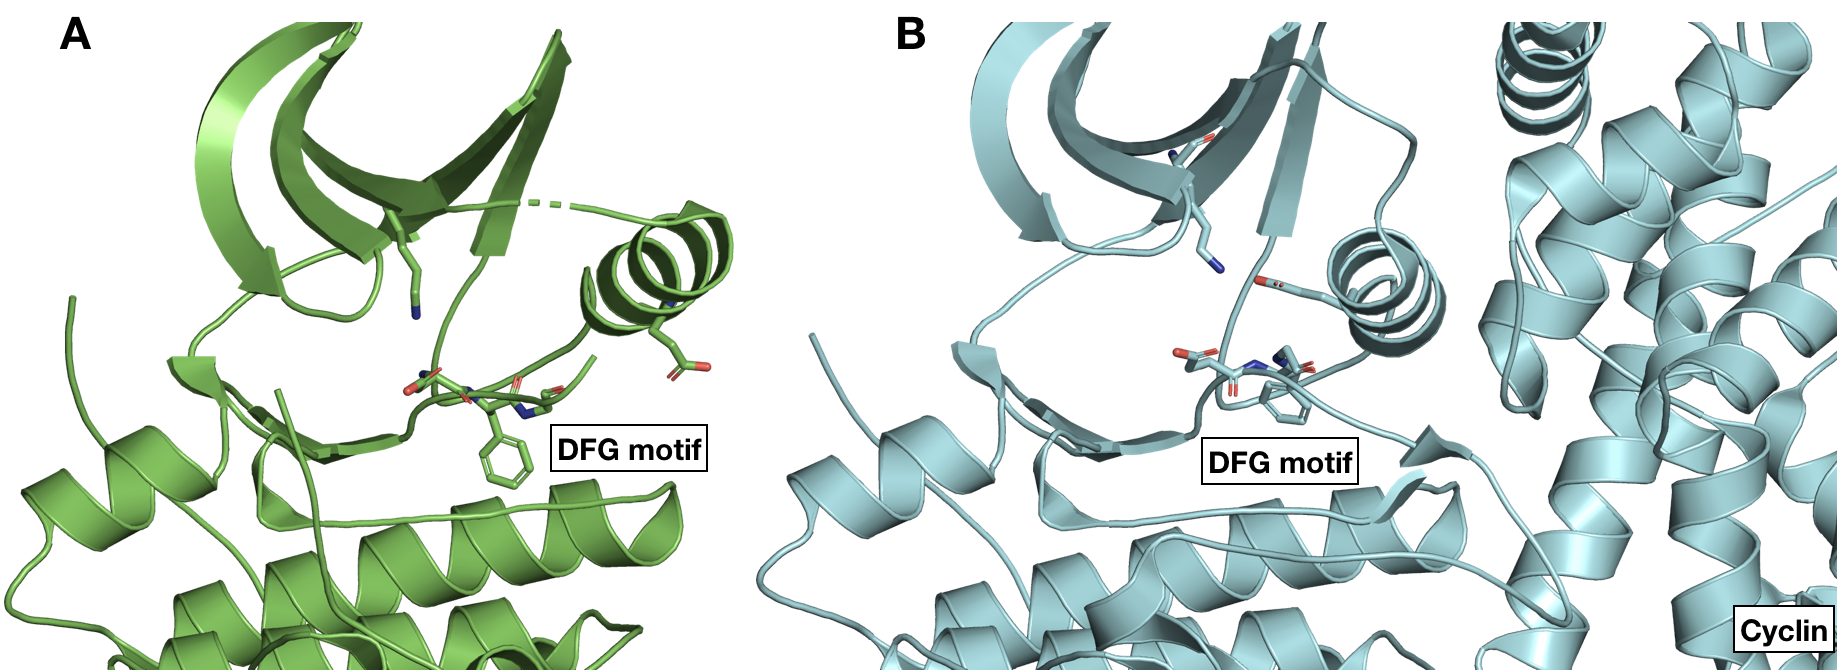
\includegraphics[width=1.0\linewidth]{figures/supp_figure1.png}
\caption[CDK2 adopts an inactive conformation in the crystal structure used for the CDK2/ERK2 calculations]{
{\bf CDK2 adopts an inactive conformation in the crystal structure used for the CDK2/ERK2 calculations} 
({\bf A}) CDK2 (5K4J) adopts an inactive conformation in the absence of its cyclin. The DFG motif is in a DFG-in conformation, with the $\alpha$C helix rotated outwards, breaking the salt bridge between K33 and E51 (Uniprot numbering) that is typically a marker of an active conformation. Notably, the Phe in the DFG motif does not completely form the hydrophobic spine due to the rotation of the $\alpha$C helix~\citep{Hu:2015kh}
({\bf B}) The CDK2 structure used for the CDK2/CDK9 calculations (4BCK) contains cyclin A and adopts a DFG-in/$\alpha$C helix-in conformation that forms the salt bridge between K33 and E51. This is typically indicative of a fully active kinase~\citep{Huse2002-ml,Hari:2013dp}. 
}
\label{fig:sup-figure-1}
\end{figure}
\end{landscape}

\begin{landscape}
\begin{figure}[p]
\centering
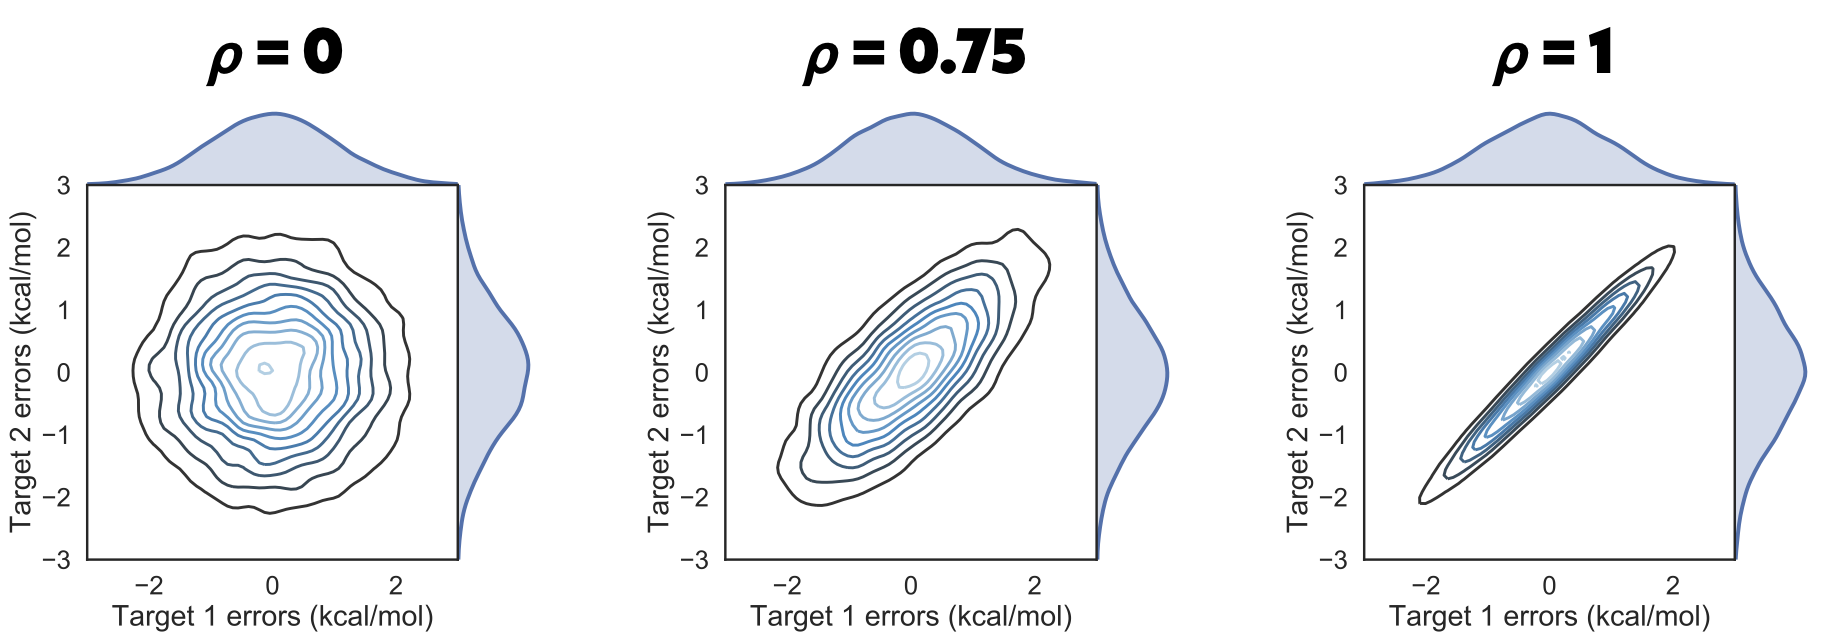
\includegraphics[width=1.0\linewidth]{figures/supp_2.png}
\caption[ Correlation coefficient $\rho$ controls the shape of the joint marginal distribution of errors]{
{\bf Correlation coefficient $\rho$ controls the shape of the joint marginal distribution of errors} 
As $\rho$ increases, the joint marginal distribution of errors become more diagonal. Each panel shows 10000 samples drawn from a multivariate normal distribution centered around 0 kcal/mol, where the per target error was set to 1 kcal/mol and $\rho$ to the value indicated in bold over the plot. 
}
\label{fig:sup-figure-2}
\end{figure}
\end{landscape}

\begin{landscape}
\begin{figure}[p]
\centering
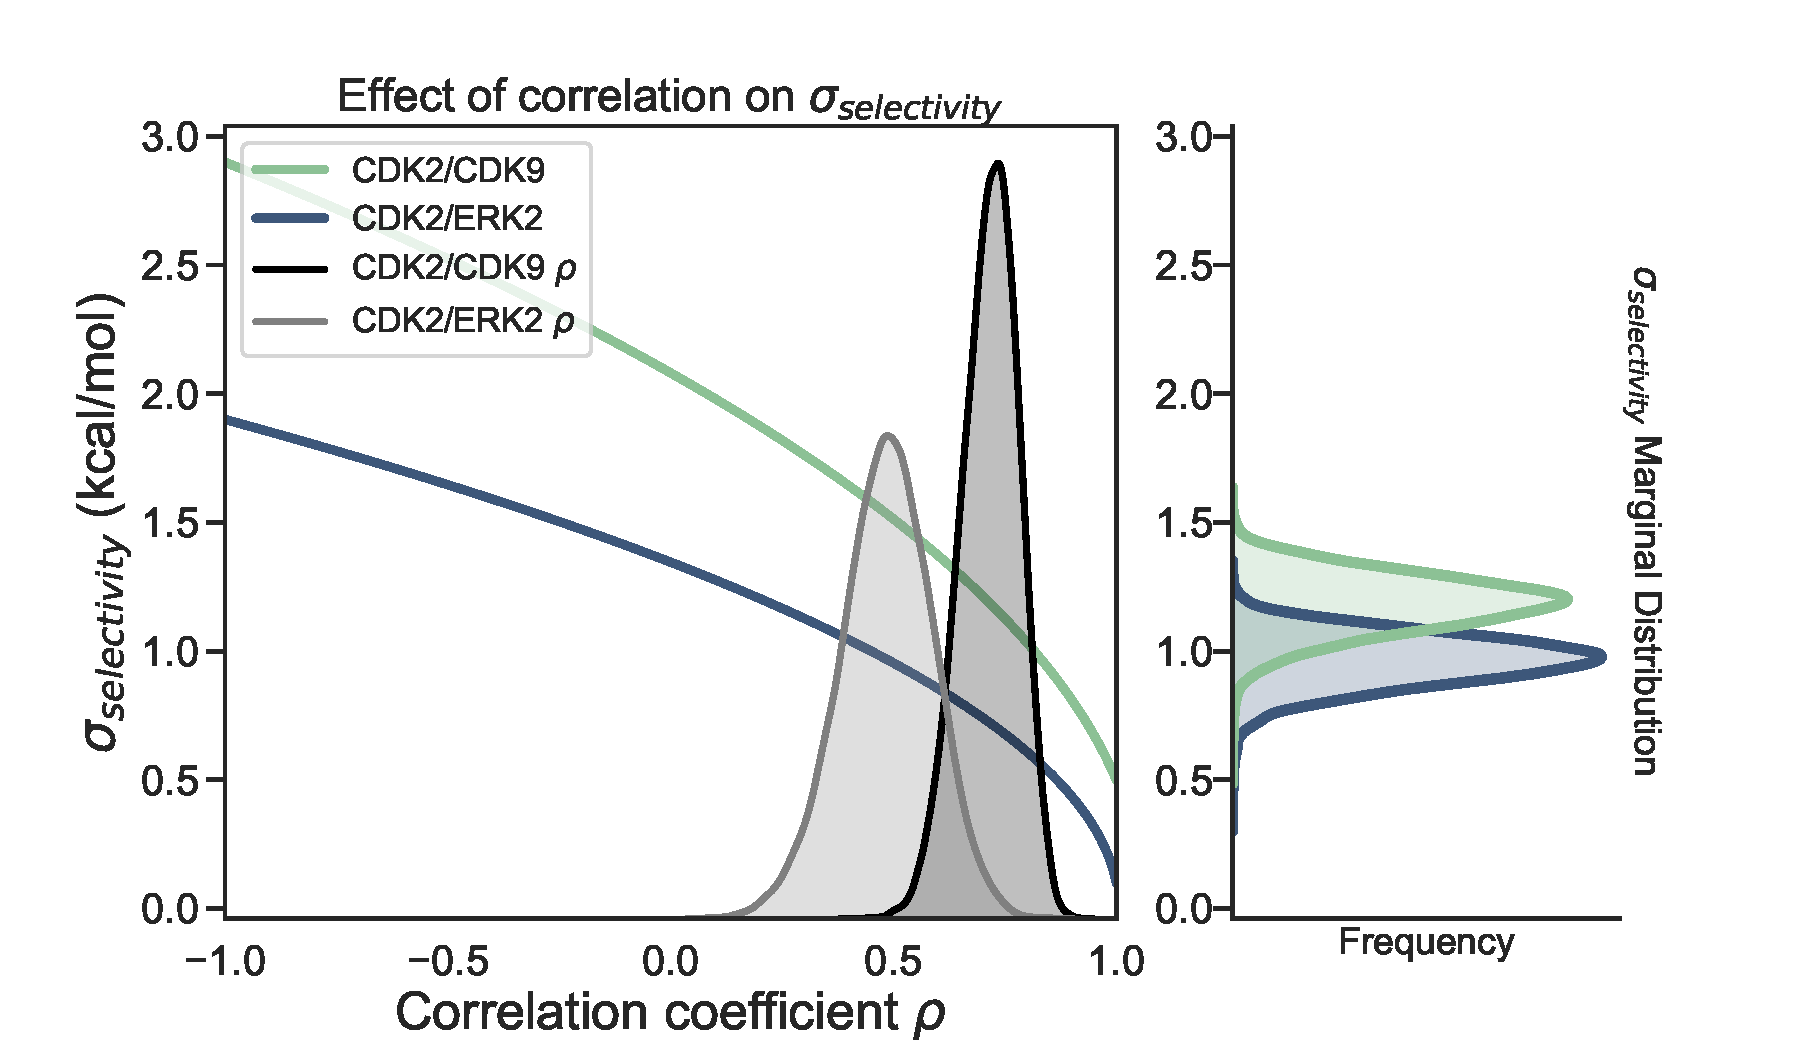
\includegraphics[width=0.8\linewidth]{figures/supp_figure3.pdf}
\caption[Correlation reduces the expected error for selectivity predictions]{
{\bf Correlation reduces the expected error for selectivity predictions}
As corelation coefficient $\rho$ increases, $\sigma_{selectivity}$ decreases. The intersection between CDK2/CDK9 $\sigma_{selectivity}$ (green curve) and $\rho$ (black distribution) indicates the range of expected $\sigma_{selectivity}$ values. The intersection for CDK2/ERK $\sigma_{selectivity}$ (blue curve) and $\rho$ (gray distribution) suggests the expected $\sigma_{selectivity}$ range for that set of calculations. 
}
\label{fig:sup-figure-3}
\end{figure}
\end{landscape}

\chapter{Understanding the functional impact of mTOR clinical kinase mutations using physical modeling}

\section{Introduction}
\subsection{mTOR forms the catalytic core of protein complexes that control a number of cellular processes}
mTOR (mammalian target of rapamycin) is a serine-threonine kinase that controls a number of cellular processes~\citep{Laplante:2012fm,Saxton:2017cv} by integrating signaling from the MAPK and PI3K pathways~\citep{Mendoza2011-bj}. mTOR forms the catalytic core of heteromeric protein complexes, mTORC1 and mTORC2, that differ in the regulatory proteins that decorate the kinase. mTORC1 is defined by RAPTOR~\citep{Kim:2002vh,Hara:2002tn} and PRAS40~\citep{Yang:2017gu}, while mTORC2 is characterized by RICTOR~\citep{Sarbassov:2004kv}. Each complex contains a number of shared regulatory proteins, such as mLST8~\cite{BarPeled:2012gq} and DEPTOR~\citep{Peterson:2009fc}. mTOR itself is an atypical kinase, and includes a number of insertions that deviate from the canonical kinase fold. The C-terminal fragment crystal structure (Figure~\ref{fig:mtor-figure1})shows that the kinase domain is hugged by a FAT domain~\citep{Yang:2013gaa}, forming a C-shaped clamp around the kinase domain. The FAT domain forms a number of regulatory salt bridges that have been implicated in controlling the activity of the kinase~\cite{Yang:2013gaa}. The FK506-rapamycin-binding (FRB) domain hangs over the opening cleft to the active site~\cite{Yang:2013gaa} (Figure~\ref{fig:mtor-figure1}). The FRB domain is exposed in mTORC1, while is it thought to be occluded and inaccesible to FKBP12 in mTORC2~\citep{Gaubitz:2015gr}. Complex activity is hypothesized to be regulated via restricted access to the active site by architectural elements as well as rapalog-mediated recruitment of FKBP to the FRB domain~\citep{Aylett:2016gs}. 

\begin{landscape}
	\begin{figure}[p]
		\centering
		\includegraphics[width=0.8\linewidth]{figures/mtor-fig1.pdf}
		\caption[mTOR is an atypical kinase with a number of regulatory domains]{
			{\bf mTOR is an atypical kinase with a number of regulatory domains}
			mTOR (PDBID: 4JSV) is shown as a cartoon diagram. The kinase domain (white) has a number of structural features highlighted, such as the activation loop (teal) as well as a network of regulatory $\alpha$ helices (red) in the active site. The FAT domain (black) clamps around the kinase domain and forms a number of salt bridge and hydrophobic contains with the kinase domain. The FRB domain (gold) hangs over the active site clef and is the site of rapalog binding and rapalog-mediate FBKBP recruitment. \bf{This figure reprinted with permission of James Hsieh}
		}
		\label{fig:mtor-figure1}
	\end{figure}
\end{landscape}

mTORC1 controls a number of biological processes by integrating multiple upstream signals (Figure~\ref{fig:mtor-figure2}). Tuberous sclerosis complex 1/2 (TCS1/2) integrates growth factor signaling from the PI3K/AKT pathway~\citep{Inoki:2002jv,Manning:2002tp} and DNA damage from AMPK~\citep{Jones:2005kg}. TSC1/2 acts as GTPase activating protein (GAP) for RHEB~\citep{Inoki:2003je}, which binds to and activates mTORC1 at the lysosomal surface. mTORC1 localization is controlled by the second major signal it integrates: amino acid availability. Upon stimulation by amino acids, the Ragulator~\citep{BarPeled:2012fr} recruits inactive mTORC1 from the cytosol to the lysosomal surface~\citep{Kim:2008kb,Sancak:2010bu,Efeyan:2012de}, enabling interaction with RHEB. Once active, mTORC1 controls cell growth and protein synthesis by phosphorylating and activating S6K at T389 and inactivating 4EBP1 via a phosphorylation at S65~\citep{Hay:2004ir,Laplante:2012fm}. mTORC1 also activates SREBP1/2, which regulates lipid biosynthesis~\citep{Lamming:2013dza}. mTORC1 activation inhibits autophagy through via ULK1. Recent work suggests that mTORC1 can also control the biophysical properties of the cytoplasm by regulating crowding~\citep{Delarue:2018ca}, impacting the rate of diffusion and expanding the already diverse array of essential processes that mTOR controls. 

\subsection{mTOR is the targeted by inhibitors with two distinct mechanisms of action}
Due to the central role mTOR plays in a wide array of biological processes, it has emerged as the target of extensive drug discovery programs. There are two distinct classes of inhibitors developed to target mTOR: ATP-competitive inhibitors and allosteric inhibitors~\citep{Ballou:2008ec,Lamming:2013kg}. Temsirolimus~\citep{Hudes:2007kp} and Evirolimus~\citep{Motzer:2008cn} are FDA-approved inhibitors~\citep{fda-approved-kinase-inhibitors} that are thought to inhibit mTOR through recruiting FKBP family members, such as FKBP12, to the FRB domain~\citep{Hausch:2013iu}. Evidence suggests FKBP12 recruitment may inhibit mTORC1 activity by inducing a conformational change that prevents S6K binding~\citep{Yip:2010bm}. Further incubation leads to destabilization and disassembly of the protein complex, which is consistent with the time-dependent nature of rapalog inhibition of mTORC1 mediated 4EBP1 phosphorylation~\citep{Yip:2010bm}. The rapalogs are potent inhibitors of mTORC1, while mTORC2 requires chronic rapalog treatment and is highly dependent on FKBP expression levels~\citep{Schreiber:2015fi}. A cryo-EM structure of TORC2 suggests that the FRB domain is inaccessible in TORC2, explaining the relative insensitivity of mTORC2 to rapalog inhibition~\citep{Gaubitz:2015gr}. Rapalogs have also been shown to only partially inhibit mTORC1, often failing to reduce 4EBP phosphorylation levels~\citep{Saxton:2017cv}, despite efficacy at preventing S6K phosphorylation. 
There are an array of ATP-competitive inhibitors developed to target mTOR and other members of the PI3K family of kinases, such as MLN0128~\citep{Slotkin:2015je,Hassan:2014kl}, INK-228 (TAK-128)~\citep{GarciaGarcia:2012jc}, AZD8055~\citep{Chresta:2010ir}, PKI-587~\citep{Mallon:2011gn}, and BEZ-235~\citep{Mukherjee:2012ki}. ATP-competitive inhibitors exhibit a wide range of selectivity, with many inhibiting mTORC1, mTORC2, and multiple isoforms of PI3K. ATP competitive inhibitors target the catalytic activity of mTOR and more fully inhibit mTORC1 and mTORC2 phosphorylation of downstream targets~\citep{Saxton:2017cv}. While many of these inhibitors have struggled clinically due to modest clinical benefits and high toxicity leading to low tolerability~\citep{Pongas:2016jm}, there is considerable excitement about developing mTOR inhibitors to treat a number of diseases. ATP-competitive inhibitor BEZ-235 has shown promising results in preclinical models of lapatinib-resistant PI3K hyperactivated breast cancer~\citep{Eichhorn:2008ff}.  Dual targeted catalytic inhibitors that target both PI3K and mTOR have shown success by abrogating reactivation of Akt, which is caused by the alleviation of negative feedback due to long term treatment with mTOR inhibitors~\citep{RodrikOutmezguine:2011fb}. For example, a dual-inhibitor of mTORC and PI3K$\alpha$, PI-103, showed promising activity against glioma xenografts~\citep{Fan:2006kw}. 

mTOR inhibitors show the most promise in treating diseases with mTOR pathway alterations pathway~\citep{Wagle:2014ej}. Despite initial success, resistance mutations in the FRB or kinase domain have been observed~\citep{Wagle:2014be}. Work has also been done to combine the two mechanisms of action in Rapalink-1, which tethers rapamycin and MLN0128~\citep{RodrikOutmezguine:2016km} with a flexible linker and overcome such acquired resistance. Rapalink also shows improvements over ATP-competitive inhibitors or rapalogs outside of the context of resistance.  In glioblastoma models, ATP-competitive inhibitor MLN0128 and allosteric inhibitor rapamycin showed poor \emph{in vivo} efficacy. In contrast, RapaLink-1, by overcoming poor residence time and potency, was able to durably inhibit mTORC1 and cross the blood-brain barrier~\citep{Fan:2017fk}. 

\begin{landscape}
	\begin{figure}[p]
		\centering
		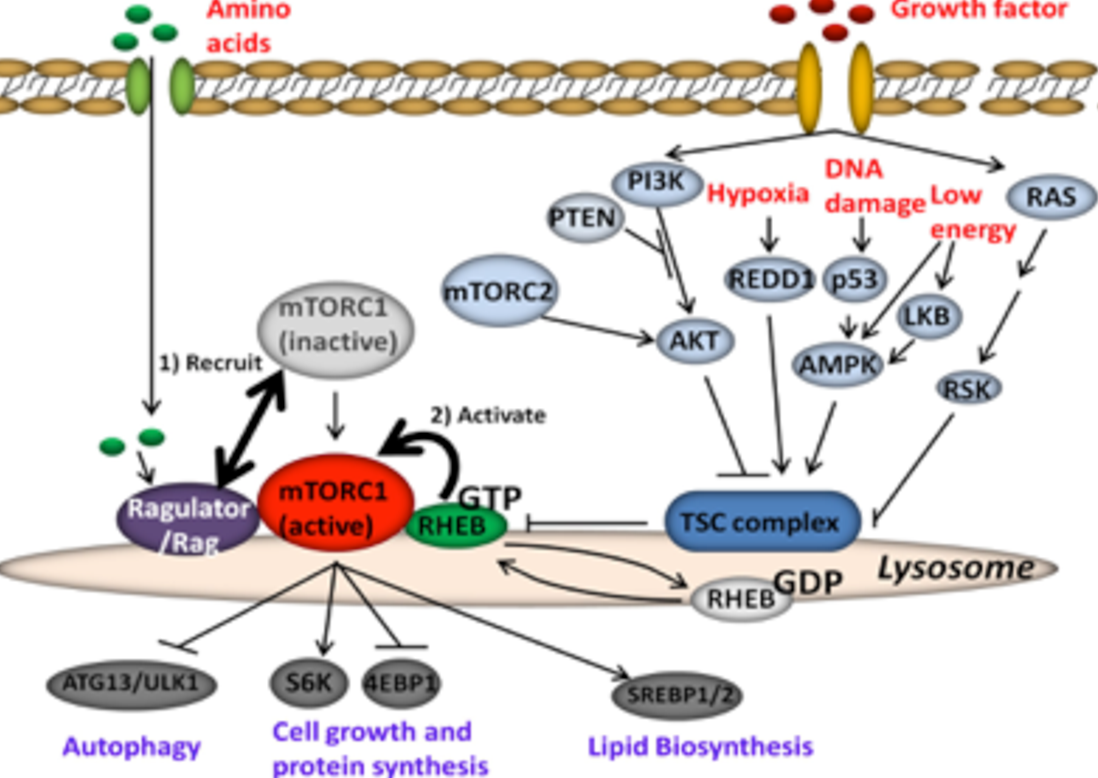
\includegraphics[width=0.8\linewidth]{figures/mtor-fig2.pdf}
		\caption[mTORC1 integrates signaling from a number of inputs]{
			{\bf mTORC1 integrates signaling from a number of inputs}
			The signaling pathway of mTOR involves integrating signaling from the growth factors, amino acids, hypoxia, and DNA damage. Integrating such signals controls the localization and activity of mTORC1, which controls autophagy, cell growth, and macromolecule synthesis through phosphorylation of downstream targets. \bf{This figure courtesy of James Hsieh} 
		}
		\label{fig:mtor-figure2}
	\end{figure}
\end{landscape}

\subsection{mTOR signaling is dysregulated in cancer by hyperactivating missense mutations}
mTOR pathway alterations have been observed in a wide array of cancer types~\citep{Guertin:2007dw} and extensively characterized. Less well studied are missense mutations in mTOR itself. An exceptional responder in a phase 1 clinical trial of pazopanib and everolimus with metastatic urothelial carcinoma lead to the identification of two missense mutations in mTOR~\citep{Wagle:2014ej}, E2014K and E2419K. Subsequent work identified 33 MTOR mutations gathered from publicaly available tumor sequencing data, and found that a number of them activated the mTOR pathway and conferred sensitivity to mTOR inhibitors when engineered into various cancer cell lines \emph{in vitro}~\citep{Grabiner:2014be}. While these missense mutations are pulled from an array of different cancer types, mTOR missense mutations have been observed in about 15\% of clear cell renal cell carcinoma~\citep{CancerGenomeAtlasResearchNetwork:2013ib}. Characterization of these mutations revealed that not only do many of these mutations hyperactivate mTOR (Figure ~\ref{fig:mtor-figure3}), but they can be grouped into complementation groups by determining which double mutations cause hyperactivation at levels higher than the constituent single mutants alone~\citep{Xu:2016fw}. This suggests that these mutations can activate mTOR through different, seemingly complementary mechanisms. 

\begin{landscape}
	\begin{figure}[p]
		\centering
		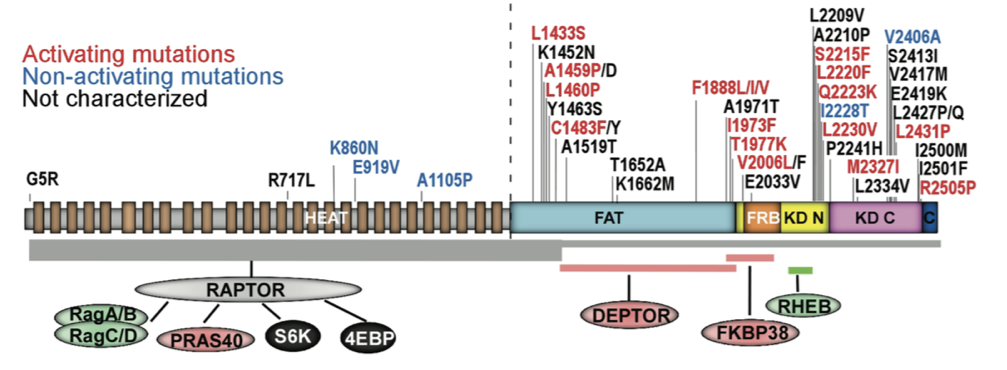
\includegraphics[width=1.0\linewidth]{figures/mtor-fig3.png}
		\caption[Hyperactivating mTOR missense mutations have been observed in cancer]{
			{\bf Hyperactivating mTOR missense mutations have been observed in cancer}
			Diagram shows the domain structure of mTOR, its regulatory interaction partners (negative regulators in pink, positive regu- lators in green, and a dual-role regulator in gray), and the substrates of mTORC1 complex. The positions within mTOR that are involved in the interaction with the regulatory partners are highlighted below the domain structure. The thickness of the horizontal bar of RAPTOR-mTOR interaction indicates the relative binding affinity. mTOR missense mutations derived from ccRCC are mapped and color coded
			to summarize their respective effects on mTORC1 signaling (activating mutations in red). KD N, kinase domain N lobe; KD C, kinase domain C lobe. \bf{This figure reprinted with permission of James Hsieh and the Journal of Clinical investigation~\citep{Xu:2016fw}.}
		}
		\label{fig:mtor-figure3}
	\end{figure}
\end{landscape}

\subsection{Using physical modeling to understand the functional impact of mTOR mutations}
To begin to understand the impact of these missense mutations at an atomistic level, we performed massively parallel molecular dynamics~\citep{Salsbury:2010ij} using the computing resource Folding@Home~\citep{Shirts:2000du}. Molecular Dynamics simulations have been used previously to understand the mechanism of oncogenic and resistance mutations on the structure and activation of EGFR~\citep{Shan:2012bs,Sutto:2013gy}. They have also been applied to understanding missense mutations in p53~\citep{Demir:2011bc}, CLIC2~\citep{Witham:2011co}, opsin~\citep{Tsukamoto:2013gr}, and a host of oncogenes and tumor suppressors\citep{Stehr:2011ga}. Using the previously solved crystal structure~\citep{Yang:2013gaa}, we built models for 45 single, and 190 double mutations, far more than could be crystallized individually~\citep{Xu:2016fw}. We analyzed the simulations for changes in contact formation, as well as changes in order parameters for activation mined from other kinase studies and previous work on mTOR biochemistry. We also piloted alchemical free energy calculations~\citep{Chodera:Curr.Opin.Struct.Biol.:2011} on a number clinically observed mutants, to compute physical, testable properties such as change in affinity for ATP-competitive inhibitors and ATP itself. In doing so, we identify promising candidates for resistance mutations to an ATP competitive inhibitor, and lay the ground work for future studies on the application of these methods to studying the functional impact of mutations on inhibitor binding. Taken together, this work forms the beginning of a comprehensive analysis of the impact of these mutations on structure and small molecule binding, which has implications for the treatment of patients with these mutations. 


\section{Methods}
\subsection{Molecular dynamics simulations}
This work was performed and previously described in reference~\cite{Xu:2016fw}. The canonical wild-type mTOR sequence for the UniProt-annotated PI3K/PI4K domain span (residues 2182-2516) was modeled onto the X-ray structure of mTOR from chain A of
RCSB entry 4JSN using the Ensembler automated simulation setup tool~\citep{Parton:2016cc} with default parameters. A second set of simulations was performed using the full length, C-terminal fragment of the mTOR crystal structure (Uniprot sequence residues 1376-2549) from RCSB entry 4JSN, hereafter called the mTOR kinase+FAT simulations. This sequence was modeled onto the crystal structure using Ensembler with default parameters. 

All residues were assigned default protonation states typical of pH 7.4. The AMBER 99SB-ILDN~\citep{LindorffLarsen:2010ei} forcefield was used for the protein along with the TIP3P solvent model~\citep{Jorgensen:1998fl} with neutralizing monovalent Na+ or Cl- counterions. The resulting simulation box had 80,983 atoms. The OpenMM 6.2 simulation package~\citep{Eastman:2017kn} was used for all minimization, equilibration, and production simulations. Equilibration simulations utilized Langevin dynamics with a timestep of 2 fs and collision rate of 20/ps, along with a Monte Carlo barostat with molecular scaling and update interval of 50 steps, with temperature and pressure control set to 300 K and 1 atm. Particle-mesh Ewald (PME) with default parameters was used for long-range electrostatic treatment, direct-space and Lennard-Jones interactions were truncated at 9 A, and a long-range dispersion correction was employed. Bonds to hydrogen were constrained using CCMA~\citep{Eastman:2010hq} using the default tolerance of 1e-5, and waters were rigidly constrained using SETTLE~\citep{Miyamoto:1992fx}. The Ensembler package~\citep{Parton:2016cc} handles energy minimization and refinement in implicit solvent followed by a short minimization and equilibration step in explicit solvent prior to production simulations.
Production simulations of the wild-type kinase domain and full length C-terminal fragment were run on Folding@home~\citep{Shirts:2000du} using a simulation core based on OpenMM 6.2 and the same simulation parameters, with the exception of a reduced collision rate of 1/ps. The structure obtained after 589.5 ns---which had relaxed much of the initial loop-modeling-induced structural artifacts---was used as a starting model for further modeling of mutations and subsequent production simulations.
To model mTOR mutants and wild-type  behavior, PDBFixer v1.2~\citep{Eastman:2013bo}, part of the Omnia molecular simulation suite, was used to generate mutant versions of the mTOR kinase domain and full length C-terminal fragment using the relaxed wild-type structure. Subsequent simulation steps utilized reaction-field electrostatics with a cutoff of 10A in place of PME to allow longer trajectories to be generated. Proteins were resolved in TIP3P water with NaCl counterions to neutralize the system and produce an environment of approximately 150 mM NaCl to using a padding of 11A around the kinase, resulting in systems of approximately 81K atoms. Langevin dynamics with a collision rate of 5/ps was used for subsequent production simulations of mutant and wild-type kinase domains, which also employed a simulation core based on OpenMM 6.2 on Folding@home. Simulation boxes were energy minimized with the OpenMM LocalEnergyMinimizer facility before subjecting them to subsequent dynamics.
20 replicate simulations of each mutant simulation box were run on Folding@home, with each replicate receiving a unique random number seed ensuring rapid decorrelation of trajectories. Each of the trajectories were 501 nanoseconds of simulation. The initial 100 ns of each simulation were discarded and subsequent simulation data was analyzed for structural alternations indicative of rapid mutation- induced conformational changes.

\subsection{Contact Map Analysis}
Conformational changes were detected by generating a contact map, which shows the net change in the probability of forming a contact between a pair of residues from wild-type to mutant. To calculate these probabilities, mdtraj~\citep{McGibbon:2015fv} was first used to calculate the distance between every residue pair based on the closest heavy atoms in each frame of the simulations after 100 ns. Using 5 angstroms as the threshold at which a contact was formed, the number of frames in which a contact was formed was divided by the total number of frames for each simulation, giving a probability for each residue pair in that simulation which could be averaged over the number of replicates per mutant. The wild-type probability was subtracted from the mutant, giving a net change in probability to form a contact for each residue pair in the protein. The structural images were generated using PyMOL to visually inspect areas of interest identified by the contact map over the course of each simulation. 

\subsection{Mean Contact formation over time}
The fractional contact formation was calculated for 20 replicate 500ns trajectories. Analysis was carried out using 20ns sliding window chunks, with a single frame step (2fs) between each window.  Contact cutoff at 4$\AA$ for closest heavy atom.  Plotted is the mean $\pm$ SEM, calculated as in Equation~\ref{eq15}

\begin{equation}\label{eq14}
\sigma = \sqrt{\frac{ \sum^n (X_i - \mu_x)^2}{n-1}}
\end{equation}

\begin{equation}\label{eq15}
\text{SEM} = \frac{\sigma}{\sqrt{n}}
\end{equation}

Where $\sigma$ in Equation~\ref{eq14} is the standard deviation, $X_i$ fractional contact for a frame $i$, $\mu$ is the mean fractional contact for a 20ns window, and n is the total number of frames in that sliding window. 

\subsection{Alchemical free energy calculations}
\subsubsection{Structure and Ligand Preparation}
Structures for mTOR (4JSP~\citep{Yang:2013gaa} (ATP) and 4JSX~\citep{Yang:2013gaa} (AZD8055)) were downloaded from the PDB~\citep{Berman2002-hg}. 
Models were prepared from chain A of  each structure using Schr{\"o}dinger's PrepWizard (2016-1)~\citep{Sastry2013-ax}, keeping only the canonical wild-type mTOR sequence for the UniProt-annotated PI3K/PI4K domain span (residues 2182-2516). The FAT and FRB domains were removed from the structure. All other chains were deleted. PrepWizard was used to add in hydrogens at pH 7.4 for both protein residues and the cocrystallized ligand. The protonation state of the cocrystallized ligand was assigned the lowest energy state using Epik at pH $7.4\pm2$. Hydrogen bonding was optimized using PROPKA at pH $7.4\pm2$. Each of the structures was minimized using OPLS3~\citep{Harder:J.Chem.TheoryComput.:2016} and an RMSD convergence cutoff of 0.3$\AA$. The missing loops, due to their large size, were not modeled in, and were capped by PrepWizard. 

ATP and AZD8055 were prepared for docking using Schr{\"o}dinger's LigPrep (2016-1). 3D structures were generated using OPL3, and ionization state determined by Epik at pH $7.4\pm2$. All other settings were left on default. The lowest Epik state penalty state was selected for each ligand. 

\subsubsection{Docking}
ATP and AZD8055 were docked into 4JSP and 4JSX, respectively, using Schr{\"o}dinger's GLIDE (2016-1)~\citep{Friesner:2004hm,Halgren:2004dr,Friesner:2006cp}. The receptor grid was generated centered on the cocrystallized ligand using the default settings of the Receptor Grid Generation panel. None of the rotatable groups were allowed to rotate to improve computational efficiency. The ligands were docked into these receptor grids using the extra precision (XP) protocol. Ligand sampling was set to flexible, allowing for nitrogen inversions and sampling of different ring conformations. Epik state penalties were added to the docking score, although only one input for each ligand was used. A post docking minimization was performed on the top 5 poses for each ligand. The docking protocol was set to write out only the best pose for each ligand, on the basis of the docking score after minimization. 

\subsubsection{Protein mutation FEP+}
Protein mutation FEP+~\citep{Wang2015-cn,Hauser:2018vz,Abel:2017jt} was used to calculate $\Delta \Delta G_{mutation}$ for both ATP and AZD8055. The models generated above were parameterized using the default OPLS3 forcefield~\citep{Harder2016-zn} that shipped with Maestro 2016-1. SPC parameters were used for the water model~\citep{Berendsen:1981cq}. The FEP+ panel offers an automated workflow which only requires an input structure and specified mutations. The protocol carried out as described in reference~\cite{Hauser:2018vz}, with only single replicates performed. The reported uncertainties in each $\Delta \Delta G_{mutation}$ are the BAR uncertainty estimates~\citep{Bennett:1976gj,Shirts:2003cf}. The calculations were run for the default 5~ns length.


\section{Results}

\subsection{Missense mutations perturb the structure of mTOR kinase domain}
To begin understanding the types of rearrangements missense mutations can induce in the local structure of mTOR, we employed contact map analysis to identify regions in which we detected changes in the formation of contacts from the wild type to mutant simulations. This is analysis is described in depth in the methods section. Briefly, we first calculated the distance between every residue pair based on the closest heavy atoms in each frame of the simulations after 100 ns. For each residue pair, we calculated the probability of forming a contact across all of the simulation data and replicas, using 5 $\AA$ as the threshold at which a contact was formed. The wild-type probability was subtracted from the mutant, giving a net change in probability to form a contact for each residue pair in the protein. This analysis was performed only for the kinase domain simulations, as the full contact map for the full length C terminal fragment was too computationally intensive to compute for the 190 mutant simulations. Using these maps, it is possible to identify regions in which the mutant is causing a conformational change, both locally near the mutant and more distantly through some allosteric mechanism. As an example of the 45 different mutant kinase domain simulations, we show the kinase domain simulations of S2215F, a highly activating and recurrent missense mutation~\citep{Xu:2016fwu}. S2215F shows evidence of a rapid, mutation-induced local rearrangement, causing disruption of the $\alpha$-helix in which it occurs (Figure~\ref{fig:mtor-figure4}, region 1). This unfolding is evident in many of the replicates, shown in red in the region 1 panel highlighted by Figure~\ref{fig:mtor-figure4}. S2215F, shown in yellow in Figure~\ref{fig:mtor-figure4}, also causes unwinding and loosening of $\alpha$-helix k$\alpha$8, despite this secondary structural element being far from where the mutant occurs (Figure~\ref{fig:mtor-figure4}, region 2). 


\begin{landscape}
	\begin{figure}[p]
		\centering
		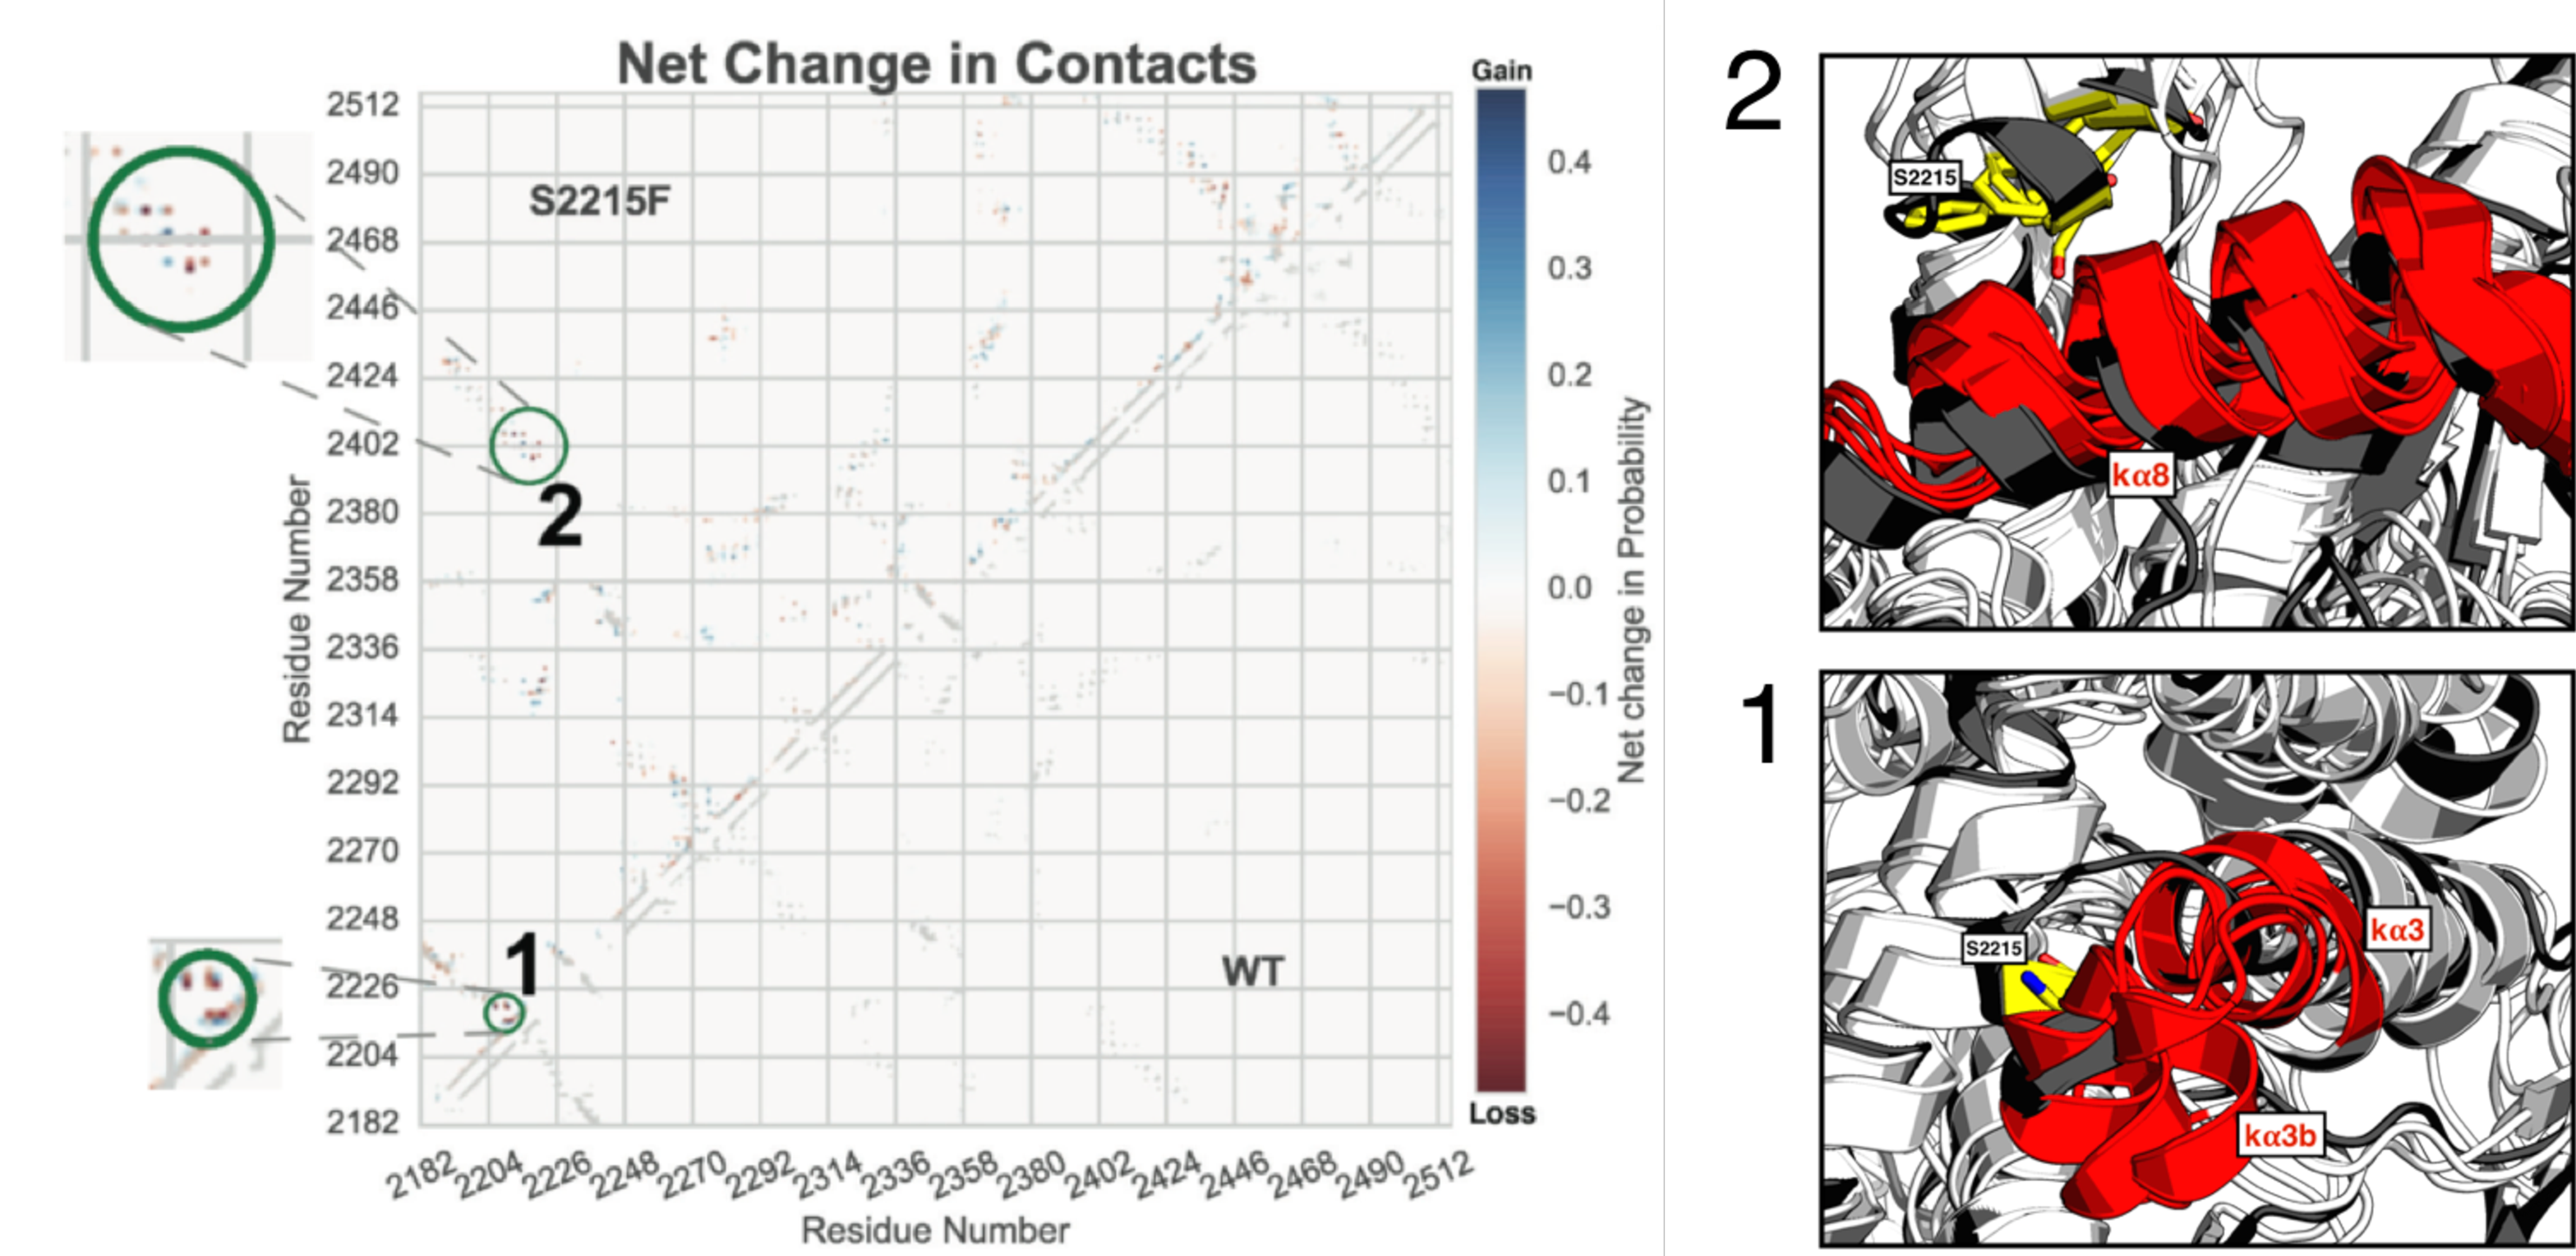
\includegraphics[width=1.0\linewidth]{figures/mtor-fig4.pdf}
		\caption[Missense mutations can perturb local structure]{
			{\bf Missense mutations can perturb local structure}
			{\bf Left} Contact map showing the difference in probability of forming a contact between WT and mutant S2215F for the kinase domain simulations. {\bf Right} Regions one and two highlighted in contact map, showing a structural perturbation in indicated helices. Starting structure is shown in gray, the residues indicated in the contact map are shown in red and residue 2215 is shown in yellow. All trajectories started from PDB: 4JSN. \bf{This left panel of this figure is a modified version of a figure that appears in~\citep{Xu:2016fw}. Reprinted with permission of James Hsieh and the Journal of Clinical investigation}
		}
		\label{fig:mtor-figure4}
	\end{figure}
\end{landscape}

\subsection{Missense mutations do not appear to shift the formation of an active kinase domain}

Despite the promise of being able to identify structural rearrangements in an automated, high-throughput fashion, contact map analysis is difficult to use to explain mechanistically how these mutants are activating. Seeking a more mechanistic understanding of how these mutants are activating, we looked at a common order parameter for activation from previous work on kinases~\citep{Shukla:2014jp}. In most kinases, there is a highly conserved lysine residue that coordinates ATP when it is bound in the active site. In mTOR, this lysine has been identified as K2187~\citep{Yang:2013gaa}. To test whether mutations are activating mTOR by shifting the kinase domain into a more active conformation, we looked at the contact formation over time between resides K2187-E2190 (indicative of an active kinase), shown in Figure~\ref{fig:mtor-figure5} in red, and E2190-R2430, shown in Figure~\ref{fig:mtor-figure5} in blue. We hypothesized that formation of the E2190-R2430 contact suggests an inactive kinase domain, as the $\alpha$C would need to rotate out and away from the active site, which has been observed in inactive kinases in previous work (Figure~\ref{fig:mtor-figure5}, inset panel)~\citep{Shukla:2014jp,Jura:2011eh}. Show on the right in Figure~\ref{fig:mtor-figure5} is a representative panel of the activating mutants from the kinase domain simulations, as well as the control wild type. While some of the mutants seem less stable than the wild type, none of them appear to shift the distribution of the kinase domain further towards formation of the K2187-E2190 contact, indicative of activation. This is likely because the mTOR kinase domain adopts an active conformation in all of the available crystal structures, and the simulations largely stay in the local minima of the crystal structure. This is further supported by the hypothesis that the mTOR kinase domain is constitutively active, and is regulated by restriction of substrate access~\citep{Yang:2013gaa,Laplante:2012fm,Saxton:2017cv}. 

\begin{landscape}
	\begin{figure}[p]
		\centering
		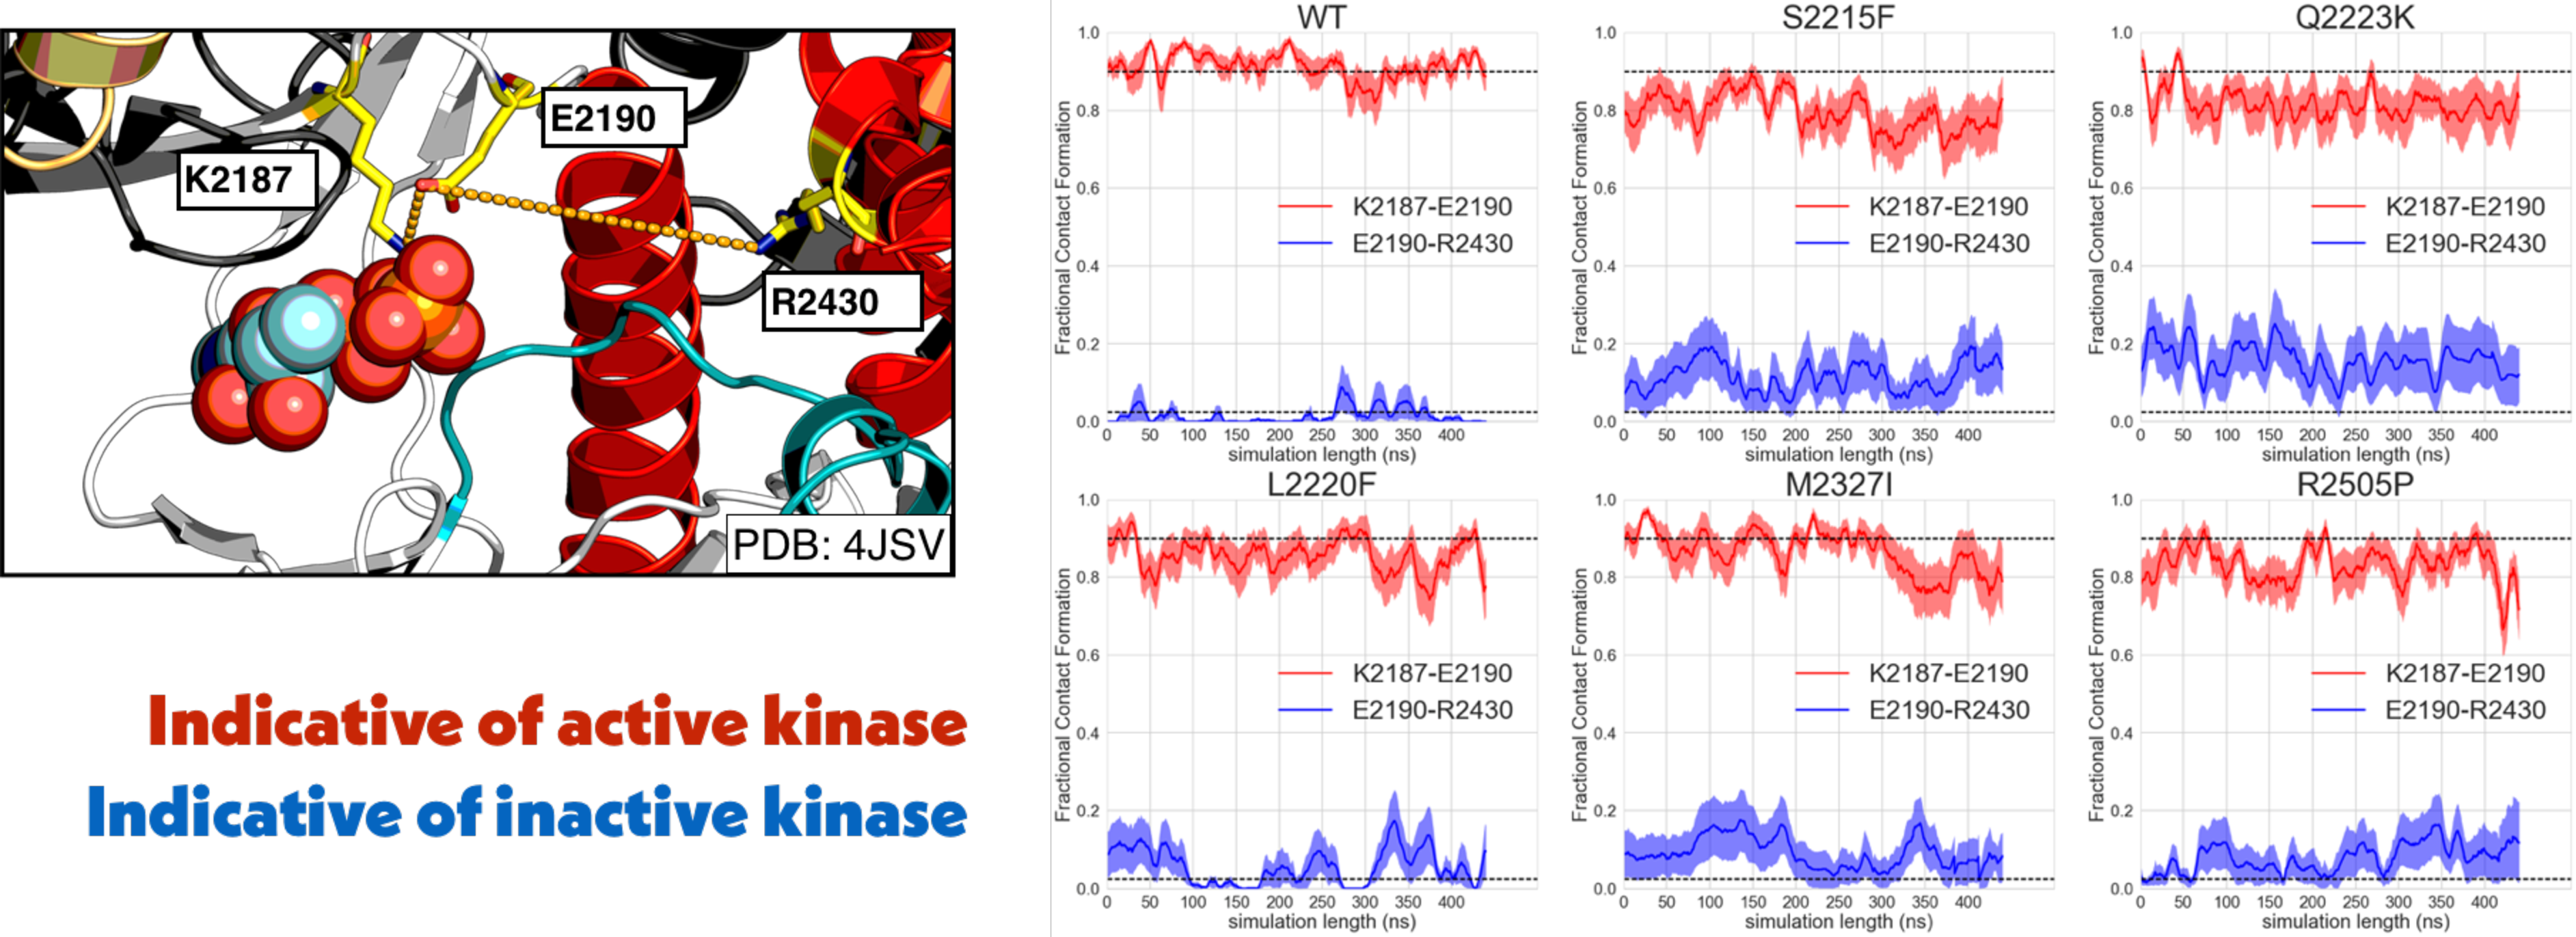
\includegraphics[width=1.0\linewidth]{figures/mtor-fig5.pdf}
		\caption[Missense mutations do not shift the population of the active conformation on a common activation order parameter]{
			{\bf Missense mutations do not shift the population of the active conformation on a common activation order parameter}
			{\bf Right} Fractional contact formation analysis for 20 500ns trajectories, analyzed in 20ns sliding window chunks. Contacts cutoff at 4Å for closest heavy atom.  Plotted is the mean $\pm$ SEM. The dashed lines represent the proportion roughly populated in the WT simulations. {\bf Left} Illustration of the bond formed between K2187 and E2190 (red) or E2190 and R2430 (blue). ATP is shown in spheres. The kinase domain (white) is shown with the activation loop (teal) and the $\alpha$ helices (red). The FRB domain is shown in gold. 
		}
		\label{fig:mtor-figure5}
	\end{figure}
\end{landscape}


\subsection{Missense mutations do not disrupt the formation of inhibitory salt bridges between the kinase and FAT domains}
Another hypothesis for how the missense mutations may be hyperactivating looked at the role the FAT domain, which clamps around the kinase domain, plays in regulating the activity of mTOR. In previous work, point mutations that disrupted the formation of the salt bridge between E2419 and R1905 (Figure~\ref{fig:mtor-figure6}, red) activated TOR signaling in yeast and mammalian cell lines~\citep{Urano:2007er}. From this observation, we hypothesized that stable contacts formed between the kinase domain and FAT domain have a negative regulatory role on the activity of mTOR, and that disruption of these bonds through some allosteric mechanism would allow an oncogenic mutant to activate mTOR. Another set of contacts, Gln1941 to Gln2200 (Figure~\ref{fig:mtor-figure6}, blue) is conserved across many mTOR orthologs~\citep{Yang:2013gaa}, suggesitng a potential regulatory role. We also looked at several other salt bridges in the vicinity of these contacts: E1147 and K2218 (cyan), Q1425 and R2322 (magenta), and E1427 and R2322 (yellow). Shown in Figure~\ref{fig:mtor-figure6} is a representative selection of mutations from the kinase domain, demonstrating that none of the salt bridges showed a prominent change from the wild type to mutant simulations. Of note, R2505P appears to have a disruption int he formation of the Q1941 and Q2200,  E1147 and K2218, and E2419 and R1905 contacts, indicating that this may be a possible mechanism of activation for this mutant. However, this is difficult to say with certainty without functional experimental data or additional computation to confirm this result. 

\begin{landscape}
	\begin{figure}[p]
		\centering
		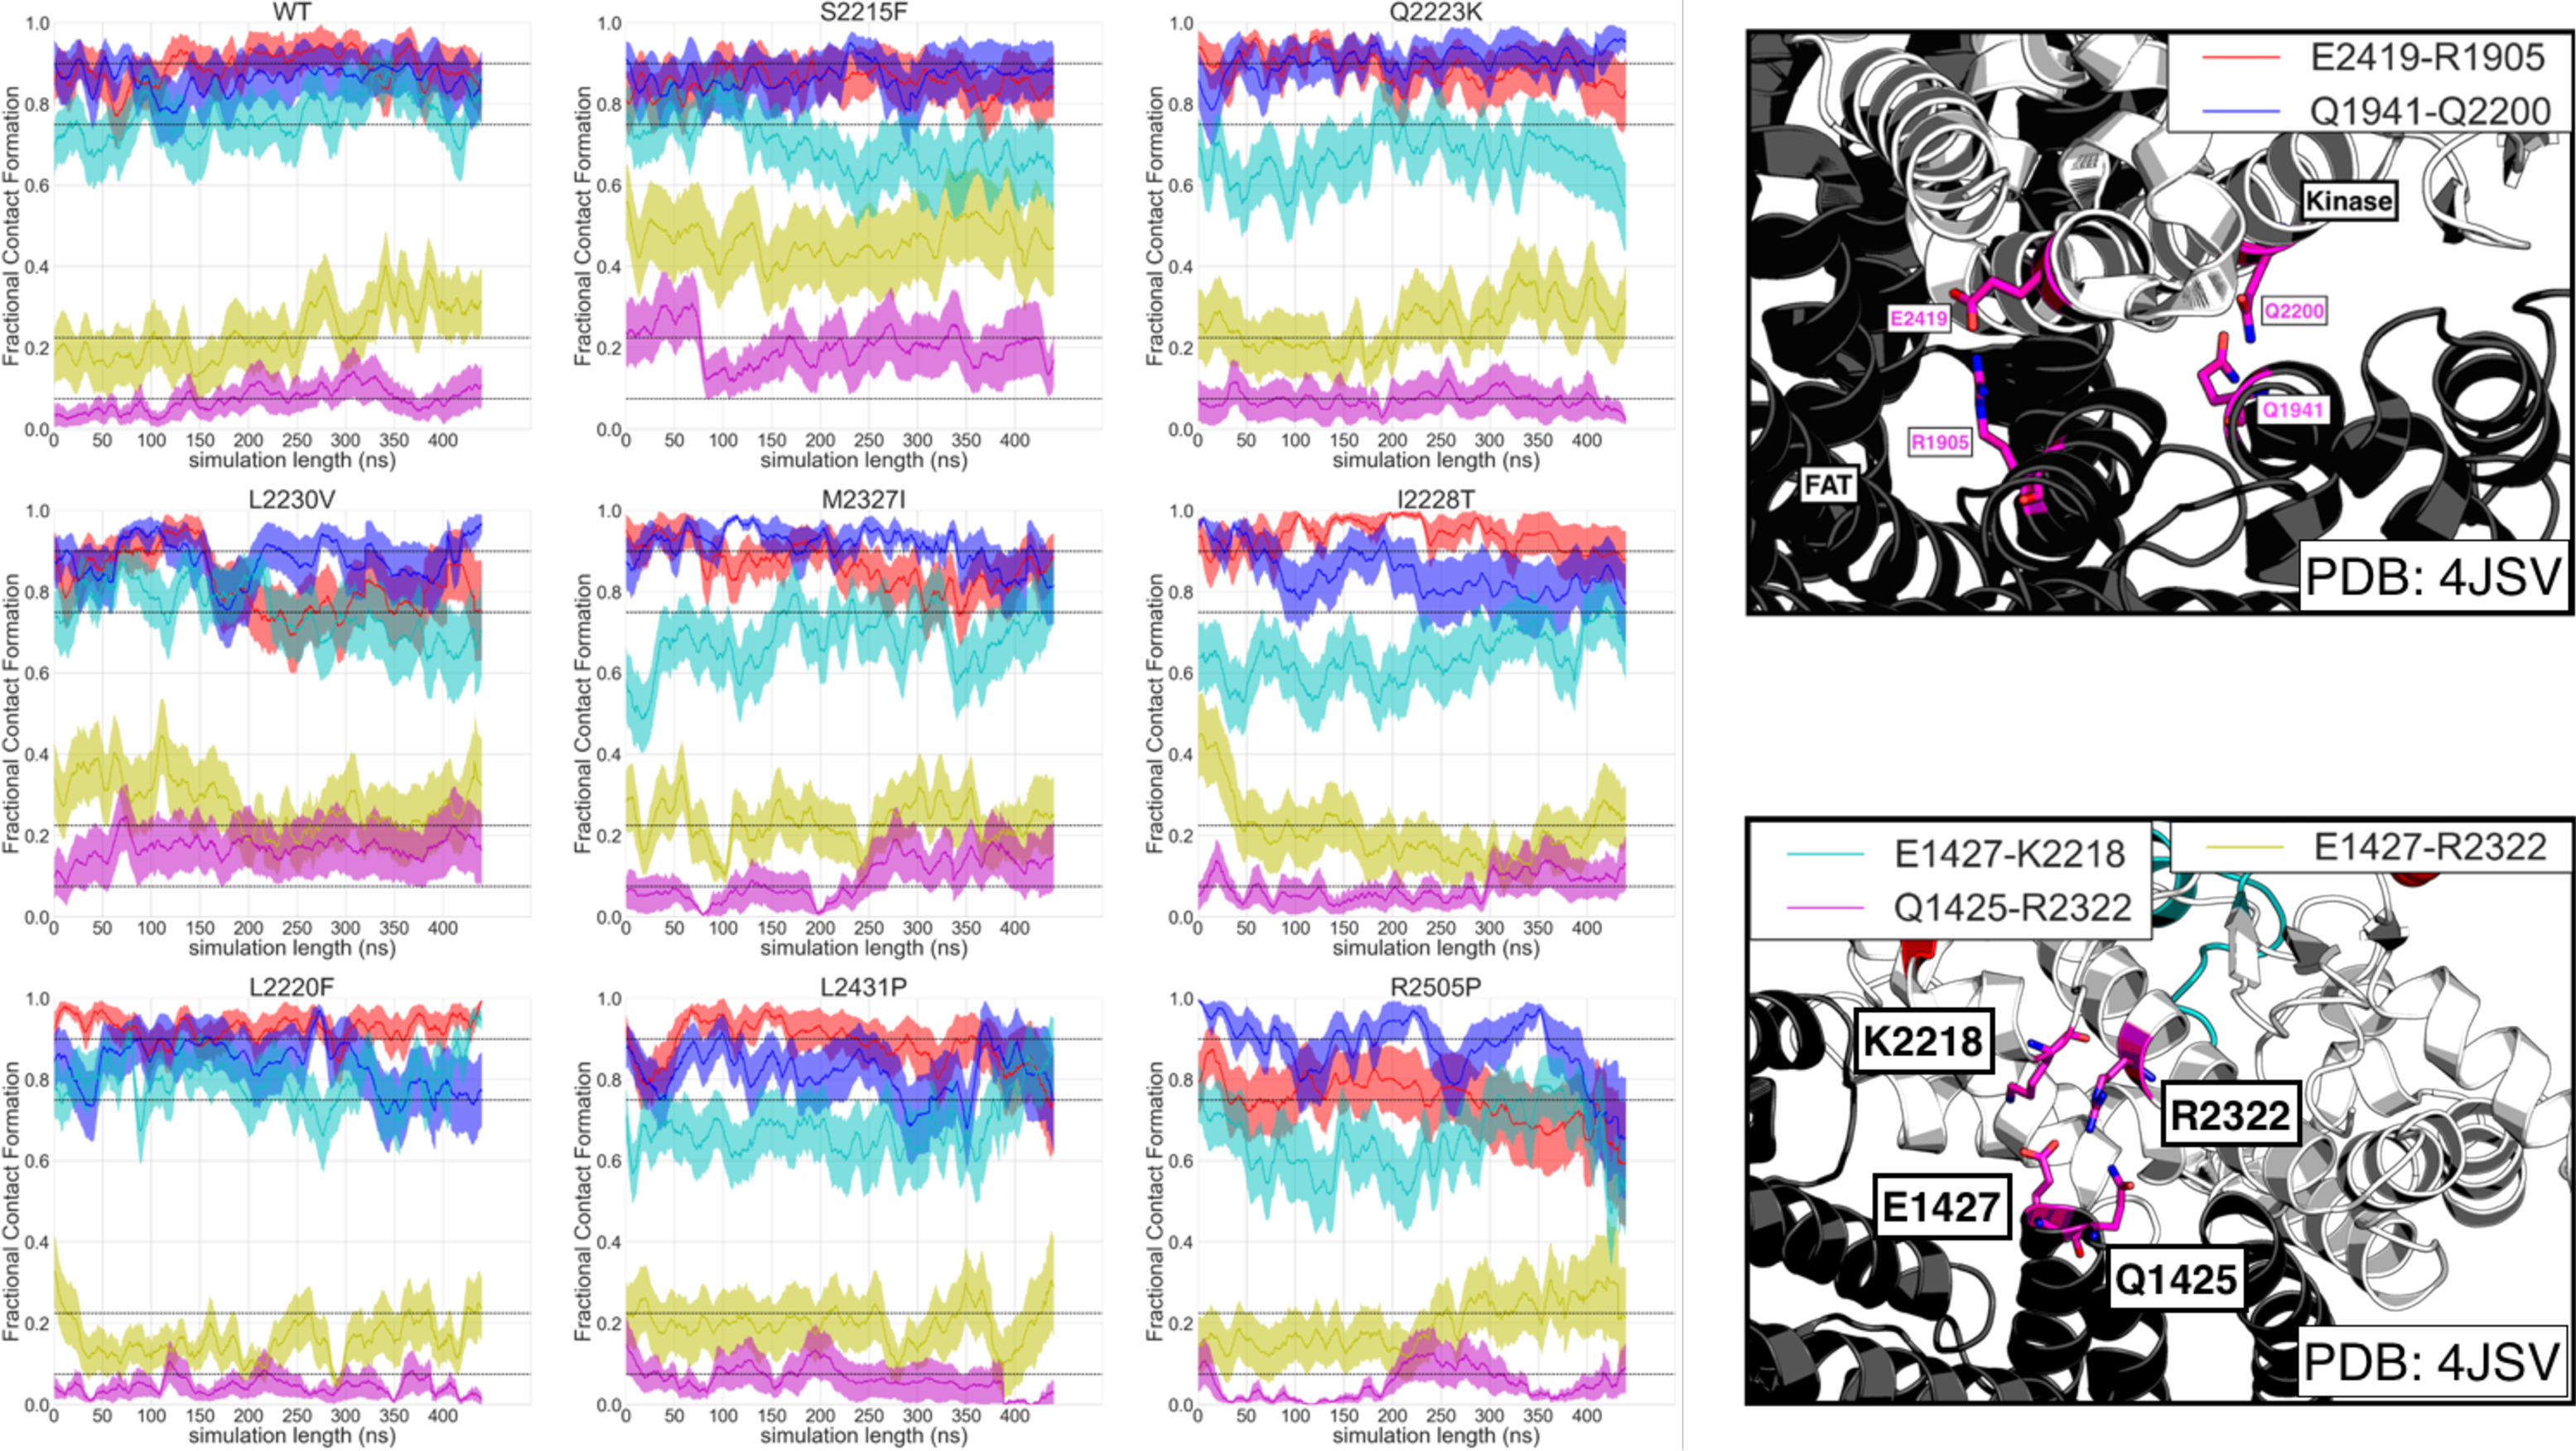
\includegraphics[width=1.0\linewidth]{figures/mtor-fig6.pdf}
		\caption[Missense mutations in kinase domain do not disrupt interactions between the kinase and FAT domains]{
			{\bf Missense mutations in kinase domain do not disrupt interactions between the kinase and FAT domains}
			{\bf Left} Fractional contact formation analysis for 10 500ns trajectories, analyzed in 20ns sliding window chunks. Contacts cutoff at 4Å for closest heavy atom.  Plotted is the mean $\pm$ SEM. The dashed lines represent the proportion roughly populated in the WT simulations. {\bf Right} Illustration of the distances being plotted between E2419 and R1905 (red), Q1941 and 2200 (blue), E1147 and K2218 (cyan), Q1425 and R2322 (magenta), or E1427 and R2322 (yellow). The kinase domain (white) interacts with the FAT domain (black) through salt bridges and hydrogen bonds formed by the highlighted residues (magenta) 
		}
		\label{fig:mtor-figure6}
	\end{figure}
\end{landscape}

\subsection{Free energy calculations show promise in predicting impact of mutations on small molecule and ATP affinity}
The preceding work on trying to understand the functional impact of mutations using traditional molecular dynamics highlights one of the key challenges of the application of physical modeling to this question: the need to compute meaningful, physically testable quantities. Alchemical free energy calculations have been previously used to predict the impact of mutations on protein-protein binding~\citep{clark2017free} and protein thermostabilities~\citep{steinbrecher2017predicting}. Based on this work, we set out to see if free energy calculations could be used to identify clinically observed mutations that might cause resistance to an ATP-competitive inhibitor. Here, we propose a model of resistance mutants that cause a decrease in affinity for an ATP-competitive inhibitor while maintaining a basic level of ATP affinity (Figure~\ref{fig:mtor-figure7}, left panels). An increase in ATP affinity could be a mechanism of resistance by making it more difficult for ATP-competitive inhibitors to out-compete ATP, as well as a mechanism of activation. To explore the impact of mutations on affinity for these compounds, we built models of mTOR bound to ATP (Figure~\ref{fig:mtor-figure7}, top left) and AZD8055 (Figure~\ref{fig:mtor-figure7}, bottom left). Using protein mutation FEP+~\citep{Hauser:2018vz,steinbrecher2017predicting}, we ran preliminary calculations for a small panel of mutations from the MSKCC-IMPACT assay~\citep{Zehir:Nat.Med.:2017}. Three showed greater than 1-log unit, or 1.4 kcal/mol, decrease in affinity for AZD8055 (Figure~\ref{fig:mtor-figure7}, blue bars). W2239C, a missense mutation observed in a patient with cervical squamous cell carcinoma that occured together with a known activating mutation S2215F~\citep{Cerami:2012eu,Gao:2013kd},  showed the greatest decrease in affinity (shown as a positive $\Delta \Delta G_{mutation}$ in Figure~\ref{fig:mtor-figure7}). While we were not able to confirm via prediction that ATP-affinity is not maintained, this result suggests that treatment with an ATP-competitive inhibitor targeting mTOR may be less effective than expected. M2345V and Y2225C are also both predicted to decrease the affinity for AZD8055. M2345V was observed in a cell line from a patient with cancer of unknown primary tissue and co-occurred with a TSC2 E75K mutation, which is likely to be loss of function~\citep{Barretina:2012fp}. Y2225C was observed in a patient with tubular stomach adenocarcinoma, who also had a slight copy number gain in both MTOR and DEPTOR~\citep{CancerGenomeAtlasResearchNetwork:2017fh}. All three of these mutations are exceedingly rare and occur in tumors with relatively high mutation burden. These preliminary results suggest that free energy calculations can potentially aid in understanding or teasing apart the functional impact of rare mutations in complex tumors.

\begin{landscape}
	\begin{figure}[p]
		\centering
		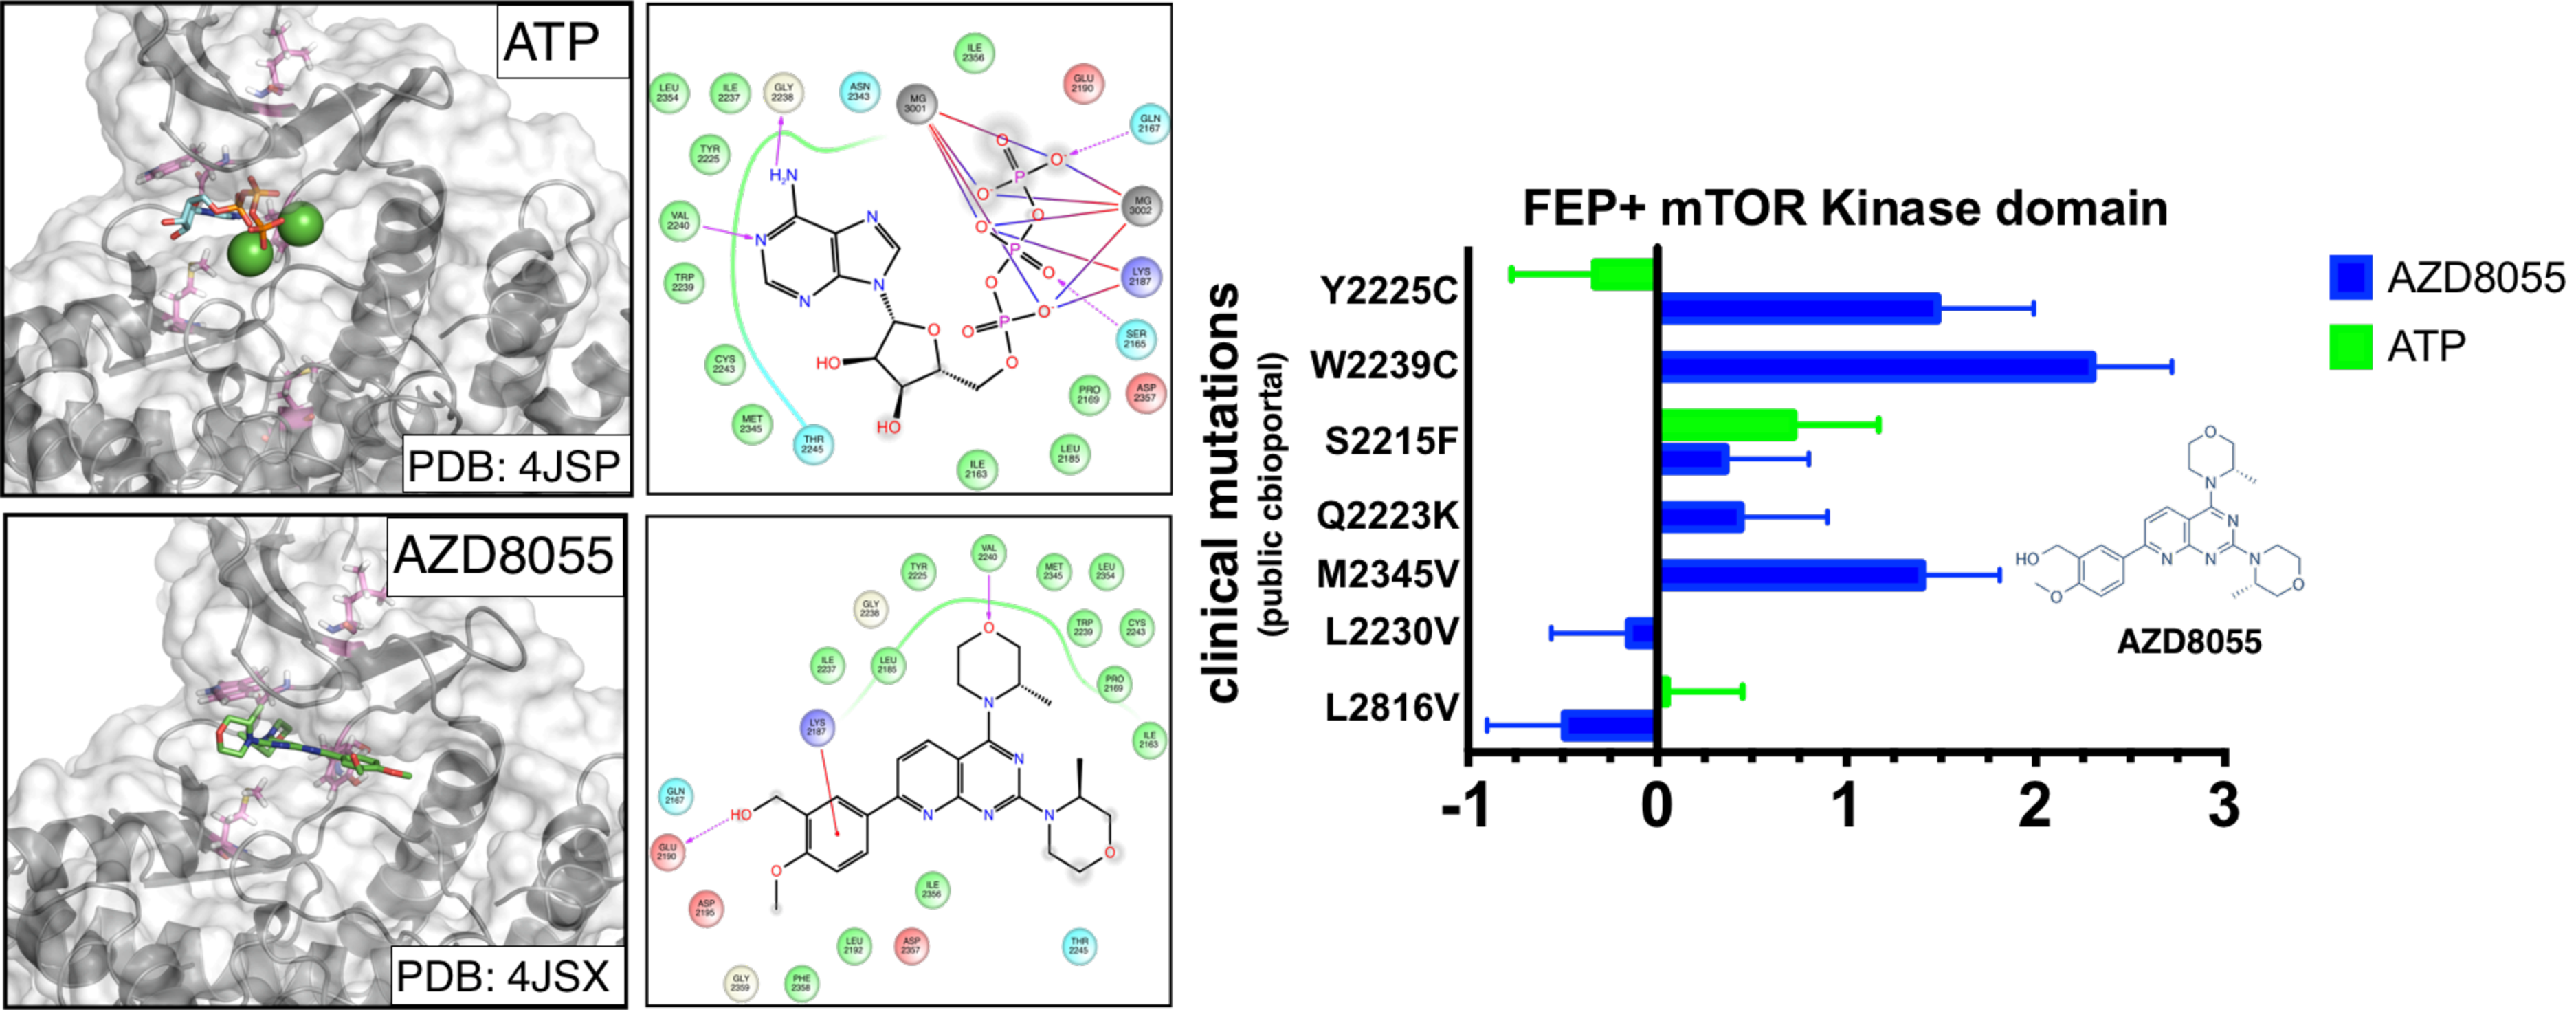
\includegraphics[width=1.0\linewidth]{figures/mtor-fig7.pdf}
		\caption[Free energy calculations identify potential resistance mutations]{
			{\bf Free energy calculations identify potential resistance mutations}
			{\bf Left} Structures and 2D interactions maps of ATP (top, PDBID: 4JSP) and AZD8055 (bottom, PDBID: 4JSX) docked to the kinase domain of mTOR. Magnesium ions are shown as green spheres.  {\bf Right} $\Delta \Delta G_{mutation}$ (x-axis) calculated for a number of clinically observed mTOR mutations(y-axis)~\citep{Zehir:Nat.Med.:2017} for ATP (green) and AZD8055 (blue). Error bars correspond to the BAR uncertainty estimate. 
		}
		\label{fig:mtor-figure7}
	\end{figure}
\end{landscape}


\section{Discussion and Conclusions}
The above work utilizes physical modeling to study the impact of clinically observed mutations on mTOR structure, function and ligand binding. mTOR is a critical node in multiple signaling pathways with a complex structure and regulatory.  Extensive molecular dynamics simulations were run on mutations that were confirmed to be hyperactivating by cellular and functional assays~\citep{Xu:2016fw}. Contact map analysis suggests that local, fast structural rearrangements are induced by mutations such as S2215F. Unfortunately, more focused studies on order parameters of activation do not yield insight into potential mechanisms of activation, suggesting that either the simulation time is insufficient to observe changes in the activation state of the kinase domain or the mechanism of activation occurs at the level of mTORC or substrate access. These studies are also limited by the relative scarcity of biophysical data for mTOR. At the time of the study, there were no atomistic structures for the mTOR complexes, impeding any study of the role mTOR mutations play in disrupting or altering the structure of the complex. Recent, exciting work using Cryo-EM has yielded a number of high resolution structures for mTORC1 and mTORC2~\citep{Yang:2017gu,Stuttfeld:2018kg,Yuan:2016ef,Yang:2016kk}. These advances would enable future work exploring the impact of mutations in the more physiologically relevant context of the complexes. Additionally, a more thorough understanding of the activation state of the mTOR crystal structure, which is assumed to be active, and what the inactive conformation of mTOR looks like would further enable these types of large scale studies. 

The challenges with using traditional MD analysis highlights the importance of looking at testable, physical surrogates for activation and resistance. Unless there are well-validated order parameters from prior experimental work to use, drawing meaningful mechanistic conclusions from computation is difficult. Here, we present a pilot study using alchemical free energy calculations to compute the impact of a small panel of clinical mutations on ATP and inhibitor affinity. Promisingly, we were able to identify three potential resistance mutations. Future work to introduce these mutations and measure binding affinities for AZD8055, as well as expanding the number of inhibitors and mutations in the dataset, could prove useful in understanding the functional impact of these mutations on treatment. Unfortunately, mTOR is a complicated and experimentally untractable system to work with, which motivated the studies presented in the next chapter of this work. 

\chapter{Predicting the impact of clinically-observed kinase mutations using physical modeling}

The work in this chapter was published in \emph{Communications Biology} as follows. 
\realsinglespacing
\flushleft{\bf Predicting resistance of clinical Abl mutations to targeted kinase inhibitors using alchemical free-energy calculations}
\flushleft{{\bf Kevin Hauser$^1$, Christopher Negron$^1$, Steven K. Albanese$^{2,3}$, Soumya Ray, Thomas Steinbrecher$^4$,  Robert Abel$^3$, John D. Chodera$^{2}$, Lingle Wang$^{3,*}$} \\
	\emph{\normalsize $^1$ Schr\"{o}dinger, New York, NY 10036} \\
	\emph{\normalsize $^2$ Louis V. Gerstner, Jr. Graduate School of Biomedical Sciences, Memorial Sloan Kettering Cancer Center, New York, NY 10065 } \\
	\emph{\normalsize $^3$ Computational and Systems Biology Program, Sloan Kettering Institute, Memorial Sloan Kettering Cancer Center, New York, NY 10065}\\
	\emph{\normalsize $^3$ Schr\"{o}dinger, GmbH, Q7 23, 68161 Mannheim, Germany} \\
	\emph{\normalsize $^*$ Corresponding Author} \\
}

\realdoublespacing
\section{Abstract}
	The therapeutic effect of targeted kinase inhibitors can be significantly reduced by intrinsic or acquired resistance mutations that modulate the affinity of the drug for the kinase.
	In cancer, the majority of missense mutations are rare, making it difficult to predict their impact on inhibitor affinity. 
	Here, we examine the potential for alchemical free-energy calculations to predict how kinase mutations modulate inhibitor affinities to Abl, a major target in chronic myelogenous leukemia (CML).
	We find these calculations can achieve useful accuracy in predicting resistance for a set of eight FDA-approved kinase inhibitors across 144 clinically-identified point mutations, achieving a root mean square error in binding free energy changes of $1.1_{0.9}^{1.3}$ kcal mol$^{-1}$ (95\% confidence interval) and correctly classifying mutations as resistant or susceptible with $88_{82}^{93}$\% accuracy.
	This benchmark establishes the potential for physical modeling to collaboratively support the assessment and anticipation of patient mutations to affect drug potency in clinical applications.
	
\section{Introduction}

Targeted kinase inhibitors are a major therapeutic class in the treatment of cancer.
A total of 38 selective small molecule kinase inhibitors have now been approved by the FDA~\citep{fda-approved-kinase-inhibitors}, including 34 approved to treat cancer, and perhaps 50\% of all current drugs in development target kinases~\citep{Santos:Nat.Rev.DrugDiscov.:2016}.
Despite the success of selective inhibitors, the emergence of drug resistance remains a challenge in the treatment of cancer~\citep{Shah:CancerCell:2002,BUCZEK201431,huang2015mechanisms,Meyer2051,Davare29092015,VanAllen94,Rani3821,Holohan:Nat.Rev.Cancer:2013} and has motivated the development of second- and then third-generation inhibitors aimed at overcoming recurrent resistance mutations~\citep{Weisberg:Nat.Rev.Cancer:2007,Y.Lu:Curr.Med.Chem.:2011,Juchum:DrugResist.Updat.:2015,Song:ActaPharm.Sin.B:2015,Neel:NpjPrecis.Oncol.:2017}.   

While a number of drug resistance mechanisms have been identified in cancer (e.g., induction of splice variants~\citep{Gruber2006}, or alleviation of feedback~\citep{Chandarlapaty:CancerCell:2011}), inherent or acquired missense mutations in the kinase domain of the target of therapy are a major form of resistance to tyrosine kinase inhibitors (TKI)~\citep{Knight:Nat.Rev.Cancer:2010,Holohan:Nat.Rev.Cancer:2013,Housman:Cancers:2014}.
Oncology is entering a new era with major cancer centers now deep sequencing tumors to reveal genetic alterations that may render subclonal populations susceptible or resistant to targeted inhibitors~\citep{Zehir:Nat.Med.:2017}, but the use of this information in precision medicine has lagged behind. 
It would be of enormous value in clinical practice if an oncologist could reliably ascertain whether these mutations render the target of therapy resistant or susceptible to available inhibitors; such tools would facilitate the enrollment of patients in mechanism-based basket trials~\citep{Redig::2015,Hyman:Cell:2017}, help prioritize candidate compounds for clinical trials, and aid the development of next-generation inhibitors. 

\subsection{The long tail of rare kinase mutations frustrates prediction of drug resistance}
While some cancer missense mutations are highly recurrent and have been characterized clinically or biochemically, a long tail of rare mutations collectively accounts for the majority of clinically observed missense mutations (Figure ~\ref{fig:abl-figure1}A), leaving clinicians and researchers without knowledge of whether these uncharacterized mutations might lead to resistance.
While rules-based and machine learning schemes are still being assessed in oncology contexts, work in predicting drug response to microbial resistance has shown that rare mutations present a significant challenge to approaches that seek to predict resistance to therapy~\citep{Pesesky:Front.Microbiol.:2016}.
Clinical cancer mutations may impact drug response through a variety of mechanisms by altering kinase activity, ATP affinity, substrate specificities, and the ability to participate in regulatory interactions, compounding the difficulties associated with limited datasets that machine learning approaches face.
In parallel with computational approaches, high-throughput experimental techniques such as MITE-Seq~\citep{Melnikov:NucleicAcidsRes.:2014} have been developed to assess the impact of point mutations on drug response. 
However, the complexity of defining selection schemes that reliably correlate with \emph{in vivo} drug effectiveness and long turn-around times might limit their ability to rapidly and reliably impact clinical decision-making.	

\begin{landscape}
	\begin{figure}[p]
		\centering
		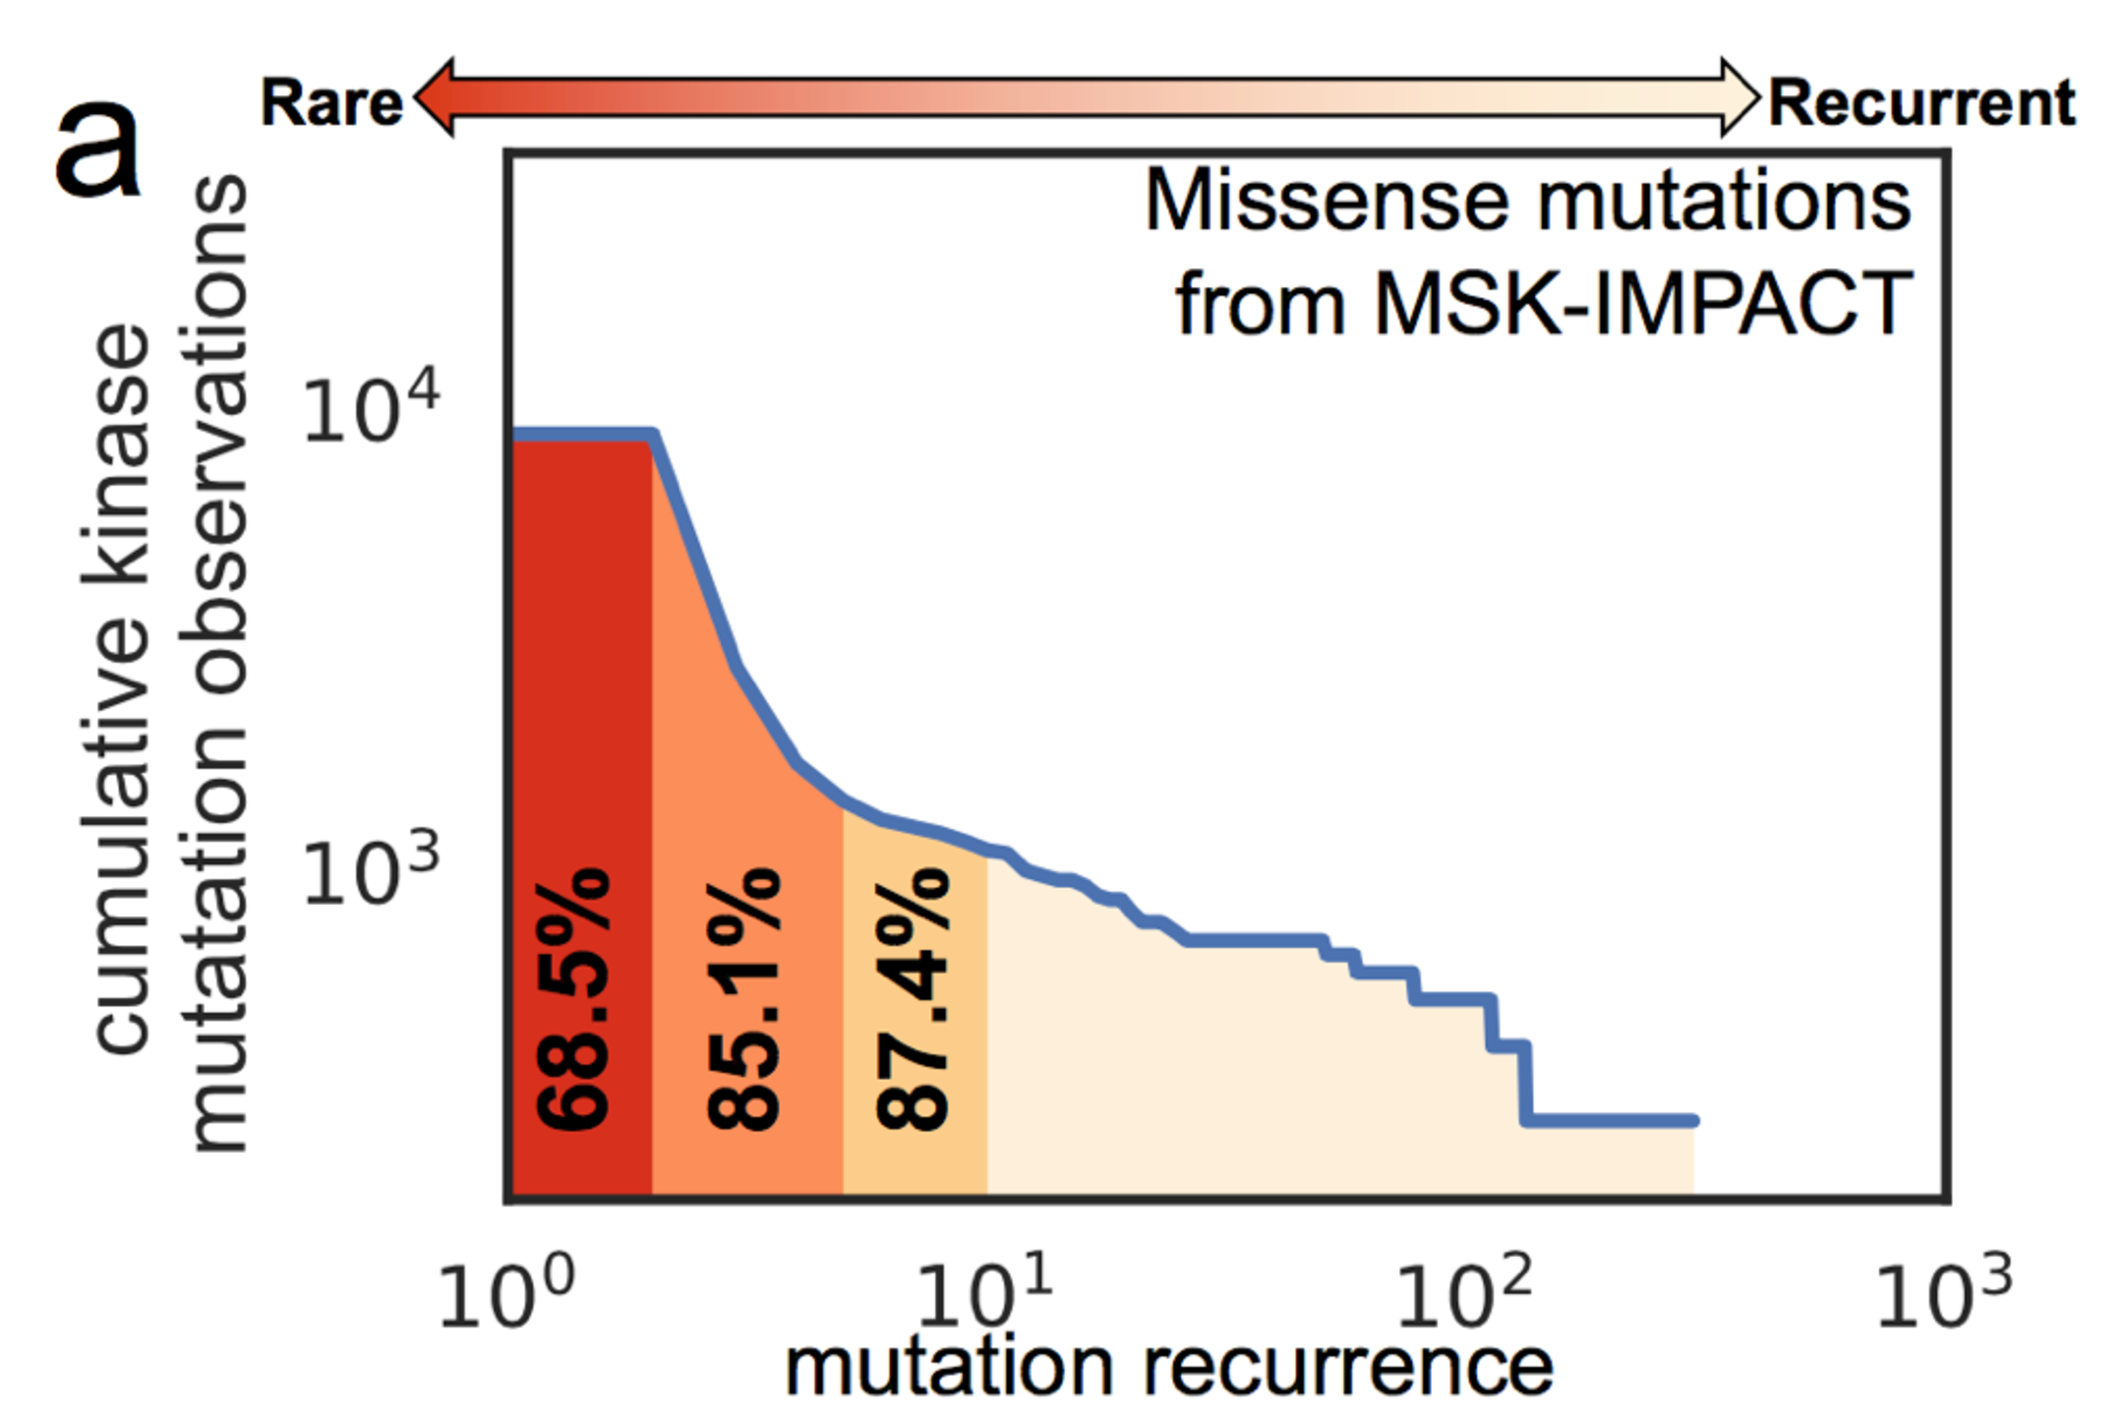
\includegraphics[width=0.8\linewidth]{figures/abl-figure-1.pdf}
		\caption[Relative alchemical free-energy calculations can be used to predict affinity changes of FDA-approved selective kinase inhibitors arising from clinically-identified mutations in their targets of therapy.]{
			{\bf Relative alchemical free-energy calculations can be used to predict affinity changes of FDA-approved selective kinase inhibitors arising from clinically-identified mutations in their targets of therapy.}
			\emph{(a)}
			Missense mutation statistics derived from 10,336 patient samples subjected to Memorial Sloan
			Kettering-Integrated Mutation Profiling of Actionable Cancer Targets (MSK-IMPACT) deep sequencing panel~\citep{Zehir:Nat.Med.:2017} show that 68.5\% of missense kinase mutations in cancer patients have never been observed previously, while 87.4\% have been observed no more than ten times; the vast majority of clinically observed missense kinase mutations are unique to each patient.
			\emph{(b)} To compute the impact of a clinical point mutation on inhibitor binding free energy, a thermodynamic cycle can be used to relate the free energy of the wild-type and mutant kinase in the absence (top) and presence (bottom) of the inhibitor.
			\emph{(c)} Summary of mutations studied in this work. 
			Frequency of the wild-type (dark green) and mutant (green) residues for the 144 clinically-identified Abl mutations used in this study (see \TABLE{table-1} for data sources). 
			Also shown is the frequency of residues within 5 {\AA} (light blue) and 8 {\AA} (blue) of the binding pocket. 
			The ordering of residues along the x-axis corresponds to the increasing occurrence of residues within 5 {\AA} of the binding pocket.
			The number of wild-type Phe residues (n=45) and mutant Val residues (n=31) exceeded the limits of the y-axis.
		}
		\label{fig:abl-figure1}
	\end{figure}
\end{landscape}

\subsection{Alchemical free-energy methods can predict inhibitor binding affinities}
Physics-based approaches could be complementary to machine-learning and experimental techniques in predicting changes in TKI affinity due to mutations with few or no prior clinical observations.
Modern atomistic molecular mechanics forcefields such as OPLS3~\citep{Harder:J.Chem.TheoryComput.:2016}, CHARMM~\citep{Huang:J.Comput.Chem.:2013}, and AMBER FF14SB~\citep{Maier:J.Chem.TheoryComput.:2015} have reached a sufficient level of maturity to enable the accurate and reliable prediction of receptor-ligand binding free energy.
Alchemical free-energy methods permit receptor-ligand binding energies to be computed rigorously, including all relevant entropic and enthalpic contributions~\citep{Chodera:Curr.Opin.Struct.Biol.:2011}.
Encouragingly, kinase:inhibitor binding affinities have been predicted using alchemical free-energy methods with mean unsigned errors of 1.0 kcal mol$^{-1}$ for CDK2, JNK1, p38, and Tyk2~\citep{Wang:J.Am.Chem.Soc.:2015,abel2017accelerating}.
Beyond kinases, alchemical approaches have predicted the binding affinity of BRD4 inhibitors with mean absolute errors of 0.6 kcal mol$^{-1}$~\citep{Aldeghi:ChemSci:2016}.
Alchemical methods have also been observed to have good accuracy (0.6 kcal mol$^{-1}$ mean unsigned error for Tyk2 tyrosine kinase) in the prediction of relative free energies for ligand transformations within a complex whose receptor geometry was generated using a homology model~\citep{cappel2016}.

%Protein-alchemical free energy results
\subsection{Alchemical approaches can predict the impact of protein mutations on free energy}
Alchemical free-energy calculations have also been used to predict the impact of mutations on protein-protein binding~\citep{clark2017free} and protein thermostabilities~\citep{steinbrecher2017predicting}.
Recent work has found that protein mutations can be predicted to be stabilizing or destabilizing with a classification accuracy of 71\% across ten proteins and 62 mutations ~\citep{Ford:J.Chem.Inf.Model.:2017}.  
The impact of Gly to D-Ala mutations on protein stability was predicted using an alchemical approach with a similar level of accuracy~\citep{Zou:J.Am.Chem.Soc.:2016}.
Recently, one study has hinted at the potential utility of alchemical free-energy calculations in oncology by predicting the impact of a single clinical mutation on the binding free energies of the TKIs dasatinib and RL45~\citep{mondal2016}.



\subsection{Assessing the potential for physical modeling to predict resistance to FDA-approved TKIs}
Here, we ask whether physical modeling techniques may be useful in predicting whether clinically-identified kinase mutations lead to drug resistance or drug sensitivity.
We perform state-of-the-art relative alchemical free-energy calculations using FEP+~\citep{Wang:J.Am.Chem.Soc.:2015}, recently demonstrated to achieve sufficiently good accuracy to drive the design of small-molecule inhibitors for a broad range of targets during lead optimization~\citep{Lovering:ChemMedChem:2016,Chodera:Curr.Opin.Struct.Biol.:2011,Wang:J.Am.Chem.Soc.:2015,abel2017accelerating}, to calculate the effect of point mutation on the binding free energy between the inhibitor and the kinase receptor (\FIG{figure-1}b).
Figure~\ref{fig:abl-figure1}B depicts the thermodynamic cycle that illustrates how we used relative free energy calculations to compute the change in ligand binding free energy in response to the introduction of a point mutation in the kinase (Figure~\ref{fig:abl-figure1}C).
We compare this approach against a fast but approximate physical modeling method implemented in Prime~\citep{Rapp:J.Chem.Inf.Model.:2011} (an MM-GBSA approach) in which an implicit solvent model is used to assess the change in minimized interaction energy of the ligand with the mutant and wild-type kinase.
We consider whether these methods can predict a ten-fold reduction in inhibitor affinity (corresponding to a binding free energy change of 1.36 kcal mol$^{-1}$) to assess baseline utility.
As a benchmark, we compile a set of reliable inhibitor $\Delta$pIC$_{50}$ data for 144 clinically-identified mutants of the human kinase Abl, an important oncology target dysregulated in cancers like chronic myelogenous leukemia (CML), for which six~\citep{fda-approved-kinase-inhibitors} FDA-approved TKIs are available.
While $\Delta$pIC$_{50}$ can approximate a dissociation constant $\Delta K_{D}$, other processes contributing to changes in cell viability might affect IC$_{50}$ in ways that are not accounted for by a traditional binding experiment, motivating a quantitative comparison between $\Delta$pIC$_{50}$ and $\Delta K_{D}$.
The results of this benchmark demonstrate the potential for FEP+ to predict the impact that mutations in Abl kinase have on drug binding, and a classification accuracy of $88_{82}^{93}$\%  (for all statistical metrics reported in this paper, the 95\% confidence intervals (CI) is shown in the form of ($x^{upper}_{lower}$)), an RMSE of $1.07_{0.89}^{1.26}$ kcal mol$^{-1}$, and an MUE of $0.79_{0.67}^{0.92}$ kcal mol$^{-1}$ was achieved. 

\section{Results}
\subsection{A benchmark of $\Delta$pIC$_{50}$s for predicting mutational resistance} 
To construct a benchmark evaluation dataset, we compiled a total of 144  $\Delta$pIC$_{50}$ measurements of Abl:TKI affinities, summarized in \TABLE{table-1}, taking care to ensure all measurements for an individual TKI were reported in the same study from experiments run under identical conditions.
131 $\Delta$pIC$_{50}$ measurements were available across the six TKIs with available co-crystal structures with wild-type Abl---26 for axitinib and 21 for bosutinib, dasatinib, imatinib, nilotinib, and ponatinib.
13 $\Delta$pIC$_{50}$ measurements were available for the two TKIs for which docking was necessary to generate Abl:TKI structures---7 for erlotinib and 6 for gefitinib. 
For added diversity, this set includes TKIs for which Abl is not the primary target---axitinib, erlotinib, and gefitinib.
All mutations in this benchmark dataset have been clinically-observed (Supplementary Table \ref{tab:abl-table-si-1}). Due to the change in bond topology required by mutations involving proline, which is not currently supported by the FEP+ technology for protein residue mutations, the three mutations H396P (axitinib, gefitinib, erlotinib) were excluded from our assessment. As single point mutations were highly represented in the Memorial Sloan
Kettering-Integrated Mutation Profiling of Actionable Cancer Targets (MSK-IMPACT) study analyzed in Figure~\ref{fig:abl-figure1}A, we excluded double mutations from this work. However, the impact of mutations from multiple sites can potentially be modeled by sequentially mutating each site and this will be addressed in future work.

\begin{landscape}
\begin{table}[bt]
	\caption[ Public $\Delta$pIC$_{50}$ datasets for 144 Abl kinase mutations and eight tyrosine kinase inhibitors (TKIs) with corresponding wild-type co-crystal structures used in this study]{
		\label{tab:abl-table-1}
		{\bf Public $\Delta$pIC$_{50}$ datasets for 144 Abl kinase mutations and eight tyrosine kinase inhibitors (TKIs) with corresponding wild-type co-crystal structures used in this study}
	}
	% Use "S" column identifier to align on decimal point 
	\setlength{\tabcolsep}{4pt}
	\begin{tabularx}{\textwidth}{X c c X X S S S}
		\toprule
		&				 		&			& 			&				& {(kcal mol$^{-1}$)}  										&										& {(kcal mol$^{-1}$)}		\\
		{\bf TKI}	& {\bf N}$_\mathrm{mut}$& {\bf R}	& {\bf S}	& {\bf PDB}		& {$|\Delta G_\mathrm{max} - \Delta G_\mathrm{min}|$}	& {\bf Source}							& {$\Delta G_\mathrm{WT}$} \\
		\toprule
		axitinib	& 26					& 0			& 26		& 4wa9          & 2.05    												& \cite{Pemovska:Nature:2015}			& -8.35		\\
		bosutinib	& 21					& 4			& 17		& 3ue4         	& 2.79    												& \cite{Gozgit3992}						& -9.81		\\
		dasatinib	& 21					& 5			& 16		& 4xey        	& 5.08    												& \cite{Gozgit3992}						& -11.94	\\
		imatinib	& 21					& 5			& 16		& 1opj          & 2.16    												& \cite{Gozgit3992} 					& -9.19		\\
		nilotinib	& 21					& 4			& 17		& 3cs9       	& 3.88    												& \cite{Gozgit3992} 					& -10.74	\\
		ponatinib	& 21					& 0			& 21		& 3oxz        	& 1.00    												& \cite{Gozgit3992} 					& -11.70	\\
		%
		{\bf subtotal}& {\bf 131}			&{\bf 18}	&{\bf 113}	& 				& 	    												& 										&	\\
		%
		erlotinib	& 7 					& 1			& 6			& \it{Dock to 3ue4}	& 1.73    												& \cite{Davis:Nat.Biotechnol.:2011}		& -9.77		\\
		gefitinib	& 6						& 0			& 6			& \it{Dock to 3ue4}	& 1.79    												& \cite{Davis:Nat.Biotechnol.:2011}		& -8.84		\\
		%
		{\bf total}	& {\bf 144}				&{\bf 19}	&{\bf 125}	& 				&														&										& 	\\
		\bottomrule
	\end{tabularx}
	\small
	\smallskip
	\\
	{\bf N}$_\mathrm{mut}$: Total number of mutants for which $\Delta$pIC$_{50}$ data was available.\\
	Number of {\bf R}esistant, {\bf S}usceptical mutants using 10-fold affinity change threshold.\\
	PDB: Source PDB ID, or \emph{Dock to 3ue4}, which used 3ue4 as the receptor for Glide-SP docking inhibitors without co-crystal structure.\\
	$\Delta G_\mathrm{WT}$: Binding free energy of inhibitor to wild-type Abl, as estimated from IC$_{50}$ data.
\end{table}
\end{landscape}

Experimental $\Delta$pIC$_{50}$ measurements for wild-type and mutant Abl were converted to $\Delta\Delta$G in order to make direct comparisons between physics-based models and experiment.
However, computation of experimental uncertainties were required to understand the degree to which differences between predictions and experimental data were significant.
Since experimental error estimates for measured IC$_{50}$s were not available for the data in Table~\ref{tab:abl-table-1}, we compared that data to other sources that have published IC$_{50}$s for the same mutations in the presence of the same TKIs (Figure~\ref{fig:abl-figure2}A,B,C).
Cross-comparison of 97 experimentally measured $\Delta\Delta$Gs derived from cell viability assay IC$_{50}$ data led to an estimate of experimental variability of $0.32^{0.36}_{0.28}$ kcal mol$^{-1}$ root-mean square error (RMSE) that described the expected repeatability of the measurements.
Because multiple factors influence the IC$_{50}$ aside from direct effects on the binding affinity---the focus of this study---we also compared $\Delta\Delta$Gs derived from $\Delta$pIC$_{50}$s with those derived from binding affinity measurements ($\Delta K_{d}$) for which data for a limited set of 27 mutations was available (Figure~\ref{fig:abl-figure2}D); the larger computed RMSE of $0.81^{1.04}_{0.59}$ kcal mol$^{-1}$ represents an estimate of the lower bound of the RMSE to the IC$_{50}$-derived $\Delta\Delta$Gs that we might hope to achieve with FEP+ or Prime, which were performed using non-phosphorylated models, when comparing sample statistics directly.
In comparing 31 mutations for which phosphorylated and non-phosphorylated $\Delta K_{d}$s were available, we found a strong correlation between the $\Delta\Delta$Gs derived from those data (r=0.94, Figure \ref{fig:abl-figure-si-1}); the statistics of that comparison are similar to those of the inter-lab variability comparison.

\begin{landscape}
	\begin{figure}[p]
		\centering
		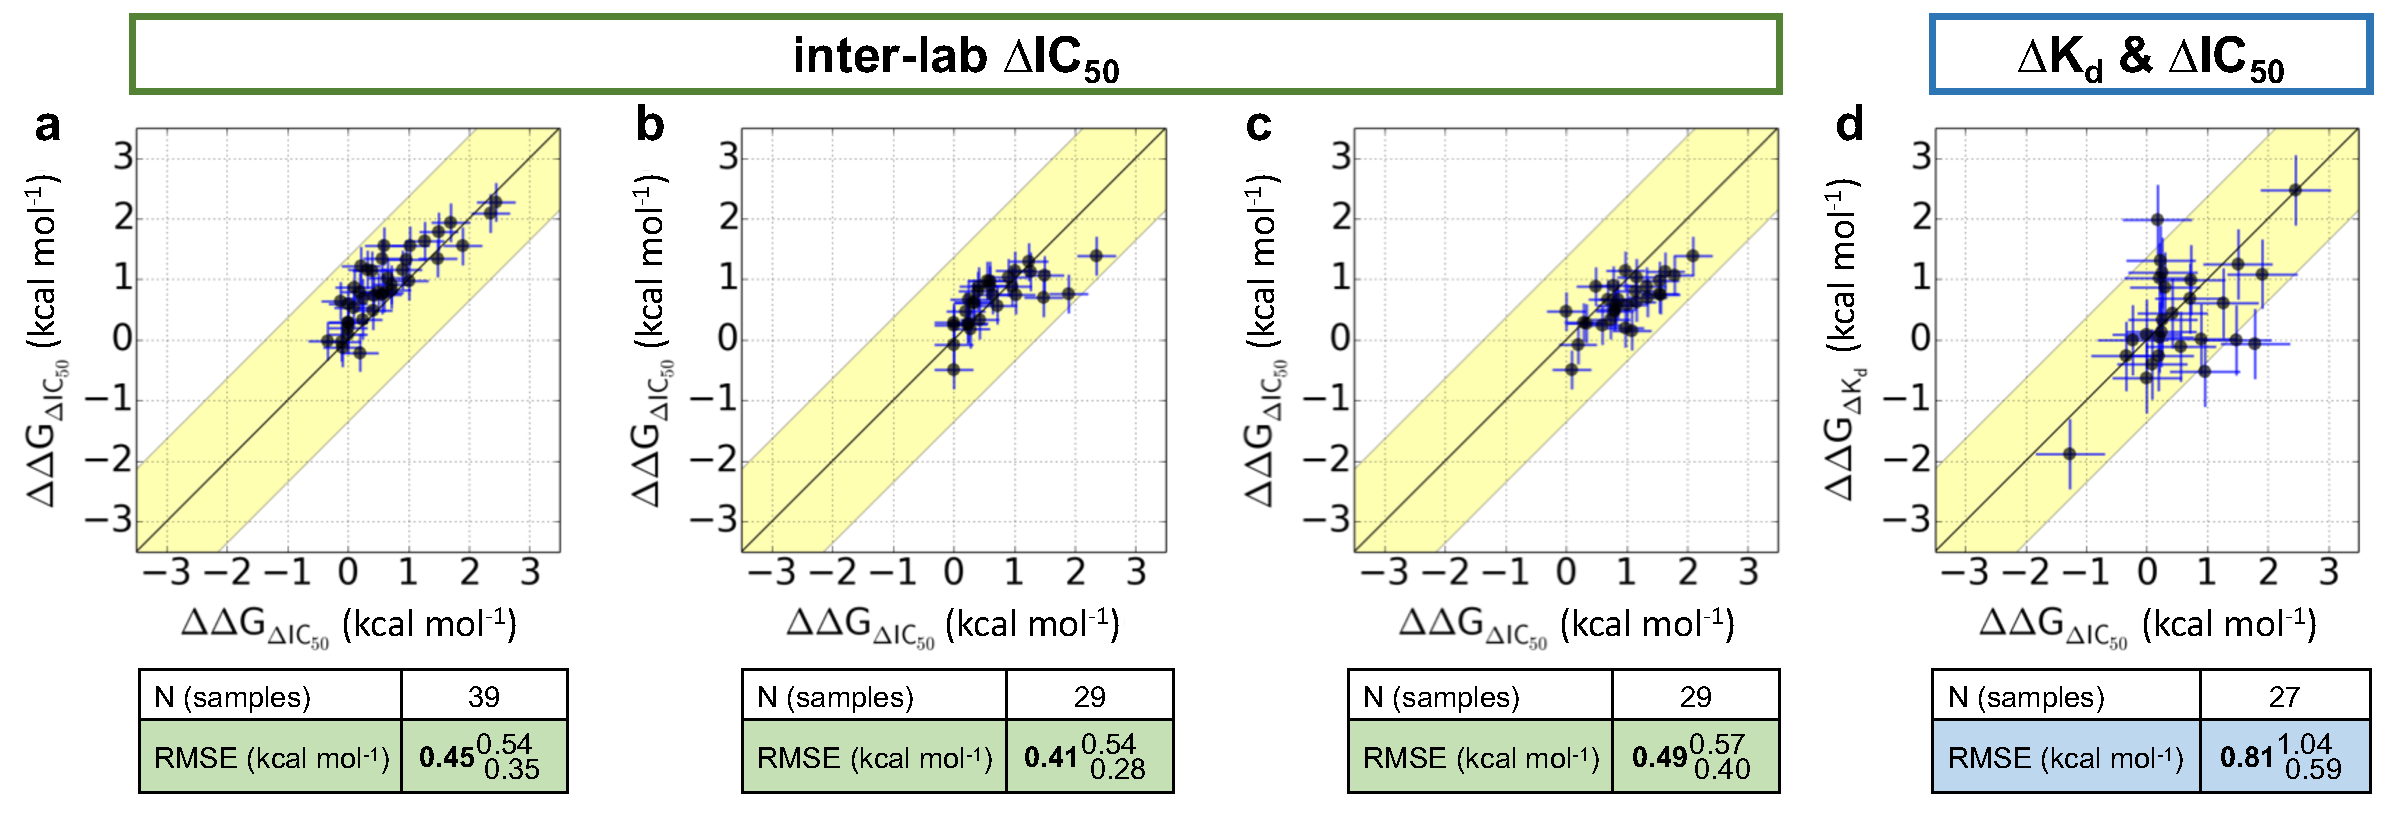
\includegraphics[width=0.8\linewidth]{figures/abl-figure-2.pdf}
		\caption[Cross-comparison of the experimentally measured effects that mutations in Abl kinase have on ligand binding, performed by different labs.]{
		{\bf Cross-comparison of the experimentally measured effects that mutations in Abl kinase have on ligand binding, performed by different labs.}
		$\Delta\Delta$G was computed from publicly available $\Delta$pIC$_{50}$ or $\Delta$p$K_{d}$ measurements and these values of $\Delta\Delta$G were then plotted and the RMSE between them reported.
		({\bf a}) $\Delta$pIC$_{50}$ measurements (X-axis) from \protect\cite{Gozgit3992} compared with $\Delta$pIC$_{50}$ measurements (Y-axis) from \protect\cite{Soverini7374}.
		({\bf b}) $\Delta$pIC$_{50}$ measurements (X-axis) from \protect\cite{Gozgit3992} compared with $\Delta$pIC$_{50}$ measurements (Y-axis) from \protect\cite{o2007bcr}.
		({\bf c}) $\Delta$pIC$_{50}$ measurements (X-axis) from \protect\cite{Soverini7374} compared with $\Delta$pIC$_{50}$ measurements (Y-axis) from \protect\cite{o2007bcr}.
		({\bf d}) $\Delta$pIC$_{50}$ measurements (X-axis) from \protect\cite{Gozgit3992} compared with $\Delta$p$K_{d}$ measurements (Y-axis) from \protect\cite{Davis:Nat.Biotechnol.:2011} using non-phosphorylated Abl kinase.
		Scatter plot error bars in a,b,and c are $\pm$standard error (SE) taken from the combined 97 inter-lab $\Delta\Delta$Gs derived from the $\Delta$pIC$_{50}$ measurements, which was 0.32$_{0.28}^{0.36}$;
		the RMSE was 0.45$_{0.39}^{0.51}$ kcal mol$^{-1}$. Scatter plot error bars in d are the $\pm$standard error (SE) of $\Delta\Delta$Gs derived from $\Delta$pIC$_{50}$ and $\Delta$p$K_{d}$ from a set of 27 mutations, which is 0.58$_{0.42}^{0.74}$ kcal mol$^{-1}$;
		the RMSE was 0.81$_{0.59}^{1.04}$ kcal mol$^{-1}$.
	}
		\label{fig:abl-figure2}
	\end{figure}
\end{landscape}

\begin{landscape}
	\begin{figure}[p]
		\centering
		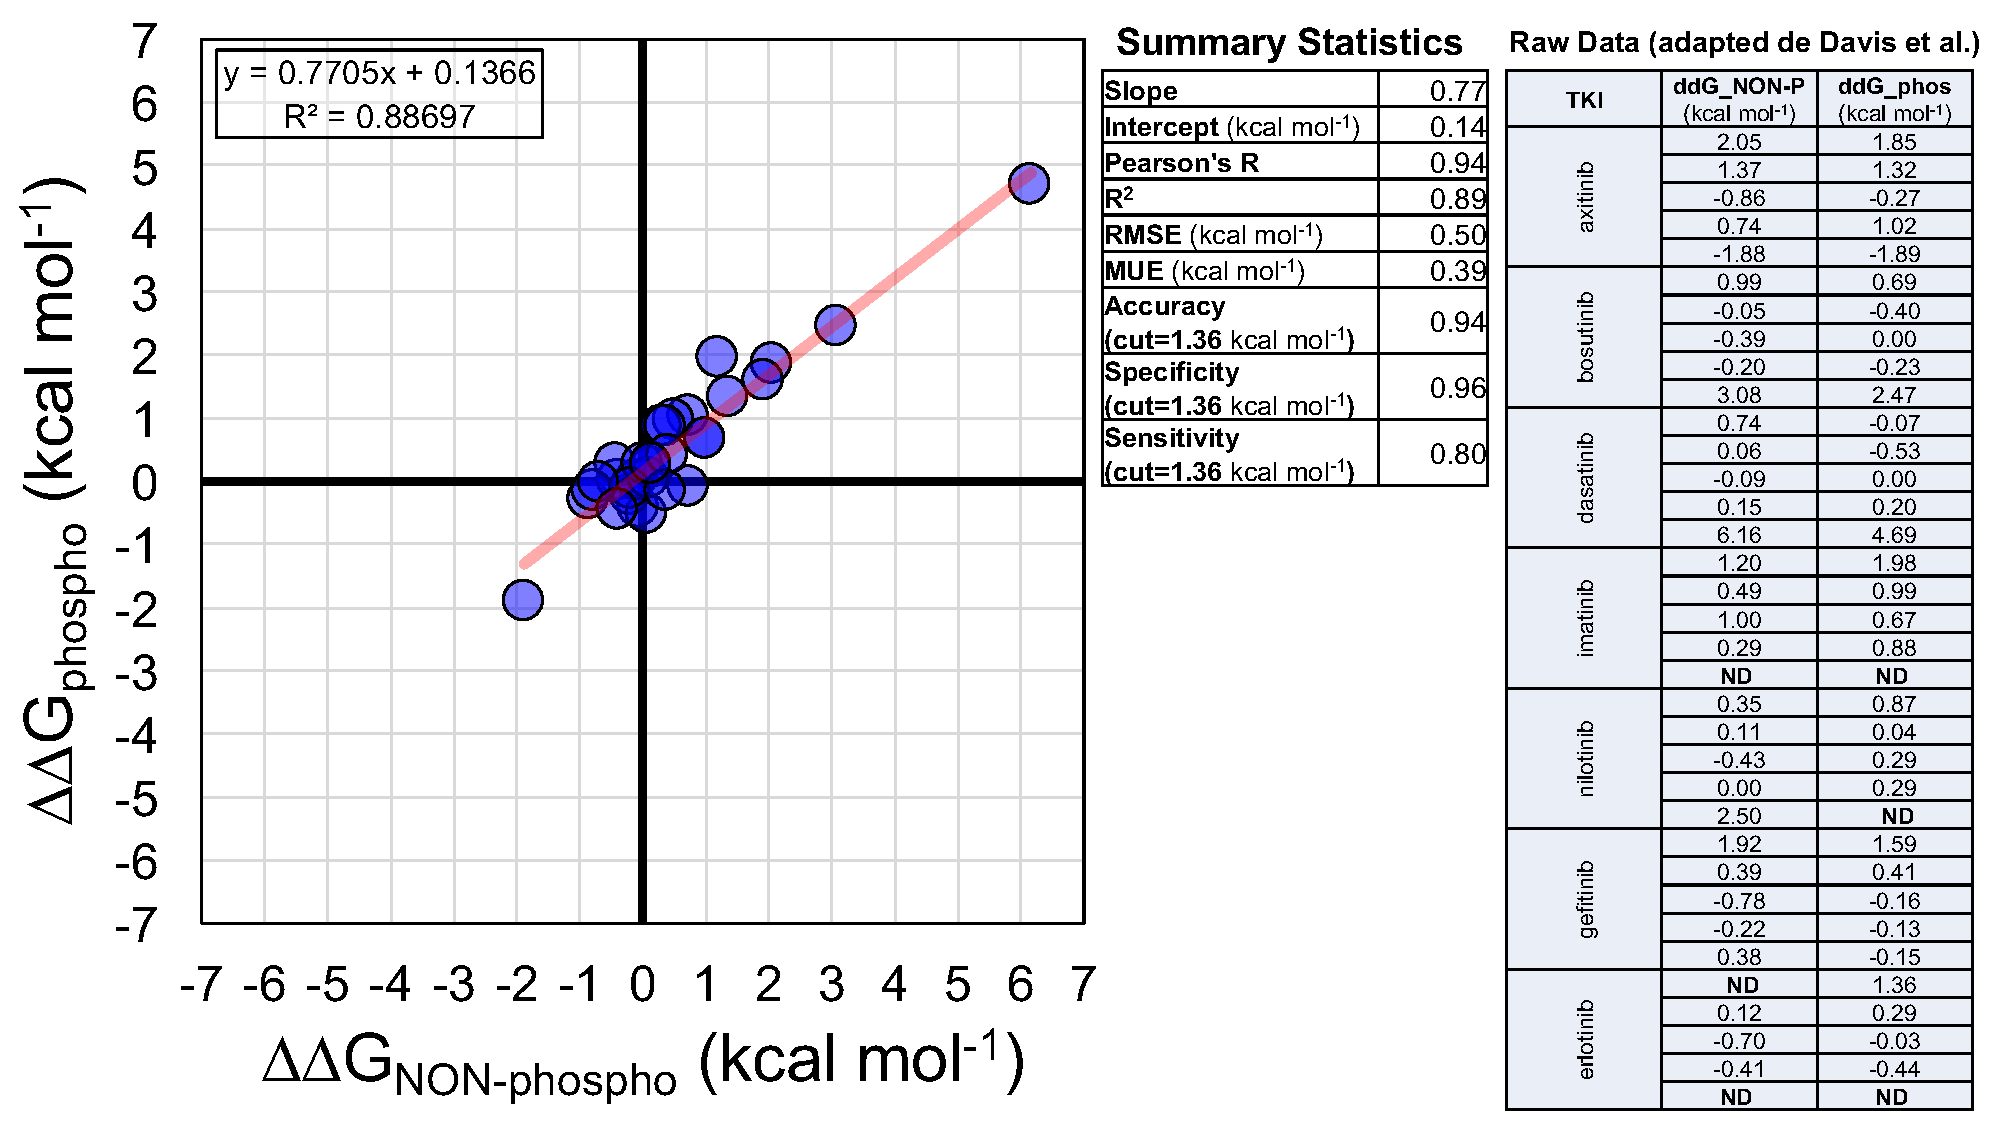
\includegraphics[width=0.8\linewidth]{figures/abl-supplementary-figure-1.pdf}
		\caption[Comparison of 31 mutations for which phosphorylated and non-phosphorylated $\Delta K_{d}$s were available.]{
			{\bf Comparison of 31 mutations for which phosphorylated and non-phosphorylated $\Delta K_{d}$s were available.}
			Scatter plot compares $\Delta\Delta$Gs (derived from the $\Delta K_{d}$s) and contains the best-fit line with slope 0.77 and intercept 0.14. Summary statistics for this comparison are also shown. The raw $\Delta\Delta$Gs used for this comparison were adapted from \protect\cite{Davis:Nat.Biotechnol.:2011}; kino-bead data for ponatinib was not available. \textbf{ND}: No data. \textbf{TKI}: Targeted kinase inhibitor.
		}
		\label{fig:abl-figure-si-1}
	\end{figure}
\end{landscape}

\paragraph{Most mutations do not significantly reduce TKI potency}
The majority of mutations do not lead to resistance by our 10-fold affinity loss threshold: 86.3\% of the co-crystal set (n=113) and 86.8\% of the total set (n=125).
Resistance mutations, which are likely to result in a failure of therapy, constitute 13.7\% of the co-crystal set (n=18) and 13.2\% of the total set of mutations (n=19).
The $\Delta$pIC$_{50}$s for all 144 mutations are summarized in Table \ref{abl-table-si-1}. % in the Supplementary Information.
Two mutations exceeded the dynamic range of the assays (IC$_{50}$ $>$10,000 nM); as these two mutations clearly raise resistance, we excluded them from quantitative analysis (RMSE and MUE) but included them in truth table analyses and classification metrics (accuracy, specificity, sensitivity).

\begin{landscape}
\realsinglespacing
\begin{ThreePartTable}
	\begin{TableNotes}
		\footnotesize
		\item{A}: Gruber et al. (\cite{Gruber:Med.Oncol.:2012}), % \\
		\item{B}: Redaelli et al. (\cite{Redaelli:2012}), % \\
		\item{C}: Cortes et al. (\cite{Cortes:N.Engl.J.Med.:2012}), % \\
		\item{D}: Branford et al. (\cite{Branford:Blood:2002}), % \\
		\item{E}: Press et al. (\cite{Press:2009}), % \\
		\item{F}: Shah et al. (\cite{Shah:CancerCell:2002}), %\\
		\item{G}: F317C observed with $\Delta$27-183, % \\
		\item{H}: M343T observed as compound mutation with H396R, % \\
		\item{I}: L384M observed as compound mutation with M343T, % \\
		\item{J}: H396R observed as compound mutation with F486S, % \\
		\item{K}: F486S observed as compound mutation with H396R 
	\end{TableNotes}
\begin{longtable}[c]{llllllllll}
	\caption[ $\Delta \Delta$G data derived from publicly available $\Delta$pIC$_{50}$ measurements and sources of mutation clinical-observation]{
		{\bf $\Delta \Delta$G data derived from publicly available $\Delta$pIC$_{50}$ measurements and sources of mutation clinical-observation}		
	}
	
 	\label{tab:abl-table-si-1} \\
	\toprule
	{Mutation} 	& {axitinib} 		& {bosutinib}		& {dasatinib}		& {imatinib}		& {nilotinib}		& {ponatinib}		& {gefitinib}		& {erlotinib} 		& {Source of}	\\
	{}			& $\Delta\Delta$G	& $\Delta\Delta$G	& $\Delta\Delta$G	& $\Delta\Delta$G	& $\Delta\Delta$G	& $\Delta\Delta$G	& $\Delta\Delta$G	& $\Delta\Delta$G	& {Clinical}			\\
	{}			& {(kcal/mol)}		& {(kcal/mol)}		& {(kcal/mol)}		& {(kcal/mol)}		& {(kcal/mol)}		& {(kcal/mol)}		& {(kcal/mol)}		& {(kcal/mol)}		&	{Observation}	 \\ \midrule \\
	\endfirsthead
	%
	\multicolumn{10}{c}
	{{\bf Table \thetable\ continued from previous page}} \\
	{Mutation} 	& {axitinib} 		& {bosutinib}		& {dasatinib}		& {imatinib}		& {nilotinib}		& {ponatinib}		& {gefitinib}		& {erlotinib} 		& {Source of}	\\
	{}			& $\Delta\Delta$G	& $\Delta\Delta$G	& $\Delta\Delta$G	& $\Delta\Delta$G	& $\Delta\Delta$G	& $\Delta\Delta$G	& $\Delta\Delta$G	& $\Delta\Delta$G	& {Clinical}			\\
	{}			& {(kcal/mol)}		& {(kcal/mol)}		& {(kcal/mol)}		& {(kcal/mol)}		& {(kcal/mol)}		& {(kcal/mol)}		& {(kcal/mol)}		& {(kcal/mol)}		&{Observation}	\\ \midrule \\
	\endhead

	
		{M244V} & {-0.11}       & {0.43}        & {0.00}        & {0.21}        & {-0.13}       & {0.00}        & {nd}  		& {nd}  	& {A}       \\
		{L248R} & {0.31}        & {1.50}        & {0.65}        & {2.33}        & {2.15}        & {0.58}        & {nd}  		& {nd}  	& {B}     	\\
		{L248V} & {0.32}        & {0.56}        & {0.55}        & {0.64}        & {0.33}        & {0.17}        & {nd}  		& {nd}  	& {A,C}     \\
		{G250E} & {0.27}        & {0.11}        & {0.41}        & {1.01}        & {0.60}        & {0.30}        & {nd}  		& {nd}  	& {A,C,D}   \\
		{Q252H} & {0.20}        & {nd}  		& {nd}  		& {nd}  		& {nd}  		& {nd}  		& {-0.44}       & {-0.13}	& {A}       \\
		{Y253F} & {0.26}        & {-0.34}       & {0.24}        & {1.90}        & {1.48}        & {0.30}        & {-0.17}       & {0.00}	& {C}       \\
		{Y253H} & {0.03}        & {nd} 			& {nd}  		& {nd}  		& {nd}  		& {nd}  		& {nd}  		& {nd}  	& {A,C,D}   \\
		{E255K} & {0.26}        & {0.56}        & {0.90}        & {1.50}        & {1.27}        & {0.41}        & {-0.11}       & {-0.11}	& {A,C,D}   \\
		{E255V} & {0.30}        & {0.66}        & {1.02}        & {2.22}        & {2.36}        & {1.00}        & {nd}  		& {nd}  	& {A,C}     \\
		{D276G} & {0.18}        & {nd}  		& {nd}  		& {nd}  		& {nd}  		& {nd}  		& {nd}  		& {nd}  	& {C}       \\
		{E279K} & {-0.03}       & {nd}  		& {nd}  		& {nd}  		& {nd}  		& {nd}  		& {nd}  		& {nd}  	& {C}       \\
		{E292L} & {0.03}        & {nd}  		& {nd}  		& {nd}  		& {nd}  		& {nd}  		& {nd}  		& {nd}  	& {E}       \\
		{V299L} & {-0.88}       & {1.70}        & {1.24}        & {0.23}        & {0.28}        & {0.17}        & {nd}  		& {nd}  	& {C}       \\
		{T315A} & {-0.45}       & {0.32}        & {2.02}        & {0.51}        & {0.72}        & {0.17}        & {nd}  		& {nd}  	& {C}       \\
		{T315I} & {-1.27}       & {2.45}        & {5.08}        & {2.32}        & {3.75}        & {0.41}        & {nd}  		& {-0.15}   & {C,D}     \\
		{T315V} & {-1.73}       & {nd}  		& {nd}  		& {nd}  		& {nd}  		& {nd}  		& {nd}  		& {nd}  	& {B}     	\\
		{F317C} & {nd}  		& {0.50}        & {1.86}        & {0.28}        & {0.04}        & {0.00}        & {nd}  		& {nd}  	& {A$^{g}$} \\
		{F317I} & {nd}  		& {0.71}        & {1.79}        & {0.17}        & {0.30}        & {0.51}        & {1.35}        & {1.58}    & {C}       \\
		{F317L} & {0.23}        & {0.09}        & {0.96}        & {0.72}        & {0.20}        & {0.17}        & {0.29}        & {0.40}    & {C,D}     \\
		{F317R} & {0.27}        & {nd}  		& {nd}  		& {nd}  		& {nd}  		& {nd}  		& {nd}  		& {nd}  	& {B}		\\
		{F317V} & {0.28}        & {1.72}        & {2.36}        & {0.97}        & {0.33}        & {0.72}        & {nd}  		& {nd}  	& {C}       \\
		{M343T} & {0.21}        & {nd}  		& {nd}  		& {nd}  		& {nd}  		& {nd}  		& {nd}  		& {nd}  	& {F$^{h}$}	\\
		{M351T} & {-0.24}       & {0.19}        & {0.00}        & {0.42}        & {0.00}        & {0.17}        & {0.05}        & {-0.08}	& {A,C,D}	\\
		{E355A} & {nd}  		& {0.02}        & {0.24}        & {0.47}        & {0.11}        & {0.51}        & {nd}  		& {nd}  	& {C}       \\
		{F359C} & {nd}  		& {-0.01}       & {0.00}        & {0.77}        & {0.68}        & {0.41}        & {nd}  		& {nd}  	& {C}       \\
		{F359I} & {0.10}        & {0.04}        & {0.24}        & {0.28}        & {0.86}        & {0.77}        & {nd}  		& {nd}  	& {A}       \\
		{F359V} & {0.07}        & {-0.11}       & {0.00}        & {0.32}        & {0.60}        & {0.17}        & {nd}  		& {nd}  	& {A,C}		\\
		{L384M} & {0.06}        & {nd}  		& {nd}  		& {nd}  		& {nd}  		& {nd}  		& {nd}  		& {nd}  	& {F$^{i}$}	\\
		{H396R} & {0.25}        & {-0.10}       & {0.00}        & {0.40}        & {0.25}        & {0.17}        & {nd}  		& {nd}  	& {A$^{j}$}	\\
		{F486S} & {0.05}        & {nd}  		& {nd}  		& {nd}  		& {nd}  		& {nd}  		& {nd}  		& {nd}  	& {A$^{k}$}	\\
		{E459K} & {nd}  		& {0.35}        & {0.41}        & {0.66}        & {0.55}        & {0.30}        & {nd}  		& {nd}  	& {C}       \\
		\bottomrule
		\insertTableNotes  % tell LaTeX where to insert the contents of "TableNotes"
\end{longtable}
\end{ThreePartTable}
\end{landscape}

\subsection{FEP+ predicts affinity changes for clinical Abl mutants}
Figure~\ref{fig:abl-figure1}B depicts the thermodynamic cycle that illustrates how we used relative free energy calculations to compute the change in ligand binding free energy in response to the introduction of a point mutation in the kinase (Figure~\ref{fig:abl-figure1}C).
From prior experience with relative alchemical free-energy calculations for ligand design, good initial receptor-ligand geometry was critical to obtaining accurate and reliable free energy predictions~\citep{Wang:J.Am.Chem.Soc.:2015}, so we first focused on the 131 mutations in Abl kinase across six TKIs for which wild-type Abl:TKI co-crystal structures were available. Figure~\ref{fig:abl-figure3} summarizes the performance of predicted binding free-energy changes ($\Delta \Delta$G) for all 131 mutants in this set for both a fast MM-GBSA physics-based method that only captures interaction energies for a single structure (Prime) and rigorous alchemical free-energy calculations (FEP+).
Scatter plots compare experimental and predicted free-energy changes ($\Delta\Delta$G) and characterize the ability of these two techniques to predict experimental measurements.
Statistical uncertainty in the predictions and experiment-to-experiment variability in the experimental values are shown as ellipse height and widths respectively.
The value for experimental variability was 0.32 kcal mol$^{-1}$, which was the standard error computed from the cross-comparison in Figure~\ref{fig:abl-figure2}.
For FEP+, the uncertainty was taken to be the standard error of the average from three independent runs for a particular mutation, while Prime results are deterministic and are not contaminated by statistical uncertainty (see Methods).

To better assess whether discrepancies between experimental and computed $\Delta\Delta G$s simply arise for known forcefield limitations or might indicate more significant effects, we incorporated an additional error model in which the forcefield error was taken to be a random error $\sigma_\mathrm{FF} \approx$ 0.9 kcal mol$^{-1}$, a value established form previous benchmarks on small molecules absent conformational sampling or protonation state issues~\cite{Harder:J.Chem.TheoryComput.:2016}.
Thin error bars in Figure~\ref{fig:abl-figure2} represent the overall estimated error due to both this forcefield error and experimental variability or statistical uncertainty. 

To assess overall quantitative accuracy, we computed both root-mean-squared error (RMSE)---which is rather sensitive to outliers, and mean unsigned error (MUE).
For Prime, the MUE was 1.16$^{1.37}_{0.96}$ kcal mol$^{-1}$ and the RMSE was 1.72$^{2.00}_{1.41}$ kcal mol$^{-1}$. 
FEP+, the alchemical free-energy approach, achieved a significantly higher level of quantitative accuracy with an MUE of 0.82$^{0.95}_{0.69}$ kcal mol$^{-1}$ and an RMSE of 1.11$^{1.30}_{0.91}$ kcal mol$^{-1}$.
Notably, alchemical free energy calculations come substantially closer than MMGBSA approach to the minimum achievable RMSE of $0.81^{1.04}_{0.59}$ kcal mol$^{-1}$ (due to experimental error; Figure~\ref{fig:abl-figure2}) for this dataset.


\begin{landscape}
	\begin{figure}[p]
		\centering
		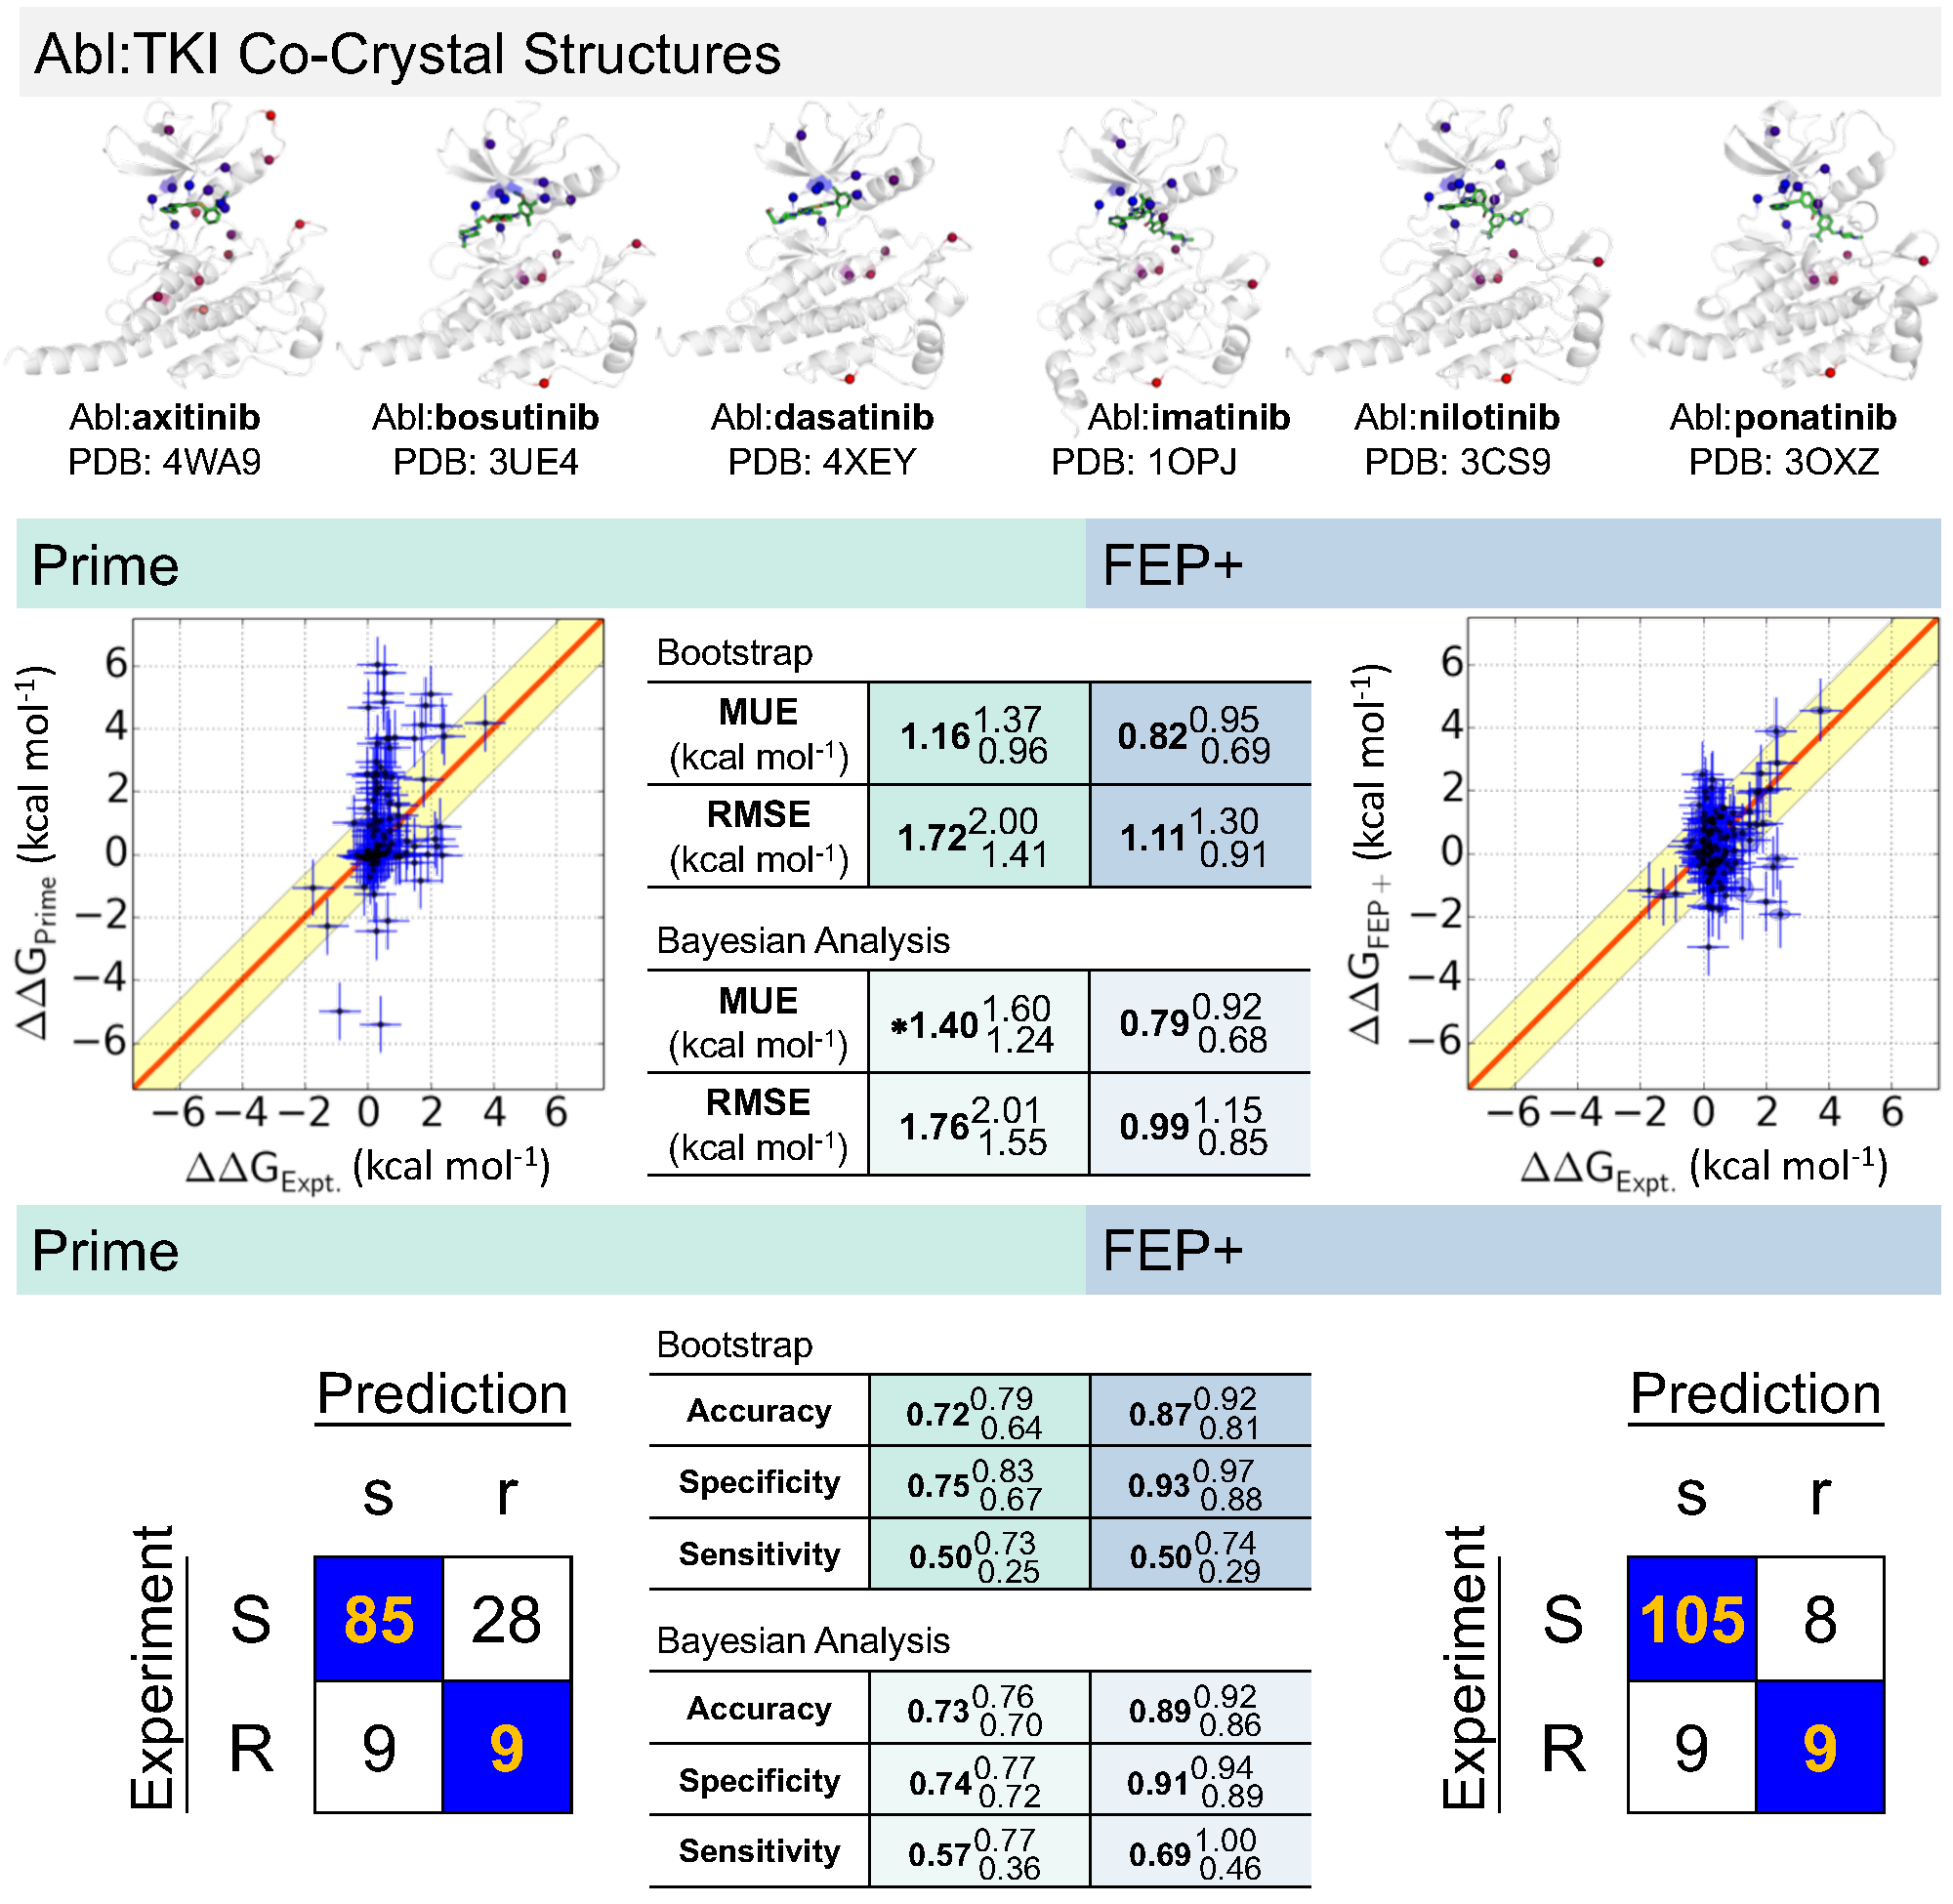
\includegraphics[width=0.7\linewidth]{figures/abl-figure-3.pdf}
		\caption[Comparison of experimentally-measured binding free-energy changes ($\Delta \Delta$G) for 131 clinically observed mutations and 6 selective kinase inhibitors for which co-crystal structures of wild-type kinase with inhibitor are available.]{
		Continued on the next page 
	}
		\label{fig:abl-figure3}
	\end{figure}
\end{landscape}
\addtocounter{figure}{-1}
\begin{landscape}
	\begin{figure}
		\caption[Figure caption]{{\bf Comparison of experimentally-measured binding free-energy changes ($\Delta \Delta$G) for 131 clinically observed mutations and 6 selective kinase inhibitors for which co-crystal structures of wild-type kinase with inhibitor are available.}
			\emph{Top panel:} Abl:TKI co-crystal structures used in this study with locations of clinical mutants for each inhibitor highlighted (colored from blue to red for residues nearest to farthest from ligand) in relation to TKI (green sticks) on the corresponding Abl:TKI wild-type crystal structure.
			\emph{Middle panel:} Scatter plots show Prime and FEP+ computed $\Delta \Delta $G compared to experiment, with ellipse widths and heights ($\pm\sigma$) for experiment and FEP+ respectively.
			The red diagonal line indicates when prediction equals experiment, while the yellow shaded region indicates area in which predicted $\Delta \Delta$G is within 1.36 kcal mol$^{-1}$ of experiment (corresponding to a ten-fold error in predicted affinity change).
			$\Delta \Delta$G < 0 kcal mol$^{-1}$ denotes the mutation increases the susceptibility of the kinase to the inhibitor, while $\Delta \Delta$G > 0 kcal mol$^{-1}$ denotes the mutation increases the resistance of the kinase to the inhibitor.
			The two mutations that were beyond the concentration limit of the assay (T315I/dasatinib, L248R/imatinib) were not plotted; 129 points were plotted.
			Truth tables of classification accuracy, sensitivity and specificity using two-classes. 
			\emph{Bottom panel:} Truth tables and classification results include T315I/dasatinib and L248R/imatinib; 131 points were used.
			For MUE, RMSE, and truth table performance statistics, sub/superscripts denote 95 \% CIs. 
			Variability in the experimental data is shown as ellipse widths and uncertainty in our calculations is shown as ellipse heights. 
			Experimental variability was computed as the standard error between IC$_{50}$-derived $\Delta \Delta G$ measurements made by different labs, 0.32 kcal mol$^{-1}$. 
			The statistical uncertainty in the Prime calculations was zero because the method is deterministic ($\sigma_\mathrm{cal}=0$), while the uncertainty in the FEP+ calculations was reported as the standard error, $\sigma_\mathrm{cal}$, of the mean of the predicted $\Delta \Delta G$s from three independent runs. 
			To better highlight true outliers unlikely to simply result from expected forcefield error, we presume forcefield error ($\sigma_\mathrm{FF} \approx$ 0.9 kcal mol$^{-1}$~\cite{Harder:J.Chem.TheoryComput.:2016}) also behaves as a random error, and represent the total estimated statistical and forcefield error ($\sqrt{\sigma_\mathrm{FF}^2 + \sigma_\mathrm{exp/cal}^2}$) as vertical error bars. 
			The horizontal error bars for the experiment ($\sigma_\mathrm{exp}$) was computed as the standard error between $\Delta$pIC$_{50}$ and $\Delta$K$_{d}$ measurements, 0.58 kcal mol$^{-1}$.
			For Prime, \textbf{*MUE} highlights that the Bayesian model yields a value for MUE that is noticeably larger than MUE for observed data due to the non-Gaussian error distribution of Prime.}
	\end{figure}
\end{landscape}

\subsection{FEP+ accurately classifies affinity changes for Abl mutants}
While quantitative accuracy (MUE, RMSE) is a principle metric of model performance, an application of potential interest is the ability to classify mutations as causing resistance to a specific TKI.
To characterize the accuracy with which Prime and FEP+ classified mutations in a manner that might be therapeutically relevant, we classified mutations by their experimental impact on the binding affinity as susceptible (affinity for mutant is diminished by no more than 10-fold, $\Delta \Delta G \leq$ 1.36 kcal mol$^{-1}$) or as resistant (affinity for mutant is diminished by least 10-fold, $\Delta \Delta G >$ 1.36 kcal mol$^{-1}$).    
Summary statistics of experimental and computational predictions of these classes are shown in Figure~\ref{fig:abl-figure2} (bottom) as truth tables (also known as confusion matrices).

The simple minimum-energy scoring method Prime correctly classified 9 of the 18 resistance mutations in the dataset while merely 85 of the 113 susceptible mutations were correctly classified (28 false positives).
In comparison, the alchemical free-energy method FEP+, which includes entropic and enthalpic contributions as well as explicit representation of solvent, correctly classified 9 of the 18 resistance mutations while a vast majority, 105, of the susceptible mutations were correctly classified (merely 8 false positives).
Prime achieved a classification accuracy of 0.72$^{0.79}_{0.64}$, while FEP+ achieved an accuracy that is significantly higher (both in a statistical sense and in overall magnitude), achieving an accuracy of 0.87$^{0.92}_{0.81}$.
Sensitivity (also called true positive rate) and specificity (true negative rate) are also informative statistics in assessing the performance of a binary classification scheme.
For Prime, the sensitivity was 0.50$^{0.73}_{0.25}$, while the specificity was 0.75$^{0.83}_{0.67}$.
To put this in perspective, a CML patient bearing a resistance mutation in the kinase domain of Abl has an equal chance of Prime correctly predicting this mutation would be resistant to one of the TKIs considered here, while if the mutation was susceptible, the chance of correct prediction would be $\sim$75\%.
By contrast, the classification specificity of FEP+ was substantially better.
For FEP+, the sensitivity was 0.50$^{0.74}_{0.29}$ while the specificity was 0.93$^{0.97}_{0.88}$.
There is a very high probability that FEP+ will correctly predict that one of the eight TKIs studied here will remain effective for a patient bearing a susceptible mutation. 

\subsection{How reliant are classification results on choice of cutoff?}
Previous work by O'Hare et al. utilized TKI-specific thresholds for dasatinib, imatinib, and nilotinib~\citep{OHare:Clin.CancerRes.:2005}, which were $\sim$2 kcal mol$^{-1}$. Figure \ref{fig:figure-si-2} shows that when our classification threshold was increased to a 20-fold change in binding (1.77 kcal mol$^{-1}$), FEP+ correctly classified 8 of the 13 resistant mutations and with a threshold of 100-fold change in binding (2.72 kcal mol$^{-1}$), FEP+ correctly classified the only two resistant mutations (T315I/dasatinib and T315I/nilotinib).
With the extant multilayered and multinodal decision-making algorithms used by experienced oncologists to manage their patients' treatment, or by medicinal chemists to propose candidate compounds for clinical trials, the resistant or susceptible cutoffs could be selected with more nuance than the simple 10-fold affinity threshold we consider here.
With a larger affinity change cutoff, for example, the accuracy with which physical models predict resistance mutations increases beyond 90\% (Figure \ref{fig:figure-si-2}).
For the alchemical approach, the two-class accuracy was $0.92^{0.96}_{0.87}$ when an affinity change cutoff of 20-fold was used while using an affinity change cutoff of 100-fold further improved the two-class accuracy to $0.98^{1.00}_{0.96}$.

\begin{landscape}
	\begin{figure}[p]
		\centering
		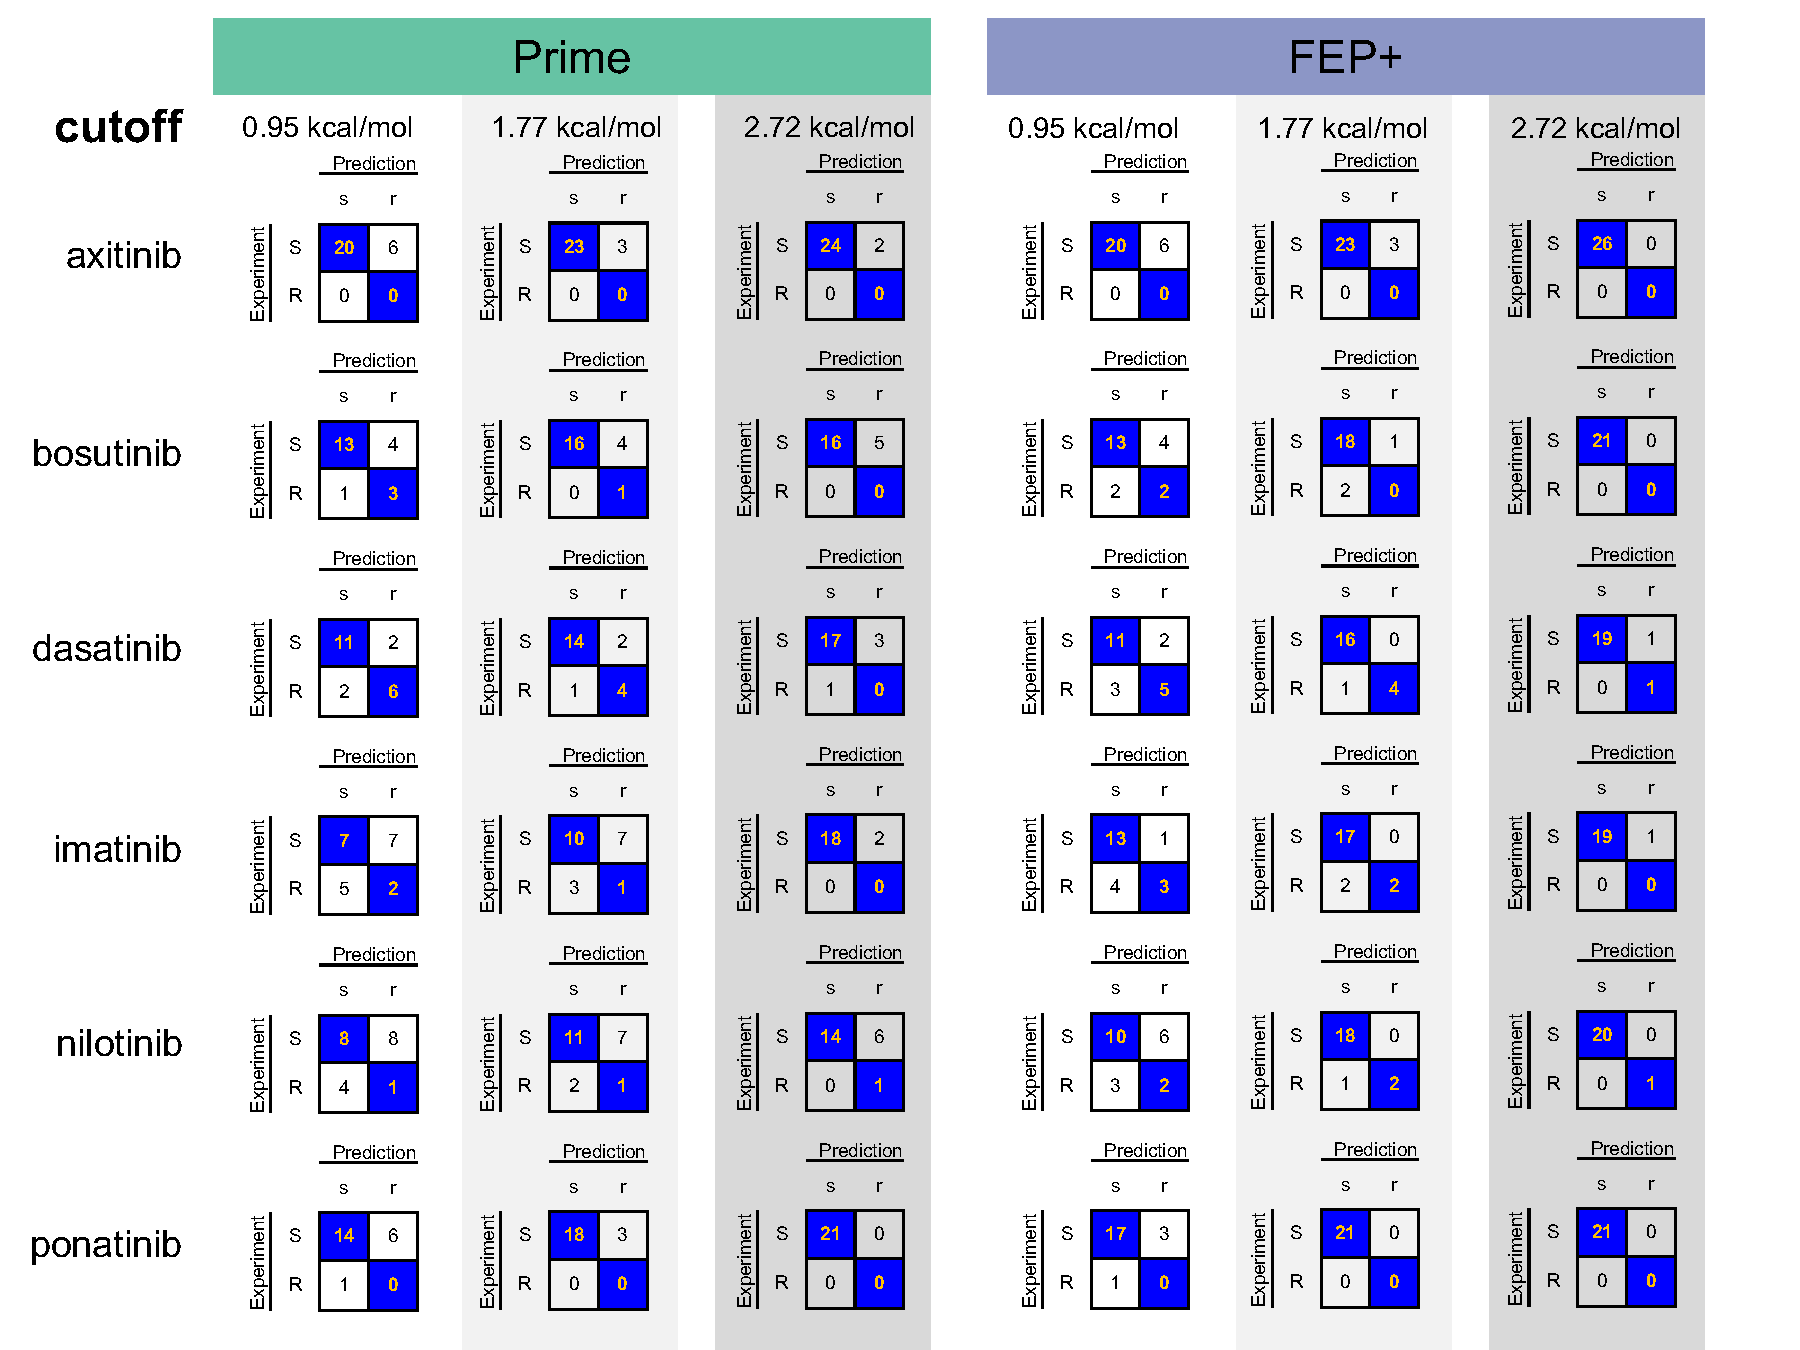
\includegraphics[width=0.8\linewidth]{figures/abl-supplementary-figure-2.pdf}
		\caption[TKI-by-TKI truth tables with increasingly large classification cutoffs.]{
			{\bf TKI-by-TKI truth tables with increasingly large classification cutoffs.}
			Truth tables for the six TKIs (axitinib, bosutinib, dasatinib, imatinib, nilotinib, and ponatinib) using Prime (left, green) and FEP+ (right, blue) with classification cutoff values defining whether mutations are susceptible (S, experiment; s, prediction) or resistant (R, experiment; r, prediction). 
			A mutation is susceptible if $\Delta\Delta$G $\le$ \textbf{cutoff} or resistant if $\Delta\Delta$G > \textbf{cutoff}.
		}
		\label{fig:abl-figure-si-2}
	\end{figure}
\end{landscape}

\subsection{Bayesian analysis can estimate the true error}
The statistical metrics---MUE, RMSE, accuracy, specificity, and sensitivity---discussed above are based on analysis of the apparent performance of the observed modeling results compared with the observed experimental data via sample statistics.
However, this analysis considers a limited number of mutants, and both measurements and computed values are contaminated with experimental or statistical error. 
To obtain an estimate of the \emph{intrinsic performance} of our physical modeling approaches, accounting for known properties of the experimental variability and statistical uncertainties, we used a hierarchical Bayesian model (detailed in the Methods) to infer posterior predictive distributions from which expectations and 95\% predictive intervals could be obtained.
The results of this analysis are presented in Figure~\ref{fig:abl-figure3} (central tables). 

FEP+ is significantly better than Prime at predicting the impact of mutations on TKI binding affinities, as the apparent performance (using the original observations) as well as the intrinsic performance (where Bayesian analysis was used to correct for statistical uncertainty or experimental variation) were well-separated outside their 95\% confidence intervals in nearly all metrics.
Applying the Bayesian model, the MUE and RMSE for FEP+ was $0.79^{0.92}_{0.68}$ kcal mol$^{-1}$ and $0.99^{1.15}_{0.85}$ kcal mol$^{-1}$ respectively (N=129). 
For the classification metrics accuracy, specificity, and sensitivity, the model yields $0.89^{0.92}_{0.86}$, $0.91^{0.94}_{0.89}$, and $0.69^{1.00}_{0.46}$ respectively (N=131).
The intrinsic RMSE and MUE of Prime was $1.76^{2.01}_{1.55}$ kcal mol$^{-1}$ and $1.40^{1.60}_{1.24}$ kcal mol$^{-1}$ (N=129) respectively, and the classification accuracy, specificity, and sensitivity was $0.73^{0.76}_{0.70}$, $0.74^{0.77}_{0.72}$, and $0.57^{0.77}_{0.36}$ respectively (N=131).
The intrinsic MUE of Prime obtained by this analysis is larger than the observed MUE reflecting the non-Gaussian, fat-tailed error distributions of Prime results.


\subsection{How transferable is FEP+ across the six TKIs?}
The impact of point mutations on drug binding are not equally well predicted for the six TKIs.
Figure~\ref{fig:abl-figure4} expands the results in Figure~\ref{fig:abl-figure3} on a TKI-by-TKI basis to dissect the particular mutations in the presence of a specific TKI.
%axitinib
Prime and FEP+ correctly predicted that most mutations in this dataset (N=26) do not raise resistance to axitinib, though FEP+ predicted 4 false positives compared with 3 false positives by Prime. The MUE and RMSE of FEP+ was excellent for this inhibitor, $0.70^{0.93}_{0.50}$ kcal mol$^{-1}$ and $0.91^{1.14}_{0.64}$ kcal mol$^{-1}$ respectively.
%bosutinib
While the classification results for bosutinib (N=21) were equally well predicted by Prime as by FEP+, FEP+ was still able to achieve superior, but not highly significant, predictive performance for the quantitative metrics MUE and RMSE, which were $0.96^{1.42}_{0.55}$ kcal mol$^{-1}$ and $1.41^{1.97}_{0.77}$ kcal mol$^{-1}$ respectively (FEP+) and $1.13^{1.83}_{0.60}$ kcal mol$^{-1}$ and $1.80^{2.62}_{0.92}$ kcal mol$^{-1}$ respectively (Prime).
%dasatinib
For dasatinib, FEP+ achieved an MUE and RMSE of $0.76^{1.13}_{0.49}$ kcal mol$^{-1}$ and $1.07^{1.57}_{0.59}$ kcal mol$^{-1}$ respectively whereas the results were, as expected, less quantitatively predictive for Prime (N=20).
%imatinib
The results for imatinib were similar to those of dasatinib above, where the MUE and RMSE for FEP+ were $0.82^{1.15}_{0.53}$ kcal mol$^{-1}$ and $1.09^{1.43}_{0.69}$ kcal mol$^{-1}$ respectively (N=20).
%nilotinib
Nilotinib, a derivative of imatinib, led to nearly identical quantitative performance results for FEP+ with an MUE and RMSE of $0.82^{1.12}_{0.57}$ kcal mol$^{-1}$ and $1.06^{1.39}_{0.69}$ kcal mol$^{-1}$ respectively (N=21).
%ponatinib
Similar to axitinib, ponatinib presented an interesting case because there were no mutations in this dataset that raised resistance to it.
Despite the wide dynamic range in the computed values of $\Delta\Delta$G for other inhibitors, FEP+ correctly predicted a very narrow range of $\Delta\Delta$Gs for this drug. 
This is reflected in the MUE and RMSE of $0.87^{1.16}_{0.62}$ kcal mol$^{-1}$ and $1.09^{1.46}_{0.70}$ kcal mol$^{-1}$ respectively, which are in-line with the MUEs and RMSEs for the other TKIs.

\begin{landscape}
	\begin{figure}[p]
		\centering
		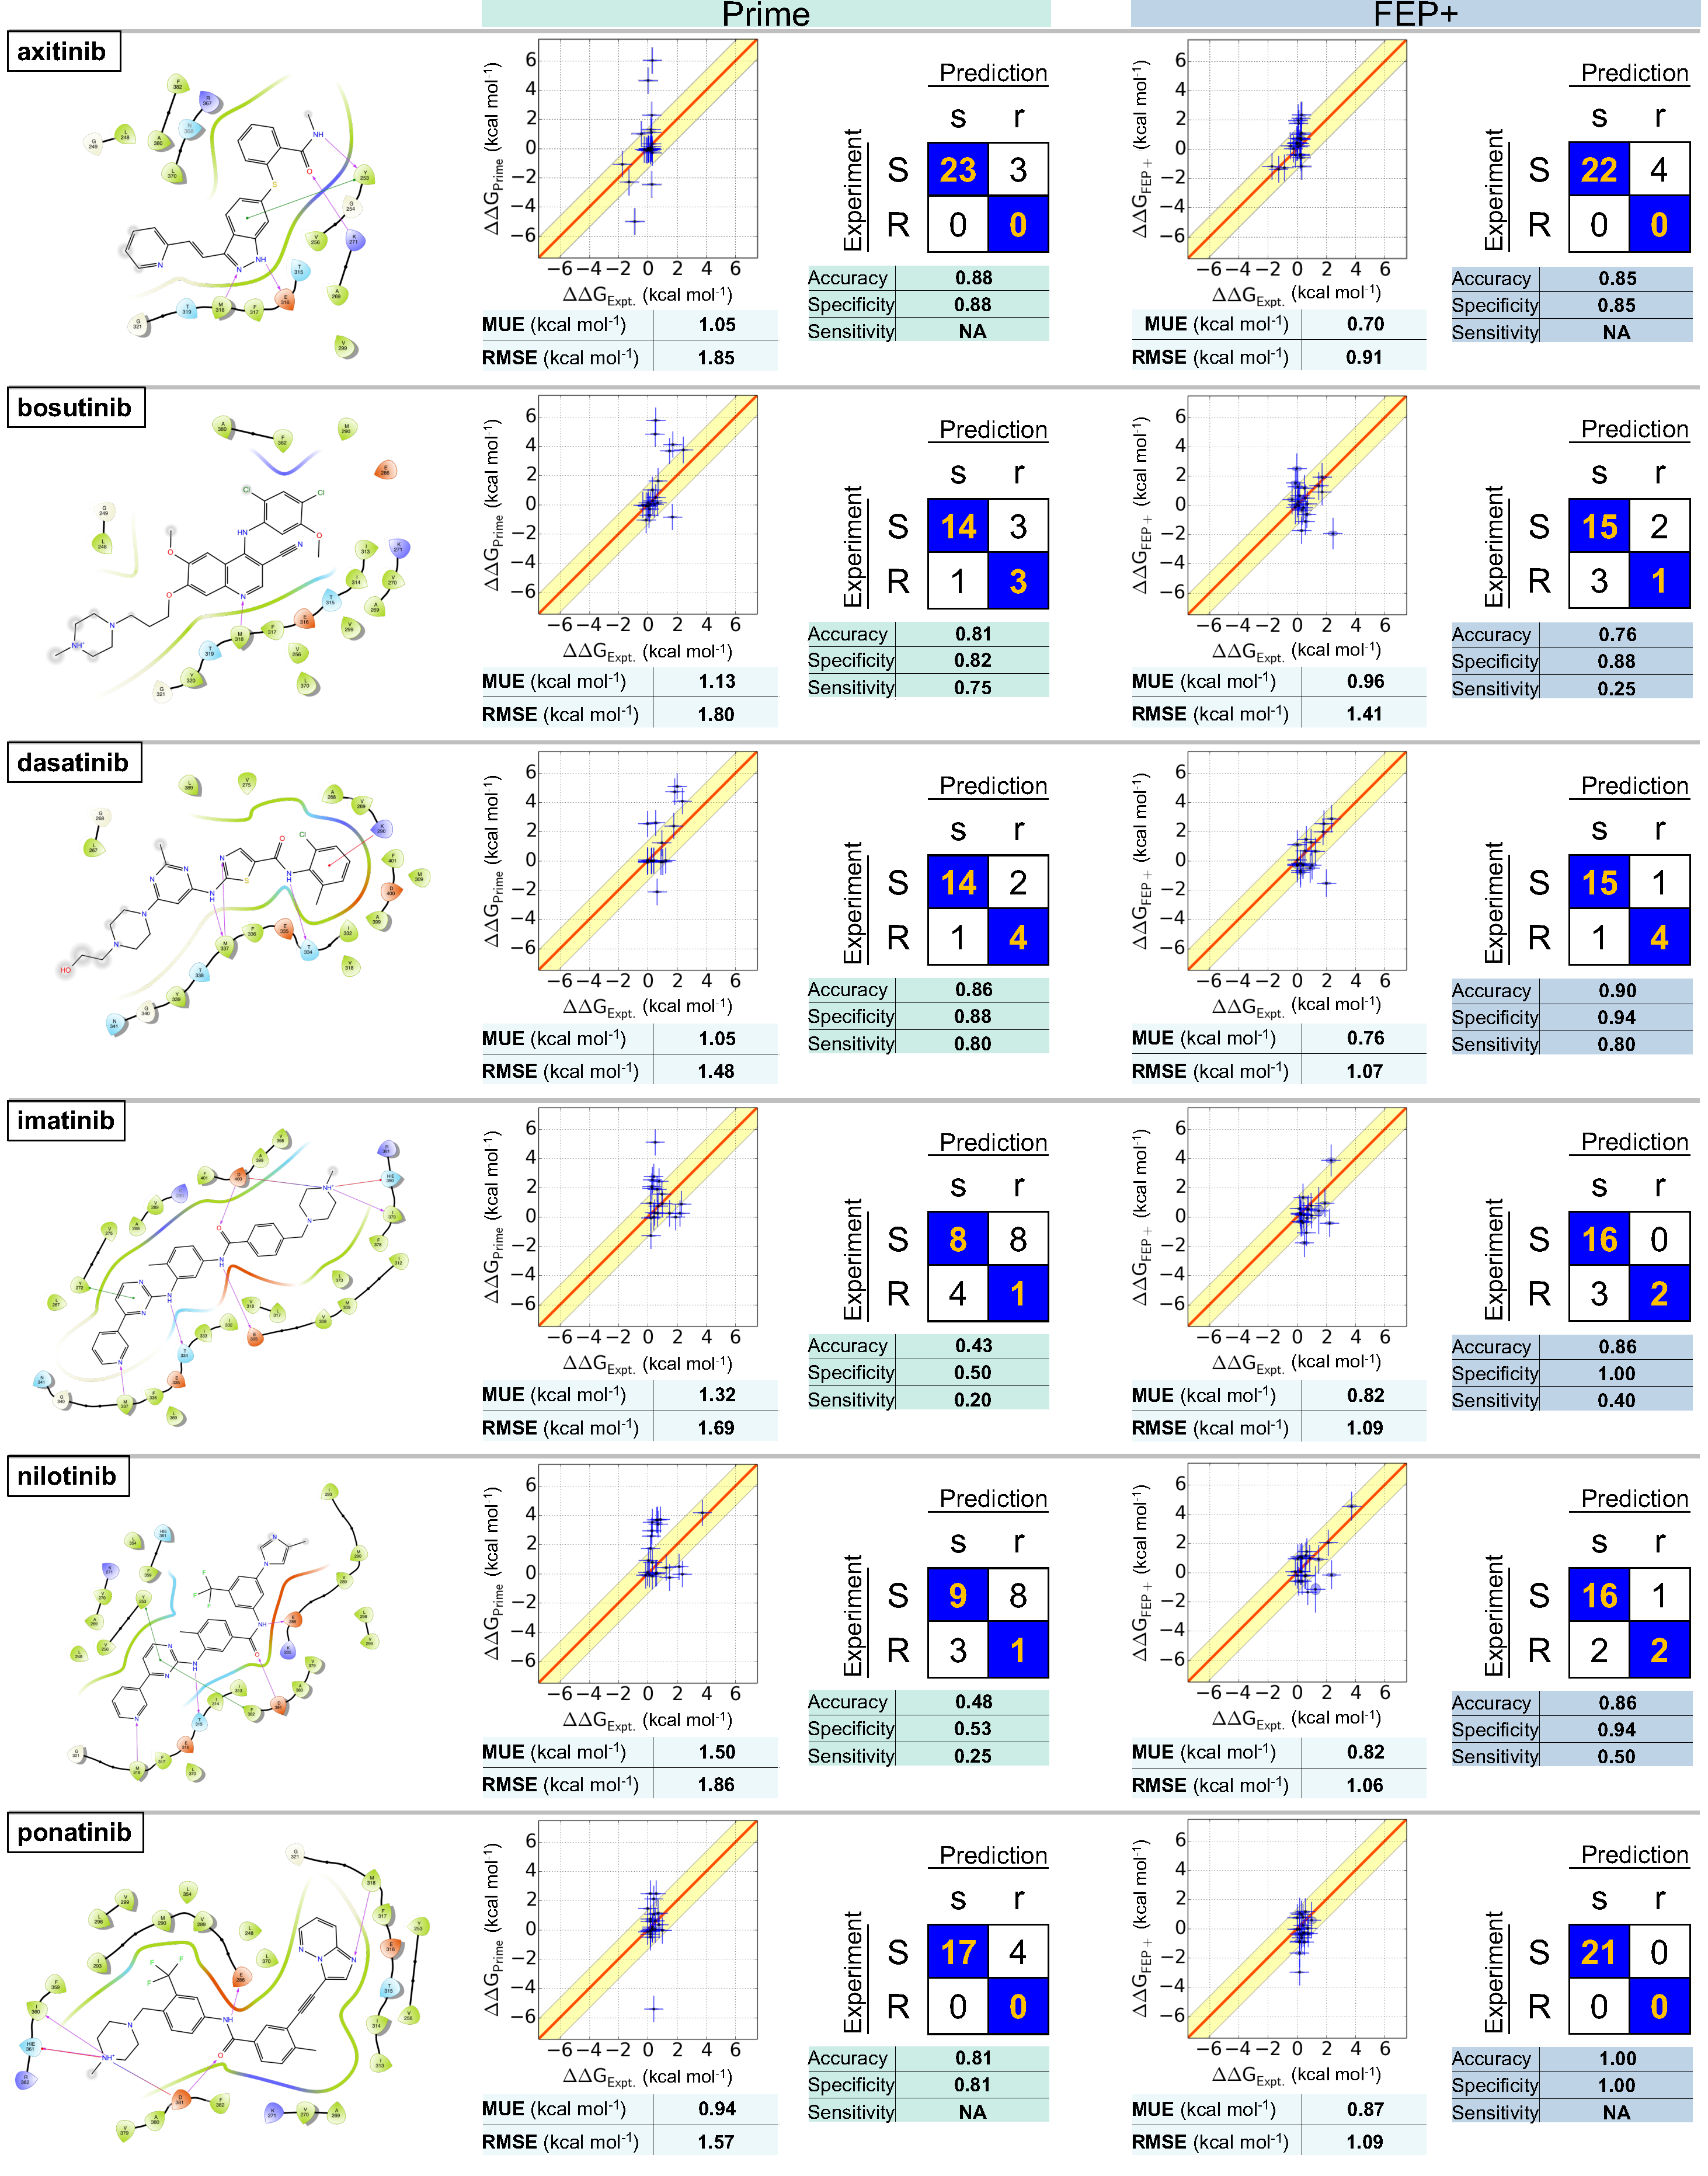
\includegraphics[width=0.5\linewidth]{figures/abl-figure-4.pdf}
		\caption[Physical modeling accuracy in computing the impact of clinical Abl mutations on selective inhibitor binding.]{
			Continued on the next page
			}
		\label{fig:abl-figure4}
	\end{figure}
\end{landscape}
\addtocounter{figure}{-1}
\begin{landscape}
	\begin{figure}
		\caption[Figure caption]{{\bf Physical modeling accuracy in computing the impact of clinical Abl mutations on selective inhibitor binding.}
			Ligand interaction diagrams for six selective FDA-approved tyrosine kinase inhibitors (TKIs) for which co-crystal structures with Abl were available (left). Comparisons for clinically-observed mutations are shown for FEP+ (right) and Prime (left).
			For each ligand, computed \emph{vs.} experimental binding free energies ($\Delta \Delta$G) are plotted with MUE and RMSE (units of kcal mol$^{-1}$) depicted below.
			Truth tables are shown to the right.
			Rows denote \emph{true} susceptible (S, $\Delta \Delta$G $\leq$ 1.36 kcal mol$^{-1}$) or resistant (R, $\Delta \Delta$G > kcal mol$^{-1}$) experimental classes using a 1.36 kcal mol$^{-1}$ (10-fold change) threshold;
			columns denote \emph{predicted} susceptible (s, $\Delta \Delta$G $\leq$ kcal mol$^{-1}$) or resistant (r, $\Delta \Delta$G > kcal mol$^{-1}$).
			Correct predictions populate diagonal elements (orange text), incorrect predictions populate off-diagonals.
			Accuracy, specificity, and sensitivity for two-class classification are shown below the truth table.
			Elliptical point sizes and error bars in the scatter plots depict estimated uncertainty/variability and error respectively ($\pm\sigma$) of FEP+ values (vertical size) and experimental values (horizontal size).
			Note: The sensitivity for axitinib and ponatinib is NA, because there is no resistant mutation for these two drugs.
		}
	\end{figure}
\end{landscape}


\subsection{Understanding the origin of mispredictions}
Resistance mutations that are mispredicted as susceptible (false negatives) are particularly critical because they might mislead the clinician or drug designer into believing the inhibitor will remain effective against the target.
Which resistance mutations did FEP+ mispredict as susceptible?
Nine mutations were classified by FEP+ to be susceptible when experimentally measured $\Delta$pIC$_{50}$ data indicate the mutations should have increased resistance according to our 10-fold affinity cutoff for resistance.
Notably, the 95\% confidence intervals for five of these mutations spanned the 1.36 kcal mol$^{-1}$ threshold, indicating these misclassifications are not statistical significant when the experimental error and statistical uncertainty in FEP+ are accounted for:
bosutinib/L248R ($\Delta\Delta$G$_{FEP+}$=$1.32^{1.94}_{0.70}$ kcal mol$^{-1}$), 
imatinib/E255K ($\Delta\Delta$G$_{FEP+}$=$0.43^{3.05}_{-2.19}$ kcal mol$^{-1}$), 
imatinib/Y253F ($\Delta\Delta$G$_{FEP+}$=$0.95^{1.64}_{0.26}$ kcal mol$^{-1}$), 
and nilotinib/Y253F ($\Delta\Delta$G$_{FEP+}$=$0.89^{1.69}_{0.09}$ kcal mol$^{-1}$). 
The bosutinib/V299L mutation was also not significant because the experimental $\Delta\Delta$G, $1.70^{2.33}_{1.08}$ kcal mol$^{-1}$, included the 1.36 kcal mol$^{-1}$ cutoff; the value of $\Delta\Delta$G predicted by FEP+ for this mutation was $0.91^{1.02}_{0.79}$ kcal mol$^{-1}$, the upper bound of the predicted value was within 0.06 kcal mol$^{-1}$ of the lower bound of the experimental value.

Four mutations, however, were misclassified to a degree that is statistically significant given their 95\% confidence intervals:
dasatinib/T315A, bosutinib/T315I, imatinib/E255V, and nilotinib/E255V.
For dasatinib/T315A, although the T315A mutations for bosutinib, imatinib, nilotinib, and ponatinib were correctly classified as susceptible, the predicted free energy changes for these four TKIs were consistently much more negative than the corresponding experimental measurements, just as for dasatinib/T315A, indicating there might be a generic driving force contributing to the errors in T315A mutations for these five TKIs. 
Abl is known to be able to adopt many different conformations (including DFG-in and DFG-out), and it is very likely that the T315A mutation will induce conformational changes in the apo protein~\citep{Shan:Proc.Natl.Acad.Sci.:2009}, which was not adequately sampled in the relatively short simulations, leading to the errors for T315A mutations for these TKIs.    
By comparison, the T315I mutations for axitinib, bosutinib, imatinib, nilotinib, and ponatinib were all accurately predicted with the exception of bosutinib/T315I being the only misprediction, suggesting an issue specific to bosutinib.
The complex electrostatic interactions between the 2,4-dichloro-5-methoxyphenyl ring in bosutinib and the adjacent positively charged amine of the catalytic Lys271 may not be accurately captured by the fixed-charge OPLS3 force field, leading to the misprediction for bosutinib/T315I mutation.

Insufficient sampling might also belie the imatinib/E255V and nilotinib/E255V mispredictions because they reside in the highly flexible P-loop.
Since E255V was a charge change mutation, we utilized a workflow that included a transmutable explicit ion (see Methods).
The distribution of these ions in the simulation box around the solute might not have converged to their equilibrium state on the relatively short timescale of our simulations (5 ns), and the insufficient sampling of ion distributions coupled with P-loop motions might lead to misprediction of these two mutations.

\subsection{How strongly is accuracy affected for docked TKIs?}
To assess the potential for utilizing physics-based approaches in the absence of a high-resolution experimental structure, we generated models of Abl bound to two TKIs---erlotinib and gefinitib---for which co-crystal structures with wild-type kinase are not currently available.
In Figure~\ref{fig:abl-figure5}, we show the Abl:erlotinib and Abl:gefitinib complexes that were generated using a docking approach (Glide-SP, see Methods). 
These two structures were aligned against the co-crystal structures of EGFR:erlotinib and EGFR:gefinitib to highlight the structural similarities between the binding pockets of Abl and EGFR and the TKI binding mode in Abl versus EGFR.
As an additional test of the sensitivity of FEP+ to system preparation, a second set of Abl:erlotinib and Abl:gefitinib complexes was generated in which crystallographic water coordinates were transferred to the docked inhibitor structures (see Methods).

Alchemical free-energy simulations were performed on 13 mutations between the two complexes; 7 mutations for erlotinib and 6 mutations for gefitinib.
The quantitative accuracy of FEP+ in predicting the value of $\Delta \Delta$G was excellent---MUE and RMSE of $0.58^{0.86}_{0.33}$ kcal mol$^{-1}$ and $0.80^{1.09}_{0.44}$ kcal mol$^{-1}$ respectively if crystal waters are omitted, and $0.50^{0.78}_{0.26}$ kcal mol$^{-1}$ and $0.69^{0.97}_{0.35}$ kcal mol$^{-1}$ if crystal waters were restored after docking.
Encouragingly, these results indicate that our initial models of Abl bound to erlotinib and gefitinib were reliable because the accuracy and dependability of our FEP+ calculations were not sensitive to crystallographic waters.
Our secondary concern was the accuracy with which the approach classified mutations as resistant or susceptible.

 While the results presented in (Figure~\ref{fig:abl-figure5}) indicate that FEP+ is capable of achieving good quantitative accuracy when a co-crystal structure is unavailable, it is important to understand why a mutation was predicted to be susceptible but was determined experimentally to be resistant.
F317I was the one mutation that increased resistance to erlotinib (or gefitinib) because it destabilized binding by more than 1.36 kcal mol$^{-1}$---$1.35^{1.67}_{1.03}$ kcal mol$^{-1}$ (gefitinib) and $1.58^{1.90}_{1.26}$ kcal mol$^{-1}$ (erlotinib), but the magnitude of the experimental uncertainty means we are unable to confidently discern whether this mutation induces more than 10-fold resistance to either TKI.
Therefore, the one misclassification by FEP+ in Figure~\ref{fig:abl-figure5} is not statistically significant and the classification metrics presented there underestimate the nominal performance of this alchemical free-energy method.

\begin{landscape}
	\begin{figure}[p]
		\centering
		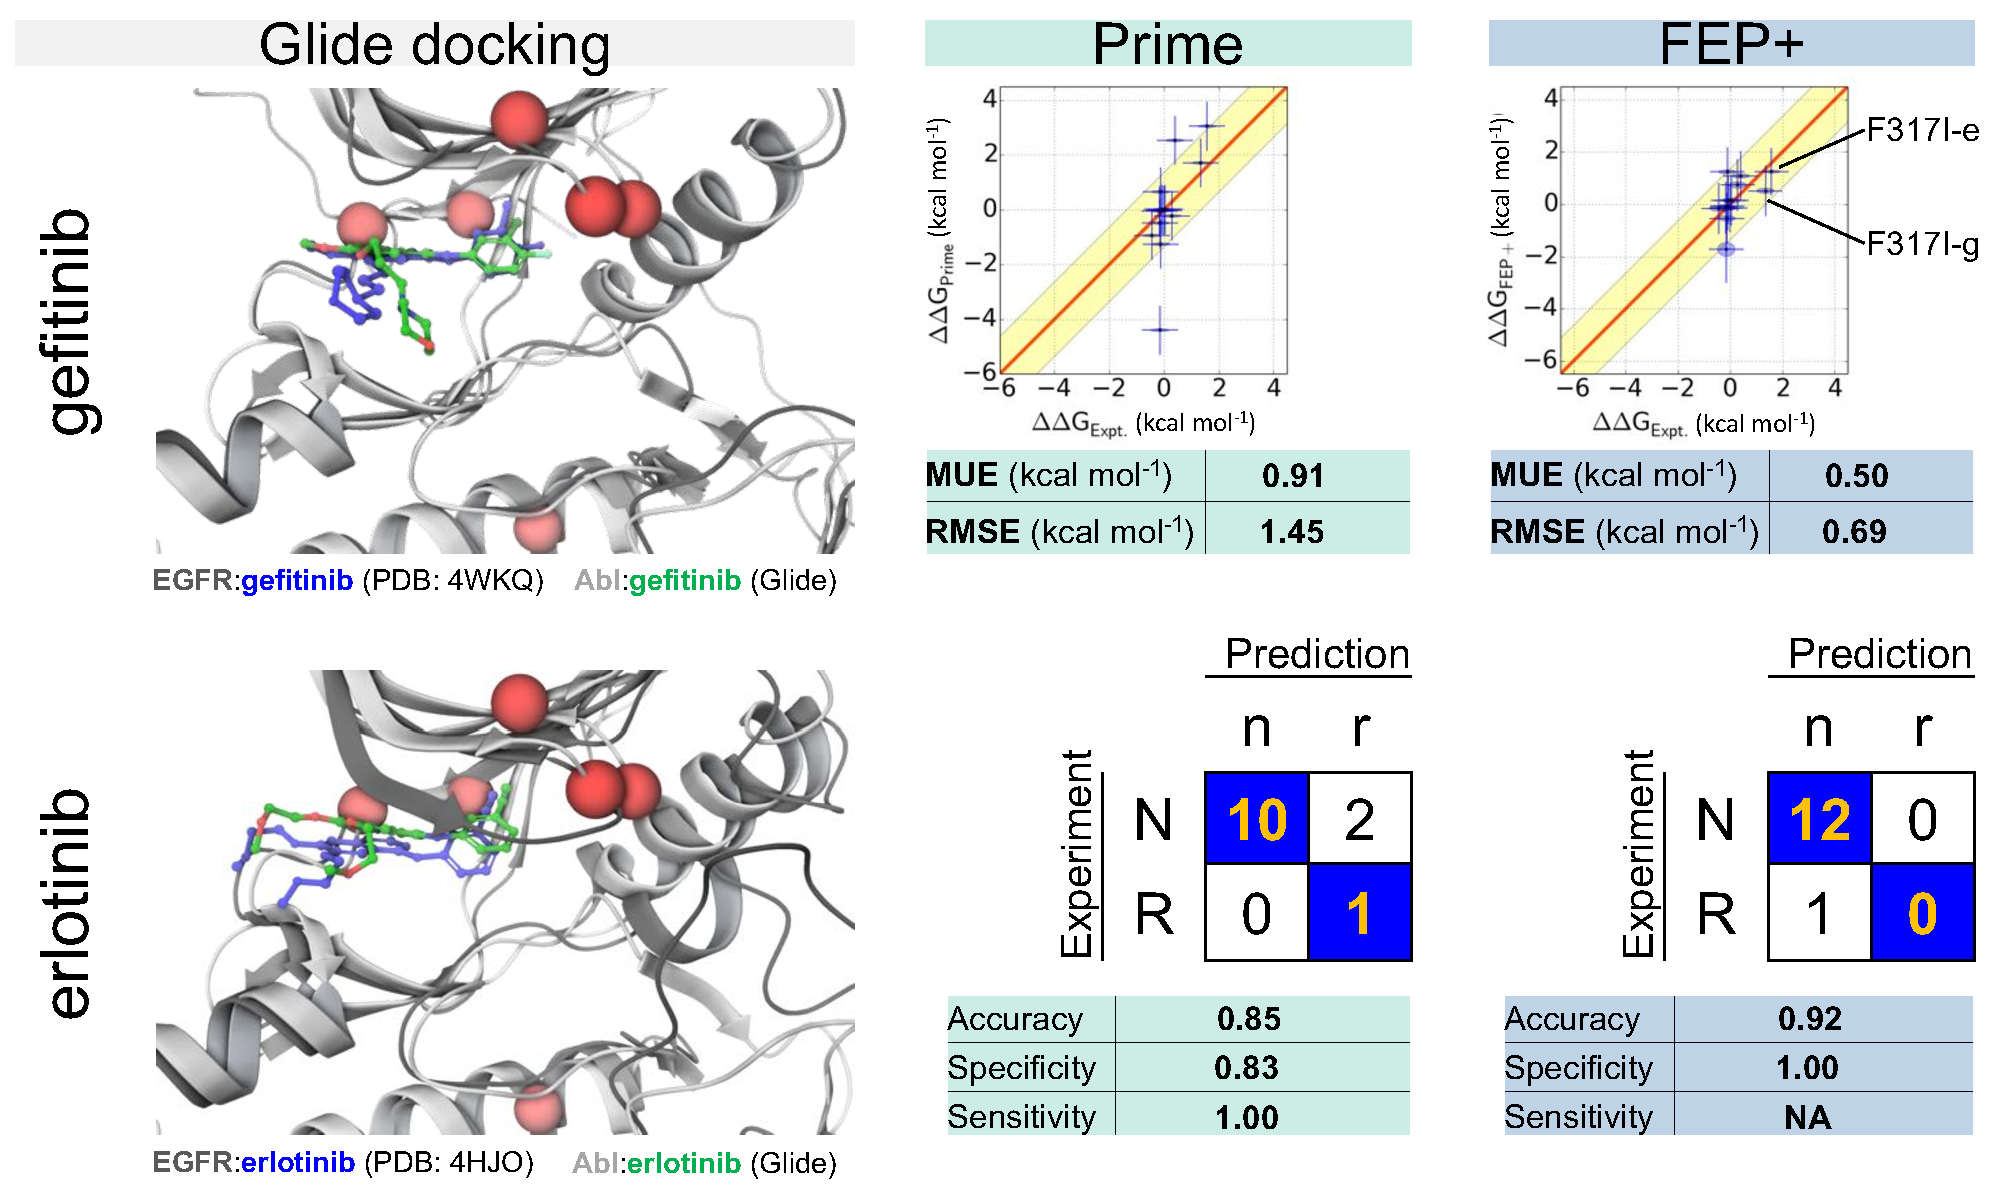
\includegraphics[width=0.8\linewidth]{figures/abl-figure-5.pdf}
		\caption[Predicting resistance mutations using FEP+ for inhibitors for which co-crystal structures with wild-type kinase are not available.]{
			{\bf Predicting resistance mutations using FEP+ for inhibitors for which co-crystal structures with wild-type kinase are not available.}
			The docked pose of Abl:erlotinib is superimposed on the co-crystal structure of EGFR:erlotinib; erlotinib docked to Abl (light gray) is depicted in green and erlotinib bound to EGFR (dark gray) is depicted in blue. 
			The docked pose of Abl:gefitinib is superimposed on the co-crystal structure of EGFR:gefitinib; gefitinib docked to Abl (light gray) is depicted in green and gefitinib bound to EGFR (dark gray) is depicted in blue. The locations of clinical mutants for each inhibitor are highlighted (red spheres).
			The overall RMSEs and MUEs for Prime (center) and FEP+ (right) and two-class accuracies are also shown in the figure.
			Computed free energy changes due to the F317I mutation for erlotinib (-e) and gefitinib (-g) are highlighted in the scatter plot.
			FEP+ results are based on the docked models prepared with crystal waters added back while the Prime (an implicit solvent model) results are based on models without crystallographic water.
		}
		\label{fig:abl-figure5}
	\end{figure}
\end{landscape}

\section{Discussion}

\subsection{Physics-based modeling can reliably predict when a mutation elicits resistance to therapy}
The results presented in this work are summarized in Table~\ref{tab:abl-table-2}.
The performance metrics summarized in Table~\ref{tab:abl-table-2} indicates that the set of 131 mutations for the six TKIs in which co-crystal structures were available is on par with the complete set (144 mutations), which included results based on Abl:TKI complexes generated from docking models.
The performance results for the 13 mutations for the two TKIs (erlotinib and gefitinib) in which co-crystal structures were unavailable exhibited good quantitative accuracy (MUE and RMSE) and good classification power.    

Overall (N=144), the MM-GBSA approach Prime classified mutations with good accuracy ($0.73^{0.80}_{0.66}$) and specificity ($0.76^{0.84}_{0.69}$)
while the alchemical approach FEP+ was a significant improvement in classification accuracy ($0.88^{0.93}_{0.82}$) and specificity ($0.94^{0.98}_{0.89}$).
The quantitative accuracy with which Prime was able to predict the experimentally measured change in Abl:TKI binding (N=142) characterized by RMSE and MUE was $1.70^{1.98}_{1.40}$ kcal mol$^{-1}$ and $1.14^{1.35}_{0.93}$ kcal mol$^{-1}$ respectively.
In stark contrast, the quantitative accuracy of FEP+ was statistically superior to Prime with an RMSE and an MUE of $1.07^{1.26}_{0.89}$ kcal mol$^{-1}$ and $0.79^{0.92}_{0.67}$ kcal mol$^{-1}$ respectively.

From the perspective of a clinician, classification rate would be an important metric to measure the predictive power of technologies such as Prime and FEP+. To test the hypothesis that reducing the large spread in Prime predictions could improve its classification rate, we scaled the computed relative free energies %(by 1/2, 1/3, and by 0.23, which was the optimal factor that gives lowest RMSE) 
and recalculated the performance metrics (Data shown in publication~\citep{Hauser:2018vz}). As expected, the MUE and RMSE were improved but the specificity of Prime was drastically diminished. %; as MUE and RMSE improved, it became increasingly unable to identify resistance mutations. 
Scaling FEP+ eliminated its sensitivity and a na{\"i}ve model (all $\Delta\Delta$Gs = 0.00 kcal mol$^{-1}$) had zero sensitivity. Lastly, we constructed a consensus model in which free energies were a weighted average of scaled Prime and FEP+. This model also had zero sensitivity. %It appears difficult to improve upon the predictive power of FEP+ by statistical operations.

To address the impact of picking a cutoff to classify predicted free energies as resistant or sensitizing, we computed ROC curves for the various predicted datasets: Prime, FEP+, na{\"i}ve model, and consensus model (Data shown in publication~\citep{Hauser:2018vz}). ROC curves and ROC-AUCs for scaled and non-scaled Prime were identical, as well as scaled and non-scaled FEP+, because ROC curves are independent of a linear transformation on the data. %ROC curves for these six sets of predictions are presented in Supplementary \FIG{figure-si-3}. 
ROC-AUC for FEP+ was $0.75_{0.61}^{0.90}$ (n=144); ROC-AUC for Prime was $0.66_{0.52}^{0.81}$ (n=144); ROC-AUCs for the na{\"i}ve model and consensus model were $0.50_{0.50}^{0.50}$ (n=144) and $0.78_{0.67}^{0.90}$ (n=144) respectively. These results show that Prime has poor discriminatory power (ROC-AUC in [0.6,0.7]) while FEP+ has fair discriminatory power (ROC-AUC in [0.7,0.8]).

\begin{landscape}
\begin{table}[p]
	\caption[Summary of FEP+ and Prime statistics in predicting mutational resistance or sensitivity to FDA-approved TKI]{
		\label{tab:abl-table-2} 
		{\bf Summary of FEP+ and Prime statistics in predicting mutational resistance or sensitivity to FDA-approved TKIs}
	}
	% Use "S" column identifier to align on decimal point 
	\setlength{\tabcolsep}{4pt}
	\begin{tabularx}{\linewidth}{X X | c X X | c X X X}
		\toprule
		Dataset		&Method		& N$_\mathrm{quant}$ &  MUE				   & RMSE					& N$_\mathrm{class}$ & Accuracy			& Specificity		& Sensitivity			\\
		&			&   &  (kcal mol$^{-1}$)		   & (kcal mol$^{-1}$)				& 	& 		 		& 					&		 			\\
		\midrule
		all & FEP+ & 142 & $0.79_{0.67}^{0.92}$ & $1.07_{0.89}^{1.26}$ & 144 & $0.88_{0.82}^{0.93}$ & $0.94_{0.89}^{0.98}$ & $0.47_{0.25}^{0.69}$ \\ 
		all & Prime & 142 & $1.14_{0.93}^{1.35}$ & $1.70_{1.40}^{1.98}$ & 144 & $0.73_{0.66}^{0.80}$ & $0.76_{0.69}^{0.84}$ & $0.53_{0.30}^{0.76}$ \\ 
		xtals & FEP+ & 129 & $0.82_{0.69}^{0.95}$ & $1.11_{0.91}^{1.30}$ & 131 & $0.87_{0.81}^{0.92}$ & $0.93_{0.88}^{0.97}$ & $0.50_{0.29}^{0.74}$ \\ 
		xtals & Prime & 129 & $1.16_{0.96}^{1.37}$ & $1.72_{1.41}^{2.00}$ & 131 & $0.72_{0.64}^{0.79}$ & $0.75_{0.67}^{0.83}$ & $0.50_{0.25}^{0.73}$ \\ 
		axitinib & FEP+ & 26 & $0.70_{0.50}^{0.93}$ & $0.91_{0.64}^{1.14}$ & 26 & $0.85_{0.69}^{0.96}$ & $0.85_{0.69}^{0.96}$ & $NA$ \\ 
		axitinib & Prime & 26 & $1.05_{0.53}^{1.71}$ & $1.85_{0.96}^{2.61}$ & 26 & $0.88_{0.73}^{1.00}$ & $0.88_{0.73}^{1.00}$ & $NA$ \\ 
		bosutinib & FEP+ & 21 & $0.96_{0.55}^{1.42}$ & $1.41_{0.77}^{1.97}$ & 21 & $0.76_{0.57}^{0.95}$ & $0.88_{0.71}^{1.00}$ & $0.25_{0.00}^{1.00}$ \\ 
		bosutinib & Prime & 21 & $1.13_{0.60}^{1.83}$ & $1.80_{0.92}^{2.62}$ & 21 & $0.81_{0.62}^{0.95}$ & $0.82_{0.62}^{1.00}$ & $0.75_{0.00}^{1.00}$ \\ 
		dasatinib & FEP+ & 20 & $0.76_{0.49}^{1.13}$ & $1.07_{0.59}^{1.57}$ & 21 & $0.90_{0.76}^{1.00}$ & $0.94_{0.79}^{1.00}$ & $0.80_{0.33}^{1.00}$ \\ 
		dasatinib & Prime & 20 & $1.05_{0.61}^{1.54}$ & $1.48_{0.95}^{1.92}$ & 21 & $0.86_{0.71}^{1.00}$ & $0.88_{0.69}^{1.00}$ & $0.80_{0.33}^{1.00}$ \\ 
		imatinib & FEP+ & 20 & $0.82_{0.53}^{1.15}$ & $1.09_{0.69}^{1.43}$ & 21 & $0.86_{0.71}^{1.00}$ & $1.00_{1.00}^{1.00}$ & $0.40_{0.00}^{0.83}$ \\ 
		imatinib & Prime & 20 & $1.32_{0.91}^{1.81}$ & $1.69_{1.15}^{2.26}$ & 21 & $0.43_{0.24}^{0.67}$ & $0.50_{0.25}^{0.75}$ & $0.20_{0.00}^{0.67}$ \\ 
		nilotinib & FEP+ & 21 & $0.82_{0.57}^{1.12}$ & $1.06_{0.69}^{1.39}$ & 21 & $0.86_{0.67}^{1.00}$ & $0.94_{0.80}^{1.00}$ & $0.50_{0.00}^{1.00}$ \\ 
		nilotinib & Prime & 21 & $1.50_{1.06}^{1.97}$ & $1.86_{1.43}^{2.25}$ & 21 & $0.48_{0.24}^{0.67}$ & $0.53_{0.29}^{0.75}$ & $0.25_{0.00}^{1.00}$ \\ 
		ponatinib & FEP+ & 21 & $0.87_{0.62}^{1.16}$ & $1.09_{0.70}^{1.46}$ & 21 & $1.00_{1.00}^{1.00}$ & $1.00_{1.00}^{1.00}$ & $NA$ \\ 
		ponatinib & Prime & 21 & $0.94_{0.50}^{1.54}$ & $1.57_{0.69}^{2.44}$ & 21 & $0.81_{0.62}^{0.95}$ & $0.81_{0.62}^{0.95}$ & $NA$ \\ 
		Glide & FEP+ & 13 & $0.50_{0.26}^{0.78}$ & $0.69_{0.35}^{0.97}$ & 13 & $0.92_{0.77}^{1.00}$ & $1.00_{1.00}^{1.00}$ & $0.00_{0.00}^{0.00}$ \\ 
		Glide & Prime & 13 & $0.91_{0.39}^{1.56}$ & $1.45_{0.54}^{2.22}$ & 13 & $0.85_{0.62}^{1.00}$ & $0.83_{0.58}^{1.00}$ & $1.00_{0.00}^{1.00}$ \\
		\bottomrule
	\end{tabularx}
	\small
	\smallskip
	\\
	{N$_\mathrm{quant}$}: Number of mutations for which quantitative metrics were evaluated;
	{N$_\mathrm{class}$}: Number mutations for which classification metrics were evaluated;
	{All}: All mutations;
	{xtals}: All mutations for which co-crystal structures were available;
	{Glide}: erlotinib and gefitinib\\
	Accuracy, specificity, and sensitivity were computed to assess two-class prediction performance:\\
	\emph{resistant} ($\Delta \Delta$G > 1.36 kcal mol$^{-1}$) or \emph{susceptible} ($\Delta \Delta$G $\le$ 1.36 kcal mol$^{-1}$).\\
	95\% CIs (sub-/superscripts) were estimated from 1000 bootstrap replicates.
	Note: The sensitivity for axitinib and ponatinib is NA, because there is no resistant mutation for these two drugs.
\end{table}
\end{landscape}

\subsection{Hierarchical Bayesian model estimates global performance}
A hierarchical Bayesian approach was developed to estimate the intrinsic accuracy of the models when the noise in the experimental and predicted values of $\Delta\Delta$G was accounted for.
Utilizing this approach, the MUE and RMSE for Prime was found to be $1.39^{1.58}_{1.23}$ kcal mol$^{-1}$ and $1.75^{1.98}_{1.55}$ kcal mol$^{-1}$ (N=142) respectively.
The accuracy, specificity, and sensitivity of Prime was found using this method to be $0.74^{0.76}_{0.71}$, $0.75^{0.77}_{0.73}$, and $0.59^{0.78}_{0.40}$ (N=144) respectively.
The MUE and RMSE of FEP+ was found to be $0.76^{0.87}_{0.66}$ kcal mol$^{-1}$ and $0.95^{1.09}_{0.82}$ kcal mol$^{-1}$ (N=142) respectively, which is significantly better than Prime.
Likewise, a clearer picture of the true classification accuracy, specificity, and sensitivity of FEP+ was found---$0.90^{0.93}_{0.86}$, $0.92^{0.95}_{0.90}$, and $0.68^{1.00}_{0.46}$ respectively.

The high accuracy of FEP+ is very encouraging, and the accuracy can be further improved with more accurate modeling of a number of physical chemical effects not currently considered by the method. 
While highly optimized, the fixed-charged OPLS3~\citep{Harder:J.Chem.TheoryComput.:2016} force field can be further improved by explicit consideration of polarizability effects~\citep{zotero-1853851-9627}, as hinted by some small-scale benchmarks ~\citep{Jiao:Proc.Natl.Acad.Sci.:2008}.
These features could be especially important for bosutinib, whose 2,4-dichloro-5-methoxyphenyl ring is adjacent to the positively charged amine of the catalytic Lys271.
Many simulation programs also utilize a long-range isotropic analytical dispersion correction intended to correct for the truncation of dispersion interactions at finite cutoff, which can induce an error in protein-ligand binding free energies that depends on the number of ligand heavy atoms being modified~\citep{Shirts:J.Phys.Chem.B:2007}; recently, efficient Lennard-Jones PME methods~\citep{Essmann:J.Chem.Phys.:1995,Wennberg:J.Chem.TheoryComput.:2013} and perturbation schemes~\citep{Shirts:J.Phys.Chem.B:2007} have been developed that can eliminate the errors associated with this truncation.
While the currently employed methodology for alchemical transformations involving a change in system charge (see Methods) reduces artifacts that depend on the simulation box size and periodic boundary conditions, the explicit ions that were included in these simulations may not have sufficiently converged to their equilibrium distributions in these relatively short simulations.
Kinases and their inhibitors are known to possess multiple titratable sites with either intrinsic or effective p$K_{a}$s near physiological pH, while the simulations here treat protonation states and proton tautomers fixed throughout the bound and unbound states; the accuracy of the model can be further improved with the protonation states or tautomers shift  upon binding or mutation considered~\citep{Onufriev:Q.Rev.Biophys.:2013,Martin:2009:JournalofComputer-AidedMolecularDesign}.
Similarly, some systems display significant salt concentration dependence~\citep{Jensen:Curr.Pharm.Biotechnol.:2008a}, while the simulations for some systems reported here did not rigorously mimic all aspects of the experimental conditions of the cell viability assays.

\subsection{Experimentally observed IC$_{50}$ changes can be caused by other physical mechanisms}
While we have shown that predicting the direct impact of mutations on the binding affinity of ATP-competitive tyrosine kinase inhibitors for a single kinase conformation has useful predictive capacity, many additional physical effects that can contribute to cell viability are not currently captured by examining only the predicted change in inhibitor binding affinity.
For example, kinase missense mutations can also shift the populations of kinase conformations (which may affect ATP and inhibitor affinities differentially), modulate ATP affinity, modulate affinity for protein substrate, or modulate the ability of the kinase to be regulated or 
bounded by scaffolding proteins. 
%These physical mechanisms might affect the IC$_{50}$s of cell viability assays but not necessarily the binding affinity of the inhibitors.
While many of these effects are in principle tractable by physical modeling in general %(and alchemical free energy methods in particular), 
it is valuable to examine our mispredictions and outliers to identify whether any of these cases are likely to induce resistance (as observed by $\Delta$pIC$_{50}$ shifts) by one of these alternative mechanisms.


\subsection{Other physical mechanisms of resistance are likely similarly computable.}
A simple threshold of 10-fold TKI affinity change is a crude metric for classifying resistance or susceptibility due to the myriad biological factors that contribute to the efficacy of a drug in a person. 
Except for affecting the binding affinity of inhibitors, missense mutations can also cause drug resistance through other physical mechanisms including induction of splice variants or alleviation of feedback.
While the current study only focused on the effect of mutation on drug binding affinity, resistance from these other physical mechanisms could be similarly computed using physical modeling.
For example, some mutations are known to activate the kinase by increasing affinity to ATP, which could be computed using free energy methods like FEP. %the same thermodynamic cycle utilized here for inhibitors.



%
%
%  CONCLUSION
%
%
%TC:break Conclusion
\section{Conclusion}
Revolutionary changes in computing power---especially the arrival of inexpensive graphics processors (GPUs)---and software automation have enabled alchemical free-energy calculations to impact drug discovery and life sciences projects in previously unforeseen ways.
In this communication, we tested the hypothesis that FEP+, a fully-automated relative-alchemical free-energy workflow,     
had reached the point where it can accurately and reliably predict how clinically-observed mutations in Abl kinase alter the binding affinity of eight FDA-approved TKIs.
To establish the potential predictive impact of current-generation alchemical free energy calculations---which incorporate entropic and enthalpic effects and the discrete nature of aqueous solvation---compared to a simpler physics-based approach that also uses modern forcefields but scores a single minimized conformation, we employed a second physics-based approach (Prime).
This simpler physics-based model, which uses an implicit model of solvation to score the energetic changes in interaction energy that arise from the mutation, was able to capture a useful amount of information to achieve substantial predictiveness with an MUE of $1.14^{1.35}_{0.93}$ kcal mol$^{-1}$ (N=142), RMSE of $1.70^{1.98}_{1.40}$ kcal mol$^{-1}$ respectively (N=142), and classification accuracy of $0.73^{0.80}_{0.66}$ (N=144).
Surpassing these good results, we went on to demonstrate that FEP+ is able to achieve superior predictive performance---
MUE of $0.79^{0.92}_{0.67}$ kcal mol$^{-1}$ (N=142), RMSE of $1.07^{1.26}_{0.89}$ kcal mol$^{-1}$ (N=142), and
classification accuracy of 
$0.88^{0.93}_{0.82}$ (N=144).
While future enhancements to the workflows for Prime and FEP+ to account for additional physical and chemical effects are likely to improve predictive performance further, the present results are of sufficient quality and achievable on a sufficiently rapid timescale (with turnaround times 
$\sim$6 hours/calculation)
to impact research projects in drug discovery and the life sciences.
%With exponential improvements in computing power, we anticipate the domains of applicability for alchemical free-energy methods such as FEP+ will take on increasingly integrated roles to impact projects.
This work illustrates how the domain of applicability for alchemical free-energy methods is much larger than previously appreciated, and might further be found to include new areas as research progresses: aiding clinical decision-making in the selection of first- or second-line therapeutics guided by knowledge of likely subclonal resistance; identifying other selective kinase inhibitors (or combination therapies) to which the mutant kinase is susceptible; supporting the selection of candidate molecules to advance to clinical trials based on anticipated activity against likely mutations; facilitating the enrollments of patients in mechanism-based basket trials; and generally augmenting the armamentarium of precision oncology.

\section{Methods}
\label{sec:methods}

\subsection{System preparation}
All system preparation utilized the Maestro Suite (Schr\"{o}dinger) version 2016-4. 
Comparative modeling to add missing residues using a homologous template made use of the Splicer tool, while missing loops modeled without a template used Prime. 
All tools employed default settings unless otherwise noted.
The Abl wild-type sequence used in building all Abl kinase domain models utilized the ABL1\_HUMAN Isoform IA (P00519-1) UniProt gene sequence spanning S229--K512.
Models were prepared in non-phosphorylated form.
We used a residue indexing convention that places the Thr gatekeeper residue at position 315 to match common usage; an alternate indexing convention utilized in experimental X-ray structures for Abl:imatinib (PDB: 1OPJ) \citep{Nagar:Cell:2003} and Abl:dasatinib (PDB: 4XEY) \citep{Lorenz:Biochem.J.:2015} was adjusted to match our convention. 

\subsubsection{Complexes with co-crystal structures.}

Chain B of the experimental structure of Abl:axitinib (PDB: 4WA9) \citep{Pemovska:Nature:2015} was used, and four missing residues at the N- and C-termini were added using homology modeling with PDB 3IK3 \citep{OHare:CancerCell:2009} as the template following alignment of the respective termini of the kinase domain. Chain B was selected because chain A was missing an additional 3 and 4 residues at the N- and C-termini, respectively, in addition to 3- and 20-residue loops, both of which were resolved in chain B. All missing side chains were added with Prime.
The co-crystal structure of Abl:bosutinib (PDB: 3UE4) \citep{Levinson:PLoSONE:2012a} was missing 4 and 10 N- and C-terminal residues respectively in chain A that were built using homology modeling with 3IK3 as the template. All loops were resolved in chain A (chain B was missing two residues in the P-loop, Q252 and Y253). All missing side chains were added with Prime.
The co-crystal structure of Abl:dasatinib (PDB: 4XEY) \citep{Lorenz:Biochem.J.:2015} was missing 2 and 9 N- and C-terminal residues, respectively, that were built via homology modeling using 3IK3 as the template. A 3 residue loop was absent in chain B but present in chain A; chain A was chosen.
The co-crystal structure of Abl:imatinib (PDB: 1OPJ) \citep{Nagar:Cell:2003} had no missing loops. Chain B was used because chain A was missing two C-terminal residues that were resolved in chain B. A serine was present at position 336 (index 355 in the PDB file) and was mutated to asparagine using Prime to match the human wild-type reference sequence (P00519-1).
The co-crystal structure of Abl:nilotinib (PDB: 3CS9) \citep{Weisberg:CancerCell:2005} contained four chains in the asymmetric unit all of which were missing at least one loop. Chain A was selected because its one missing loop involved the fewest number of residues of the four chains; chain A was missing 4 and 12 N- and C-terminal residues, respectively, that were built using homology modeling with 3IK3 as the template. A 4-residue loop was missing in chain A (chain B and C were missing two loops, chain D was missing a five residue loop) that was built using Prime.
The co-crystal structure of Abl:ponatinib (PDB: 3OXZ) \citep{Zhou:Chem.Biol.DrugDes.:2011} contained only one chain in the asymmetric unit. It had two missing loops, one 4 residues (built using Prime) and one 12 residues (built using homology modeling with 3OY3 \citep{Zhou:Chem.Biol.DrugDes.:2011} as the template). Serine was present at position 336 and was mutated to Asn using Prime to match the human wild-type reference sequence (P00519-1).
Once the residue composition of the six Abl:TKI complexes were normalized to have the same sequence, the models were prepared using Protein Preparation Wizard. Bond orders were assigned using the Chemical Components Dictionary and hydrogen atoms were added. Missing side chain atoms were built using Prime. Termini were capped with N-acetyl (N-terminus) and N-methyl amide (C-terminus). If present, crystallographic water molecules were retained. Residue protonation states (e.g. Asp381 and Asp421) were determined using PROPKA \citep{Li:ProteinsStruct.Funct.Bioinforma.:2005} with a pH range of 5.0--9.0.
Ligand protonation state was assigned using PROPKA with pH equal to the experimental assay.
Hydrogen bonds were assigned by sampling the orientation of crystallographic water, Asn and Gln flips, and His protonation state.
The positions of hydrogen atoms were minimized while constraining heavy atoms coordinates. 
Finally, restrained minimization of all atoms was performed in which a harmonic positional restraint (25.0 kcal mol$^{-1}$ {\AA}$^{-2}$) was applied only to heavy atoms. Table \ref{tab:abl-table-si-9} summarizes the composition of the final models used for FEP.

\begin{landscape}
\begin{table}
	\footnotesize
	\caption[Summary of the preparation of the 6 Abl:TKI co-crystal structure complexes]{ 
		\label{tab:abl-table-si-9}
		{\bf Summary of the preparation of the 6 Abl:TKI co-crystal structure complexes}
	}
	\setlength{\tabcolsep}{4pt}
	%               1 2 3 4 5 6 7 8 9 0 1 2 3 4 5 6
	\begin{tabular}{l l l l c c c c r r r r r r r r}
		\toprule
		&				&			& \multicolumn{4}{c}{Experimental structure}	& \multicolumn{9}{c}{Prepared model used for simulations} \\
		\toprule
		{\bf PDB}	& {\bf Receptor}	& {\bf Ligand}	& {\bf Chains}	& {\bf \# Water}$^{a}$	& {\bf \# Rec. atoms,}	& {\bf \# Aminos,}	& {\bf Chain}	& {\bf \# Water}	& {\bf \# Rec.}	& {\bf \# Rec.}	& {\bf \# Ash}	& {\bf \# Glh}	& {\bf \# Hip}	& {\bf \# Lig.}	& {\bf Het. atom}$^{d}$ 	\\
		& 				& 			& 			& 					& {(Chain)}	$^{b}$	& {(Chain)}		& {used}	& 				& {atoms}	& {aminos}	& 			& 			& 			& {atoms}	& {w/ proton}		\\
		\toprule
		4wa9	& {Abl}	& {Axit}	& {A, B}		& {305}	& {2219 (B)}	& {276 (B)}	& {B}	& {131}	& {4580}	& {284}	& {Ash421}			& {0}	& {0}	& {46}	& {neutral} 		\\
		3ue4	& {Abl}	& {Bosut}	& {A, B}		& {152}	& {2187 (A)}	& {270 (A)}	& {A}	& {89}	& {4581}	& {284}	& {Ash421}			& {0}	& {0}	& {66}	& {NBI,4401} 		\\
		& {}	& {}		& {}			& {}	& {}			& {}		& {}	& {}	& {}		& {}	& {Ash381}			& {}	& {}	& {}	& {} 		\\
		4xey	& {Abl}	& {Dasat}	& {A, B}		& {0}	& {2195 (A)}	& {269 (A)}	& {A}	& {0}	& {4581}	& {284}	& {Ash421$^{c}$}		& {0}	& {0}	& {59}	& {neutral} 		\\
		& {}	& {}		& {}			& {}	& {}			& {}		& {}	& {}	& {}		& {}	& {Ash381$^{c}$}	& {}	& {}	& {}	& {} 		\\
		1opj	& {Abl}	& {Imat}	& {A, B}		& {231}	& {2336 (B)}	& {288 (B)}	& {B}	& {104}	& {4579}	& {284}	& {0}				& {0}	& {0}	& {69}	& {N51,4767} 		\\
		3cs9	& {Abl}	& {Nilot}	& {A, B, C, D}	& {266}	& {2142 (A)}	& {264 (A)}	& {A}	& {99}	& {4579}	& {284}	& {0}				& {0}	& {0}	& {61}	& {neutral} 		\\
		3oxz	& {Abl}	& {Ponat}	& {A}			& {89}	& {2152 (A)}	& {268 (A)}	& {A}	& {89}	& {4580}	& {284}	& {0}				& {0}	& {0}	& {67}	& {N3,2155} 		\\
		\bottomrule
	\end{tabular}
	\\
	\medskip 
	\\
	\small
	\\
	$^{a}$Total number of water molecules, %\\
	$^{b}$Count includes N-Acetyl/N-terminal (6 atoms) and N-methylamide/C-terminal (6 atoms) capping groups, %\\
	$^{c}$Original index in experimental structure was Ash440, Ash400, %\\
	$^{d}$(PDB atom name) and (PDB atom serial number).\\
	\textbf{Ash}: Neutral form of Asp; \textbf{Glh}: Neutral form of Glu; \textbf{Hip}: Charged form of His.\\
\end{table}
\end{landscape}

\subsubsection{Complexes without co-crystal structures.}
Co-crystal structures of Abl bound to erlotinib or gefitinib were not publicly available. To generate models of these complexes, Glide-SP~\citep{Friesner:J.Med.Chem.:2004} was utilized to dock these two compounds into an Abl receptor structure. 
Co-crystal structures of these two compounds bound to EGFR were publicly available and this information was used to obtain initial ligand geometries and to establish a reference binding mode against which our docking results could be structurally scored.    
The Abl receptor structure bound to bosutinib was used for docking because its structure was structurally similar to that of EGFR in the erlotinib- (PDB: 4HJO) \citep{Park:Biochem.J.:2012} and gefitinib-bound (PDB: 4WKQ) \citep{Yosaatmadja::2014} co-crystal structures. 
Abl was prepared for docking by using the Protein Preparation Wizard (PPW) with default parameters. 
Crystallographic waters were removed but their coordinates retained for a subsequent step in which they were optionally reintroduced. 
Erlotinib and gefitinib protonation states at pH 7.0$\pm$2.0 were determined using Epik~\citep{Shelley:J.Comput.AidedMol.Des.:2007}.
Docking was performed using the Glide-SP workflow. 
The receptor grid was centered on bosutinib. 
The backbone NH of Met318 was chosen to participate in a hydrogen bonding constraint with any hydrogen bond donor on the ligand. 
The hydroxyl of T315 was allowed to rotate in an otherwise rigid receptor. Ligand docking was performed with enhanced sampling; otherwise default settings were used. Epik state penalties were included in the scoring. The 16 highest ranked (Glide-SP score) poses were retained for subsequent scoring. 
To determine the docked pose that would be subsequently used for free energy calculations, the ligand heavy-atom RMSD between the 16 poses and the EGFR co-crystal structures (PDB IDs 4HJO and 4WKQ) was determined. 
The pose in which erlotinib or gefitinib most structurally resembled the EGFR co-crystal structure (lowest heavy-atom RMSD) was chosen as the pose for subsequent FEP+. 
Two sets of complex structures were subjected to free energy calculations to determine the effect of crystal waters: In the first set, without crystallographic waters, the complexes were prepared using Protein Prep Wizard as above. 
In the second set, the crystallographic waters removed prior to docking were added back, and waters in the binding pocket that clashed with the ligand were removed. 

\subsection{Force field parameter assignment}
The OPLS3 forcefield~\citep{Harder:J.Chem.TheoryComput.:2016} version that shipped with Schr\"{o}dinger Suite release 2016-4 was used to parameterize the protein and ligand.
Torsion parameter coverage was checked for all ligand fragments using Force Field Builder. 
The two ligands that contained a fragment with a torsion parameter not covered by OPLS3 were axitinib and bosutinib; Force Field Builder was used to obtain these parameters. 
SPC parameters~\citep{Berendsen:IntermolecularForces:1981} were used for water. For mutations that change the net change of the system, counterions were included to neutralize the system with additional Na+ and Cl- ions added to achieve 0.15 M excess to mimic the solution conditions of the experimental assay.

\subsection{Prime (MM-GBSA)}
Prime was used to predict the geometry of mutant side chains and to calculate relative changes in free energy using MM-GBSA single-point estimates \citep{Rapp:J.Chem.Inf.Model.:2011}. VSGB \citep{Shivakumar:J.Chem.TheoryComput.:2010} was used as the implicit solvent model to calculate the solvation free energies for the four states (complex/wild-type, complex/mutant, apo protein/wild-type, and apo protein/mutant) and $\Delta\Delta$G calculated using the thermodynamic cycle depicted in Figure~\ref{fig:abl-figure1}B. 
Unlike FEP (see below), which simulates the horizontal legs of the thermodynamic cycle, MM-GBSA models the vertical legs by computing the interaction energy between the ligand and protein in both wild-type and mutant states, subtracting these to obtain the $\Delta\Delta$G of mutation on the binding free energy.

\subsection{Alchemical free energy perturbation calculations using FEP+}
Alchemical free energy calculations were performed using the FEP+ tool in the Schr\"{o}dinger Suite version 2016-4, which offers a fully automated workflow requiring only an input structure (wild-type complex) and specification of the desired mutation. 
The default protocol was used throughout: It assigns protein and ligand force field parameters (as above), generates a dual-topology~\citep{Pearlman:J.Phys.Chem.:1994} alchemical system for transforming wild-type into mutant protein (whose initial structure is modeled using Prime), generates the solvent-leg endpoints (wild-type and mutant apo protein), and constructs intermediate  windows spanning wild-type and mutant states. 
Simulations of the apo protein were setup by removing the ligand from the prepared complex (see System Preparation) followed by an identical simulation protocol as that used for the complex.
Charge-conserving mutations utilized 12 $\lambda$ windows (24 systems) while charge-changing mutations utilized 24 $\lambda$  windows (48 systems). 
Each system was solvated in an orthogonal box of explicit solvent (SPC water~\citep{Berendsen:IntermolecularForces:1981}) with box size determined to ensure that solute atoms were no less than 5 {\AA} (complex leg) or 10 {\AA} (solvent leg) from an edge of the box. 
For mutations that change the net charge of the system, counterions were included to neutralize the charge of the system, and additional Na+ and Cl- ions added to achieve 0.15~M excess NaCl to mimic the solution conditions of the experimental assay. 
The artifact in electrostatic interactions for charge change perturbations due to periodic boundary conditions in MD simulations are corrected based on the method proposed by Rocklin \textit{et al.}~\citep{Rocklin:J.Chem.Phys.:2013e},
where the difference in solvation free energy of the solute under non-periodic boundary condition and that under periodic boundary condition is approximated by Poisson-Boltzmann method and serves as the correction term for each system.

System equilibration was automated.
It followed the default 5-stage Desmond protocol: 
(i) 100~ps with 1~fs time steps of Brownian dynamics with positional restraints of solute heavy atoms to their initial geometry using a restraint force constant of 50~kcal mol$^{-1}$ {\AA}$^{-2}$; 
this Brownian dynamics integrator corresponds to a Langevin integrator in the limit when $\tau\rightarrow$0, modified to stabilize equilibration of starting configurations with high potential energies; particle and piston velocities were clipped so that particle displacements were limited to 0.1 {\AA}, in any direction.
(ii) 12~ps MD simulations with 1 fs time step using Langevin thermostat at 10 K with constant volume, using the same restraints; 
(iii) 12~ps MD simulations with 1~fs time step using Langevin thermostat and barostat~\citep{langevin-piston} at 10~K and constant pressure of 1 atmosphere, using the same restraints; 
(iv) 12~ps MD simulations with 1~fs time step using Langevin thermostat and barostat at 300~K and constant pressure of 1 atmosphere, using the same restraints; 
(v) a final unrestrained equilibration MD simulation of 240~ps with 2~fs time step using Langevin thermostat and barostat at 300~K and constant pressure of 1 atmosphere.
Electrostatic interactions were computed with particle-mesh Ewald (PME)~\citep{pme} and a 9~{\AA} cutoff distance was used for van de Waals interactions.
The production MD simulation was performed in the NPT ensemble using the MTK method~\citep{mtk} with integration time steps of 4~fs, 4~fs, and 8~fs respectively for the bonded, near, and far interactions following the RESPA method~\citep{respa} through hydrogen mass repartitioning~\citep{hmr}.
Production FEP+ calculations utilized Hamiltonian replica exchange with solute tempering (REST)~\citep{Wang:Proc.Natl.Acad.Sci.:2012}, with automated definition of the REST region. 
Dynamics were performed with constant pressure of 1 atmosphere and constant temperature of 300 K for 5~ns in which exchanges between windows was attempted every 1.2~ps. 

Because cycle closure could not be used to reduce statistical errors via path redundancy~\citep{Wang:Proc.Natl.Acad.Sci.:2012}, we instead performed mutational free energy calculations in triplicate by initializing dynamics with different random seeds. 
The relative free energies for each mutation in each independent run were calculated using BAR~\citep{Bennett:J.Comput.Phys.:1976,Shirts:Phys.Rev.Lett.:2003}
The reported $\Delta\Delta$G was computed as the mean of the computed $\Delta\Delta$G from three independent simulations.
Triplicate simulations were performed in parallel using four NIVIDA Pascal Architecture GPUs per alchemical free-energy simulation (12 GPUs in total), requiring $\sim$6~hours in total to compute $\Delta\Delta$G.    

\subsection{Obtaining $\Delta\Delta$G from $\Delta$pIC$_{50}$ benchmark set data}
Reference relative free energies were obtained from three publicly available sources of $\Delta$pIC$_{50}$ data (Table~\ref{tab:abl-table-1}).
Under the assumption of Michaelis-Menten binding kinetics (pseudo first-order, but relative free energies are likely consistent), the inhibitor is competitive with ATP (\EQ{ic50}). 
This assumption has been successfully used to estimate relative free energies~\citep{Price:Bioorg.Med.Chem.Lett.:2000,Luccarelli:J.Chem.TheoryComput.:2010,Michel:J.Med.Chem.:2006,mondal2016} using the relationship between IC$_{50}$ and competitive inhibitor affinity $K_{i}$,
\begin{equation}
\label{eq:ic50}
\mathrm{IC}_{50} = \frac{ K_{i} }{ 1 + \frac{[S_{0}]}{K_{M}} } .
\end{equation}
If the Michaelis constant for ATP ($K_{M}$) is much larger than the initial ATP concentration $S_{0}$, the relation in \EQ{ic50} will tend towards the equality IC$_{50}$ = $K_{i}$. The relative change in binding free energy of Abl:TKI binding due to protein mutation is simply,
\begin{eqnarray}
\Delta\Delta G = - RT \ln \frac{\mathrm{IC}_{50,WT}}{\mathrm{IC}_{50,mut}} \label{eq:ddg}
\end{eqnarray}
where IC$_{50,WT}$ is the IC$_{50}$ value for the TKI binding to the wild-type protein and IC$_{50,mut}$ is the IC$_{50}$ value for the mutant protein. 
$R$ is the ideal gas constant and $T$ is taken to be room temperature (300~K).

As alluded to above, relating $\Delta$pIC$_{50}$s to $\Delta\Delta$Gs assumes that the Michaelis constant for ATP is much larger than the initial concentration of ATP, and that the experimentally observed $\Delta$pIC$_{50}$ change is solely from changes in kinase:TKI binding affinity. In practice, not all of these assumptions may hold. 
For example, the experimentally observed $\Delta$pIC$_{50}$ might depend on the metabolism of drugs, and for drugs with different mechanisms of action than directly binding to the kinase binding pocket (e.g., binding to the transition structures of kinases, target gene amplification, up-/down-regulation of positive-/negative-feedback effectors, diminished synergism of pro-apoptotic machinery, decoupling of the target from cell survival circuits)~\citep{BarouchBentov:2011dx,McDermott:2007kq},
their inhibition ability might not correlate well with binding affinity. 
However, the comparison between $\Delta$pIC$_{50}$ and $\Delta K_{D}$ is presented in Figure~\ref{fig:abl-figure2}D, and this comparison indicates the assumptions we used to relate $\Delta$pIC$_{50}$ to $\Delta\Delta$G are reasonable for the dataset we studied.

%%%
\subsection{Assessing prediction performance}

\subsubsection{Quantitative accuracy metrics}
Mean unsigned error (MUE) was calculated by taking the average absolute difference between predicted and experimental estimates of $\Delta\Delta$G. 
Root-mean square error (RMSE) was calculated by taking the square root of the average squared difference between predicted and experimental estimates of $\Delta\Delta$G. 
MUE depends linearly on errors such that large and small errors contribute equally to the average value, while RMSE depends quadratically on errors, magnifying their effect on the average value.

\subsubsection{Truth tables}
Two-class truth tables were constructed to characterize the ability of Prime and FEP+ to correctly classify mutations as susceptible ($\Delta\Delta$G $\le$ 1.36 kcal mol$^{-1}$) or resistant ($\Delta\Delta$G $>$ 1.36 kcal mol$^{-1}$), where the 1.36 kcal mol$^{-1}$ threshold represents a 10-fold change in affinity. 
Accuracy was calculated as the fraction of all predictions that were correctly classified as sensitizing, neutral, or resistant.
Sensitivity and specificity were calculated using a binary classification of resistant ($\Delta\Delta$G $>$ 1.36 kcal mol$^{-1}$) or susceptible ($\Delta\Delta$G $\le$ 1.36 kcal mol$^{-1}$). 
Specificity was calculated as the fraction of correctly predicted non-resistant mutations out of all truly susceptible mutations {\bf S}.
Sensitivity was calculated as the fraction of correctly predicted resistant mutations out of all truly resistant mutations, {\bf R}. 
The number of susceptible mutations was 113 for axitinib, bosutinib, dasatinib, imatinib, nilotinib and ponatinib, and 12 for erlotinib and gefitinib; the number of resistant mutations {\bf R} was 18 for axitinib, bosutinib, dasatinib, imatinib, nilotinib, and ponatinib, and 1 for erlotinib and gefitinib.

\subsubsection{Consensus model}
First, Prime and FEP+ (n=142) were scaled by minimizing their RMSE to experiment by optimizing slope using linear regression. The resulting (minimum) RMSE was used in a subsequent step to combine the scaled FEP+ and scaled Prime free energies with inverse-variance weighted averaging.

\subsubsection{ROC}
A ROC curve was generated by computing the true positive rate (sensitivity) and the true negative rate (specificity) when the classification cutoff differentiating resistant from sensitizing mutations is changed for (only) the predicted values of $\Delta\Delta$G. Cutoffs were chosen by taking the minimum and maximum value of $\Delta\Delta$G for a data set (Prime or FEP+), and iteratively computing specificity and sensitivity in steps of 0.001 kcal mol$^{-1}$, which by this definition will be in the range [0,1]. Experimental positives and negatives were classified with the 1.36 kcal mol$^{-1}$ cutoff. ROC-AUC was computed using the trapezoidal rule.

\subsubsection{Estimating uncertainties of physical-modeling results}
95\% symmetric confidence intervals (CI, 95\%) for all performance metrics were calculated using bootstrap by resampling all datasets with replacement, with 1000 resampling events.
Confidence intervals were estimated for all performance metrics and reported as $x_{x_\mathrm{low}}^{x_\mathrm{high}}$ where $x$ is the mean statistic calculated from the complete dataset (e.g.~RMSE), and $x_\mathrm{low}$ and $x_\mathrm{high}$ are the values of the statistic at the $2.5^{th}$ and $97.5^{th}$ percentiles of the value-sorted list of the bootstrap samples.
Uncertainty for $\Delta\Delta$Gs was computed by the standard deviation between three independent runs (using different random seeds to set initial velocities), where the 95\% CI was [$\Delta\Delta$G$-$1.96$\times \sigma _\mathrm{FEP+}$, $\Delta\Delta$G$+$1.96$\times \sigma _\mathrm{FEP+}$] kcal mol$^{-1}$.
1$\sigma$ used in plots for FEP+ and experiment; 0$\sigma$ for Prime.

\subsubsection{Bayesian hierarchical model to estimate intrinsic error}
We used Bayesian inference to estimate the true underlying prediction error of Prime and FEP+ by making use of known properties of the experimental variability (characterized in Figure~\ref{fig:abl-figure2}) and statistical uncertainty estimates generated by our calculations under weak assumptions about the character of the error.

We presume the true free energy differences of mutation $i$, $\Delta\Delta G^\mathrm{true}_i$, comes from a normal background distribution of unknown mean and variance,
\begin{eqnarray}
\Delta \Delta G^\mathrm{true}_i &\sim& \mathcal{N}(\mu_\mathrm{mut}, \sigma_\mathrm{mut}^2) \:\: i = 1, \ldots, M
\end{eqnarray}
where there are $M$ mutations in our dataset.
We assign weak priors to the mean and variance
\begin{eqnarray}
\mu_\mathrm{mut} &\sim& U(-6, +6) \\
\sigma_\mathrm{mut} &\propto& 1
\end{eqnarray}
where we limit $\sigma > 0$.

We presume the true computational predictions (absent statistical error) differ from the (unknown) true free energy difference of mutation $\Delta\Delta G^\mathrm{true}_i$ by normally-distributed errors with zero bias but standard deviation equal to the RMSE for either Prime or FEP+, the quantity we are focused on estimating:
\begin{eqnarray}
\Delta\Delta G_{i, \mathrm{Prime}}^\mathrm{true} &\sim& \mathcal{N}(\Delta\Delta G^\mathrm{true}_i, \mathrm{RMSE}^2_\mathrm{Prime}) \\
\Delta\Delta G_{i, \mathrm{FEP+}}^\mathrm{true} &\sim& \mathcal{N}(\Delta\Delta G^\mathrm{true}_i, \mathrm{RMSE}^2_\mathrm{FEP+})
\end{eqnarray}

In the case of Prime, since the computation is deterministic, we actually calculate $\Delta\Delta G_\mathrm{Prime}^\mathrm{true}$ for each mutant.
For FEP+, however, the computed free energy changes are corrupted by statistical error, which we also presume to be normally distributed with standard deviation $\sigma_{\mathrm{calc},i}$,
\begin{eqnarray}
\Delta\Delta G_{i, \mathrm{FEP+}} &\sim& \mathcal{N}(\Delta\Delta G_{i, \mathrm{FEP+}}, \sigma_{i,\mathrm{FEP+}}^2)
\end{eqnarray}
where $\Delta\Delta G_{i, \mathrm{FEP+}}$ is the free energy computed for mutant $i$ by FEP+, and $\sigma_{i,\mathrm{FEP+}}$ is the corresponding statistical error estimate.

The experimental data we observe is also corrupted by error, which we presume to be normally distributed with standard deviation $\sigma_\mathrm{exp}$:
\begin{eqnarray}
\Delta\Delta G_{i,\mathrm{exp}} &\sim& \mathcal{N}(\Delta\Delta G_i, \sigma_\mathrm{exp}^2)
\end{eqnarray}
Here, we used an estimate of $K_d$- and IC$_{50}$-derived $\Delta \Delta G$ variation derived from the empirical RMSE of 0.81 kcal mol$^{-1}$, where we took $\sigma_\mathrm{exp} \approx 0.81 / \sqrt{2} = 0.57$ kcal mol$^{-1}$ to ensure the difference between two random measurements of the same mutant would have an empirical RMSE of 0.81 kcal mol$^{-1}$.

Under the assumption that the true $\Delta \Delta G$ is normally distributed and the calculated value differs from the true value via a normal error model, it can easily be shown that the MUE is related to the RMSE via
\begin{eqnarray}
\mathrm{MUE} &=& \int dx_\mathrm{true} \, p(x_\mathrm{true}) \int dx_\mathrm{calc} \, p(x_\mathrm{calc} | x_\mathrm{true}) \, | x_\mathrm{calc} - x_\mathrm{true} | \\
&=& \int dx_\mathrm{true} \frac{1}{\sqrt{2 \pi \sigma_\mathrm{true}^2}} e^{-\frac{(x_\mathrm{true} - \mu_\mathrm{true})^2}{2 \sigma_\mathrm{true}^2}} \int dx_\mathrm{calc} \frac{1}{\sqrt{2 \pi \sigma_\mathrm{calc}^2}} e^{-\frac{(x_\mathrm{calc} - \mu_\mathrm{true})^2}{2 \sigma_\mathrm{calc}^2}} | x_\mathrm{calc} - x_\mathrm{true} | \\
&=& \sqrt{\frac{2}{\pi}} \, \mathrm{RMSE} 
\end{eqnarray}

The model was implemented using PyMC3~\citep{pymc3}, observable quantities were set to their computed or experimental values, and 5000 samples drawn from the posterior (after discarding an initial 500 samples to burn-in) using the default NUTS sampler.
Expectations and posterior predictive intervals were computed from the marginal distributions obtained from the resulting traces.


%TC:break Data availability
\subsection{Data availability}
All relevant data are publicly available: compiled experimental datasets, input files for Prime and FEP+ and computational results that support our findings can be found at GitHub by following the URL: \url{https://github.com/kehauser/Predicting-resistance-of-clinical-Abl-mutations-to-targeted-kinase-inhibitors-using-FEP}

%TC:break Code availability
\subsection{Code availability}
Scripts used for statistics analysis (including the Bayesian inference model) can be found at the following URL: \url{https://github.com/kehauser/Predicting-resistance-of-clinical-Abl-mutations-to-targeted-kinase-inhibitors-using-FEP}



%%%%%%%%%%%%%%%%%%%%%%%%%%%%%%%%%%%%%%%%%%%%%%%%%%%%%%%%%%%%
%%% ACKNOWLEDGMENTS
%%%%%%%%%%%%%%%%%%%%%%%%%%%%%%%%%%%%%%%%%%%%%%%%%%%%%%%%%%%%

%TC:break Acknowledgements
\section{Acknowledgments}
We thank Daniel Robinson (Schr\"{o}dinger), Sonya M.\ Hanson (MSKCC), and Gregory A.\ Ross (MSKCC) for helpful discussions.
JDC acknowledges support from NIH National Cancer Institute Cancer Center Core Grant P30 CA008748; JDC and SKA acknowledge support from the Sloan Kettering Institute, Cycle for Survival, and NIH grant R01 GM121505.
KH acknowledges help from Wei Chen (Schr\"{o}dinger) and Anthony Clark (Schr\"{o}dinger) for instructions on running mutations changing the net charge of the system, and Simon Gao (Schr\"{o}dinger) for assistance in computational resources.

%TC:break Disclosures
%%%%%%%%%%%%%%%%%%%%%%%%%%%%%%%%%%%%%%%%%%%%%%%%%%%%%%%%%%%%
%%% AUTHOR CONTRIBUTIONS
%%%%%%%%%%%%%%%%%%%%%%%%%%%%%%%%%%%%%%%%%%%%%%%%%%%%%%%%%%%%
%TC:break Author Contributions
\section{Author Contributions}
KH, JDC, CN, RA, and LW designed the research; 
KH, SA, TS, and LW identified experimental datasets; 
KH and LW performed the simulations; 
KH, CN, SKA, SR, TS, RA, JDC, and LW analyzed the data; 
KH, JDC, SKA, and LW wrote the paper.

%\section{Disclosures}
\section{Competing Interests}
JDC is a member of the Scientific Advisory Board for Schr\"{o}dinger Inc. SR was a former employee of Schr\"{o}dinger Inc.; and KH, CN, RA, TS, and LW are employess of Schr\"{o}dinger Inc.


\chapter{Enabling high-throughput biophysical experiments on clinically-observed mutations}

The work in this chapter was submitted to \emph{Biochemistry} and appeared as: 
\realsinglespacing
\flushleft{\bf An open library of human kinase domain constructs for automated bacterial expression}
\flushleft{{\bf Steven K. Albanese$^{\dag,1,2}$, Daniel L. Parton$^{\dag,2}$, Mehtap Işık$^{\ddag,2,3}$, Lucelenie Rodr\'{i}guez-Laureano$^{\ddag,2}$, Sonya M. Hanson$^2$, Julie M. Behr$^{2,7}$, Scott Gradia$^{\&,4}$, Chris Jeans$^4$,Nicholas M. Levinson$^6$, Markus A. Seeliger$^5$, John D. Chodera$^{2,*}$} \\
	\emph{\normalsize $^1$ Louis V. Gerstner, Jr. Graduate School of Biomedical Sciences, Memorial Sloan Kettering Cancer Center, New York, NY 10065 } \\
	\emph{\normalsize $^2$ Computational and Systems Biology Program, Sloan Kettering Institute, Memorial Sloan Kettering Cancer Center, New York, NY 10065}\\
	\emph{\normalsize $^3$ Tri-Institutional PhD Program in Chemical Biology, Weill Cornell Graduate School of Medical Sciences, Cornell University, New York, NY 10065} \\
	\emph{\normalsize $^4$ QB3 MacroLab, University of California, Berkeley, CA 94720} \\
	\emph{\normalsize $^5$ Department of Pharmacological Sciences, Stony Brook University Medical School, Stony Brook, NY 11794} \\
	\emph{\normalsize $^6$ Department of Pharmacology, University of Minnesota, Minneapolis, MN 55455} \\
	\emph{\normalsize $^7$ Tri-Institutional Program in Computation Biology and Medicine, Weill Cornell Graduate School of Medical Sciences, Cornell University, New York, NY 10065}\\
	\emph{\normalsize $^\dag$ or $\ddag$ These authors contributed equally to this work} \\
	\emph{\normalsize $^*$ Corresponding Author} \\
	\emph{\normalsize $^\&$ Present Address: Caribou Biosciences, Berkeley, CA 94720} \\
}

\realdoublespacing 
\section{Abstract}
Kinases play a critical role in cellular signaling and are dysregulated in a number of diseases, such as cancer, diabetes, and neurodegeneration. 
Therapeutics targeting kinases currently account for roughly 50\% of cancer drug discovery efforts. The ability to explore human kinase biochemistry and biophysics in the laboratory is essential to designing selective inhibitors and studying drug resistance. 
Bacterial expression systems are superior in terms of simplicity and cost-effectiveness compared to insect or mammalian cells, but have historically struggled with human kinase expression.
Following the discovery that phosphatase coexpression produced high yields of Src and Abl kinase domains in bacteria, we have generated a library of 52 His-tagged human kinase domain constructs that express above 2~$\mu$g/mL culture in an automated bacterial expression system utilizing phosphatase coexpression (YopH for Tyr kinases, Lambda for Ser/Thr kinases). 
Here, we report a structural bioinformatics approach to identify kinase domain constructs previously expressed in bacteria and likely to express well in our protocol, experiments demonstrating our simple construct selection strategy selects constructs with good expression yields in a test of 84 potential kinase domain boundaries for Abl, and yields from a high-throughput expression screen of 96 human kinase constructs.
Using a fluorescence-based thermostability assay and a fluorescent ATP-competitive inhibitor, we show that the highest-expressing kinases are folded and have well-formed ATP binding sites.
We also demonstrate that these constructs can enable characterization of clinical mutations by expressing a panel of 48 Src and 46 Abl mutations. 
The wild-type kinase construct library is available publicly via Addgene. 

\section{Introduction}

Kinases play a critical role in cellular signaling pathways, controlling a number of key biological processes that include growth and proliferation. 
There are over 500 kinases in the human genome~\citep{manning:science:2002:kinome,Hunter:ReceptorTyrosineKinases:StructureFunctionsandRoleinHumanDisease:2015}, many of which are of therapeutic interest.
Perturbations due to mutation, translocation, or upregulation can cause one or more kinases to become dysregulated, often with disastrous consequences~\citep{knight_targeting_2010}.
Kinase dysregulation has been linked to a number of diseases, such as cancer, diabetes, and inflammation.
Cancer alone is the second leading cause of death in the United States, accounting for nearly 25\% of all deaths; in 2015, over 1.7 million new cases were diagnosed, with over 580,000 deaths~\citep{acs-cancer-facts-2015}. 
Nearly 50\% of cancer drug development is targeted at kinases, accounting for perhaps 30\% of \emph{all} drug development effort globally~\citep{cohen_will_2010,Santos:Nat.Rev.DrugDiscov.:2016}. 

The discovery of imatinib, an inhibitor that targets the Abelson tyrosine kinase (Abl) dysregulated in chronic myelogenous leukemia (CML) patients,
%by a gene translocation event, which removes a myristoylated N-terminal fragment that mediates a conformational change in a C-terminal alpha helix required for autoinhibition and results in a constitutively active kinase~\citep{Nagar:2003tu}, 
was transformative in revealing the enormous therapeutic potential of selective kinase inhibitors, kindling hope that this remarkable success could be recapitulated for other cancers and diseases~\citep{stegmeier:clpt:2010:imatinib-lessons}.
While there are now 39 FDA-approved selective kinase small molecule inhibitors (as of 16 Jan 2018)~\citep{wu_fda-approved_2015,fda-approved-kinase-inhibitors}, these molecules were approved for targeting only 22 out of $\sim$500 human kinases\footnote{These targets are, currently: Abl, DDR1, EGFR, HER2, VGFR1/2/3, Alk, Met, BRAF, JAK1/2/3, Btk, Pi3K, CDK4, CDK6, MEK, ROS1, FLt3, IGF1R, Ret, Kit, Axl, TrkB, and mTOR~\cite{fda-approved-kinase-inhibitors}.}, with the vast majority developed to target just a handful of kinases~\citep{doi:10.1021/ci500624s}. 
The discovery of therapeutically effective inhibitors for other kinases has proven remarkably challenging.

While these inhibitors have found success in the clinic, many patients cease to respond to treatment due to resistance caused by mutations in the targeted kinase~\citep{Pao:2005dp}, activation of downstream kinases~\citep{knight_targeting_2010}, or relief of feedback inhibition in signaling pathways~\citep{chandarlapaty_akt_2011}. 
These challenges have spurred the development of a new generation of inhibitors aimed at overcoming resistance~\citep{Jia:2016di,Politi:2015fg}, as well as mutant-specific inhibitors that target kinases bearing a missense mutation that confers resistance to an earlier generation inhibitor~\citep{Song:2015gu}. 
The ability to easily engineer and express mutant kinase domains of interest would be of enormous aid in the development of mutant-selective inhibitors, offering an advantage over current high-throughput assays~\citep{karaman:nature-biotech:2008:kinase-selectivity-map,Davis:2011fz,Medard:2015hv}, which typically include few clinically-observed mutant kinases. 

Probing human kinase biochemistry, biophysics, and structural biology in the laboratory is essential to making rapid progress in understanding kinase regulation, developing selective inhibitors, and studying the biophysical driving forces underlying mutational mechanisms of drug resistance.
While human kinase expression in baculovirus-infected insect cells can achieve high success rates~\citep{vertex:2004:kinase-expression,wang:protein-express-pur:2008:high-yield-kinase-insect-cells}, it cannot compete in cost, convenience, or speed with bacterial expression. \emph{E.~coli} expression enables production of kinases without unwanted post-translational modifications, allowing for greater control of the system.  
A survey of 62 full-length non-receptor human kinases found that over 50\% express well in \emph{E.~coli}~\citep{vertex:2004:kinase-expression}, but often expressing only the soluble kinase domains are sufficient, since these are the molecular targets of therapy for targeted kinase inhibitors and could be studied even for receptor-type kinases. While removal of regulatory domains can negatively impact expression and solubility, coexpression with phosphatase was shown to greatly enhance bacterial kinase expression in Src and Abl tyrosine kinases, presumably by ensuring that kinases remain in an unphosphorylated inactive form where they can cause minimal damage to cellular machinery~\citep{seeliger:2005:protein-sci:kinase-expression}. 

The protein databank (PDB) now contains over 100 human kinases that were expressed in bacteria, according to PDB header data.
Many of these kinases were expressed and crystallized as part of the highly successful Structural Genomics Consortium (SGC) effort to increase structural coverage of the human kinome~\citep{sgc-kinome}.
Since bacterial expression is often complicated by the need to tailor construct boundaries, solubility-promoting tags, and expression and purification protocols individually for each protein expressed, we wondered whether a simple, uniform, automatable expression and purification protocol could be used to identify tractable kinases, select construct boundaries, express a large number of human kinases and their mutant forms, and produce a convenient bacterial expression library to facilitate kinase research and selective inhibitor development. 
As a first step toward this goal, we developed a structural informatics pipeline to use available kinase structural data and associated metadata to select constructs from available human kinase libraries to clone into a standard set of vectors intended for phosphatase coexpression under a simple automatable expression and purification protocol. 
Using an expression screen for multiple construct domain boundaries of Abl, we found that transferring construct boundaries from available structural data can produce constructs with useful expression levels, enabling simple identification of construct domain boundaries.  
We then completed an automated expression screen in Rosetta2 cells of 96 different kinases and found that 52 human kinase domains express with yields greater than 2~$\mu$g/mL culture. To investigate whether these kinases are properly folded and useful for biophysical experiments, we performed a fluorescence-based thermostability assay on the 14 highest expressing kinases in our panel and a single-well high-throughput fluorescence-based binding affinity measurement on 39 kinases. These experiments demonstrated that omany of the expressed kinases were folded, with well formed ATP binding sites capable of binding a small molecule kinase inhibitor. 
To demonstrate the utility of these constructs for probing the effect of clinical mutations on kinase structure and ligand binding, we subsequently screened 48 Src and 46 Abl mutations, finding that many clinically-derived mutant kinase domains can be expressed with useful yields in this uniform automated expression and purification protocol.

All source code, data, and wild-type kinase plasmids associated with this project are freely available online:
%\todo[color=yellow!50]{Should we also list TargetExplorer as source code? Or maybe kinase-ecoli-expression-panel repo can have a reference to it. In kinase-ecoli-expression-panel main README, I haven't seen TargetExplorer code mentioned, even if it is mentioned in some subdirectories.  -MI}

\begin{itemize}
	\item {\bf Source code and data}: \url{https://github.com/choderalab/kinase-ecoli-expression-panel}
	%\todo{The Abl construct expression data and mutation data seems to be missing from the GitHub repo. We need to add it to the repo or list where it lives.}
	\item {\bf Interactive table of expression data}: \url{http://choderalab.org/kinome-expression}
	\item {\bf Plasmids}: \url{https://www.addgene.org/kits/chodera-kinase-domains}
\end{itemize}

\section{Results}
\subsection{Construct boundary choice impacts Abl kinase domain expression} 

To understand how alternative choices of expression construct boundaries can modulate bacterial expression of a human kinase domain, we carried out an expression screen of 84 unique construct boundaries encompassing the kinase domain of the tyrosine protein kinase ABL1. 

Three constructs known to express in bacteria were chosen from the literature and used as controls, spanning Uniprot residues 229--500 (PDBID: 3CS9)~\citep{Weisberg:2005boa}, 229--512 (PDBID: 2G2H)~\citep{levinson:plos-biology:2006:inactive-abl} and 229--515 (PDBID: 2E2B)~\citep{Horio:2007wo}. 
81 constructs were generated combinatorially by selecting nine different N-terminal boundaries spanning residues 228--243 and nine different C-terminal boundaries spanning residues 490--515, chosen to be near the start and end points for the control constructs (Figure~\ref{fig:ab1-const-fig}A). 
Each of the three control constructs included six replicates to provide an estimate of the typical standard error in expression readout for the experimental constructs, which was found to be between 0.42--1.5 $\mu$g/mL (Figure~\ref{fig:ab1-const-fig}A, green constructs). 

Briefly, the impact of construct boundary choice on Abl kinase domain expression was tested as follows (see Methods for full details). 
His10-TEV N-terminally tagged wild-type Abl constructs\footnote{Parent plasmid is a pET His10 TEV LIC cloning vector and is available on Addgene (Plasmid \#78173).} were coexpressed with YopH phosphatase in a 96-well format with control replicates distributed randomly throughout the plate.
His-tagged protein constructs were recovered via a single nickel affinity chromatography step, and construct yields were quantified using microfluidic capillary electrophoresis following thermal denaturation. 
Expression yields are summarized in Figure~\ref{fig:ab1-const-fig}A, and a synthetic gel image from the constructs with detectable expression is shown in Figure~\ref{fig:abl1_caliper_image}. 
Abl construct bands are present at sizes between 29 and 35 kDa (due to the variation in construct boundaries), and YopH phosphatase (which is not His-tagged but has substantial affinity for the nickel beads) is present in all samples at its expected size of 50 kDa. 
Strikingly, despite the fact that N-terminal and C-terminal construct boundaries only varied over 15--25 residues, only a small number of constructs produced detectable expression (Figure~\ref{fig:ab1-const-fig}B). 
As highlighted in Figure~\ref{fig:ab1-const-fig}C (left), the best N-terminal boundaries (residues 228, 229, 230) are located on a disordered strand distant from any secondary structure; N-terminal boundaries closer to the beta sheet of the N-lobe gave poor or no detectable expression (Figure~\ref{fig:ab1-const-fig}B). 

The best C-terminal construct boundaries (residues 511 and 512) occur in an $\alpha$-helix (Figure~\ref{fig:ab1-const-fig}C, right). 
Of note, this $\alpha$-helix is not resolved in PDBID:2E2B~\citep{Horio:2007wo}, suggesting this structural element may only be weakly thermodynamically stable in the absence of additional domains. In previous work, this $\alpha$-helix was shown to undergo a dramatic conformational change which introduces a kink at residue 516, splitting the $\alpha$-helix into two~\citep{Nagar:2003tu}. This suggests a high potential for flexibility in this region. 

Two of the control constructs (which differ in construct boundary by only one or two residues) were in the top six expressing constructs (Figure~\ref{fig:ab1-const-fig}A), and were in fact within 60\% of the maximum observed expression yield.
From this, we concluded that transferring construct boundaries from existing kinase domain structural data would be sufficient to bias our constructs toward useful expression levels for a large-scale screen of multiple kinases. 

\begin{landscape}
	\begin{figure}[p]
		\centering
	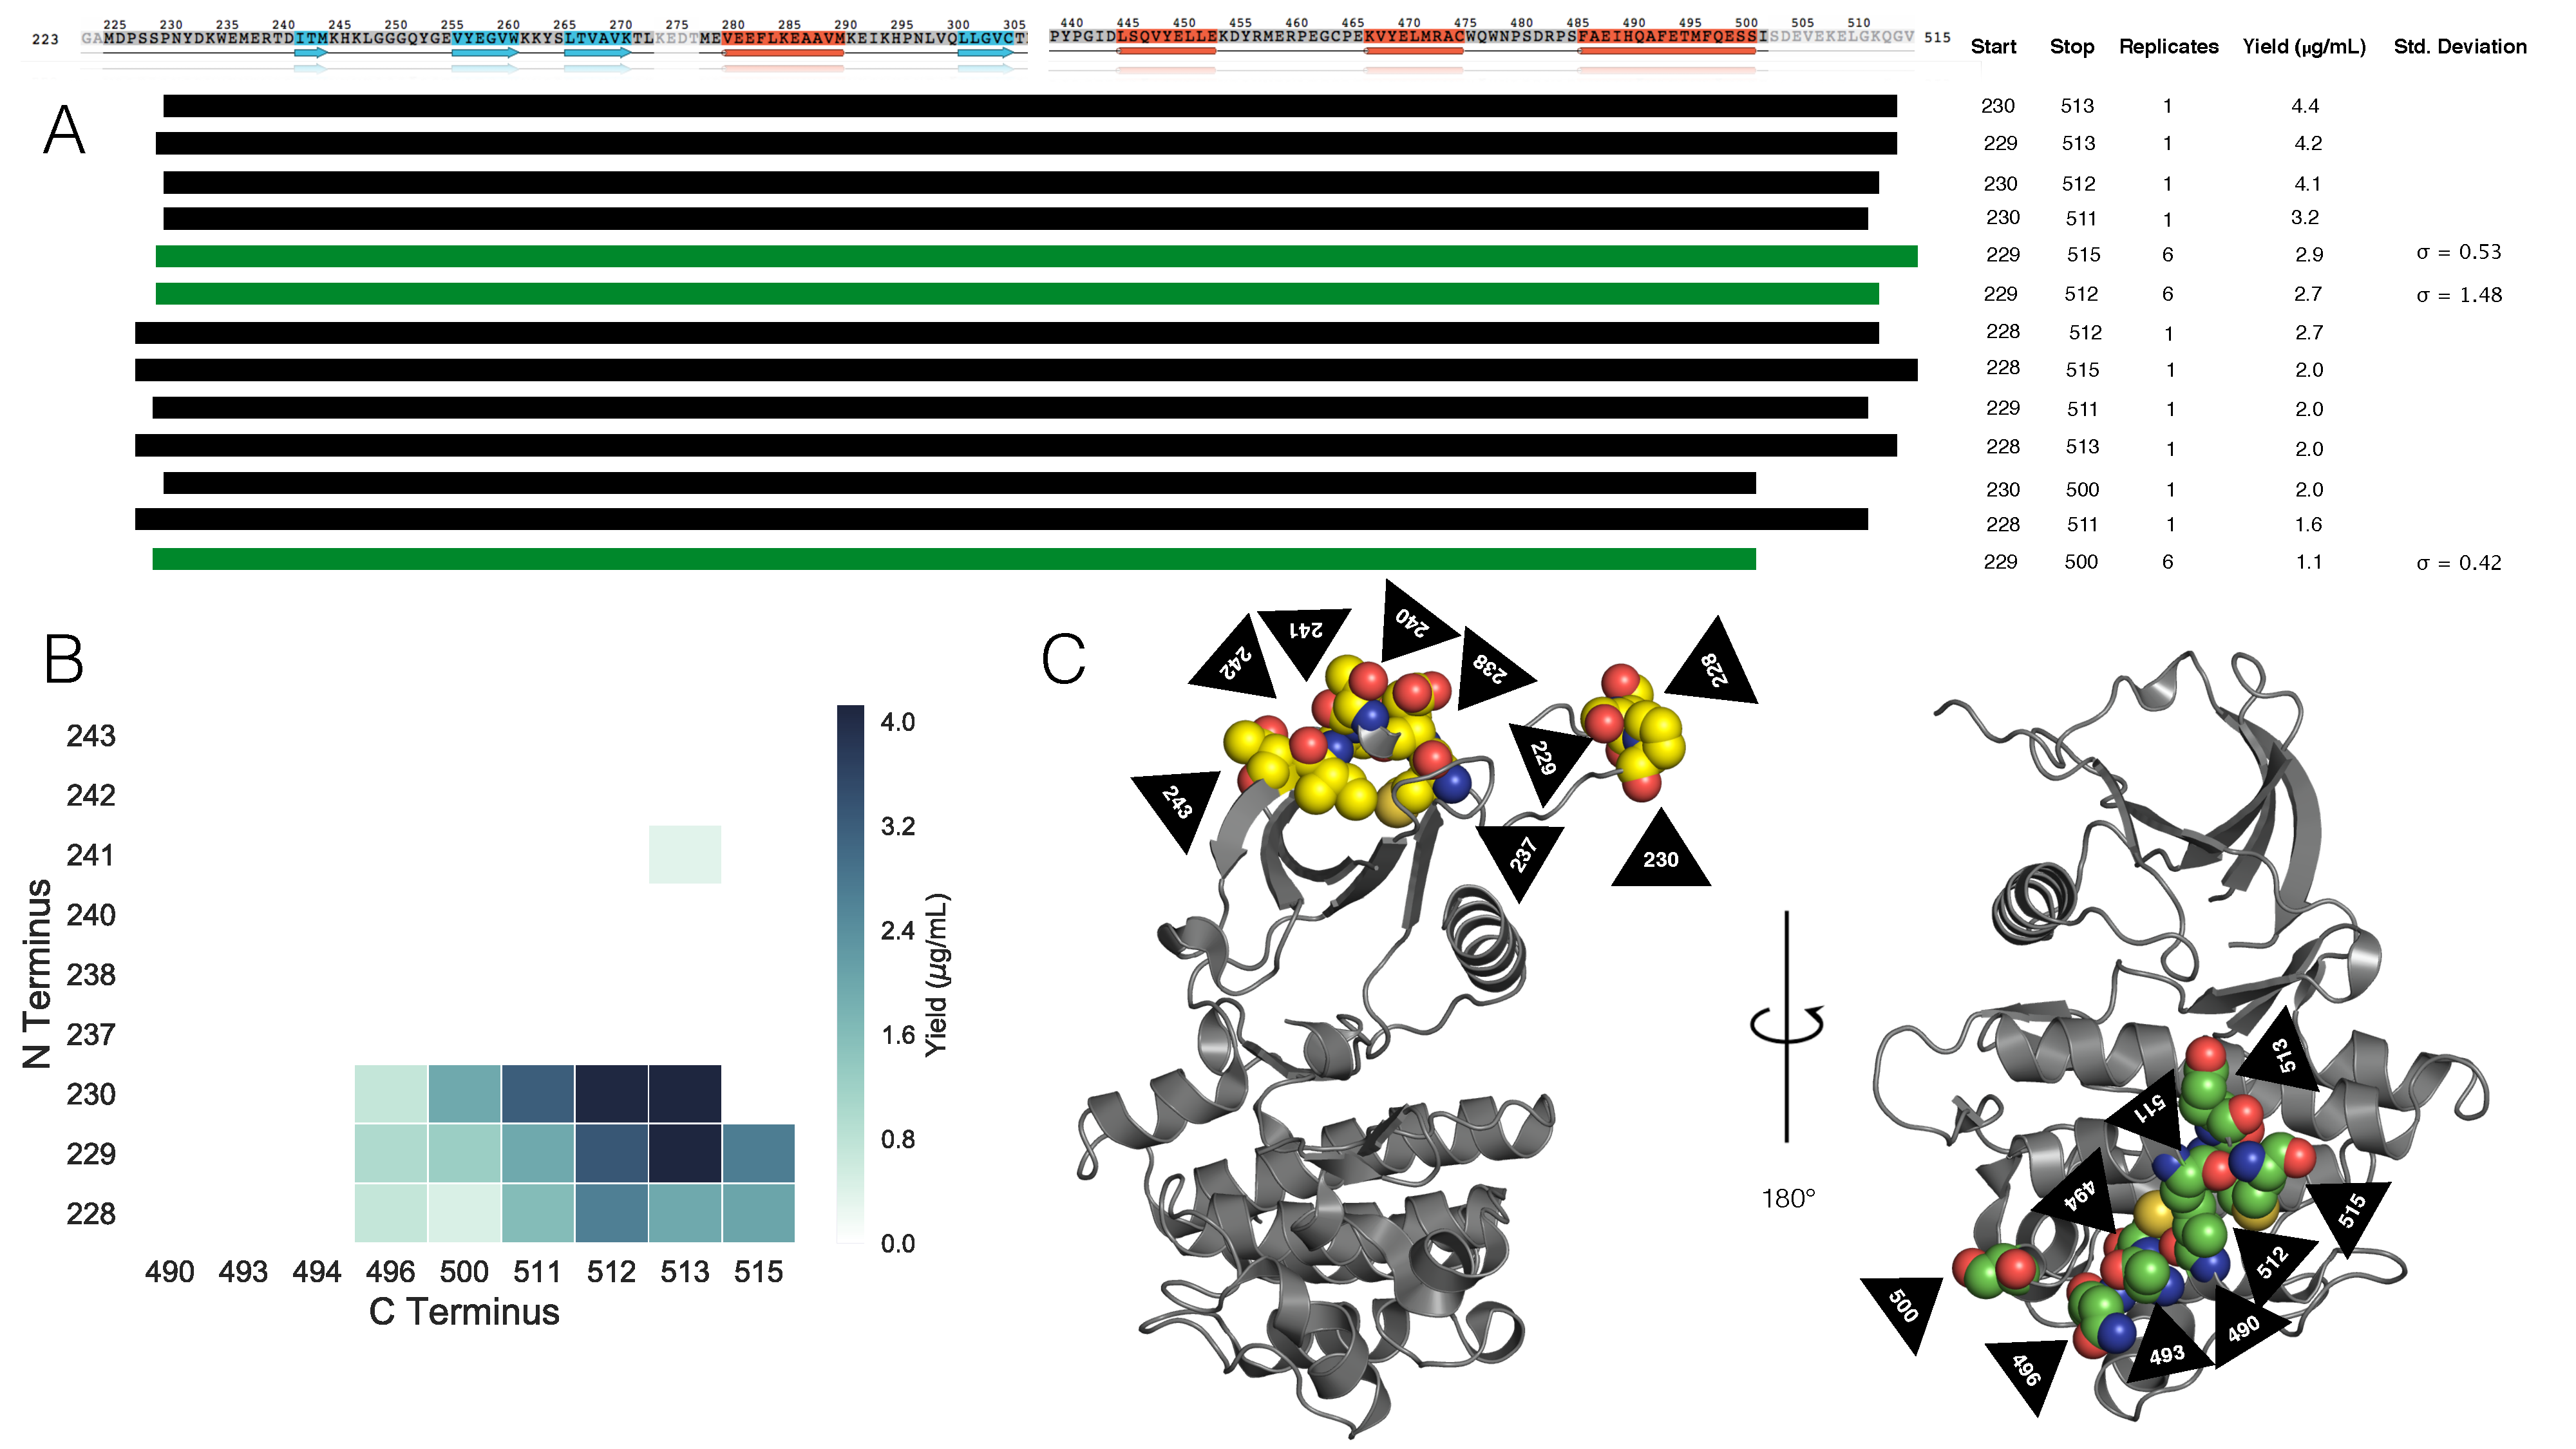
\includegraphics[width=\linewidth]{figures/abl1-construct-wholefigure.pdf}
	\caption[Abl kinase domain construct expression screen illustrates high sensitivity to construct boundaries.]{{\bf Abl kinase domain construct expression screen illustrates high sensitivity to construct boundaries.}
		({\bf A}) Abl kinase domain construct boundaries with highest expression yields. 
		Standard deviations of the yield are listed for control constructs for which six replicates were performed to give an indication of the uncertainty in experimental constructs. Secondary structure is indicated on the sequence. Beta sheets are colored blue and alpha helices are colored orange. 
		({\bf B}) Heatmap showing average yields for constructs (in $\mu$g/mL culture) with detectable expression as a function of N- and C-terminal construct boundaries.
		({\bf C}) \emph{left}: PDBID: 2E2B with the nine N-terminal construct boundary amino acids shown as yellow spheres. 
		\emph{right}: PDBID: 4XEY with the nine C-terminal construct boundary amino acids shown as green spheres. 
		Black arrows indicate residue numbers. 
	}
	\label{fig:ab1-const-fig}
	\end{figure}
\end{landscape}

\begin{landscape}
	\begin{figure}[p]
		\centering
		 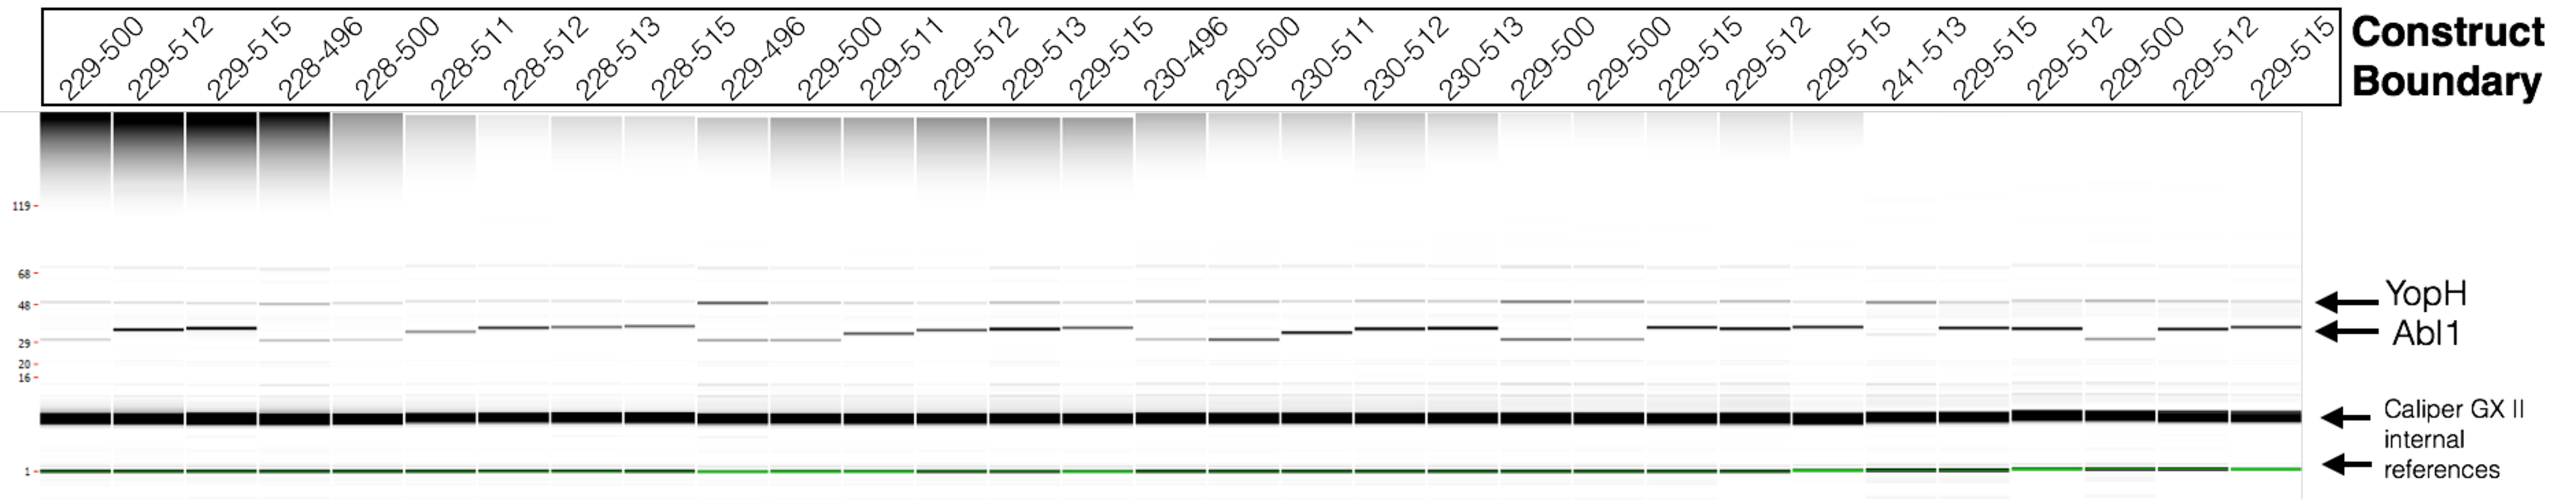
\includegraphics[width=\linewidth]{figures/abl1-construct-gel.pdf}
		\caption[Expression yields of Abl kinase domain constructs for all constructs with detectable expression.]{{\bf Expression yields of Abl kinase domain constructs for all constructs with detectable expression.}
			A synthetic gel image rendering generated from Caliper GX II microfluidic gel electrophoresis data following Ni-affinity purification and thermal denaturation for all Abl constructs with detectable expression. 
			Each well is marked with the Abl kinase domain construct residue boundaries (Uniprot canonical isoform numbering). 
			Bands for YopH164 phosphatase (50 kDA) and Abl kinsase domain constructs (28--35 kDA) are labeled. 
		}
		\label{fig:abl1_caliper_image}
	\end{figure}
\end{landscape}

\subsection{Screen of 96 kinases finds 52 with useful levels of automated \emph{E.~coli} expression}
To begin exploring which human kinase domains can achieve useful expression in \emph{E.~coli} using a simple automatable expression and purification protocol, a panel of kinase domain constructs for 96 kinases, for which bacterial expression has been previously demonstrated, was assembled using a semi-automated bioinformatics pipeline. 
Briefly, a database was built by querying Uniprot~\citep{uniprot:2017} for human protein kinase domains that were both active and not truncated. 
This query returned a set of target sequences that were then matched to their relevant PDB constructs and filtered for expression system (as determined from PDB header {\tt EXPRESSION\_SYSTEM} records), discarding kinases that did not have any PDB entries with bacterial expression. 
As a final filtering step, the kinases were compared to three purchased kinase plasmid libraries (described in Methods), discarding kinases without a match. Construct boundaries were selected from PDB constructs and the SGC plasmid library, both of which have experimental evidence for \emph{E. coli} expression, and subcloned from a plasmid in a purchased library (see Methods).
Selecting the kinases and their constructs for this expression trial in this method rested on the basis of expected success: these specific kinase constructs were bacterially expressed and purified to a degree that a crystal structure could be solved. 
While expression protocols used to produce protein for crystallographic studies are often individually tailored, we considered these kinases to have a high likelihood of expressing in our semi-automated pipeline where the \emph{same} protocol is utilized for all kinases. 
Statistics of the number of kinases obtained from the PDB mining procedure are shown in Figure~\ref{fig:kinome-expression}A. 
Surprisingly, the most highly sampled family was the CAMK family, suggesting researchers may have found this family particularly amenable to bacterial expression.
Based on the results of the previous experiment scanning Abl constructs for expression, we decided to use construct boundaries that were reported in the literature for each kinase. 
This process resulted in a set of 96 plasmid constructs distributed across kinase families (Figure~\ref{fig:kinome-expression}B). 

\begin{landscape}
	\begin{figure}[p]
		\centering
 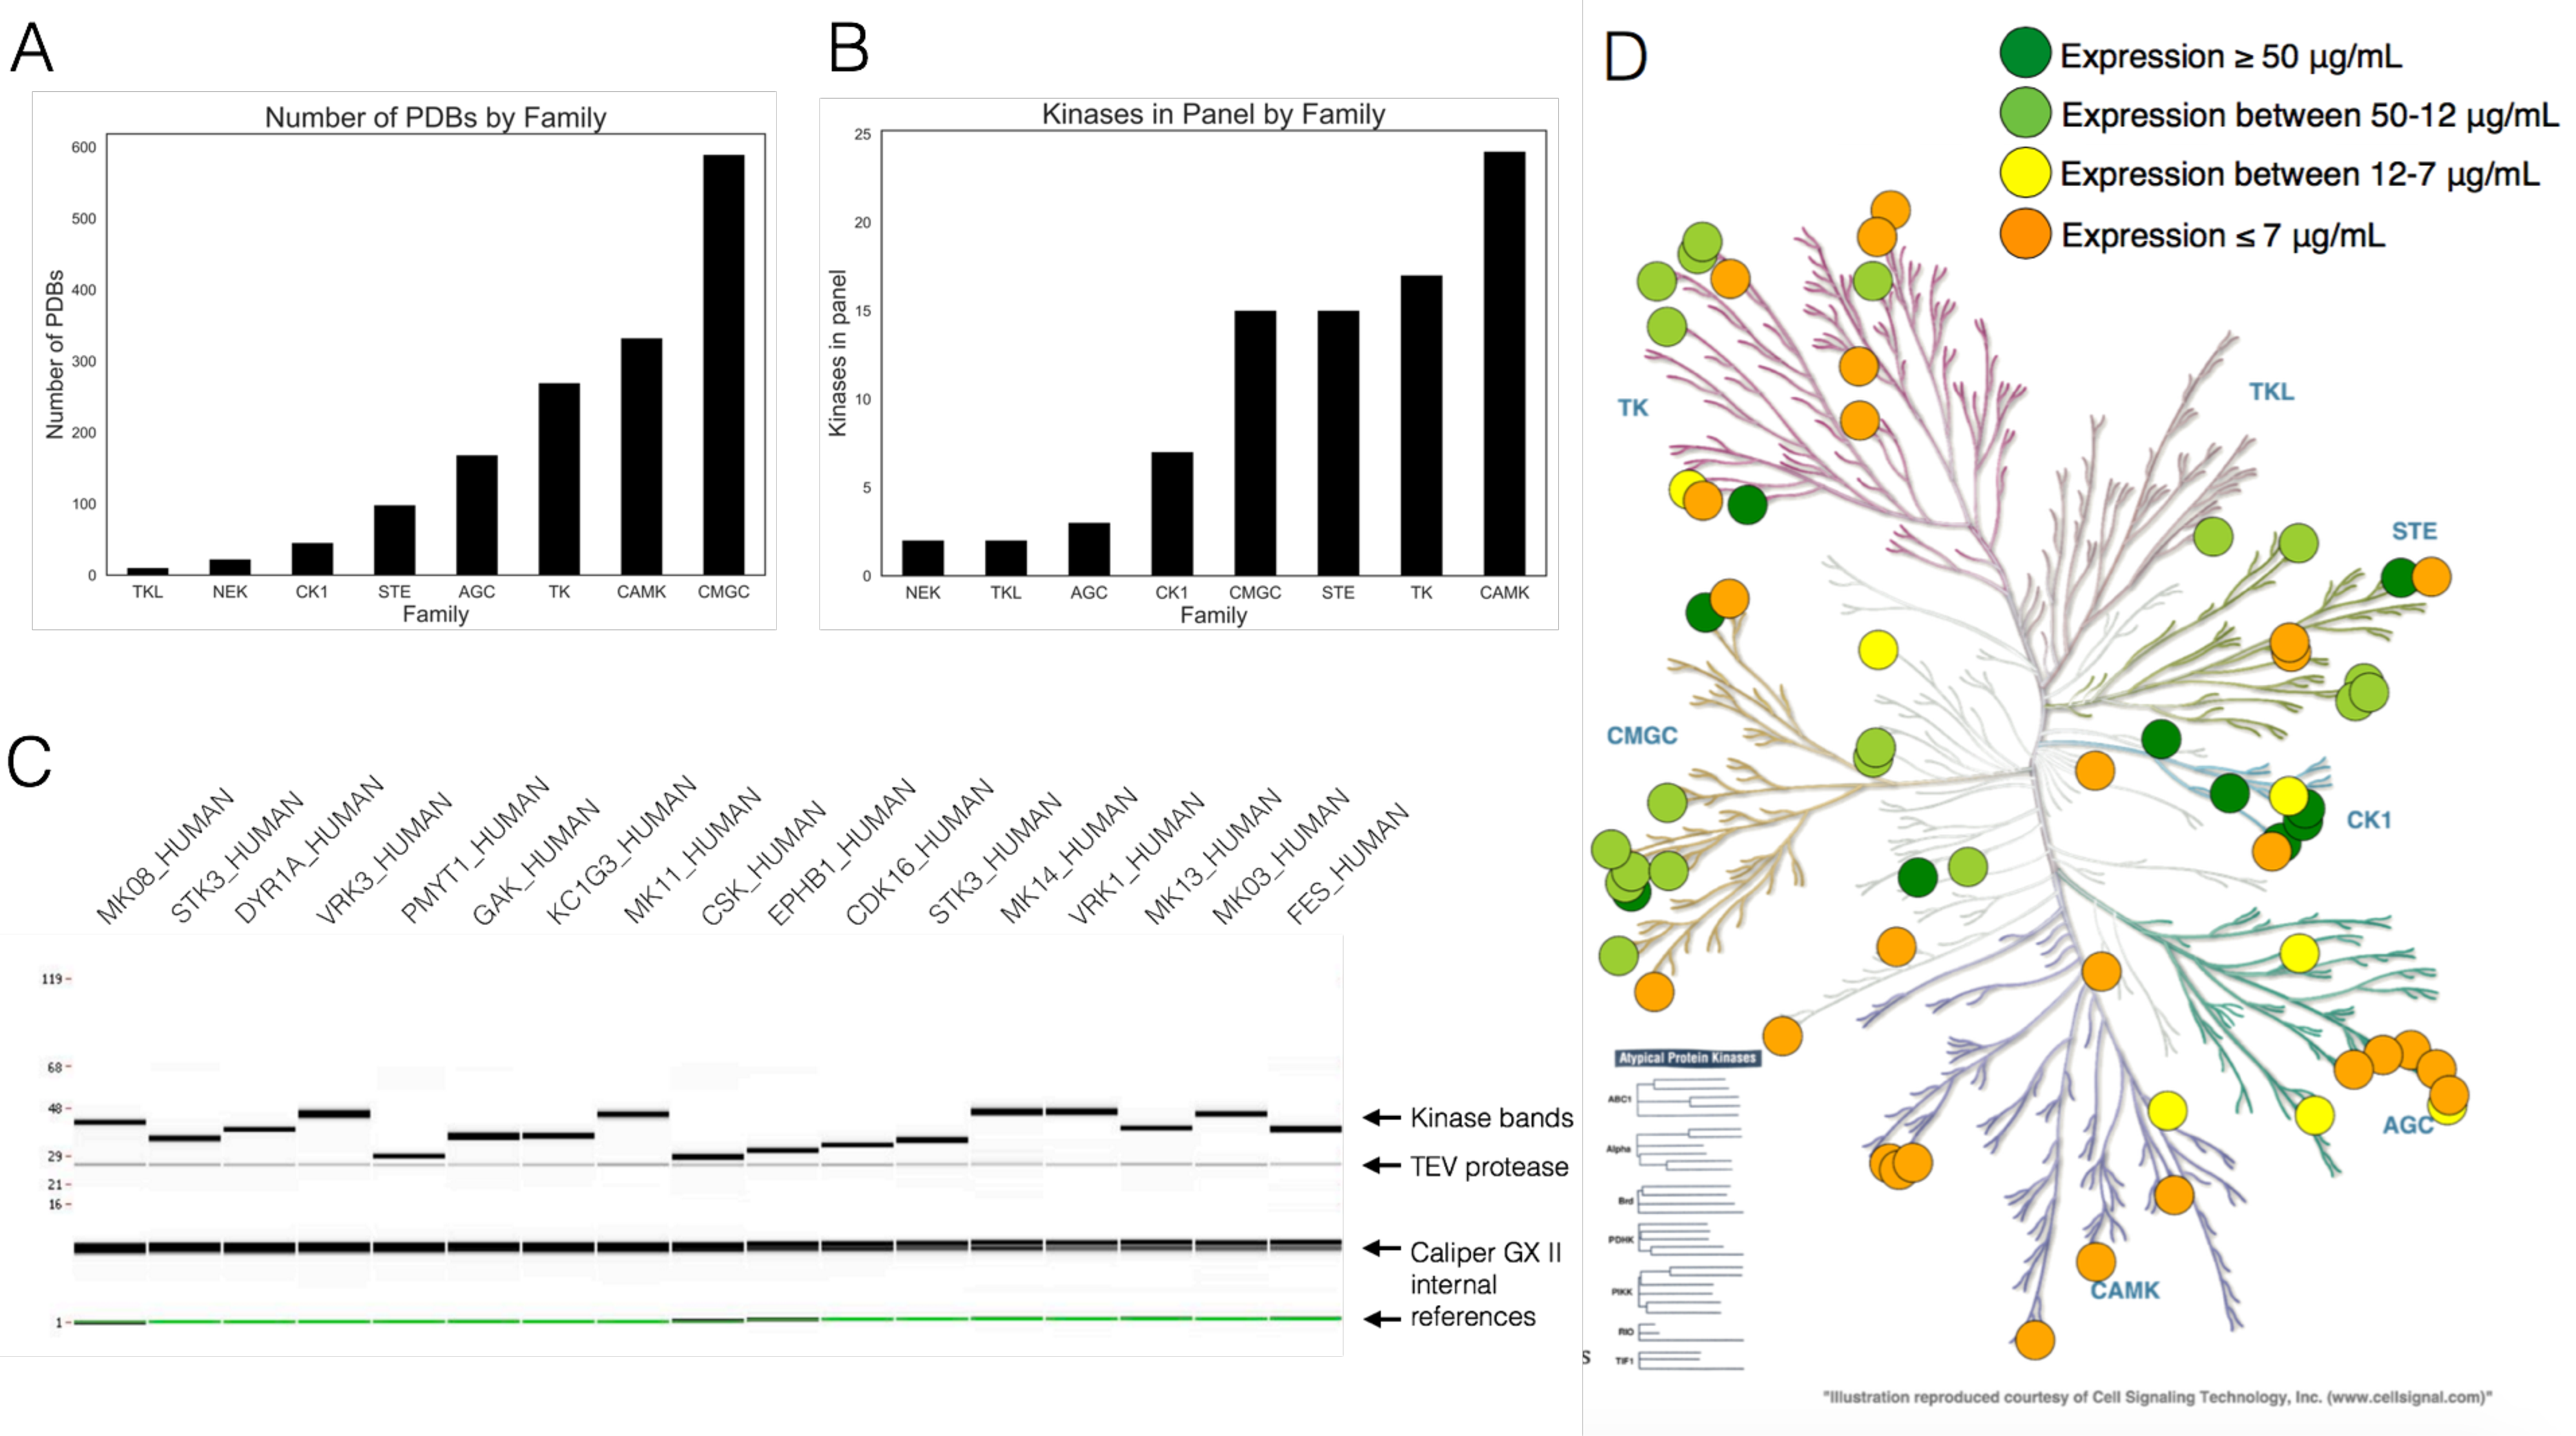
\includegraphics[width=\linewidth]{figures/96-kinase-figure}
\caption[Kinome wide search for expressible kinases.]{{\bf Kinome wide search for expressible kinases.}
	({\bf A}) The number of PDB structures per kinase family, from the database built to select kinases for expression. ({\bf B}) The distribution among familes of candidate kinases in our expression screen. ({\bf C}) Caliper GX II synthetic gel image rendering of the highest expressing kinases, quantified using microfluidic capillary electrophoresis.  ({\bf D}) Kinome distribution of expression based on our 96 kinase screen. Dark green circles represent kinases with expression above 50~$\mu$g/mL culture yield.
	Light green circles represent kinases with expression between 50 and 12~$\mu$g/mL yield.
	Yellow circles represent kinases with expression between 12 and 7~$\mu$g/mL yield.
	Orange circles represent kinases with any expression (even below 2~$\mu$g/mL) up to 7~$\mu$g/mL yield.
	Image made with KinMap: \href{http://www.kinhub.org/kinmap}{http://www.kinhub.org/kinmap}. 
}
\label{fig:kinome-expression}
\end{figure}
\end{landscape}

\definecolor{forestgreen}{RGB}{10, 67, 28}
\begin{landscape}
	\realsinglespacing
	\begin{longtable}[c]{lllll}
	\caption[Kinase domain constructs with yields $>$2 $\mu$g/mL culture for 96-kinase expression screen.]{{\bf Kinase domain constructs with yields $>$2 $\mu$g/mL culture for 96-kinase expression screen.} 
		Kinases are listed by Uniprot designation and whether they were co-expressed with Lambda or truncated YopH164 phosphatase.
		Yield (determined by Caliper GX II quantitation of the expected size band) reported in $\mu$g/mL culture, where total eluate volume was 120 $\mu$L from 900 $\mu$L bacterial culture. 
		Yields are shaded green (yield $>$ 12 $\mu$g/mL), yellow (12 $>$ yield $>$ 7 $\mu$g/mL) and orange (yield $<$ 7 $\mu$g/mL); kinase domain constructs with yields that were undetectable or $<$ 2 $\mu$g/mL are not listed.  
		$\ddag$ denotes that the second kinase domain of KS6A1\_HUMAN was expressed; all other kinases were the first or only kinase domain occurring in the ORF.
		Construct boundaries are listed in UniProt residue numbering for the UniProt canonical isoform.
		An interactive table of expression yields and corresponding constructs is available at \url{http://choderalab.org/kinome-expression}
	}	
	\label{expression_table} \\
		\toprule
		\bf{Kinase} & \bf{Construct Boundary} & \bf{Plasmid Source and ID}& \bf{Phosphatase} & \bf{Yield ($\mu$g/mL)} \\ \midrule \\
		\endfirsthead
			%
		\multicolumn{5}{c}
		{{\bf Table \thetable\ continued from previous page}} \\
		\bf{Kinase} & \bf{Construct Boundary} & \bf{Plasmid Source and ID}& \bf{Phosphatase} & \bf{Yield ($\mu$g/mL)} \\ \midrule \\
		\endhead
		%
		
		MK14\_HUMAN & 1--360& Addgene 23865&	Lambda                    & \cellcolor{forestgreen!55}\bf{70.7}                            \\
		VRK3\_HUMAN & 24--352&SGC Oxford	VRK3A-c016 & Lambda                    & \cellcolor{forestgreen!55}\bf{67.5}                            \\
		GAK\_HUMAN  & 24--359& SGC Oxford GAKA-c006 & Lambda                    & \cellcolor{forestgreen!55}\bf{64.7}                            \\
		CSK\_HUMAN  & 186--450& Addgene	23941 & YopH         & \cellcolor{forestgreen!55}\bf{62.5}                            \\
		VRK1\_HUMAN & 3--364& Addgene	23496 & Lambda                    & \cellcolor{forestgreen!55}\bf{62.3}                            \\
		KC1G3\_HUMAN & 24--351 & SGC Oxford CSNK1G3A-c002 & Lambda                    & \cellcolor{forestgreen!55}\bf{56.3}                            \\
		FES\_HUMAN  & 448--822 & Addgene 23876 & YopH         & \cellcolor{forestgreen!55}\bf{44.0}                            \\
		PMYT1\_HUMAN & 24--311& SGC Oxford	PKMYT1A-c004 & Lambda                    & \cellcolor{forestgreen!55}\bf{38.0}                            \\
		MK03\_HUMAN  & 1--379 & Addgene	23509 &Lambda                    & \cellcolor{forestgreen!55}\bf{36.4}                            \\
		STK3\_HUMAN  &16--313 & Addgene	23818 & Lambda                    & \cellcolor{forestgreen!55}\bf{34.3}                            \\
		DYR1A\_HUMAN & 24--382& SGC Oxford	DYRK1AA-c004 & Lambda                    & \cellcolor{forestgreen!55}\bf{34.1}                            \\
		KC1G1\_HUMAN & 24--331& SGC Oxford	CSNK1G1A-c013 & Lambda                    & \cellcolor{forestgreen!55}\bf{34.1}                            \\
		MK11\_HUMAN  & 24--369 & SGC Oxford	MAPK11A-c007 & Lambda                    & \cellcolor{forestgreen!55}\bf{31.7}                            \\
		MK13\_HUMAN  &1--352 & Addgene 23739&Lambda                    & \cellcolor{forestgreen!55}\bf{31.7}                            \\
		EPHB1\_HUMAN & 602--896& Addgene 23930& YopH         & \cellcolor{forestgreen!55}\bf{28.9}                            \\
		MK08\_HUMAN  & 1--363 & HIP pJP1520 HsCD00038084 & Lambda                    & \cellcolor{forestgreen!55}\bf{28.5}                            \\
		CDK16\_HUMAN &163--478 & Addgene 23754 & Lambda                    & \cellcolor{forestgreen!55}\bf{26.9}                            \\
		EPHB2\_HUMAN &604--898& HIP pJP1520 HsCD00038588 & YopH         & \cellcolor{forestgreen!55}\bf{25.1}                            \\
		PAK4\_HUMAN  &291--591 & Addgene 23713 & Lambda                    & \cellcolor{forestgreen!55}\bf{23.9}                            \\
		CDKL1\_HUMAN & 2--304& SGC Oxford CDKL1A-c024 & Lambda                    & \cellcolor{forestgreen!55}\bf{23.2}                            \\
		SRC\_HUMAN   & 254--536 & Addgene 23934 & YopH         & \cellcolor{forestgreen!55}\bf{22.0}                            \\
		STK16\_HUMAN & 24--316 & SGC Oxford STK16A-c002 & Lambda                    & \cellcolor{forestgreen!55}\bf{20.7}                            \\
		MAPK3\_HUMAN & 33--349 & Addgene 23790 & Lambda                    & \cellcolor{forestgreen!55}\bf{18.8}                            \\
		PAK6\_HUMAN  & 383--681 & Addgene 23833 & Lambda                    & \cellcolor{forestgreen!55}\bf{18.0}                            \\
		CSK22\_HUMAN & 1--334 & HIP pJP1520 HsCD00037966 & Lambda                    & \cellcolor{forestgreen!55}\bf{17.9}                            \\
		MERTK\_HUMAN & 570--864 & Addgene 23900 & YopH         & \cellcolor{forestgreen!55}\bf{16.8}                            \\
		PAK7\_HUMAN  & 24--318 & SGC Oxford PAK5A-c011 & Lambda                    & \cellcolor{forestgreen!55}\bf{14.7}                            \\
		CSK21\_HUMAN & 1--335 & Addgene 23678 & Lambda                    & \cellcolor{forestgreen!55}\bf{14.5}                            \\
		EPHA3\_HUMAN & 606--947 & Addgene 23911 & YopH         & \cellcolor{forestgreen!55}\bf{14.1}                            \\
		BMPR2\_HUMAN & 1--329 & SGC Oxford BMPR2A-c019 & Lambda                    & \cellcolor{forestgreen!55}\bf{14.1}                            \\
		M3K5\_HUMAN  & 659--951 & HIP pJP1520 HsCD00038752 & Lambda                    & \cellcolor{forestgreen!55}\bf{14.0}                            \\
		KCC2G\_HUMAN & 24--334 & SGC Oxford CAMK2GA-c006 & Lambda                    & \cellcolor{forestgreen!55}\bf{13.3}                            \\
		E2AK2\_HUMAN & 254--551 & HIP pJP1520 HsCD00038350 & Lambda                    & \cellcolor{yellow!55}\bf{11.6}                            \\
		MK01\_HUMAN  & 1--360 & HIP pJP1520 HsCD00038281 & Lambda                    & \cellcolor{yellow!55}\bf{11.2}                            \\
		CSKP\_HUMAN  & 1--340 & HIP pJP1520 HsCD00038384 & Lambda                    & \cellcolor{yellow!55}\bf{10.1}                            \\
		CHK2\_HUMAN  & 210--531 & Addgene 23843 & Lambda                    & \cellcolor{yellow!55}\bf{8.1}                             \\
		KC1G2\_HUMAN & 4--312 & SGC Oxford CSNK1G2A-c002 & Lambda                    & \cellcolor{yellow!55}\bf{7.6}                             \\
		DMPK\_HUMAN  &2 4--433 & SGC Oxford DMPK1A-c026 & Lambda                    & \cellcolor{yellow!55}\bf{7.6}                             \\
		KCC2B\_HUMAN & 11--303 & Addgene 23820 & Lambda                    & \cellcolor{yellow!55}\bf{7.1}                             \\
		FGFR1\_HUMAN & 456--763 & Addgene 23922 & YopH         & \cellcolor{orange!55}\bf{6.1}                             \\
		KS6A1\_HUMAN$^\ddag$ &413--735 & SGC Oxford RPS6KA1A-c036 &   Lambda                    & \cellcolor{orange!55}\bf{5.7}                             \\
		DAPK3\_HUMAN & 9--289 & Addgene 23436 &  Lambda                    & \cellcolor{orange!55}\bf{4.0}                             \\
		STK10\_HUMAN & 18--317 & HIP pJP1520 HsCD00038077 &  Lambda                    & \cellcolor{orange!55}\bf{3.7}                             \\
		KC1D\_HUMAN  & 1--294 & Addgene 23796 & Lambda                    & \cellcolor{orange!55}\bf{3.7}                             \\
		KC1E\_HUMAN  & 1--294 & Addgene 23797 & Lambda                    & \cellcolor{orange!55}\bf{3.5}                             \\
		NEK1\_HUMAN  & 23--350 & SGC Oxford NEK1A-c011 & Lambda                    & \cellcolor{orange!55}\bf{3.3}                             \\
		CDK2\_HUMAN  & 1--297 & Addgene 23777 & Lambda                    & \cellcolor{orange!55}\bf{3.1}                             \\
		ABL1\_HUMAN  & 229--512 & HIP pJP1520 HsCD00038619 & YopH         & \cellcolor{orange!55}\bf{2.5}                             \\
		DAPK1\_HUMAN & 2--285 & HIP pJP1520 HsCD00038376 & Lambda                    & \cellcolor{orange!55}\bf{2.4}                             \\
		DYRK2\_HUMAN & 23--417 & SGC Oxford DYRK2A-c023 & Lambda                    & \cellcolor{orange!55}\bf{2.4}                             \\
		HASP\_HUMAN  & 24--357 & SGC Oxford GSG2A-c009 &  Lambda                    & \cellcolor{orange!55}\bf{2.3}                             \\
		FGFR3\_HUMAN & 449--759	& Addgene 23933 & YopH         & \cellcolor{orange!55}\bf{2.3}                             \\
		\bottomrule
\end{longtable}
\end{landscape}

From these constructs, a set of 96 His10-TEV N-terminally tagged kinase domain constructs were generated, coexpressed with a phosphatase in \emph{E.~coli}, purified via nickel bead pulldown, and quantified using microfluidic gel electrophoresis.
The 96 kinases were coexpressed with either Lambda phosphatase (for Ser/Thr kinases) or a truncated form of YopH phosphatase\footnote{Yoph164 phosphatase, engineered to minimize intrinsic affinity for nickel purification resin by the QB3 MacroLab based on parent plasmid pCDFDuet1-YOPH, a gift from the Kuriyan Lab.} (for Tyr kinases). 

Instead of eluting with imidazole, purified kinase was cleaved off nickel beads by the addition of 10\% TEV protease to minimize phosphatase contamination in the resulting eluate, allowing us to assess whether resulting yields would be sufficient (and sufficiently free of phosphatase) to permit activity assays.
While the initial panel of 96 kinases was well-distributed among kinase families (Figure~\ref{fig:kinome-expression}B), the most highly expressing kinases (yield of more than 12~$\mu$g kinase/mL culture) were not evenly distributed (Figure~\ref{fig:kinome-expression}D). While many of the kinases chosen from the CMGC and CK1 families expressed well in our panel, nearly all of the kinases from the CAMK and AGC family express below 12~$\mu$g kinase/mL (Figure~\ref{fig:kinome-expression}D).   
52 kinases demonstrated a useful level of soluble protein expression, here defined as greater than 2 $\mu$g/mL, na\"{i}vely expected to scale up to better than 2 mg/L culture (Table~\ref{expression_table}). 
Some kinases (shaded green in Table~\ref{expression_table}) demonstrated very high levels of expression, while others (shaded orange in Table~\ref{expression_table}) would likely benefit from further rounds of construct boundary optimization or solubility tags to boost soluble expression. 
The 17 most highly expressing kinases showed relatively high purity after elution, though we note that eluting via TEV site cleavage results in a quantity of TEV protease in the eluate (Figure~\ref{fig:kinome-expression}C), but does not cause the elution of the His-tagged phosphatases which would hinder the ability to perform kinase activity assays. 
Further optimization of elution conditions may be required for optimizing kinase recovery via TEV cleavage~\citep{Puhl:2009gg,Nallamsetty:2004cp,Sun:2012bh}.

Constructs with expression yields above 2 $\mu$g/mL have been made available via {\bf Addgene}:
\url{https://www.addgene.org/kits/chodera-kinase-domains}

\subsection{High-expressing kinases are folded with a well-formed ATP binding site}

To determine whether the expressed kinases were properly folded, we performed both a fluorescence-based thermostability assay (Figure~\ref{fig:thermofluor}) as well as a fluorescent ATP-competitive ligand binding measurement to quantify whether the ATP binding site was well-formed (Figure~\ref{fig:binding}). 

\begin{landscape}
	\begin{figure}[p]
		\centering
		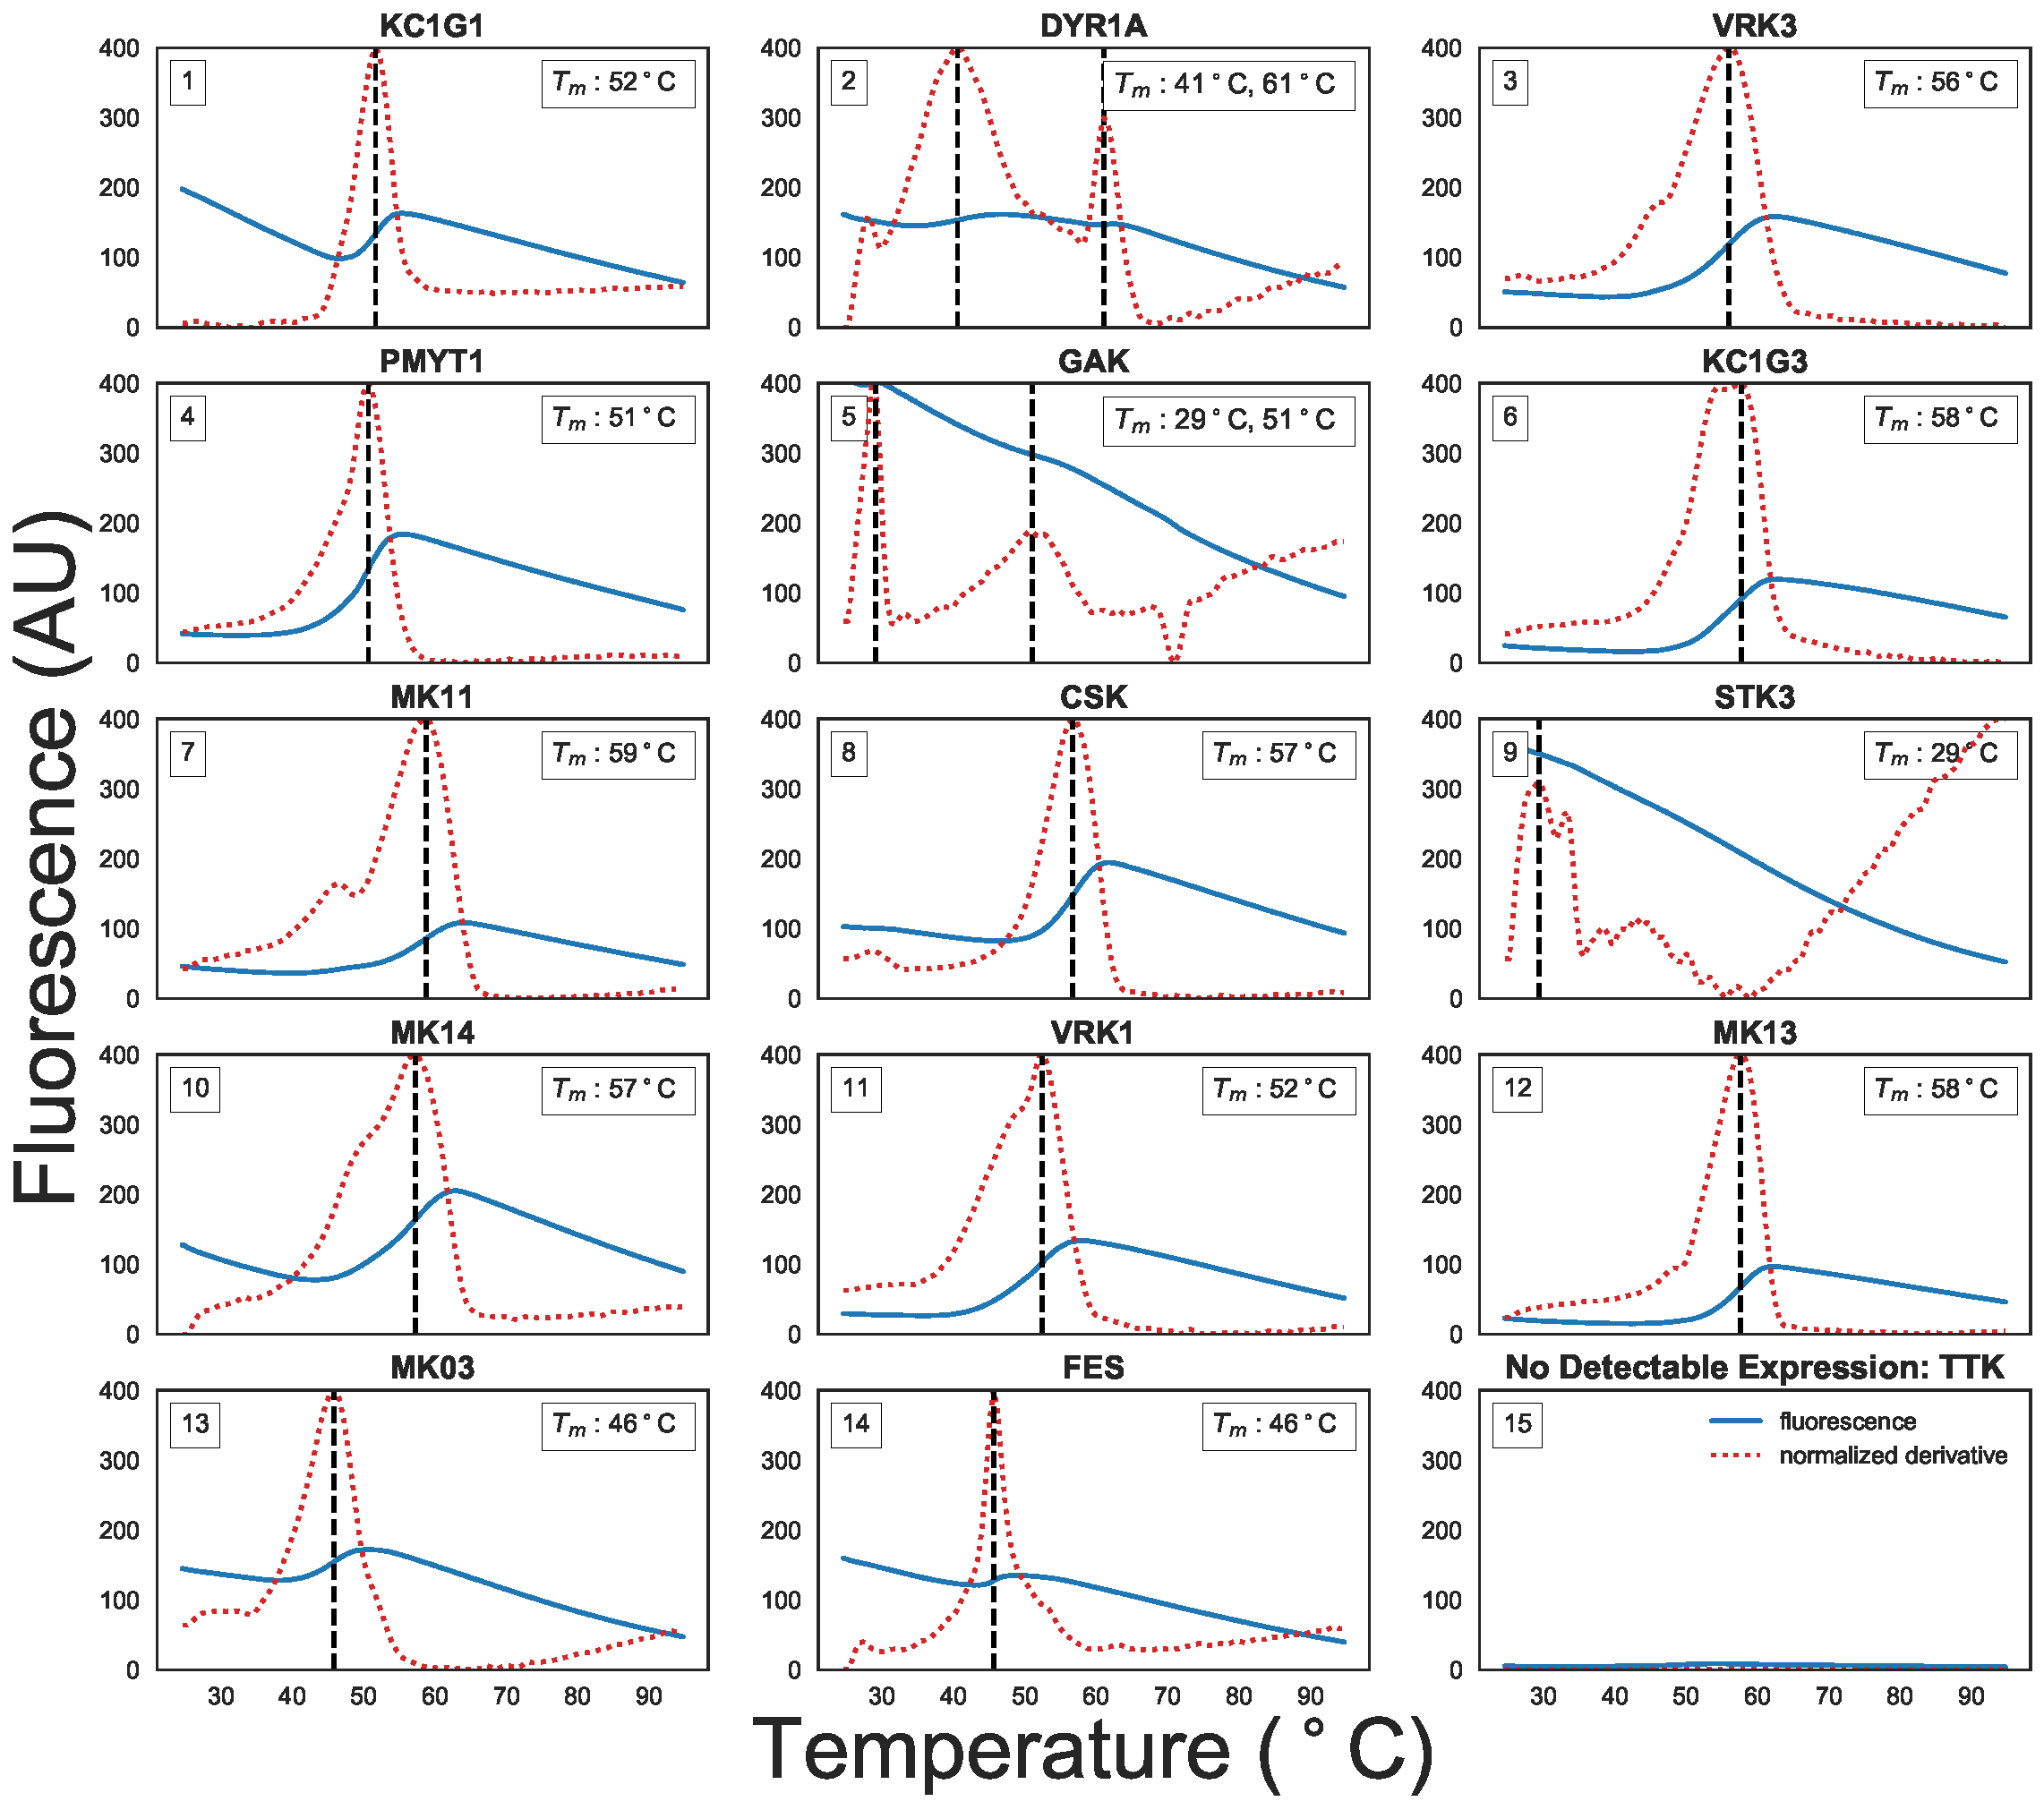
\includegraphics[width=0.6\linewidth]{figures/bothplates_dualaxis_tm}
 \caption[ Fluorescence-based thermostability assay demonstrates many high-expressing kinases are well-folded.]{{\bf Fluorescence-based thermostability assay demonstrates many high-expressing kinases are well-folded.}
	A fluorescence-based thermostability assay was performed on the 14 kinases shown to express above a minimum 0.24~mg/mL concentration after elution. 
	SYPRO Orange fluorescence (solid blue line) was measured at 580~nm (half bandwidth 20~nm) after excitation at 465~nm (half bandwith 25~nm) as as the temperature was ramped from (x-axis) in Nickel Buffer A (25~mM HEPES pH~7.5, 5\% glycerol, 400~mM NaCl, 20~mM imidazole, 1~mM BME). The temperature was held at 25$^{\circ}$C for 15~sec before ramping up to 95$^{\circ}$C with a ramp rate of 0.06$^{\circ}$C/s. 
	The unfolding temperature $T_m$ (black dashed line and insert) was determined from the maxima of the normalized first derivative of fluorescence (red dashed line). 
	Fluorescence emission at 580~nm is shown on the left y-axis.   
	To control for signals resulting from TEV protease contamination present at 0.01--0.03~mg/mL, TTK, a kinase with no detectable expression in our panel as determined via Caliper GX II quantitation was in included (panel 15). 
	%While no significant peak is observed for STK3 above room temperature, an ATP-competitive ligand-binding assay (Figure~\ref{fig:binding}) suggests this kinase is still well-folded.
}
\label{fig:thermofluor}
	\end{figure}
\end{landscape}

\subsection{Fluorescence-based thermostability assay}

A fluorescence-based thermostability assay was performed with the hydrophobic dye SYPRO Orange to determine whether a strong two-state unfolding signal could be observed (see Methods). 
Also referred to as \emph{thermofluor} or \emph{differential scanning fluorimetry (DSF)}, as the temperature is slowly increased, unfolded proteins will expose hydrophobic patches that SYRPO orange will bind to, causing an increase in fluorescence~\citep{Lo:2004gy,Ericsson:2006dx,Matulis:2005dq}.
While the fluorescence of solvated SYPRO Orange is temperature-dependent, clear unfolding temperatures ($T_m$) can often be identified from peaks in the first derivative of the observed fluorescence signal.
Figure~\ref{fig:thermofluor} shows the fluorescence (blue line), the absolute value of its derivative (red dashed line), and the unfolding temperature determined from the maximum absolute derivative ($T_m$) for the the 14 kinases that were eluted to concentrations above 0.24~mg/mL eluate, which was determined to be the minimum concentration required for optimal resolution of melting curves upon dilution to 10~$\mu$L. Because TEV-eluted kinase was used directly in this assay, TEV protease contaminant varies from 0.01--0.03 mg/mL in the resulting assay mix. The selected minimum concentration ensured that the kinase was roughly an order of magnitude higher concentration than the contaminating TEV. 

Most of the kinases assayed had strong peaks above room temperature, suggesting that they are well-folded in the elution buffer (25~mM HEPES pH~7.5, 5\% glycerol, 400~mM NaCl, 20~mM imidazole, 1~mM BME) at room temperature. 
Some kinases, such as a DYR1A and GAK (Figure~\ref{fig:thermofluor}, panels 6 and 9), had two shallow inflection points in SYPRO fluorescence as a function of temperature. 
While STK3 does not have a strong peak above room temperature, titration with an ATP-competitive inhibitor suggests this kinase either has a well-formed ATP binding site or folding can be induced by ligand binding (Figure~\ref{fig:binding}, panel~10). 
As a control, a sample with no detectable kinase expression (TTK from our expression panel) was assayed (Figure~\ref{fig:thermofluor}, panel~9), which showed nearly no fluorescence signal. 

\subsection{ATP-competitive inhibitor binding fluorescence assay}
To determine whether expressed kinases had well-folded ATP binding sites, we probed their ability to bind an ATP-competitive inhibitor.
While a pan-kinase inhibitor such as staurosporine could be used as a fluorescent probe~\citep{Iyer:2008is}, the ATP-competitive inhibitor bosutinib shows a much stronger increase in fluorescence around 450--480~nm when bound to kinases with well-folded ATP binding sites~\cite{levinson-boxer:plos-one:2012:bosutinib,Levinson:2014gi}. 
While excitation at 350~nm can be used, excitation at 280~nm results in lower background, potentially due to fluorescent energy transfer between kinase and ligand.
Despite the weak affinity of bosutinib for many kinases, its aqueous solubility is sufficient to provide a quantitative assessment of ATP-competitive binding to many kinases at sufficiently high concentrations to function as a useful probe~\cite{levinson-boxer:plos-one:2012:bosutinib,Levinson:2014gi}.

Here, we utilized this approach as a \emph{qualitative} probe for ATP-competitive ligand binding, due to uncertainty in the ligand concentration caused by significant evaporation over the course of the sequential titration experiment (see Methods section for a more in depth discussion). 
33 of the kinases in our expression panel had sufficient yields to prepare 100~$\mu$L of 0.5~$\mu$M kinase assay solutions, and were assessed for binding to bosutinib (Figure~\ref{fig:binding}, panels 1-33), with a concentration-dependent increase in fluorescence signal (colored spectra) over the baseline ligand fluorescence titrated into buffer (gray spectra) providing evidence of a well-formed ATP binding site. 
Six of the lowest expression kinase constructs (Figure~\ref{fig:binding}, panels 39-44) were prepared by diluted 20~$\mu$L to a reaction volume of 100~$\mu$L and assessed for bosutinib binding. Unexpectedly, these kinases also showed evidence of binding, suggesting this assay is able to detect a well-formed ATP binding site even for protein concentrations less than 0.5~$\mu$M. 
To demonstrate that unfolded kinases do not demonstrate this increase in fluorescence over ligand-only baseline, thermally denatured MK14 was included as a control next to folded MK14 from a large-scale expression prep (Figure~\ref{fig:binding}, panels 37--38), with thermally denatured MK14 exhibiting little difference from titrating ligand into buffer alone. 

\begin{landscape}
	\begin{figure}[p]
		\centering
		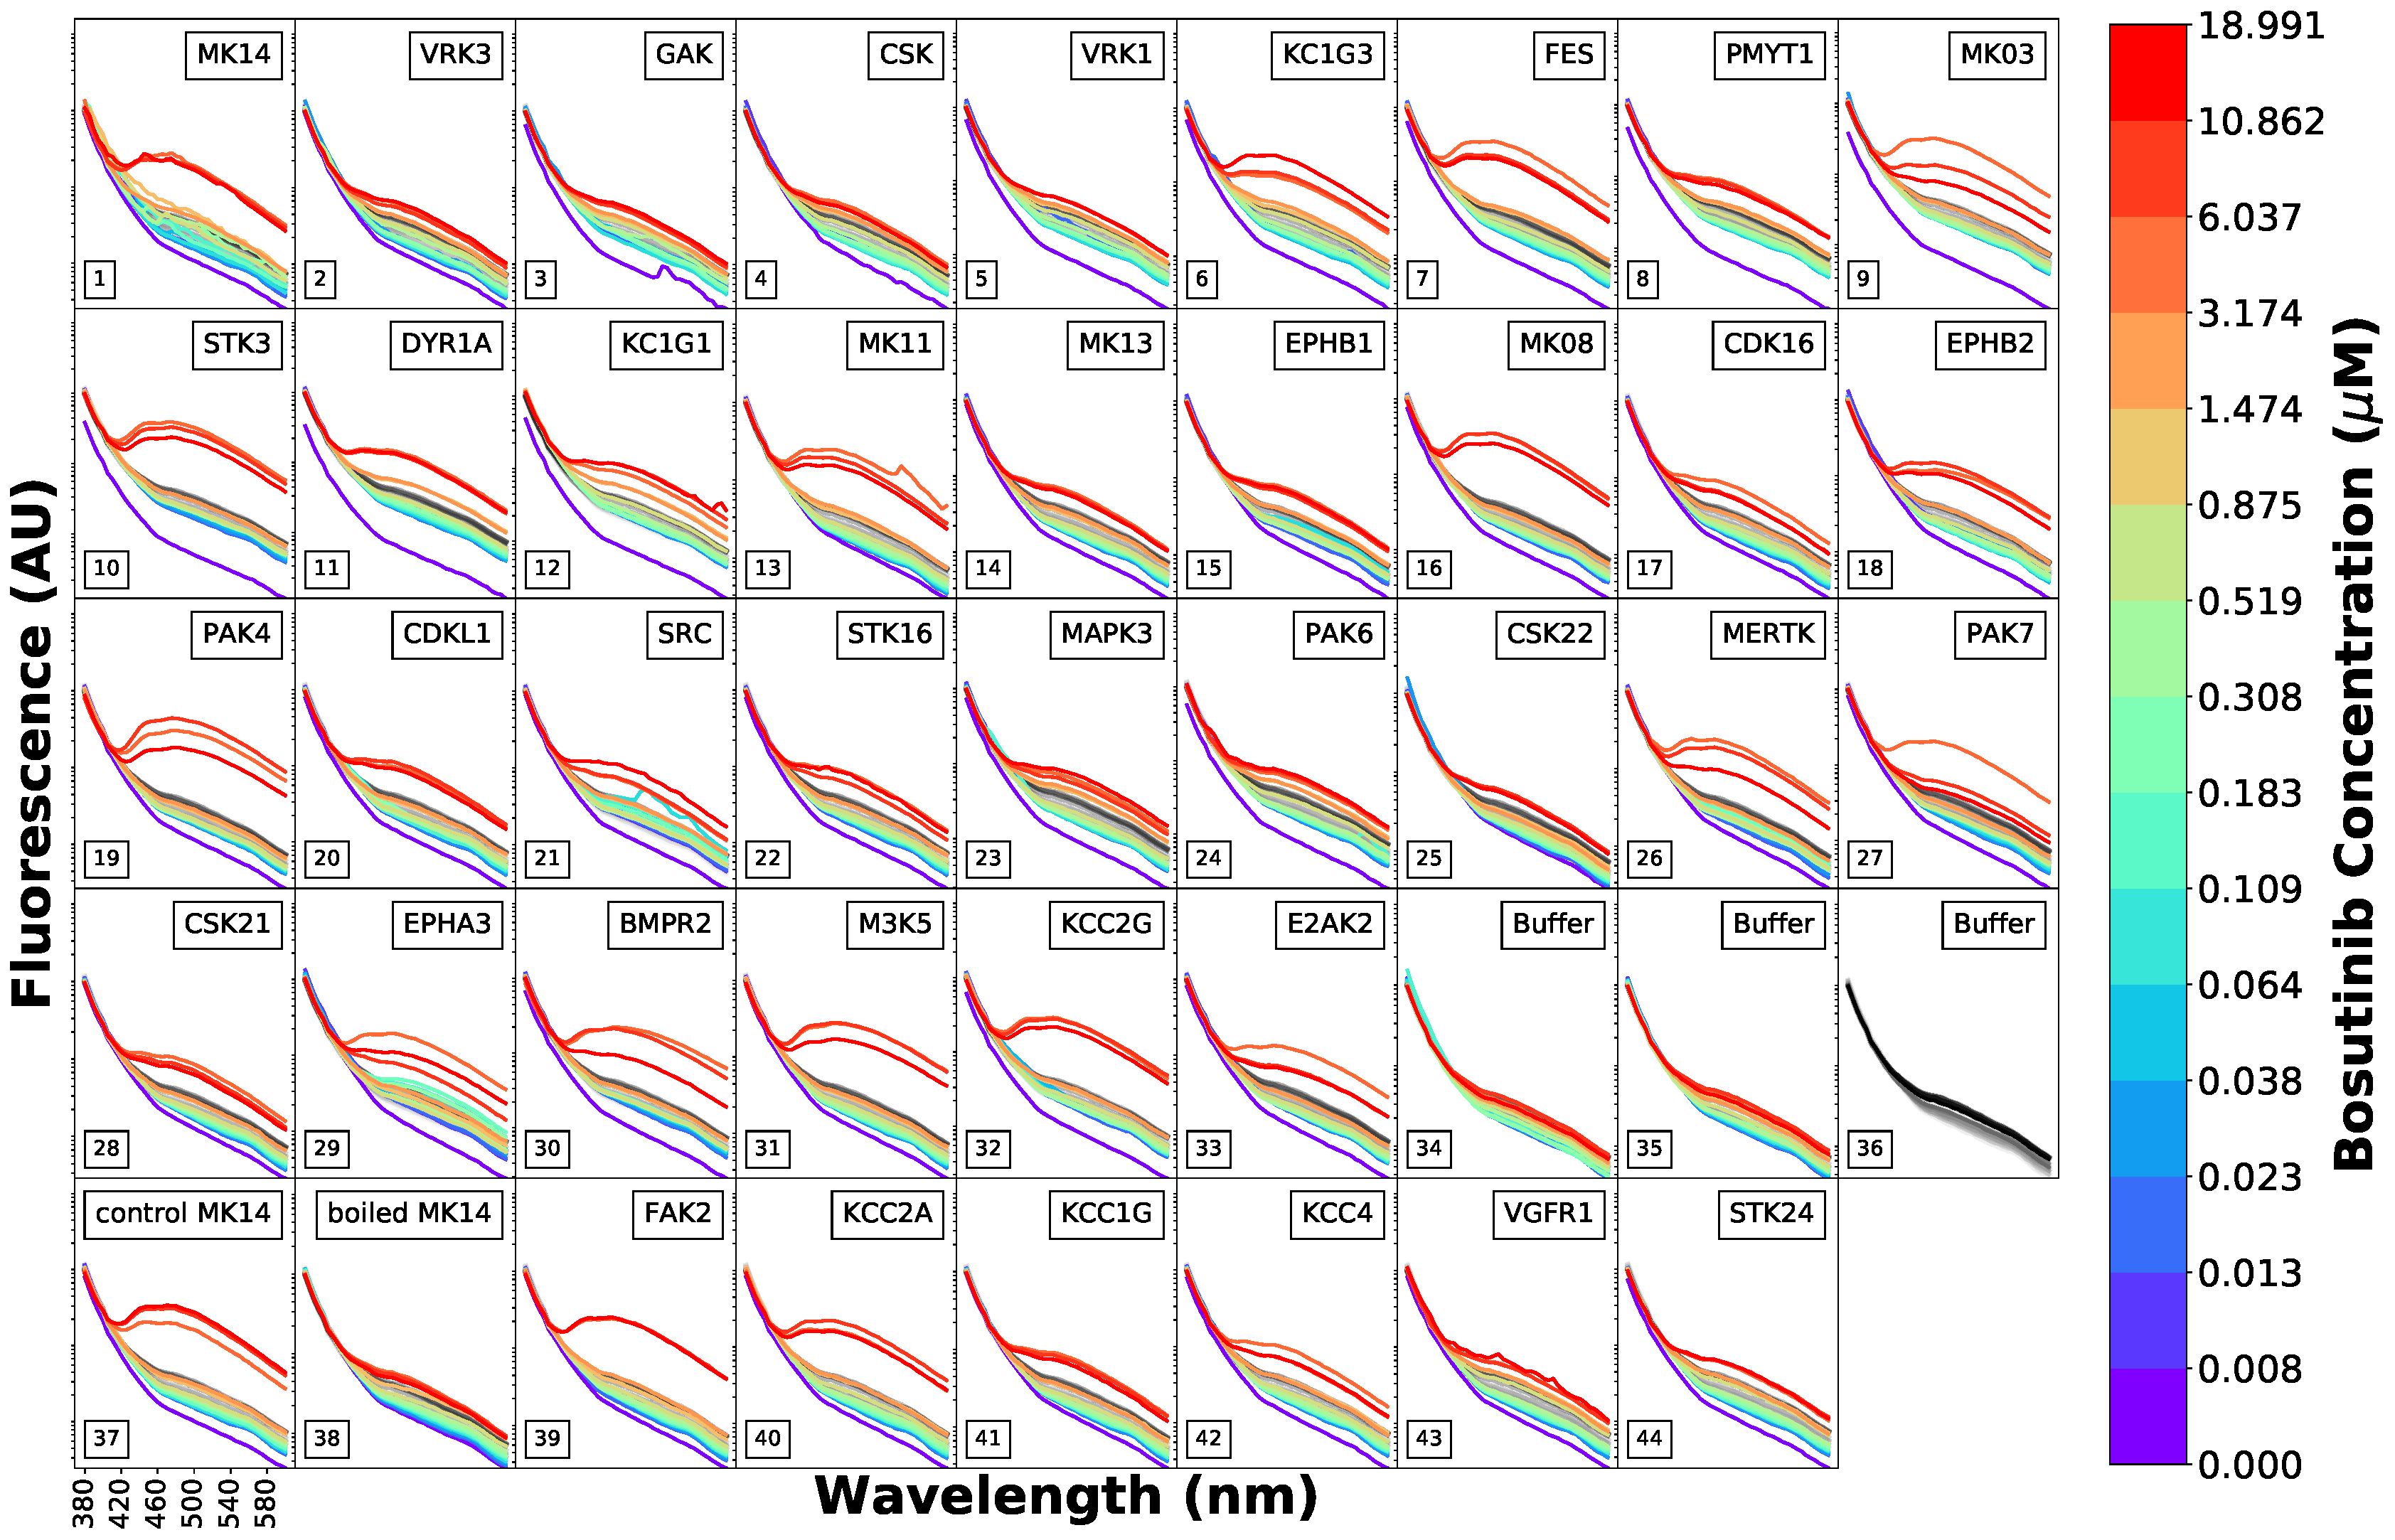
\includegraphics[width=0.6\linewidth]{figures/bos_spectra_45_logy}
		 \caption[Fluorescence emission spectra as a function of the fluorescent ATP-competitive kinase inhibitor bosutinib demonstrates the presence of a well-formed ATP binding pocket.]{{\bf Fluorescence emission spectra as a function of the fluorescent ATP-competitive kinase inhibitor bosutinib demonstrates the presence of a well-formed ATP binding pocket.}
			The ATP-competitive inhibitor bosutinib shows a strong increase in fluorescence centered around 450~nm when bound to kinases with well-folded ATP binding sites upon excitation at 280~nm~\cite{levinson-boxer:plos-one:2012:bosutinib}. 
			To assess whether the kinases from the high-throughput expression screen were well-folded, bosutinib was titrated in a 15-concentration series geometrically spanning 0.008~$\mu$M to 18.99~$\mu$M (colored lines, higher concentrations are shown in warmer colors) in 15 increments for 39 expressing kinases with protein concentration adjusted to $\sim$0.5~$\mu$M in 100~$\mu$L assay volume. 
			Eluted TEV protease contaminant varies from 0.01--0.03 mg/mL in the assay volumes.
			The control MK14 and boiled MK14 (boiled for 10~min at 95$^{\circ}$C) were produced in a large scale expression from the same plasmid as used in the high-throughput expression protocol and they were included as positive and negative controls for bosutinib binding to ATP binding pocket.
			Fluorescence emission spectra (y-axis, bandwidth 20~nm) were measured from 370~nm to 600~nm (x-axis) for excitation at 280~nm (bandwidth 10~nm). 
			For reference, the fluorescence of bosutinib titrated into buffer titration (panel 36) is shown in grayscale in each panel. 
			Significant increases in fluorescence signal above baseline qualitatively indicate the presence of a well-formed ATP binding site. 
		}
		\label{fig:binding}
	\end{figure}
\end{landscape}

\subsection{Expressing clinically-derived Src and Abl mutants}
Next-generation sequencing has enabled generation of massive datasets rich with missense alterations in kinases observed directly in the clinic~\citep{Varghese:2014jw,Zehir:2017ib,Garraway:2013kn}, and has been particularly transformative in the field of oncology. 
To determine how well our human kinase domain panel supports the automated expression of clinically-identified missense mutants for biophysical, biochemical, and structural characterization, we attempted to express 96 missense mutations mined from sequencing studies of cancer patients. 
The mutations were gathered using cBioPortal~\citep{cBioPortal} from publicly available sources and a large clinical tumor sequencing dataset from the Memorial Sloan Kettering Cancer Center~\citep{Zehir:2017ib} sequenced in the MSK-IMPACT panel~\citep{msk-impact}. 

	

\begin{landscape}
	\realsinglespacing
	\begin{ThreePartTable}
		\begin{TableNotes}
			\footnotesize
			\item [a]  Uniprot amino acid sequence numbering of primary isoform
			\item [b] MutationAssesor Score~\citep{reva_determinants_2007,doi:10.1093/nar/gkr407}, which predicts functional impact via conservation 
			\end{TableNotes}
	\begin{longtable}[c]{lllll}
	\caption[Expression yields for engineered clinical missense mutants of Abl kinase domains with yields $>$ 2~$\mu$g/mL culture.]{{\bf Expression yields for engineered clinical missense mutants of Abl kinase domains with yields $>$ 2~$\mu$g/mL culture.} 
		Abl kinase domain constructs with engineered clinical mutations with expression yields $>$2~$\mu$g/mL culture are listed, sorted by yield. 
		Yield  was determined by Caliper GX II quantitation of the expected size band and reported in $\mu$g/mL culture, where total eluate volume was 80~$\mu$L purified from 900~$\mu$L bacterial culture.
		Wild-type (WT) controls for both Src and Abl (here, a single well for each) are shown as the first entry for each gene. 
	}
	\label{mut-expression_table_abl}\\
			\toprule
			\bf{Abl1 (229--512)} & \bf{Mutation}\tnote{a} & \bf{Functional Impact Score}\tnote{b} & \bf{yield ($\mu$g/mL)} & \bf{\% of WT expression} \\  \midrule \\
			\endfirsthead
			%
			\multicolumn{5}{c}%
		{{\bf Table \thetable\ continued from previous page}} \\
			\toprule
		\bf{Abl1 (229--512)} & \bf{Mutation}\tnote{a} & \bf{Functional Impact Score}\tnote{b} & \bf{yield ($\mu$g/mL)} & \bf{\% of WT expression} \\  \midrule \\
		\endhead
			& WT & --& 5.1 & -- \\
			& I403T & Low & 17.8 & 350 \\
			& I293M & Low &9.8 & 193 \\
			& P309S & Neutral & 7.8 & 153 \\
			& E453K & Low & 7.3 & 144 \\
			& Y440H & Medium & 7.1 & 140 \\
			& E292D & Low & 6.9 & 135 \\
			& G251C & High & 5.2 & 102 \\
			& E282Q & Neutral & 5.1 & 102 \\
			& G250R & Neutral & 5.1 & 100 \\
			& G254R & High & 5.0 & 98 \\
			& Y312C & Neutral & 4.7 & 93 \\
			& E453Q & Low & 3.7 & 73 \\
			& R328K & Low & 3.5 & 69 \\
			& D482E & Neutral & 2.5 & 49 \\
			& F382L & Medium & 2.1 & 41 \\
			& G390W & Medium & 2.1 & 41 \\
			\bottomrule
			\insertTableNotes  % tell LaTeX where to insert the contents of "TableNotes"
\end{longtable}
\end{ThreePartTable}
\end{landscape}



\begin{landscape}
	\realsinglespacing
	\begin{ThreePartTable}
		\begin{TableNotes}
			\footnotesize
			\item [a]  Uniprot amino acid sequence numbering of primary isoform
			\item [b] MutationAssesor Score~\citep{reva_determinants_2007,doi:10.1093/nar/gkr407}, which predicts functional impact via conservation 
		\end{TableNotes}
	\begin{longtable}[c]{lllll}
			\caption[Expression yields for engineered clinical missense mutants of Src kinase domains with yields $>$ 2~$\mu$g/mL culture.]{{\bf Expression yields for engineered clinical missense mutants of Src kinase domains with yields $>$ 2~$\mu$g/mL culture.} 
			Src kinase domain constructs with engineered clinical mutations with expression yields $>$2~$\mu$g/mL culture are listed, sorted by yield. 
			Yield  was determined by Caliper GX II quantitation of the expected size band and reported in $\mu$g/mL culture, where total eluate volume was 80~$\mu$L purified from 900~$\mu$L bacterial culture.
			Wild-type (WT) controls for both Src and Abl (here, a single well for each) are shown as the first entry for each gene. 
		} 
		\label{mut-expression_table_src} \\
		\toprule
		\bf{Src (254--536) }& \bf{Mutation}\tnote{a} & \bf{Functional Impact Score}\tnote{b} & \bf{yield ($\mu$g/mL)} & \bf{\% of WT expression}  \\  \midrule \\
		\endfirsthead
		%
		\multicolumn{5}{c}%
		{{\bf Table \thetable\ continued from previous page}} \\
		\toprule
		\bf{Src (254--536) }& \bf{Mutation}\tnote{a} & \bf{Functional Impact Score}\tnote{b} & \bf{yield ($\mu$g/mL)} & \bf{\% of WT expression} \\   \midrule \\
		\endhead
& WT& -- & 35.7 & -- \\
& T456S & Neutral& 80.9 & 227 \\
&R388G & Medium & 61.5 & 172 \\
&K298E & High & 54.5 & 153 \\
&V380M & Neutral & 51.7 & 145 \\
&D368N & Neutral & 49.9 & 140 \\
&D521N & Low & 42.8 & 120 \\
&R463Q & Neutral & 38.4 & 108 \\
&R391C & Neutral & 37.5 & 105 \\
&E323D & Low & 37.2 & 104 \\
&A309V & Low & 35.q & 98 \\
&G303D & Neutral & 34.1 & 96 \\
&R362Q & Neutral & 33.6 & 94 \\
&L361M & Medium & 31.7 & 89 \\
&A421V & Neutral & 30.7 & 86 \\
&V402L & Neutral & 30.6 & 86 \\
&V397M & Medium & 29.8 & 84 \\
&Q278E & Neutral & 29.6 & 83 \\
&Q312H & Low & 29.5& 83 \\
&L353V & Medium & 29.0 & 81 \\
&L454V & Neutral & 29.0 & 81 \\
&P307R & Neutral & 28.6 & 80 \\
&V340I & Low & 28.0 & 78 \\
&P307S & Neutral & 24.2 & 68 \\
&D476N & Neutral & 23.3 & 65 \\
&D351N & Neutral & 22.9 & 64 \\
&T293A & Neutral &  22.2 & 62 \\
&S345C & Low & 22.2 & 62 \\
&P428S & Medium & 22.2 & 62 \\
&E507D & Neutral & 20.7 & 58 \\
&D389E & High & 20.0 & 56 \\
&R503Q & Neutral & 17.3 & 49 \\
&D407H & High & 15.9 & 45 \\
&R463L & Neutral & 14.9 & 42 \\
&G291C & Medium & 11.9 & 33 \\
&G347E & Medium & 10.2 & 29 \\
&R483W & High & 9.8 & 27 \\
&P487L & Medium & 6.0 & 17 \\
&R463W & Medium & 5.2 & 15 \\
&R362W & Low & 3.9 & 11 \\
&S493F & Low &  3.0 & 8 \\
&P491S & Low &  2.2 & 6 \\
	\bottomrule
	\insertTableNotes  % tell LaTeX where to insert the contents of "TableNotes"
\end{longtable}
\end{ThreePartTable}
\end{landscape}

Using our structural informatics pipeline, a database was built focusing on the kinases we found to be expressible in \emph{E.~coli}.
To add the mutation data, we retrieved public datasets from cBioPortal~\citep{Cerami:2012eu,Gao:2013kd} along with annotations from Oncotator~\citep{Ramos:2015ew} through their respective web service APIs.
We then added mutations and annotations from the MSKCC dataset~\citep{Zehir:2017ib} by extracting the mutations from a local copy of the dataset and retrieving annotations from Oncotator. 
The annotated mutations were filtered for mutations that occurred within the construct boundaries of our kinase domains. 
We found 63 unique clinical mutations appearing within our kinase domain construct boundaries for Abl and 61 for Src. 
We subsequently selected 48 mutants for Abl and 46 for Src to express, aiming for a panel of mutants distributed throughout the kinase domain (Figure~\ref{fig:96-mutant-fig}A), with wild-type sequences included as controls. 
Mutations were introduced using site-directed mutagenesis and assayed for expression yields (Figure~\ref{fig:96-mutant-fig}B).
Those with yields above 2~$\mu$g kinase/mL culture are listed in Tables~\ref{mut-expression_table_src}~and~\ref{mut-expression_table_abl}.

High-expressing mutants appear to be distributed relatively uniformly throughout the kinase domain (Figure~\ref{fig:96-mutant-fig}A).
While the vast majority of the Src mutants expressed at a usable level, many of the Abl mutants expressed below the 2~$\mu$g/mL threshold. 
This can primarily be attributed to the low level of expression for wild-type Abl construct (Table~\ref{expression_table}). 
In instances where kinase activity is not required, yield could be increased via the introduction of inactivating mutations~\citep{seeliger:2005:protein-sci:kinase-expression} or further tailoring of expression and purification protocols. 


\begin{landscape}
	\begin{figure}[p]
		\centering
		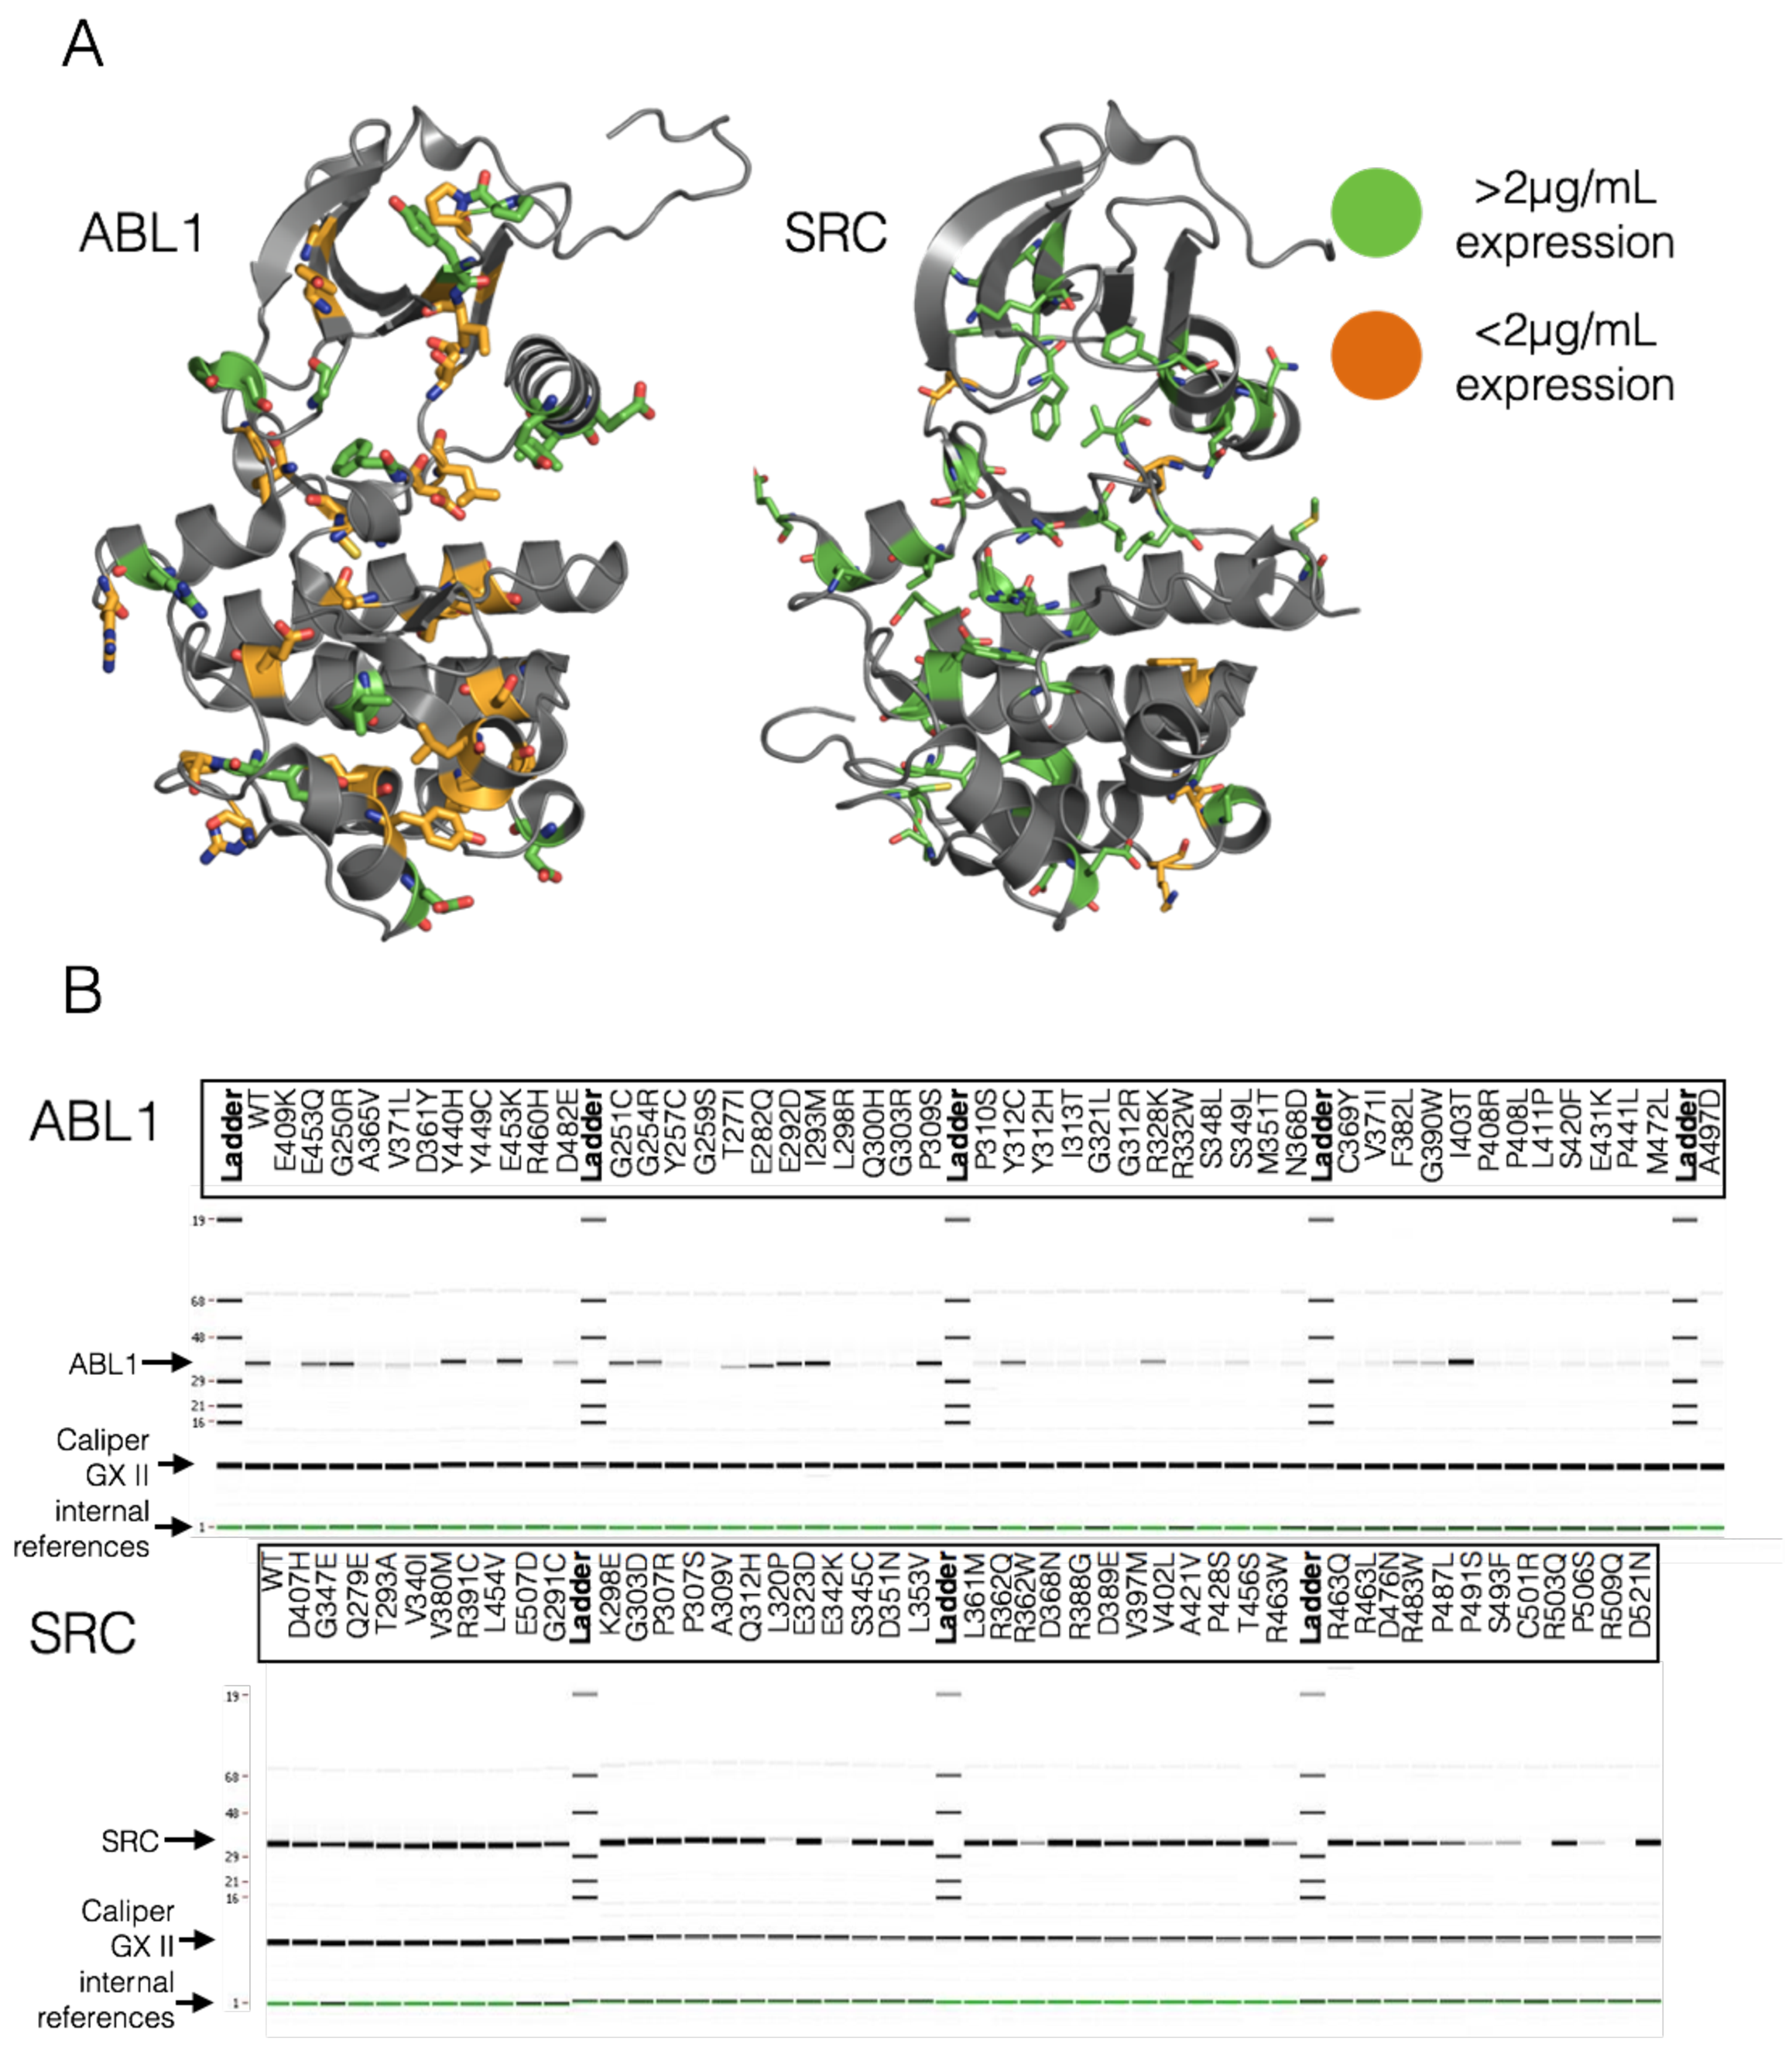
\includegraphics[width=0.5\linewidth]{figures/96-mutants-finalfigure.pdf}
		\caption[Expression yields for engineered clinically-derived Src and Abl missense mutants]{{\bf Expression yields for engineered clinically-derived Src and Abl missense mutants.}
			({\bf A}) All Abl and Src clinically-identified mutants assessed in the expression screen are displayed as sticks. 
			Mutants with expression yields $>$2~$\mu$g/mL are colored green, while those with yields $<$2~$\mu$g/mL are colored orange. 
			Rendered structures are Abl (PDBID: 2E2B) and Src (PDBID: 4MXO)~\citep{Levinson:2014gi}.
			({\bf B}) Synthetic gel images showing ABl (\emph{top}) or Src (\emph{bottom}) expression, with wells labeled by missense mutation.  
			Yield  was determined by Caliper GX II quantitation of the expected size band and reported in $\mu$g/mL culture, where total eluate volume was 120~$\mu$L following nickel bead pulldown purification from 900~$\mu$L bacterial culture.
			Residue mutations use numbering for the Uniprot canonical isoform.}
		\label{fig:96-mutant-fig}
	\end{figure}
\end{landscape}

\section{Methods}

\subsection{Semi-automated selection of kinase construct sequences for \emph{E.~coli} expression}

\subsubsection{Selection of human protein kinase domain targets}

Human protein kinases were selected by querying the UniProt API (query date 30 May 2014) for any human protein with a domain containing the string "protein kinase", and which was manually annotated and reviewed (i.e. a Swiss-Prot entry).
The query string used was:\\
{\tt taxonomy:"Homo sapiens (Human) [9606]" AND domain:"protein kinase" AND reviewed:yes}\\
Data was returned by the UniProt API in XML format and contained protein sequences and relevant PDB structures, along with many other types of genomic and functional information.
To select active protein kinase domains, the UniProt domain annotations were searched using the regular expression {\tt \^{}Protein kinase(?!; truncated)(?!; inactive)}, which excludes certain domains annotated "Protein kinase; truncated" and "Protein kinase; inactive".
Sequences for the selected domains, derived from the canonical isoform as determined by UniProt, were then stored.


\subsubsection{Matching target sequences with relevant PDB constructs}

Each target kinase gene was matched with the homologous in any other species, if present, and all UniProt data was downloaded.
This data included a list of PDB structures which contain the protein, and their sequence spans in the coordinates of the UniProt canonical isoform. PDB structures which did not include the protein kinase domain or truncated more than 30 residues at each end were filtered out. PDB coordinate files were then downloaded for each remaining PDB entry. The coordinate files contain various metadata, including the {\tt EXPRESSION\_SYSTEM} annotation, which was used to filter PDB entries for those which include the phrase "ESCHERICHIA COLI". The majority of PDB entries returned had an {\tt EXPRESSION\_SYSTEM} tag of "ESCHERICHIA COLI", while a small number had "ESCHERICHIA COLI BL21" or "ESCHERICHIA COLI BL21(DE3)".

The PDB coordinate files also contain SEQRES records, which should contain the protein sequence used in the crystallography or NMR experiment.
According to the PDB-101 (\url{http://pdb101.rcsb.org/learn/guide-to-understanding-pdb-data/primary-sequences-and-the-pdb-format}), the SEQRES should include the "sequence of each chain of linear, covalently-linked standard or modified amino acids or nucleotides. It may also include other residues that are linked to the standard backbone in the polymer." However, we found that these records are very often misannotated, instead representing only the crystallographically resolved residues.
Since expression levels can be greatly affected by insertions or deletions of only one or a few residues at either terminus~\citep{klock_combining_2008}, it is important to know the full experimental sequence. To measure the authenticity of a given SEQRES record, we developed a simple metric by hypothesizing that most crystal structures would likely have at least one or more unresolved residues at one or both termini and that the presence of an expression tag, which is typically not crystallographically resolved, would indicate an authentic SEQRES record.
To achieve this, unresolved residues were first defined by comparing the SEQRES sequence to the resolved sequence, using the SIFTS service to determine which residues were not present in the canonical isoform sequence~\citep{doi:10.1093/nar/gks1258}.
Regular expression pattern matching was used to detect common expression tags at the N- or C-termini.
Sequences with a detected expression tag were given a score of 2, while those with any unresolved sequence at the termini were given a score of 1, and the remainder were given a score of 0.
This data was stored to allow for subsequent selection of PDB constructs based on likely authenticity in later steps. The number of residues extraneous to the target kinase domain, and the number of residue conflicts with the UniProt canonical isoform within that domain span were also stored for each PDB sequence. 

\subsubsection{Plasmid libraries}

As a source of kinase DNA sequences for subcloning, we purchased three kinase plasmid libraries: the \href{https://www.addgene.org/human-kinase/}{Addgene Human Kinase ORF kit }, a kinase library from the Structural Genomics Consortium (SGC), Oxford (\url{http://www.thesgc.org}), and a kinase library from the \href{https://plasmid.med.harvard.edu/PLASMID/Home.xhtml}{PlasmID Repository} maintained by the Dana-Farber/Harvard Cancer Center. Annotated data for the kinases in each library was used to match them to the human protein kinases selected for this project.
The plasmid open reading frames (ORFs) were translated into protein sequences and aligned against the target kinase domain sequences from UniProt.
Also calculated were the number of extraneous protein residues in the ORF, relative to the target kinase domain sequence, and the number of residue conflicts with the UniProt sequence. Our aim was to subclone the chosen sequence constructs from these library plasmids into our expression plasmids. 

\subsubsection{Selection of sequence constructs for expression}

Of the kinase domain targets selected from UniProt, we filtered out those with no matching plasmids in our available plasmid libraries or no suitable PDB construct sequences.
For this purpose, a suitable PDB construct sequence was defined as any with an authenticity score greater than zero (see above). 
Library plasmid sequences and PDB constructs were aligned against each Uniprot target domain sequence, and various approaches were considered for selecting the construct boundaries to use for each target, and the library plasmid to subclone it from.
Candidate construct boundaries were drawn from two sources: PDB constructs and the SGC plasmid library, has been successfully tested for \emph{E.~coli} expression.

For most of the kinase domain targets, multiple candidate construct boundaries were available.
To select the most appropriate construct boundaries, we sorted them first by authenticity score, then by the number of conflicts relative to the UniProt domain sequence, then by the number of residues extraneous to the UniProt domain sequence span.
The top-ranked construct was then chosen.
In cases where multiple library plasmids were available, these were sorted first by the number of conflicts relative to the UniProt domain sequence, then by the number of residues extraneous to the UniProt domain sequence span, and the top-ranked plasmid was chosen.
This process resulted in a set of 96 kinase domain constructs, which (by serendipity) matched the 96-well plate format we planned to use for parallel expression testing.
We selected these constructs for expression testing.

An interactive table of the selected plasmids, constructs, and aligned PDB files can be viewed at \url{http://choderalab.org/kinome-expression}.

\subsubsection{Automation of the construct selection process}

While much of this process was performed programmatically, many steps required manual supervision and intervention to correct for exceptional cases.
While these exceptions were encoded programmatically as overrides to ensure the scheme could be reproduced from existing data, we hope to eventually develop a fully automated software package for the selection of expression construct sequences for a given protein family, but this was not possible within the scope of this work.

\subsection{Mutagenesis protocol}

Point mutations were introduced with a single-primer QuikChange reaction. 
Primers were designed to anneal at 55$^{\circ}$C both upstream and downstream of the point mutation, and with a total length of approximately 40 bases. 
At the codon to be modified, the fewest possible number of bases was changed. 
Plasmid template (160 ng) was mixed with 1 $\mu$M primer in 1x PfuUltra reaction buffer, with 0.8 mM dNTPs (0.2 mM each) and 1 U PfuUltra High-Fidelity DNA polymerase (Agilent), in a total volume of 20 $\mu$L. 
Thermocycler settings were 2 min at 95$^{\circ}$C, followed by 18 cycles of 20s at 95$^{\circ}$C, 1 min at 53$^{\circ}$C, 12 min at 68$^{\circ}$C (2min/kb), then 1 minute at 68$^{\circ}$C. 
After cooling to room temperature, 4 $\mu$L of the PCR reaction was added to 16 $\mu$L CutSmart Buffer (NEB) containing 10 U DpnI (NEB). 
After incubation for 2.5 hours at 37$^{\circ}$C, 6 $\mu$L of this mixture was used to directly transform XL1-Blue chemically competent cells (Agilent) according to the manufacturer’s protocol. 
Transformants were picked for plasmid mini-preps and the presence of the point mutations was confirmed by sequencing.

\subsection{Expression testing}

For each target, the selected construct sequence was subcloned from the selected DNA plasmid.
Expression testing was performed at the QB3 MacroLab (QB3 MacroLab, University of California, Berkeley, CA 94720) [\url{http://qb3.berkeley.edu/macrolab/}], a core facility offering automated gene cloning and recombinant protein expression and purification services.

Each kinase domain was tagged with a N-terminal His10-TEV and coexpressed with either the truncated YopH164 for Tyr kinases or lambda phosphatase for Ser/Thr kinases.
All construct sequences were cloned into the 2BT10 plasmid, an AMP resistant ColE1 plasmid with a T7 promoter, using ligation-independent cloning (LIC).
The inserts were generated by PCR using the LICv1 forward (TACTTCCAATCCAATGCA) and reverse (TTATCCACTTCCAATGTTATTA) tags on the primers.
Gel purified PCR products were LIC treated with dCTP. 
Plasmid was linearized, gel purified, and LIC-treated with dGTP.
LIC-treated plasmid and insert were mixed together and transformed into XL1-Blues for plasmid preps. 

Expression was performed in Rosetta2 cells (Novagen) grown with Magic Media (Invitrogen autoinducing medium), 100~$\mu$g/mL of carbenicillin and 100~$\mu$g/mL of spectinomycin. 
Single colonies of transformants were cultivated with 900~$\mu$L of MagicMedia into a gas permeable sealed 96-well block. 
The cultures were incubated at 37$^\circ$C for 4 hours and then at 16$^\circ$C for 40~hours while shaking. 
Next, cells were centrifuged and the pellets were frozen at -80$^\circ$C overnight. 
Cells were lysed on a rotating platform at room temperature for an hour using 700 $\mu$L of SoluLyse (Genlantis) supplemented with 400~mM NaCl, 20~mM imidazole, 1~$\mu$g/mL pepstatin, 1~$\mu$g/mL leupeptin and 0.5~mM PMSF. 

For protein purification, 500~$\mu$L of the soluble lysate was added to a 25~$\mu$L Protino Ni-NTA (Machery-Nagel) agarose resin in a 96-well filter plate. 
Nickel Buffer A (25~mM HEPES pH~7.5, 5\% glycerol, 400~mM NaCl, 20~mM imidazole, 1~mM BME) was added and the plate was shaken for 30~min at room temperature. 
The resin was washed with 2 mL of Nickel Buffer A. 
For the 96-kinase expression experiment, target proteins were eluted by a 2 hour incubation at room temperature with 10~$\mu$g of TEV protease in 80~$\mu$L of Nickel Buffer A per well and a subsequent wash with 40 $\mu$L of Nickel Buffer A to maximize protein release. 
Nickel Buffer B (25~mM HEPES pH~7.5, 5\% glycerol, 400~mM NaCl, 400~mM imidazole, 1~mM BME) was used to elute TEV resistant material remaining on the resin.
Untagged protein eluted with TEV protease was run on a LabChip GX II Microfluidic system to analyze the major protein species present. 

For the clinical mutant and Abl1 construct boundaries expression experiments, target proteins were washed three times with Nickel Buffer A prior to elution in 80 $\mu$L Nickel Buffer B. The eluted protein was run on a LabChip GX II Microfluidic system to analyze with major protein species were present. 


\subsection{Fluorescence-based thermostability assay}

To assess whether the highly-expressed wild-type kinase constructs are folded, a thermofluor thermostability assay~\citep{Lo:2004gy,Ericsson:2006dx,Matulis:2005dq} was performed for kinase constructs that have a minimum of 0.24~mg/mL protein concentration in the eluate. After diluting 9~$\mu$L of eluate by 1~$\mu$L dye, the effective assay concentration is 0.216~mg/mL minimum in 10~$u$L assay volume. Previous optimization efforts in the lab determined that 0.20~mg/mL was the lower limit of well-defined T$_m$ detection. This minimum concentration also ensured that the kinase was present at roughly an order of magnitude concentration higher than contaminating TEV protease. 

Kinase expression panel eluates, which were kept in 96-well deep well plate frozen at -80$^{\circ}$C for 2 years prior to the thermal stability assay, were thawed in an ice-water bath for 30 min. 9~$\mu$L of each kinase eluate was added to a 384 well PCR plate (4titude-0381). 
100X SYPRO Orange dye solution was prepared from a 5000X DMSO solution of SYPRO Orange Protein Gel Stain (Life Technologies, Ref S6650, LOT 1790705) by dilution in distilled water. In initial experiments, SYPRO Orange dye solution was diluted in kinase binding assay buffer (20~mM Tris 0.5~mM TCEP pH~8), which caused the dye to precipitate out of solution. 
Particulates in the dye solution were pelleted by tabletop centrifugation (2 min, 5000 RCF) and the solution was kept covered with aluminum foil in the dark to prevent photodamage. 
1~$\mu$L of 100X dye solution was added to each kinase eluate sample in 384-well PCR plate. 
The plate was sealed with Axygen UC-500 Ultra Clear Pressure Sensitive sealing film. 
To remove any air bubbles, the sample plate was centrifuged for 30~sec with 250~g using Bionex HiG4 centrifuge. 
Sample mixing was performed by orbital shaking with Inheco shakers for 2~min at~1000 RPM.

A thermofluor melt was performed using a LightCycler 480 (Roche) qPCR instrument using an excitation filter of 465~nm (half bandwidth 25~nm) and emission filter at 580~nm (half bandwidth 20~nm). 
LightCycler 480 Software Version 1.5.1 was used to operate the instrument and analyze the results. 
The temperature was held at 25$^{\circ}$C for 15 s before ramping up to 95$^{\circ}$C with a ramp rate of 0.06$^{\circ}$C/s.  
During temperature ramp 10 fluorescence acquisitions/$^{\circ}$C were recorded with dynamic integration time mode, melt factor of 1, quant factor of 10, and maximum integration time of 2~sec.  
Thermal protein denaturation causes hydrophobic patches of protein to be exposed, which SYPRO Orange dye can bind. 
Binding of SYPRO Orange dye is detected as an increase in fluorescence at 580~nm. 
Presence of a clear thermal denaturation peak in the absolute value of the derivative of the fluorescence as a function of temperature serves as an indication that the proteins were well-folded. 
Observed fluorescence was plotted as a function of temperature, and a melting temperature $T_m$ was determined as the maximum of the absolute value of its first derivative. 

\subsection{ATP-competitive inhibitor binding fluorescence assay}

To determine whether the expressed kinases had a well-folded ATP-binding site, we assessed whether the eluted kinase was capable of binding the ATP-competitive small molecule kinase inhibitor bosutinib.
We designed fluorescence-based binding assays following earlier work reporting that this quinoline-scaffold inhibitor undergoes a strong increase in fluorescence upon binding (even weakly) to kinase ATP-binding sites~\citep{levinson-boxer:plos-one:2012:bosutinib}.
By titrating in the ligand to close to the solubility limit, even weak binding to the ATP-binding site can be detected by observing emission increases around 450~nm during excitation at 280~nm.

For 33 of the kinases in our expression panel, 0.5~$\mu$M kinase solutions from kinase expression panel eluates were prepared in kinase binding assay buffer (20~mM Tris 0.5~mM TCEP pH~8) for a final volume of 100~$\mu$L in a black 96-well vision plate (4titude-0223). 
Six low-expressing kinases (Figure~\ref{fig:binding}, panels 39-44) were prepared by diluting 20~$\mu$L of eluate in kinase binding assay buffer (20~mM Tris 0.5~mM TCEP pH~8) to a final volume of 100~$\mu$L, for final concentrations below 0.5~$\mu$M. 
The plate was shaken for 2~min clockwise and 2~min counter-clockwise by orbital shaking with Inheco shakers at 2000~RPM and centrifuged for 30~sec with 1000~g using Bionex HiG4 centrifuge. 
Fluorescence emission spectra were measured from 370~nm to 600~nm (20~nm bandwidth) in 5~nm steps using 280~nm excitation (10~nm bandwidth) from both the top and bottom of the well using a Tecan Infinite M1000 PRO. 

Bosutinib free base (LC Labs, cat no.\ B-1788, lot no.\ BSB-103, M.W.\ 530.45 Da) was dispensed directly from a roughly 10~mM DMSO stock solution to the assay solution using a Tecan HP D300 Digital Dispenser. 
The 10~mM DMSO stock solution was prepared gravimetrically using an automated balance (Mettler Toledo Balance XPE205 with LabX Laboratory Software) by dispensing 39.02~mg solid Bosutinib powder stored under nitrogen gas at 25$^{\circ}$C into 8.0499~g DMSO (Alfa Aesar, cat no.\ 42780, log no.\ Y25B604, density 1.1004 g/mL at ambient temperature) which is kept dry under argon gas at 25$^{\circ}$C. 
To minimize atmospheric water absorption due to the hygroscopic nature of DMSO, the 10~mM stock solution was pipetted into wells of a 96-well stock plate by an automated liquid handling device (Tecan EVO 200 with air LiHa) and sealed with foil seal (PlateLoc).
Ligand was dispensed to the assay plate with HP D300 (using aliquots of stock solution pipetted from a freshly pierced stock plate well) targeting a roughly geometrically-increasing series of ligand concentrations in each well to achieve the following total ligand concentrations after each dispense: 0.008~$\mu$M, 0.013~$\mu$M, 0.023~$\mu$M, 0.038~$\mu$M, 0.064~$\mu$M, 0.109~$\mu$M, 0.183~$\mu$M, 0.308~$\mu$M, 0.519~$\mu$M, 0.875~$\mu$M, 1.474~$\mu$M, 3.174~$\mu$M, 6.037~$\mu$M, 10.862~$\mu$M, 18.991~$\mu$M. 
The plate was shaken by HP D300 for 10~sec after usage of each dispensehead.   
After each titration, the plate was shaken with Inheco shakers (2~min clockwise and counter-clockwise, 2000~RPM, orbital shaking) and centrifuged (30~sec, 1000~g) using a Bionex HiG4 centrifuge. Fluorescence spectra from 370~nm to 600~nm (bandwith 20~nm) in 5~nm steps using 280~nm excitation (bandwidth 10~nm) were read from both the top and bottom of the well using a Tecan Infinite M1000 PRO. 
In total, the experiment took 17.5~hours to complete due to the time-consuming spectral read after each dispense, likely resulting in significant evaporation from some wells during the experiment. 

ATP-competitive binding was analyzed qualitatively for each kinase by plotting the fluorescence spectra as a function of concentration to detect concentration-dependent increases in fluorescence. 
As a control for background ligand fluorescence independent of protein binding, fluorescence spectra of three replicates of ligand into buffer titrations were plotted. 
As a positive control, MK14 produced by a validated large scale expression protocol (see Supplementary Methods) from the same plasmid used in the high-throughput protocol was included. To control for non-specific binding to unfolded protein, we included boiled MK14 (prepared from the large scale expression of MK14 by boiling at 95$^{\circ}$C for 10~min). 
A concentration-dependent increase in fluorescence was interpreted as evidence that the ATP-binding site of the kinase was well folded and allowed for bosutinib binding. Due to the length of the experiment, it is possible that evaporation reduced the well volume below 100~$\mu$L and potentially caused bosutinib to reach higher concentration levels than expected. This creates uncertainty for data points, as bosutinib may either be a higher concentration (due to evaporation) or a lower concentration (due to potential precipitation caused by lower well volumes) than expected. 
For this reason, we have interpreted the experiment as qualitative evidence of binding, instead of quantitatively. 
Bosutinib binding is an indication of proper folding of the ATP binding pocket of these recombinantly expressed kinase constructs. 

\subsection{Large Scale expression and purification protocol for MK14}


Large scale expression of MK14 was performed  at the QB3 MacroLab (QB3 MacroLab, University of California, Berkeley, CA 94720 [\url{http://qb3.berkeley.edu/macrolab/}], a core facility offering automated gene cloning and recombinant protein expression and purification services.

Rosetta2(DE3)pLysS cells (Novagen) were used to co-express MK14 (same plasmid as from the high-throughput kinase expression panel) and 13SA Lamda phosphatase. The cells were grown in 2YT Medium (16~g/L Tryptone, 10~g/L Yeast Extract, 5~g/L NaCl) to OD600 of 0.5 at 37$^{\circ}$C. The culture was cooled to 16$^{\circ}$C and induced with 0.5~mM IPTG overnight. The cultures were pelleted at 5000~rpm for 30~min and resuspended in 20~mL Nickel buffer A (25~mM HEPES pH~7.5, 10\% glycerol, 400mM NaCl, 20~mM imidazole, 5~mM BME) with the following protease inhibitors: 1~$\mu$g/mL leupeptin, 1~$\mu$g/mL pepstatin, and 0.5~mM PMSF). The resuspended cells were frozen at -80$^{\circ}$C. 

When ready for purification, the cells were thawed and ruptured using a homogenizer (Avestin C3, 15000psi, 3 passes). The broken cells were pelleted at 15000~rpm for 30~min (SS34 rotor). Clarified lysate was loaded onto a  5~mL HisTrap FF Crude column (GE Healthcare) and washed with Nickel buffer A to remove any unbound material. The protein was eluted with Nickel buffer B (25~mM HEPES pH~7.5, 10\% glycerol, 400mM NaCl, 400~mM imidazole, 5~mM BME) and pooled for buffer exchange into Nickel buffer A on a HiPrep 26/10 Desalting Column (GE Healthcare). Rough protein yields were quantified using theorectical extinction coefficients calculated using ProtParam (http://ca.expasy.org/tools/protparam.html). The His tag was cleaved off of MK14 by incubation with TEV protease (25$^{\circ}$C, 2 hours, 1:20 mass ratio). 

After tag cleavage, the sample was run over a 5~mL HisTrap FF Crude column (GE Healthcare) with Nickel buffer A. 
The flow-through was collected, concentrated to roughly 5mL using centrifugal concentrators (10~kDA MWCO, Millipore) and loaded onto a HiPrep 16/60 Sephacryl S-200 HR column (GE Healthcare). 
The sample was equilibrated into Gel Filtration buffer (20 mM Tris-HCl pH 8.0, 150 mM NaCl, 5\% glycerol, 1 mM DTT) and fractions containing MK14 were pooled and concentrated (10~kDA MWCO centrifugal concentrators, Millipore). 
500~$\mu$L aliquots of MK14 were snap frozen in liquid nitrogen and stored at -80$^{\circ}$C. Quantification by theoretical extinction coeffcient suggests the final MK14 concentration was roughly 4.0~mg/mL (97~$\mu$M), roughly 22.4~mg/L of culture yield.  

\section{Discussion}
\label{section:discussion}

We have demonstrated that a simple, uniform, automatable protocol is able to achieve useful bacterial expression yields for a variety of kinase domain constructs.
While yields could likely be further improved by a variety of methods---such as the addition of solubility-promoting tags, construct domain boundary and codon optimization, or mutations to improve the solubility or ablate catalytic activity---the simplicity of this approach suggests widespread utility of automated bacterial expression for biophysical, biochemical, and structural biology work for the further study of human kinase domains.

Our expression test of 81 different construct boundaries of the Abl kinase domain demonstrated a surprising sensitivity of expression yields to the precise choice of boundary. 
This sensitivity may be related to where the construct is truncated with respect to the secondary structure of the protein, as disrupting secondary structure could cause the protein to improperly fold, leading to low soluble protein yield even when total expression is high. 
Of note, the highest expressing C-terminal boundaries for Abl were residues 511 and 512. 
These residues fall in the regulatory alpha helix~$\alpha$I~\citep{Nagar:2003tu}. 
This helix has been shown to undergo a dramatic conformational change upon binding to the myristoylated N-terminal cap, which introduces a sharp "kink" in residues 516--519. 
These residues may lead to higher levels of soluble expression by truncating an secondary structural element that is unusually flexible. 
Indeed, this helix is not resolved in some X-ray structures (PDBID:2E2B)~\citep{Horio:2007wo}, further suggesting that this helix is less thermodynamically stable than expected. 
Control replicates of three constructs indicate good repeatability of expression yields in the high-throughput format. 
This screen suggests that optimization of construct boundaries could potentially further greatly increase yields of poorly expressing kinase domains. 
Codon optimization for bacterial expression could also increase expression for kinase domains with low yield due to codon bias~\citep{SORENSEN2005113}, as could coexpression with chaperones~\citep{Haacke:ProteinExpr.Purif.:2009}. 

For those kinases that did express, a fluorescence-based thermostability assay indicated that many of the highest-expressing kinases are well folded. 
An ATP-competitive inhibitor binding fluorescent assay provides qualitative evidence that the 39 kinases that had sufficiently high expression levels to be assayed have a well-formed ATP-binding site capable of binding bosutinib, a small molecule ATP-competitive kinase inhibitor. 
Taken together, these two experiments demonstrate that our expression protocol produces folded kinases with utility for biophysical experiments and drug design.  

The tolerance of these bacterial constructs to many engineered clinical missense mutations suggests a promising route to the high-throughput biophysical characterization of the effect of clinical mutants on anticancer therapeutics. 
Mutations that did not express well may destabilize the protein, or may increase the specific activity of the kinase. 
A higher specific activity would require more phosphatase activity, wasting ATP to prevent high levels of phosphorylation that have been hypothesized to cause difficulty expressing kinases without a coexpressed phosphatase in bacteria~\citep{seeliger:2005:protein-sci:kinase-expression}. 
Mutations that are destabilizing may show improved expression if coexpressed with more elaborate chaperones such as GroEL and Trigger factor~\citep{Haacke:ProteinExpr.Purif.:2009}.
Mutations that increase the specific activity of the kinase might also express better when combined with an inactivating mutation.  

High-throughput automated kinase expression could be combined with enzymatic or biophysical techniques for characterizing the potency of a variety of clinical kinase inhibitors to assess which mutations confer resistance or sensitivity.
While the process of engineering, expressing, purifying, and assaying mutants currently takes approximately two weeks, it is possible that new techniques for cell-free bacterial expression~\citep{Kim:Biotechnol.Bioeng.:1999,Sawasaki:Proc.Natl.Acad.Sci.:2002a} may reduce this time to a matter of days or hours in a manner that might be compatible with clinical time frames to impact therapeutic decision-making.

We hope that other laboratories find these resources useful in their own work.


%%%%%%%%%%%%%%%%%%%%%%%%%%%%%%%%%%%%%%%%%%%%%%%%%%%%%%%%%%%%%%%%%%%%%%%%%%%%%%%%%%%%%%%%%%%%%%%%%%%%%%
% Acknowledgments 
%%%%%%%%%%%%%%%%%%%%%%%%%%%%%%%%%%%%%%%%%%%%%%%%%%%%%%%%%%%%%%%%%%%%%%%%%%%%%%%%%%%%%%%%%%%%%%%%%%%%%%
\section{Author Contributions}

Conceptualization, JDC, DLP, SKA, MI, LRL, SMH, NML, MAS; Methodology, DLP, MI, LRL, SMH, SKA, JDC, NML, MAS; Software, DLP, JDC, SMH; Formal Analysis, SKA, JDC, MI, SMH; Investigation, MI, LRL, SG, CJ, SKA, SMH; Resources, CJ, SG;  Data Curation, SKA, MI, LRL, DLP, JMB; Writing-Original Draft, SKA, LRL, DLP, JDC, SG, SMH, MI; Writing - Review and Editing, SKA, JDC, MI, LRL, SHM, SG, CJ, NML, MAS; Visualization, SKA, JDC, MI, SMH; Supervision, JDC, NML, MAS; Project Administration, SKA, JDC, MI, SMH; Funding Acquisition, JDC, SMH


%%%%%%%%%%%%%%%%%%%%%%%%%%%%%%%%%%%%%%%%%%%%%%%%%%%%%%%%%%%%%%%%%%%%%%%%%%%%%%%%%%%%%%%%%%%%%%%%%%%%%%
% Acknowledgments 
%%%%%%%%%%%%%%%%%%%%%%%%%%%%%%%%%%%%%%%%%%%%%%%%%%%%%%%%%%%%%%%%%%%%%%%%%%%%%%%%%%%%%%%%%%%%%%%%%%%%%%
\section{Acknowledgments}

DLP, SMH, LRL, SKA, MI, and JDC acknowledge support from the Sloan Kettering Institute.
This work was funded in part by the Marie-Josée and Henry R. Kravis Center for Molecular Oncology, the National Institutes of Health (NIH grant R01 GM121505 and National Cancer Institute Cancer Center Core grant P30 CA008748), the Functional Genomics Institute (FGI) at MSKCC, and a Louis V.~Gerstner Young Investigator Award. 
MAS acknowledges funding support by NIH grant R35 GM119437. 
The authors are grateful to Gregory Ross (MSKCC) for assistance in preparing the computational infrastructure for selecting clinical point mutants, and to Sarah E.~Boyce (current address: Schr\"{o}dinger, New York, NY) for assistance with multiple stages of this project.
We gratefully acknowledge the members of the MSKCC Molecular Diagnostics Service in the Department of Pathology for their efforts in collecting and compiling mutations for Abl and Src kinases used here.
We thank the Kuriyan lab for the gift of pCDFDuet1-YOPH plasmid.
The authors are grateful to \href{http://www.addgene.org}{Addgene} for their help in making the plasmids generated by this work available to the research community at minimal cost.

\realsinglespacing
\bibliographystyle{vancouver-elife.bst}
\bibliography{albanese}
\end{document}
